\documentclass[a4paper, 12pt]{book}
\usepackage[toc,page]{appendix}
\usepackage{booktabs}
\usepackage{natbib}
\usepackage{textcomp}
\usepackage[automake,nonumberlist]{glossaries} %automake can automatic compile to generate .glo
\usepackage{graphicx}
\usepackage{enumitem}
\usepackage{booktabs}
\usepackage{pdflscape}
\usepackage{array}
\usepackage[justification=raggedright, singlelinecheck=on, font={normalsize, rm}, labelfont=bf]{caption} %singlelinecheck=centre short caption
\usepackage{threeparttable} % Add table annotation
\usepackage{rotating} % Rotate the tables
\usepackage{subcaption}
\usepackage{times}    % Times ne6w romans
\usepackage{placeins}
\usepackage{pdfpages}
\usepackage{amssymb,amsmath}
\usepackage{tikz}
\newcommand*{\pd}[3][]{\ensuremath{\frac{\partial^{#1} #2}{\partial #3}}} % in order to write partial derivative
\usetikzlibrary{calc,shapes.geometric,arrows,positioning}
\usetikzlibrary{matrix,positioning,decorations.pathreplacing}
\usepackage{geometry}
\usetikzlibrary{decorations.pathreplacing}
\usepackage{xcolor}
\usepackage[makeroom]{cancel}
\usepackage{siunitx} 
\usepackage{gensymb} % only need this when compiled at home
\sisetup{detect-all}
\usepackage{makecell}
\usepackage{array}
\usepackage{bm,upgreek}
\usepackage{colortbl}
\usepackage[percent]{overpic}
\usepackage{minibox}
\usepackage[thinlines]{easytable}
\usepackage{multirow}
\usepackage{tabularx}
\usepackage[nottoc,notlof,notlot]{tocbibind} 
\usepackage{pict2e}
\usepackage{float}


\usepackage{fancyhdr} % To customize the footer and header in your document
\setlength{\headheight}{15.2pt} % Change the latter size
\addtolength{\oddsidemargin}{1.5cm} % Add left side of odd page margin with 1.5cm
\addtolength {\evensidemargin}{-1.5cm} % Reduce left side of even page margin with 1.5cm
\pagestyle{fancy} % The "fancy" style is set by \pagestyle{fancy}

% If your document is double-sided, for example a book, and you need to customize the header and the footer, the recommended commands in this case are \fancyhead and \fancyfoot
\fancyhead{}
\fancyfoot{}
\fancyhead[LO, RE]{\thepage} % Show page number on left side of odd page and right side of even page
\fancyhead[RO, LE]{\small\rightmark} % Show Section name on right side of odd page and left side of even page. In the 'book' class, /leftmark represents the chapter name, /rightmark represents the section name. Here we show the section name on the header.

\usepackage{setspace}
%\onehalfspacing 
\doublespacing

\graphicspath{{./images/}{./chptMethod/images/}}
\DeclareGraphicsExtensions{.pdf,.png,.jpg,.eps}  

\makeindex
\makeglossaries
%  'makeglossaries thesis' command line

%\newacronym{}{}{}

\newacronym{ipf}{IPF}{idiopathic pulmonary fibrosis}
\newacronym{2d}{2D}{two dimension}
\newacronym{3d}{3D}{three dimension}
\newacronym{ct}{CT}{Computed tomography}
\newacronym{hrct}{HRCT}{high resolution computed tomography}
\newacronym{abm}{ABM}{adaptive border marching}
\newacronym{mad}{MAD}{mean absolute distance}
\newacronym{rasm}{RASM}{robust active shape model}
\newacronym{roi}{ROI}{region of interest}
\newacronym{map}{MAP}{maximum a posteriori}
\newacronym{tps}{TPS}{thin plate spline}
\newacronym{ssm}{SSM}{statistical shape model}
\newacronym{asm}{ASM}{active shape model}
\newacronym{sfeal}{SFeaL}{Statistical Finite element analysis of Lobe}
\newacronym{aging}{AGING}{human aging cohort}
\newacronym{hla}{HLA}{Human Lung Atlas}
\newacronym{hdec}{HDEC}{Health and Disability Ethics Committees}
\newacronym{iclic}{I-Clic}{Iowa Comprehensive Lung Imaging Center}
\newacronym{dof}{DoF}{degrees of freedom}
\newacronym{pca}{PCA}{principal component analysis}
\newacronym{rms}{RMS}{root mean square}
\newacronym{gpa}{GPA}{General Procrustes Alignment}
\newacronym{ild}{ILD}{interstitial lung disease}
\newacronym{qol}{QOL}{quality of life}
\newacronym{uip}{UIP}{usual interstitial pneumonia}
\newacronym{iip}{IIP}{idiopathic interstitial pneumonia}
\newacronym{ger}{GER}{gastroesophageal reflux}
\newacronym{ats}{ATS}{American Thoracic Society}
\newacronym{ers}{ERS}{European Respiratory Society}
\newacronym{mdd}{MDD}{multidisciplinary discussion}
\newacronym{tlc}{TLC}{total lung capacity}
\newacronym{dlco}{DLCO}{diffusion capacity of the lung for carbon monoxide}
\newacronym{cpfe}{CPFE}{''combined pulmonary fibrosis and emphysema''}
\newacronym{ph}{PH}{pulmonary hypertension}
\newacronym{fev1}{$\mathrm{FEV_1}$}{forced expiratory volume in 1 second}
\newacronym{fvc}{FVC}{forced vital capacity}
\newacronym{fev1/fvc}{$\mathrm{FEV_1/FVC}$}{ratio of the forced expiratory volume in the one second to the forced vital capacity of the lungs}
\newacronym{kco}{KCO}{carbon monoxide transfer coefficient}
\newacronym{mld}{MLD}{mean lung density}
\newacronym{hist}{HIST}{histogram analysis}
\newacronym{cad}{CAD}{computer-aided diagnosis}
\newacronym{ltrc}{LTRC}{Lung Tissue Research Consortium}
\newacronym{vois}{VOIs}{volumes of interest}
\newacronym{mds}{MDS}{multi-dimensional scaling}
\newacronym{cvm}{CVM}{Cramer Von Mises Distance}
\newacronym{pfts}{PFTs}{pulmonary function tests}
\newacronym{rv}{RV}{residual volume}
\newacronym{frc}{FRC}{functional residual capacity}
\newacronym{vc}{VC}{vital capacity}
\newacronym{tv}{TV}{tidal volume}
\newacronym{ic}{IC}{inspiratory capacity}
\newacronym{irv}{IRV}{inspiratory reserve volume}
\newacronym{erv}{ERV}{expiratory reserve volume}
\newacronym{aic}{AIC}{Akaike information criterion}
\newacronym{bic}{BIC}{Bayesian information criterion}
\newacronym{rdh}{$\mathrm{R_dH}$}{Horsfield diameter ratios}
\newacronym{rds}{$\mathrm{R_dS}$}{Strahler diameter ratio}
\newacronym{rbc}{RBC}{red blood cell}
\newacronym{paao2}{$\mathrm{P_{A-a} O_2}$}{alveolar-arterial pressure difference for oxygen}
\newacronym{dpld}{DPLD}{diffuse parenchymal lung diseases}
\newacronym{pvv}{PVV}{pulmonary vessel volume}
\newacronym{adhb}{ADHB}{Auckland District Health Board}
\newacronym{nsip}{NSIP}{non-specific interstitial pneumonia}
\newacronym{copd}{COPD}{chronic obstructive pulmonary disease}
\newacronym{amfm}{AMFM}{adaptive multiple feature method}
\newacronym{anns}{ANNs}{artificial neural networks}
\newacronym{qlf}{QLF}{quantitative lung fibrosis}
\newacronym{laa}{LAA}{low attenuation areas}



\usepackage[hidelinks,pagebackref]{hyperref}
\renewcommand*{\backref}[1]{}
\renewcommand*{\backrefalt}[4]{[{\small%
    \ifcase #1 Not cited.%
          \or Cited on page~#2.%
          \else Cited on pages #2.%
    \fi%
    }]}

\usepackage{hypcap}

\begin{document}
\frontmatter

\begin{titlepage}
  \begin{center}
    \vfill
    {\Large \textbf{Idiopathic pulmonary fibrosis: a study using volumetric imaging and functional data in a computational lung model}} % \textbf is for bold font
    \\[6cm]
    Yuwen Zhang
    \vfill
    \normalsize A thesis submitted in fulfilment of the requirements for the degree of Doctor of Philosophy in Bioengineering. \\[1cm]
    This thesis is for examination purposes only and is confidential to the examination process.
    \vfill
    Auckland Bioengineering Institute
    \\[0.8cm] The University of Auckland
    \\[0.8cm] 2018
  \end{center}
\end{titlepage}

\cleardoublepage
\chapter*{Abstract}
Idiopathic pulmonary fibrosis (IPF), the most aggressive and frequent form of idiopathic interstitial pneumonias (IIPs), is a chronic and life-threatening disease of unknown cause. It is characterised by progressive worsening of dyspnea and lung function and is associated with a poor prognosis. IPF occurs primarily in middle-aged and elderly adults, and is more frequent in males than females. Even worse, the aetiology of IPF remains elusive, and its progression is variable and unpredictable, hence there are no biomarkers that can indicate the likely progression of the disease. A quantification scheme that allows recognition of disease consistently across radiology, pulmonary and pathology disciplines remains difficult. In this study, a combination of quantitative information extracted from HRCT, clinical knowledge, and computational modelling was developed to help with a better understanding of the progression of IPF and investigate strategies for patient-specific diagnosis and treatment planning for IPF patients.

First, an automatic lung lobe segmentation method from HRCT images was developed, which is guided by a statistical shape model that can predict the likely region of fissure locations. This new method was able to estimate the fissure location in 100\% of cases including both normal healthy and IPF subjects, whereas two comparison segmentation softwares that use anatomy-based methods fail in several cases with lobes segmented. Second, tissue abnormalities in IPF lungs were classified, and then mapped to a statistical shape model, and quantitative approaches were used to analyse lung shape, tissue density, tissue volume, the spatial distribution of abnormalities, and regional changes in tissue over time. Fibrosis was found to present predominantly basally and peripherally in the lung. In contrast, emphysema in these subjects mostly located in upper lobes. The first principal statistical shape mode ($>20\%$ of the shape variation in normal lungs) is significantly different between IPF and normal and strongly correlated with fibrosis extent in IPF lungs. Finally, a computational model of lung function was developed which integrated quantification analysis from volumetric CT data and pulmonary functional test to understand differences between IPF and normal older lungs. Ventilation, perfusion and gas exchange models were parameterized to simulate $\dot{V}$, $\dot{Q}$ distribution and gas transport. The computational model can reasonably predict the patient-specific ventilation, perfusion and gas exchange in IPF lung, and quantify the difference of lung function between IPF patients and older normal people. However, abnormalities on volumetric CT imaging may be not able to provide enough information to explain the decline of lung function in IPF patient, and an individual impaired gas exchange appears to happen in not only abnormally tagged region but also in CT-visualized 'normal' tissues.

IPF is a complex and progressive disease that has multifarious physiological processes and significant individual differences. The methods and models presented in this thesis provide a basis for application to research in IPF lung function, and furthers investigations into the underlying relationship between physiology mechanisms and disease progressions of IPF.

\addcontentsline{toc}{chapter}{Abstract}

\cleardoublepage
\chapter*{Acknowledgements}
I would like to use this opportunity to express my gratitude to everyone who contributed to this research and supported me throughout my PhD. 

First and foremost, I would like to express my sincere gratitude to my supervisor Professor Merryn Tawhai, Dr Alys Clark and  Dr Haribalan Kumar for the tremendous patience, motivation, enthusiasm, and immense knowledge. Their continuous guidance helped me in all the time of research and writing of this thesis. This thesis would not be completed without their valuable advice and unfailing trust. It is my great honour to be their student and to have worked under their supervision.

I would like to thank Brian Bartholmai from Mayo Clinic for providing CALIPER classification data, and thank Dr David Milne and Dr Margaret Wilsher from Auckland Hospital for providing the CT image data of IPF patients. Without their constant assistance, this research would not have been possible.

I am also great thankful for the amazing people of lung and placenta groups: Mahyar, Hamed, Zay, Amir, Luca, Behdad, Toby, Kelly, Kerry, Rojan, Win, Mabelle and Izza. My special thanks goes to my lovely friends: Nancy, Wendy and Si. Thank you for giving me so much help, warm and happiness during my PhD.

A big thank to my family for supporting me spiritually throughout my life. Last but not the least, my deepest gratitude to my beloved husband, Xinjian. Thanks for accompanying me, encouraging me, supporting me and loving me. Words would never say how grateful I am to you. Thank you! 

\addcontentsline{toc}{chapter}{Acknowledgement}

% table of contents
\cleardoublepage
\renewcommand{\contentsname}{Table of Contents}
\tableofcontents
\addcontentsline{toc}{chapter}{\contentsname}

%  list of figures
\cleardoublepage
\listoffigures
\addcontentsline{toc}{chapter}{\listfigurename}

%  list of tables
\cleardoublepage
\listoftables
\addcontentsline{toc}{chapter}{\listtablename}

%  glossaries
\printglossary[type=\acronymtype,title={List of Abbreviations}]
%\printglossaries
\addcontentsline{toc}{chapter}{List of Abbreviations}

\mainmatter  
%\chapter{Introduction} \label{Yuwen_Introduction}
\section{Motivation}
Idiopathic pulmonary fibrosis (IPF) is a lethal fibrosing lung disorder that typically affects adults in the sixth to seventh decade of life \citep{meltzer2008idiopathic,king2011idiopathic}. IPF is more frequent in males than females, and is associated with environmental factors such as smoking or dust exposure, but as its name suggests does not have a clear aetiology. There is no known cure, although some very new therapies have been suggested to slow the rate of physiologic decline \citep{raghu2011official}. IPF belongs to the family of \gls{ild}, and is the most frequently diffuse occurring interstitial lung disease \citep{meltzer2008idiopathic}. In IPF lungs, healthy tissues are gradually replaced by an abnormal and excessive deposition of collagen (fibrosis), which may lead to a reduction in lung volumes, decreased lung compliance, mismatching at ventilation and perfusion, impaired gas exchange, and ultimately respiratory failure and death \citep{richeldi2017idiopathic}.

Diagnosis of IPF relates to a histopathological or radiological pattern typical of \gls{uip} \citep{raghu2011official,xaubet2017idiopathic}. UIP pattern is usually associated with honeycombing (subpleural cystic airspaces with well-defined walls),  reticular opacities and ground-glass abnormalities \citep{raghu2011official,richeldi2017idiopathic}. These abnormalities in IPF typically develop preferentially in posterior-basal lung regions, and often co-exists with emphysema, which causes a progressive and irreversible decline in lung function. Currently it is not clear how - or whether - the spatial distribution of tissue abnormalities in IPF (including classifications of tissue type) correlate with \gls{pfts}. In addition, the progression of IPF is variable between individuals, and no established quantitative tools exist to assess its development and how the tissue abnormalities change over time in this condition. Therefore, developing a computational modelling of lung function in IPF over time, together with clinical knowledge, will be helpful for clinician to have a better understanding of patient prognosis, and presents potential novel ways of investigating strategies for patient-specific diagnosis and treatment planning for IPF patients.

\section{Thesis objectives} \label{ThesisObjective}
The primary aim of this thesis is to contribute toward developing a new quantitative tool that integrates data from volumetric imaging, PFTs, and computational models for lung function, to take steps toward predicting the development of IPF over time, and to understand differences, including lung shape and lung function, between IPF and normal older lungs. 

The specific objectives of this thesis are:

\paragraph{Objective 1:} Develop an automatic lung lobe segmentation method based on HRCT images that can consistently estimate lobar boundaries even if the boundary is not clear along its entire length. The method needs to be tested on both healthy subjects and IPF subjects. Ideally the algorithm will be automatic, or semi-automatic.
\paragraph{Objective 2:} Classify and quantify tissue abnormalities from HRCT scans of IPF lungs. Analyse the density, volume, spatial distribution, and their change over time.
\paragraph{Objective 3:} Investigate the difference of lung shape between IPF and older normal lungs, and explore the correlation of lung shape change in IPF with the extent fibrosis.
\paragraph{Objective 4:} Integrate the image-based tissue quantification, pulmonary functional test and computational modeling to simulate the lung function in IPF, compared with the older normal people, and to use these tools to estimate the impact of CT features of IPF on lung function.

\section{Thesis overview}
\paragraph{Chapter 2} In order to quantitatively explore the link between structure and lung function of patients with IPF, some background knowledge of this disease is summarized in this chapter. The first part provides an basic introduction of IPF, including its epidemiology, adetiology, pathogenesis, diagnosis, clinical courses and comorbidities. The second part describes some physiological alterations in IPF lungs. The changes in the mechanical properties of the lungs in IPF and the changes in pulmonary gas exchange are discussed in details.
\paragraph{Chapter 3} Automatic identification of pulmonary lobes from imaging is important for the further image-based analysis of lung function and disease progression. In order to overcome difficulties in identifying pulmonary fissures, especially in disease, a statistical finite element shape model of lobes is applied to guide lobar segmentation in this chapter. By deforming a principal component analysis based statistical shape model onto an individual’s lung shape, the likely region of fissure locations is predicted to initialize the search region for fissures. Then, an eigenvalue of Hessian matrix analysis and a connected component eigenvector based analysis are used to determine a set of fissure-like candidate points. A smooth multi-level B-spline curve is fitted to the most fissure-like points (those with high fissure probability) and the fitted fissure plane is extrapolated to the lung boundaries. The method is tested on 20 inspiratory and expiratory CT scans, and compared with existing algorithms in healthy young subjects and older subjects with IPF.

\begin{itemize}
  \item Yuwen, Z., Mahyar O., Alys, R., Hari, K., Margaret, L.W., David, G.M., Eric, A.H., and Merryn, H.T. (2019, February). Pulmonary lobar segmentation from computed tomography scans based on a statistical finite element analysis of lobe shape. In: SPIE Medical Imaging, International conference. San Diego, USA.
\end{itemize}

\paragraph{Chapter 4} This chapter outlines the study of quantitative analysis of IPF disease features in HRCT scans, including both tissue abnormality quantification and lung lobe shape analysis, to provide consistent potential tissue-level and shape-level biomarkers that can indicate the likely progression of the disease over time. Lung tissues are classified as normal, reticular, ground glass, or emphysema using CALIPER (Computer-Aided Lung Informatics for Pathology Evaluation and Ratings) software. The classified data is then mapped to a \gls{ssm}, which allows a reliable comparison between different patients or within one patient of different time points. Quantitative approaches are used to analyse tissue density, tissue volume, the spatial distribution of abnormalities, and regional changes in tissue over time. Principal component analysis (PCA) based SSM is applied to understand lung shape differences between IPF and normal older lungs through quantifying principal modes of shape variation of both IPF and old normal subjects. 

\begin{itemize}
  \item Yuwen, Z., Alys, R., Hari, K., Brian, B.J, and Merryn, H.T. (2017, November). Quantitative analysis of idiopathic pulmonary fibrosis abnormality from CT imaging. In: 13th Engineering Mathematics and Applications Conference, International conference. Auckland, New Zealand.
	\item Yuwen, Z., Alys, R., Hari, K., David, G.M., Margaret, L.W., Brian, B.J, and Merryn, H.T. (2018, March). High resolution CT-based characterization analysis of idiopathic pulmonary fibrosis. In: the Thoracic Society of Australia \& New Zealand (TSANZ) conference, International conference. Adelaide, Australia.
\end{itemize}

\paragraph{Chapter 5} In this chapter, data from volumetric imaging, quantitative tissue-level and shape-level features, and PFT are integrated to guide a patient-specific computational models of lung function of IPF. In order to make a comparison of lung function between IPF patients and older normal people, for each patient, a subject-specific lung mesh that represents the lung shape of old normal individual with the same age, BMI and pulmonary functional data is predicted using SSM. Anatomically based airway and blood vessel trees are generated derived from HRCT images, and are matched to the IPF lung mesh and the corresponding old normal lung mesh. The ventilation, perfusion and gas exchange models are then used to simulate $\dot{V}$, $\dot{Q}$ distribution and gas transport in normal and IPF lungs.

\begin{itemize}
  \item Yuwen, Z., Mahyar O., Alys, R., Hari, K., David, G.M., Margaret, L.W., Eric, A.H., and Merryn, H.T. (2018, March). Idiopathic pulmonary fibrosis: a study using volumetric imaging and functional data in a computational lung model, International conference. San Diego, USA.
\end{itemize}

\paragraph{Chapter 6} Key findings of this thesis are summarized in this chapter, with discussion of the main methods, models and outcomes. Potential future directions that need to be addressed to develop the modelling framework are also discussed. 

%\chapter{Background} \label{Yuwen_Background}
To quantitatively explore the link between lung structure and function of patients with idiopathic pulmonary fibrosis (IPF), some background knowledge of the disease is required. This chapter provides an introduction to IPF epidemiology, aetiology, pathogenesis, diagnosis, clinical course, comorbidities, and physiological alterations.

%%%%%%%%%%%%%%%%%%%%%%%%%%%%%%%%%%%%%%%%%%%%%%%%%%%%%%%%%%%%%%%%%%%%%%%%%%%%5
\section{Introduction to idiopathic pulmonary fibrosis} 
\subsection{Definition} 
Idiopathic pulmonary fibrosis is a chronic, progressive, irreversible, and lethal lung disease of unknown cause. It usually manifests over several years during which progressive scarring occurs in the supporting structural framework (interstitium) of the lung tissue \citep{meltzer2008idiopathic, raghu2011official}. It is the scarring of the tissue that is termed fibrosis. This fibrotic condition is generally thought to result from abnormal wound healing after repeated pulmonary tissue damage \citep{king2011idiopathic}. Several causes of alveolar injury have been implicated in IPF, including cigarette smoke, environmental exposure to toxins (e.g. asbestos, avian toxins), gastro-oesophageal reflux, viral infection, and internal mechanisms such as autoimmunity, genomic instability or telomerase length \citep{raghu2011official, ahluwalia2014new}.

In IPF patients' lungs, some healthy tissues are replaced by altered extracellular matrix and a destroyed alveolar architecture, which leads to decreased lung compliance, disrupted gas exchange, and ultimately respiratory failure and death \citep{richeldi2017idiopathic}. The fibrosing areas are generally observed to arise first at the basal and peripheral region of the lungs, and then gradually progress to involve all lung tissues \citep{martinez2017idiopathic}. The prominent symptoms of IPF are exercise-induced breathlessness and chronic dry cough \citep{meltzer2008idiopathic}, which will eventually have a devastating effect on a patient’s \gls{qol} \citep{kim2015natural}. IPF usually affects middle-aged and elderly adults (median age at diagnosis 66 years, range 55-75 years). The disease is isolated to the lungs, and is associated with the radiological and/or histological pattern of UIP \citep{king2011idiopathic,raghu2011official,xaubet2017idiopathic}. A typical UIP pattern is usually characterised by ‘honeycombing’, traction bronchiectasis, and peripheral alveolar septal thickening \citep{martinez2017idiopathic}, which will be introduced briefly in Section \ref{RadiographicFeatures}.

\subsection{Disease classification} 
IPF belongs to the family of interstitial lung disease (ILD) or, more accurately, the \gls{dpld}. All ILDs result in damage to the lung interstitium, with varying patterns of inflammation and fibrosis. Within the broad category of ILDs, IPF belongs to a subgroup known as \gls{iip} \citep{meltzer2008idiopathic}. By definition, the aetiology of IIPs is unknown. The distinction between IPF and other kinds of IIP is particularly important \citep{corte2015idiopathic, troy2012management}, as the prognosis for other IIPs is generally much more favourable than that for IPF \citep{meltzer2008idiopathic}. Over the past decade, IIPs have been classified into seven distinct diseases, differentiated by specific clinical features and pathological patterns, which includes: idiopathic pulmonary fibrosis, non-specific interstitial pneumonia, cryptogenic organising pneumonia, acute interstitial pneumonia, respiratory bronchiolitis-interstitial lung disease, desquamative interstitial pneumonia, and lymphocytic interstitial pneumonia \citep{katzenstein1998idiopathic, troy2012management} (Figure \ref{fig:DiseaseClassification}).

\begin{figure*}[htbp]
  \centering 
  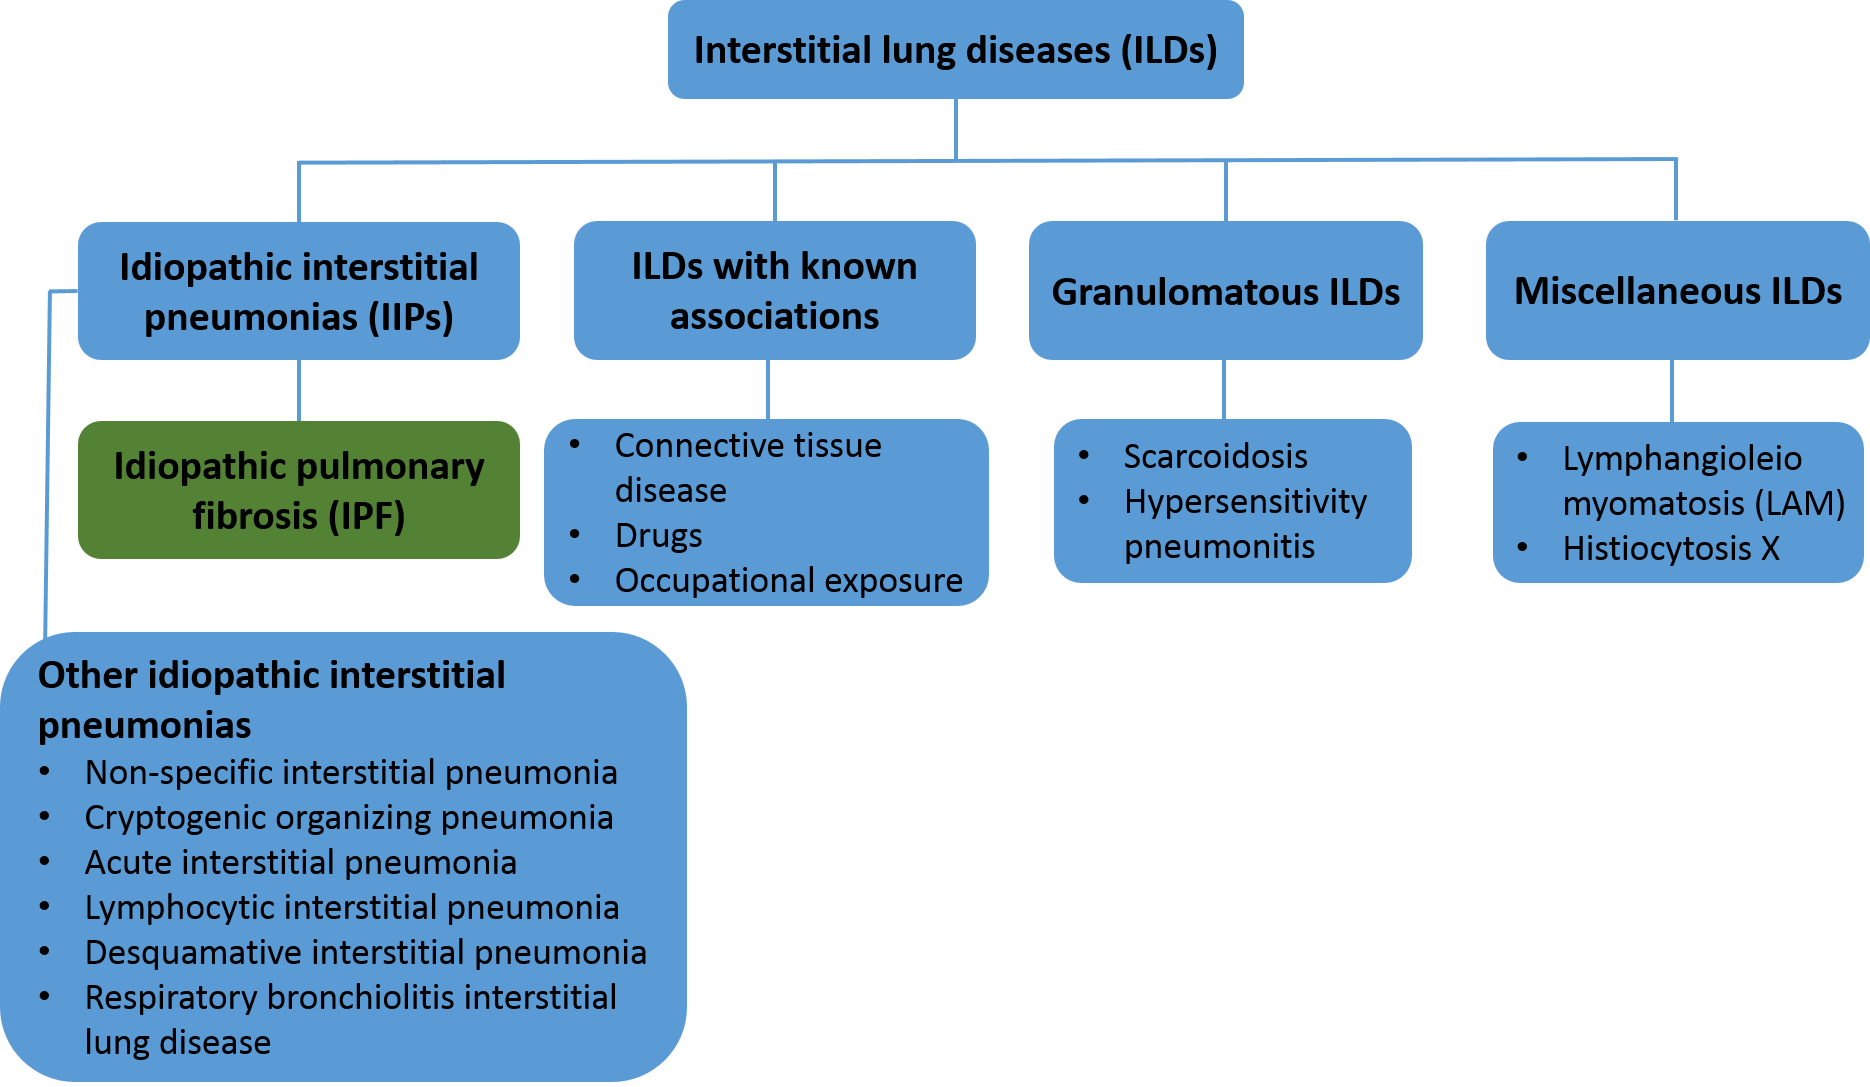
\includegraphics[height=3.5in]{Background/Image/DiseaseClassification.png}
  \caption{Classification of the interstitial lung diseases. IPF belongs to the family of interstitial lung disease (ILD), and belongs to a subgroup known as idiopathic interstitial pneumonia (IIP) \citep{troy2012management}.}
  \label{fig:DiseaseClassification}
\end{figure*}

%%%%%%%%%%%%%%%%%%%%%%%%%%%%%%%%%%%%%%%%%%%%%%%%%%%%%%%%%%%%%%%%%%5
\section{Epidemiology, etiology and pathogenesis} 
\subsection{Epidemiology}
Although IPF is considered a rare disease, this disease is the most common form of IIP \citep{travis2013official}. The incidence of IPF is similar to that of stomach, brain, and testicular cancers and has recently been demonstrated to be rising over time \citep{richeldi2017idiopathic}. A cohort study including patients diagnosed with ILDs at Aarhus University Hospital showed that IPF was the most common diagnosis (28\%) followed by connective tissue disease-related ILD (14\%), hypersensitivity pneumonitis (7\%) and non-specific interstitial pneumonia (NSIP) (7\%) \citep{hyldgaard2014cohort}. Although there is little data available estimating worldwide incidence, a recent study showed that in Europe and North America, the prevalence of IPF is estimated to range between 2.8 and 18 cases per 100,000 people per year, and this value might be lower in Asia and South America, where it is estimated to range from 0.5 to 4.2 cases per 100,000 individuals per year \citep{richeldi2017idiopathic}. IPF is more likely to affect men than women, and is rare in people younger than 50 years \citep{raghu2011official, raghu2006incidence}. The incidence is estimated to be 13 cases/100,000 in women and 20 cases/100,000 in men \citep{xaubet2017idiopathic}. In addition, the incidence of IPF increases with age \citep{meltzer2008idiopathic}. The reason that incidence has increased in recent years is most likely because of improved diagnostic methods and increased life expectancy \citep{xaubet2017idiopathic}.

%%%%%%%%%%%%%%%%%%%%%%%%%%%%%%%%%5
\subsection{Pathogenesis and potential contributors to aetiology}
Historically, IPF was considered a chronic inflammatory disorder, which gradually progressed to established fibrosis \citep{richeldi2017idiopathic}. Now IPF is generally regarded as a consequence of multiple interacting factors, in which repetitive local micro-injuries to an ageing alveolar epithelium plays an important role \citep{richeldi2017idiopathic}. These micro-injuries initiate aberrant epithelial-fibroblast communication, the induction of matrix-producing myofibroblasts, and considerable extracellular matrix accumulation and remodelling of lung interstitium \citep{richeldi2017idiopathic}. Although the aetiology of IPF is unknown, currently,  environmental exposures and genetic factors have been supported by some researchers as providing important inducement \citep{taskar2006idiopathic,meltzer2008idiopathic,xaubet2017idiopathic,richeldi2017idiopathic}. In addition, \gls{ger}, exposure to silica, brass, steel and wood dust, livestock and agriculture work, and the construction of wooden houses are also potential risk factors for the pathogenesis of IPF \citep{taskar2006idiopathic,xaubet2017idiopathic}.

\subsubsection{Environmental exposures}
The relationship between environmental exposures and IPF has been consistently demonstrated by case studies. Asbestosis, for example, is a case in which environmental material is associated with pulmonary fibrosis \citep{meltzer2008idiopathic}. There are studies indicating that the pathogenesis and progression of IPF are influenced by particulate inhalation, which is supported by the fact that the development of IPF consistently relates to cigarette smoking history in most patients \citep{baumgartner1997cigarette,richeldi2017idiopathic}. Additionally, other environmental factors including metal and wood dusts, agriculture and farming, viruses, and stone and silica have also been proposed \citep{raghu2011official, taskar2006idiopathic}.

\newpage

\subsubsection{Genetic factors}
Increasing evidence indicates that genetic predisposition plays an essential part in the development of IPF \citep{xaubet2017idiopathic,richeldi2017idiopathic}. This evidence is based on the existence of familial forms of the disease, and it has been shown that around 2.2\% to 3\% of IPF cases are familial \citep{xaubet2017idiopathic}. The most likely mode of genetic transmission of pulmonary fibrosis in familial cases is autosomal-dominant with variable penetrance \citep{steele2005clinical,allam2006idiopathic,lee2005familial,musk1986genetic}. Rare genetic variants have been identified in cases where ILDs affect two or more members of the same biological family, including genes associated with alterations in host defence (MUC5B, ATP11A, TOLLIP), telomere maintenance (TERT, TERC, PARN, RTEL, OBFC1), surfactant dysfunction (SFTPC, SFTPA2) and epithelial barrier function (DSP, DPP9) \citep{alder2008short,raghu2011official,seibold2011common,xaubet2017idiopathic}. Among them, MUC5B, a promoter site of an airway mucin gene, is the most strongly associated with development of both familial and sporadic IPF \citep{richeldi2017idiopathic}. MUC5B encodes a mucin-5B precursor protein that contributes to airway mucous production and might have an important role in lung host defence. It has also been noted that members of the same biological family may be affected by different types of ILDs, such as non-specific interstitial pneumonia and cryptogenic organizing pneumonia \citep{xaubet2017idiopathic}.

%%%%%%%%%%%%%%%%%%%%%%%%%%%%%%%%%%5
\section{Diagnosis}
The diagnosis of IPF often requires a multidisciplinary discussion, involving pulmonologists, chest radiologists, and chest pathologists experienced in the field of ILDs \citep{flaherty2004idiopathic,king2011idiopathic,raghu2011official}. This multidisciplinary approach has been accepted in consensus guidelines all over the world and has helped to standardize IPF diagnosis \citep{raghu2011official,richeldi2017idiopathic}. Usually, IPF is diagnosed by identification of a pattern of UIP on the basis of radiological or histological criteria in patients without evidence of an alternative cause.  The biggest challenge of diagnosis for clinicians is how to exclude other idiopathic interstitial pneumonias, fibrotic nonspecific interstitial pneumonia, and interstitial lung disease associated with occupational or environmental exposure, connective tissue disease, and drugs \citep{king2011idiopathic,richeldi2017idiopathic}. This differential diagnosis is really important, since typical UIP is not exclusive to IPF, but may associate with some other conditions, such as chronic hypersensitivity pneumonitis and asbestosis. Many patients have a history of environmental exposures or medical treatments which clinicians need to take into consideration for diagnosis \citep{richeldi2017idiopathic}.

\subsection{Clinical presentations}
Patients with IPF usually suffer from unexplained progressive dyspnea on exertion and chronic dry cough, bibasilar inspiratory crackles, and finger clubbing. Bibasilar inspiratory crackles are heard on chest auscultation and finger clubbing is found in about 30\% of patients \citep{raghu2011official,king2011idiopathic,richeldi2017idiopathic}. Chest pain, fatigue, malaise, and weight loss are also typical symptoms for IPF patients \citep{douglas2000idiopathic, king2001predicting}. These clinical presentations might initially be attributed to ageing or some comorbidities such as cardiovascular disease, or obesity \citep{richeldi2017idiopathic}. Therefore, in order to avoid diagnostic delays, it is necessary for primary care physicians to have clinical suspicion of IPF. Some patients may present with acute respiratory exacerbations usually accompanied by fever and influenza-like symptoms within a few days or weeks from the first clinical symptom. In these cases, clinicians require careful diagnostic distinction from other forms of acute ILDs \citep{richeldi2017idiopathic}. Pulmonary function tests (PFTs) from IPF patients usually show a restricted pattern with low percent predicted \gls{tlc} and \gls{dlco}. But for some patients with early disease, PFT results might be normal or mildly abnormal \citep{douglas2000idiopathic,raghu2006incidence}.

\subsection{Radiographic features} \label{RadiographicFeatures}
HRCT of the chest has become an essential tool for the diagnosis of IPF, which is usually associated with identification of a UIP pattern. The presence of UIP pattern on HRCT is characterised by appearance of honeycombing cysts, reticular opacities and ground-glass abnormalities (Figure \ref{fig:RadiologicalImaging}) \citep{king2011idiopathic,raghu2011official,richeldi2017idiopathic}. Honeycombing is common, and essential for a definite diagnosis \citep{raghu2011official}. On HRCT, honeycombing is presented as clustered cystic airspaces with a typical diameter of 3-10 mm but occasionally as large as 2.5 cm, and in a predominantly subpleural and posterior basal distribution \citep{hansell2008fleischner,richeldi2017idiopathic}. Reticular opacities are often associated with traction bronchiectasis \citep{nishimura1992usual, johkoh1999idiopathic}. Ground-glass is a common characteristic of UIP pattern, although it is sometimes less extensive than reticular. The distribution of abnormalities are often basal, peripheral and patchy \citep{raghu2011official}. If patients show micronodules, air-trapping, non-honeycomb cysts, extensive ground glass opacities, consolidation, or a peribronchovascular-predominant distribution, alternative diagnosis should be taken into account \citep{hwang2009computed, souza2006idiopathic}. If patients show reticular abnormalities located in subpleural and basal regions, but no honeycombing appearance, possible UIP patterns should be taken into consideration, then a surgical lung biopsy is suggested to make a definite diagnosis \citep{raghu2011official,richeldi2017idiopathic}. 

\begin{figure}[H]
  \centering 
  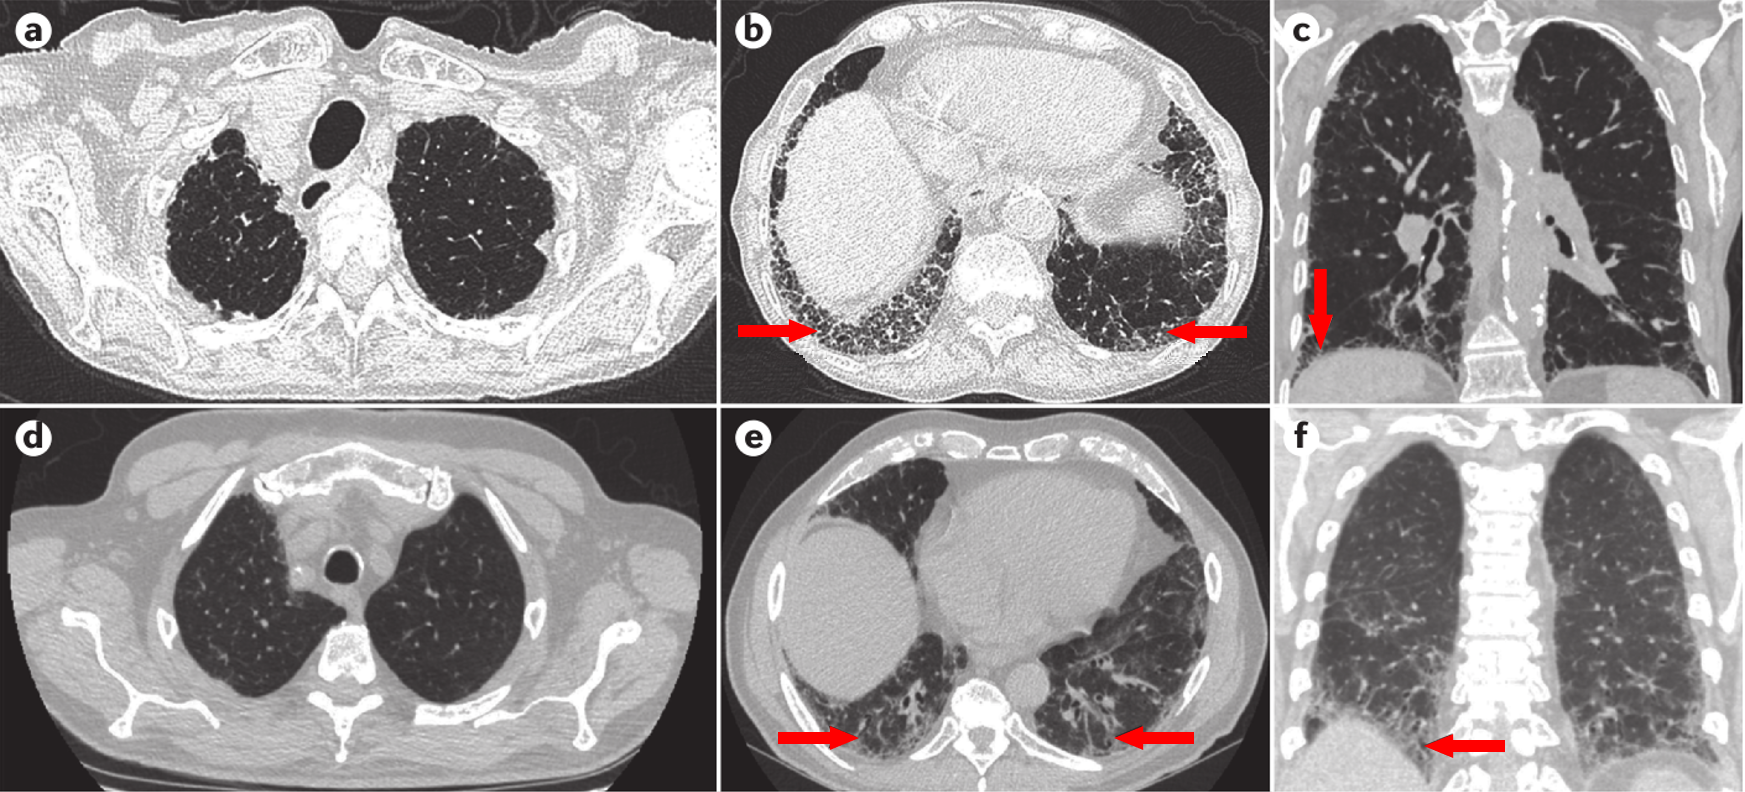
\includegraphics[height=2.5in]{Background/Image/RadiologicalImaging.png}
  \caption{HRCT images of UIP pattern from two patients. The first is from a woman with progressive cough and dyspnoea, showing her upper (a), lower (b) lung zones and a sagittal plane of the lungs (c). These images show lower lobe-predominant peripheral honeycomb change (b and c, arrows), which is typical of UIP pattern. This patient had no systemic disease or exposures that would exclude idiopathic disease: the diagnosis of IPF is certain. In contrast, the second is a woman with progressive breathlessness, who could be diagnosed with possible IPF. The upper (d), lower (e) lung zones and sagittal image of the lungs (f) demonstrate peripheral, basilar-predominant, reticular densities with traction bronchiectasis (e and f, arrows) consistent with fibrosis. Surgical lung biopsy is suggested. Reproduced from \citep{martinez2017idiopathic}.}
  \label{fig:RadiologicalImaging}
\end{figure}


\subsection{Histopathology}
When HRCT features are not enough for a certain diagnosis of IPF, surgical lung biopsy is suggested \citep{richeldi2017idiopathic}. The main histopathologic hallmarks of UIP pattern is characterized by a heterogeneous appearance, best seen at low magnification, with areas of subpleural fibrosis and honeycomb (i.e. cystic fibrotic airspaces lined by bronchiolar epithelium and often filled by mucin and variable numbers of inflammatory cells), alternating with areas of less affected or normal parenchyma \citep{ american2000idiopathic, travis2002american} (Figure \ref{fig:SurgicalLungBiopsy}). Small areas of active fibrosis (fibroblast foci) are present in the background of collagen deposition, and they reflect the temporal heterogeneity and indicate current ongoing disease \citep{king2011idiopathic}. Another feature of UIP pattern is that the inflammation is often absent or mild and consists of a patchy interstitial infiltrate of lymphocytes and plasma cells \citep{raghu2011official,king2011idiopathic}. Although surgical lung biopsy is essential for a correct diagnosis, careful consideration is required for every patient to estimate whether the risks of surgical lung biopsy outweigh the potential benefits of the histopathologic information. For older patients with comorbidities or clinically significant physiological impairment, it is suggested to avoid surgical lung biopsy \citep{richeldi2017idiopathic}.

\begin{figure}[htbp]
  \centering 
  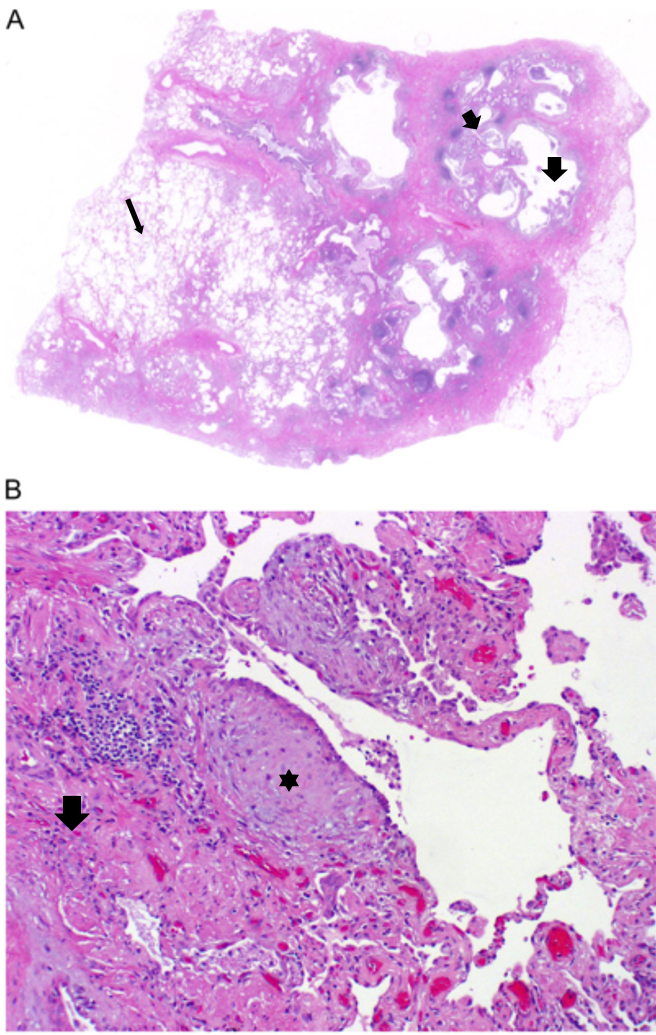
\includegraphics[height=2.9in]{Background/Image/SurgicalLungBiopsy.png}
  \caption{ Surgical lung biopsy specimens of UIP pattern. (A) Scanning power microscopy showing a patchy process with honeycomb
spaces (thick arrow), some preserved lung tissue regions (thin arrow), and fibrosis extending into the lung from the subpleural regions. (B) Adjacent to the regions of more chronic fibrosis (arrow) is a fibroblast focus (asterisk), recognized by its convex shape and composition of edematous fibroblastic tissue, suggestive of recent lung injury. Reproduced from \citep{raghu2011official}.}
  \label{fig:SurgicalLungBiopsy}
\end{figure}

\subsection{Diagnostic criteria} \label{DiagnosisCriteria}
''Gold standard'' diagnostic criteria for IPF have been developed by the \gls{ats} and the \gls{ers} in a statement of published guidelines \citep{raghu2011official}. These criteria are:
\begin{enumerate}
  \item Exclusion of other known causes of ILD (e.g. domestic and occupational environmental exposures, connective tissue disease, and drug toxicity).
  \item The presence of a UIP pattern on HRCT in patients not subjected to surgical lung biopsy.
  \item Specific combinations of HRCT and surgical lung biopsy pattern in patients subjected to surgical lung biopsy.
\end{enumerate}

Beyond that, minor criteria have also been set for the diagnosis of IPF in the absence of a surgical lung biopsy \citep{raghu2011official}:
\begin{enumerate}
  \item Age $>$ 50 years.
	\item Insidious onset of otherwise unexplained dyspnea on exertion.
	\item Duration of illness being over 3 months.
	\item Bibasilar inspiratory crackles (dry or ''Velcro'' type).
\end{enumerate}

Figure \ref{fig:IPFDiagnosis} shows the diagnostic workflow for adult patients with ILD and suspected IPF. If the high-quality HRCT evidence is sufficient enough for the recognition of histopathologic UIP pattern, surgical lung biopsy is not essential \citep{hunninghake2001utility, raghu1999accuracy, flaherty2003radiological, quadrelli2010radiological}. However, a multidisciplinary discussion among experienced clinical, radiologic and histopathologic experts is particularly important when the radiologic and histopathologic patterns are discordant (e.g., HRCT is inconsistent with UIP and histopathology suggests UIP) \citep{raghu2011official}. Radiologic or pathologic UIP pattern is not 100\% specific to IPF \citep{lynch2006usual, trahan2008role, silva2008chronic}.

\begin{figure}[htbp]
  \centering 
  
\includegraphics[height=3.5in]{Background/Image/IPFDiagnosis.png}
  \caption{Diagnostic algorithm for IPF. Patients with suspected IPF (i.e., patients with unexplained dyspnea on exertion and/or cough with evidence of ILD) should be carefully evaluated for identifiable causes of ILD. In the absence of an identifiable cause for ILD, an HRCT demonstrating UIP pattern is diagnostic of IPF. In the absence of UIP pattern on HRCT, IPF can be diagnosed by the combination of specific HRCT and histopathological patterns. The accuracy of the diagnosis of IPF increases with multidisciplinary discussion (MDD) among ILD experts. Reproduced from \citep{raghu2011official}.}
  \label{fig:IPFDiagnosis}
\end{figure}

%%%%%%%%%%%%%%%%%%%%%%%%%%%%%%%%%%%%
\section{Clinical course} 

Some studies indicate that IPF patients have median survival time between two and three years from the time of diagnosis \citep{bjoraker1998prognostic, flaherty2002clinical, nicholson2000prognostic, rudd2007british, king2001idiopathic, king2011idiopathic}. For most IPF patients, the clinical course has been described as a general decline in pulmonary function until eventual death from respiratory failure or complicating comorbidity \citep{carrington1978natural, tukiainen1983prognosis, gross2001idiopathic}, however, the individual disease progression can be highly variable \citep{kim2006classification,meltzer2008idiopathic}. It appears that there are several possible clinical courses for patients with IPF (shown in Figure \ref{fig:IPFDiseaseProgression}) \citep{raghu1987idiopathic}: slow and gradual progression over many years (the most common) \citep{ryu2014idiopathic,meltzer2008idiopathic,raghu2011official}; rapid and accelerated decline \citep{kim2006classification,selman2007accelerated}; and acute exacerbations \citep{king2011idiopathic,xaubet2017idiopathic}. It is difficult to predict the natural history of disease progression for a given patient at the time of the diagnosis \citep{raghu2011official}. Whether the different clinical courses are influenced by geographic, ethnic, cultural, racial, or other factors remains unknown. But some evidence has been suggested that worsening prognosis may be associated with older people ($>$ 70 years old), smoking history, low body mass index (BMI), severe physiological impairment, and large radiological extent of disease \citep{ley2011clinical}. Other comorbidities such as emphysema and pulmonary hypertension may also have an impact on the disease course \citep{mejia2009idiopathic, wells2003idiopathic, lettieri2006prevalence}. While prediction of the likely course of disease is currently not possible, it would be very beneficial to enable clinicians to make an appropriate and optimal treatment plan as early as possible.
\newpage

\subsection{Slow and rapid progressive course}
Most IPF patients deteriorate relatively slowly, and their pulmonary function usually decreases gradually over months to years after the first clinical symptoms (cough and progressive dyspnoea) \citep{ryu2014idiopathic,meltzer2008idiopathic,raghu2011official}. Patients usually experience reduction of lung volumes, and hypoxaemia at rest that worsens with exercise. This is accompanied by a decline of \gls{fvc}  by a mean of 0.13 L to 0.21 L per year \citep{ley2011clinical}. In contrast, a subgroup of patients with IPF, mainly male cigarette smokers, experience a rapid worsening of symptoms, and insufficiency of pulmonary function \citep{kim2006classification, king2011idiopathic}, known as accelerated IPF. The patients with rapid progression have reduced survival time relative to those with a slowly progressive clinical course.

\subsection{Acute exacerbations of IPF}
“Acute exacerbation” was first proposed by Japanese physicians to describe acute, unexpected worsening of respiratory functions and severe hypoxaemia in patients with IPF, without a clear trigger \citep{kondoh1993acute, gross1962concept}. The rapid deterioration occurs in a small minority of patients with IPF (about 5-10\%), with absence of infection, heart failure, pneumothorax, or pulmonary embolism \citep{azuma2005double,king2011idiopathic,raghu2011official}. The prognosis for patients with acute exacerbations is poor, and it may happen at any stage in the course of IPF \citep{kim2006acute,parambil2005histopathologic,sakamoto2009acute,kondoh2010prognostic}. Patients with acute exacerbation usually experience poor respiratory decline, worsened cough, fever and increased sputum production \citep{ambrosini2003acute,kim2006acute}. The mortality rate for patients with acute exacerbations is over 60\% \citep{wootton2011viral, lettieri2006prevalence}; for cases requiring mechanical ventilation, the mortality is close to 100\% \citep{king2011idiopathic,xaubet2017idiopathic}.

\begin{figure}[htbp]
  \centering 
  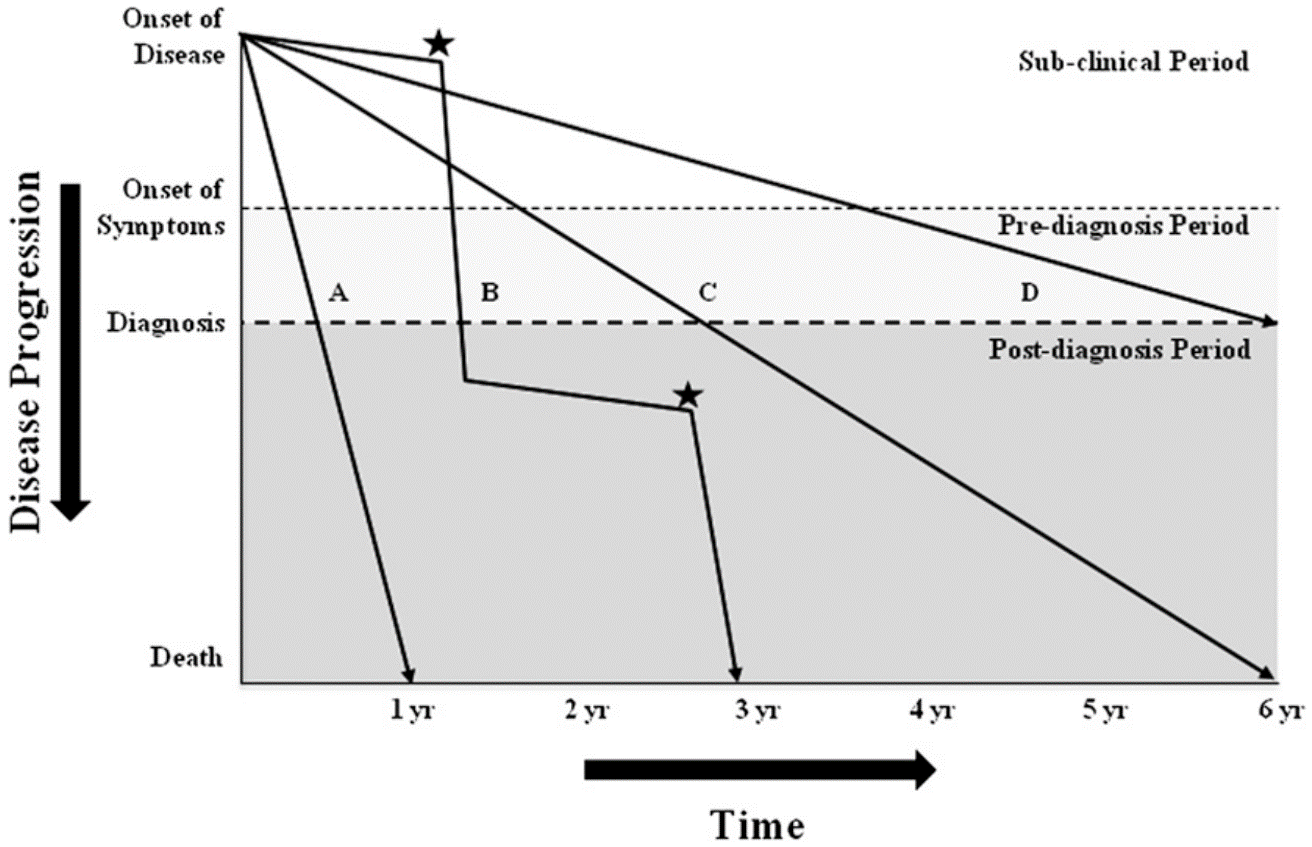
\includegraphics[height=3.2in]{Background/Image/IPFDiseaseProgression.png}
  \caption{Schematic representation of potential clinical courses of IPF.  A sub-clinical period of disease progression exists during which only radiographic evidence of disease may be noted. This is followed by a symptomatic phase comprising clinical stages (both pre-diagnosis and post-diagnosis). The rate of deterioration and progression to death may be fast (line A), mixed (line B), or slow (lines C and D), with phases of relative disease stability interspersed with acute decline (asterisks). Reproduced from \citep{ley2011clinical}.}
  \label{fig:IPFDiseaseProgression}
\end{figure}

%%%%%%%%%%%%%%%%%%%%%%%%%%%%%%%%%%%5
\section{Complications and comorbidities}
%For the purposes of diagnoses, a complication is a condition that arises during the hospital stay, and a comorbidity is a pre-existing condition that affects the treatment received. 
Complications and comorbidities can occur in patients with IPF that may influence the clinical course and prognosis \citep{xaubet2017idiopathic,king2017idiopathic,martinez2017idiopathic}. It is reported that only 12\% of patients with IPF have no comorbid illness, and most patients have comorbidities \citep{raghu2011official, kim2015natural, harari2016epidemiology, kreuter2016impact}. Emphysema and pulmonary hypertension are both important comorbid conditions in IPF patients \citep{raghu2015comorbidities,martinez2017idiopathic}, and are briefly outlined here.

\subsection{IPF and emphysema}

Several research groups have described a syndrome in which IPF coexists with pulmonary emphysema \citep{wells1997lone, wells2003idiopathic, cottin2005combined,meltzer2008idiopathic}. In 2005, \cite{cottin2005combined} presented a syndrome named \gls{cpfe}. Both IPF and emphysema are associated with a significant smoking history, and CPFE is strongly associated with exercise hypoxaemia, severe dyspnea on exertion, upper lobe emphysema and lower lobe fibrosis, unexpected subnormal lung volumes, and severe reduction of carbon monoxide transfer \citep{silva2008idiopathic,mejia2009idiopathic,cottin2010pulmonary,king2011idiopathic,lin2015combined}. Currently, whether CPFE is a distinct clinical entity or not remains unknown, i.e. whether this is just the presence of two different diseases running in parallel is unclear \citep{king2011idiopathic,lin2015combined}. Some researchers suggest that CPFE should be regarded as a distinct clinical entity, since it has a characteristic pulmonary function feature and unique natural history that is different from pure emphysema or IPF alone \citep{cottin2005combined, lin2015combined, xaubet2017idiopathic}. CPFE occurs more frequently in males than in females and its prevalence is about 30\% to 47\% in patients with IPF \citep{xaubet2017idiopathic}. It is often associated with a significant drop of DLCO and severe hypoxaemia during exercise due to the additive effect of emphysema and fibrosis \citep{xaubet2017idiopathic}. 
\newpage

\begin{figure}[htbp]
  \centering 
  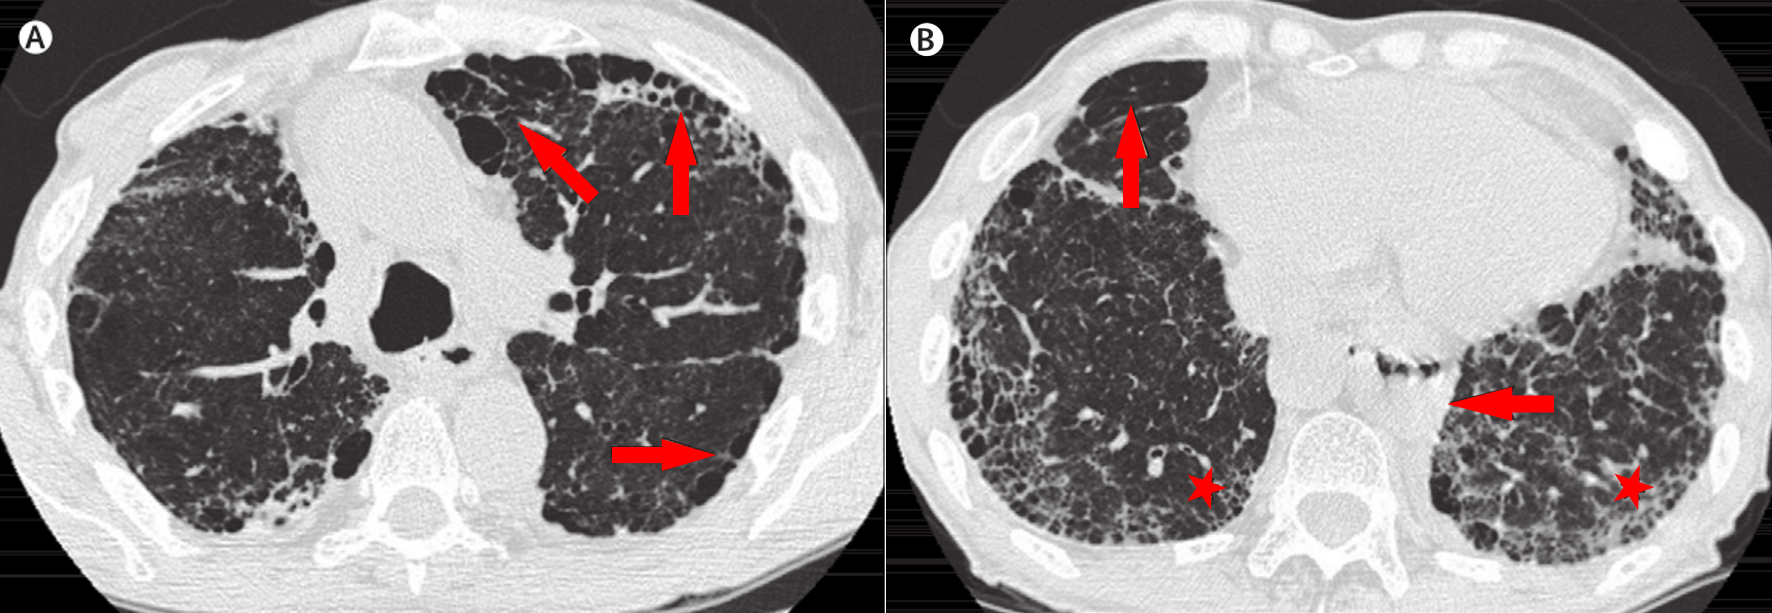
\includegraphics[height=2.05in]{Background/Image/CPFEImaging.png}
  \caption{ Combined pulmonary fibrosis and emphysema. High-resolution CT shows emphysematous lesions (arrows) in the upper lobes (in Figure A), emphysema (arrow) and usual interstitial pneumonia-like lesions (stars) in the lower lobes (in Figure B). Reproduced from \citep{king2011idiopathic}.}
  \label{fig:CPFEImaging}
\end{figure}

\subsection{IPF and pulmonary hypertension}
Pulmonary hypertension (PH), defined as a mean pulmonary artery pressure of $>$ 25 mmHg at rest, is a frequent form of comorbid condition in patients with IPF and is the main determinant of poor prognosis \citep{raghu2011official, xaubet2017idiopathic}. It is estimated that the incidence of pulmonary hypertension is around 30\% to 50\% in IPF patients \citep{king2017idiopathic}. In general, pulmonary hypertension occurs due to several factors, with chronic hypoxia-induced vasoconstriction and destruction of the pulmonary capillary bed induced by fibrosis being the two main causes \citep{hayes2016influence}. The presence and development of pulmonary hypertension is associated with significant dyspnea, functional impairment (particularly in DLCO) and decreased exercise capacity, and may increase risk of mortality for patients with IPF \citep{mejia2009idiopathic,lettieri2006prevalence,nadrous2005impact}. Some studies have shown that combined pulmonary fibrosis and pulmonary hypertension has a significantly negative effect on the survival in patients with IPF alone, probably caused by the increased pulmonary vascular resistance \citep{raghu2011official, king2011idiopathic}. Currently, whether IPF with pulmonary hypertension represents a distinct  clinical entity (IPF–PH) is still unclear \citep{raghu2011official}.

%%%%%%%%%%%%%%%%%%%%%%%%%%%%%%%%%%%%%%%%%5
\section{Physiological alterations}
The clinical presentation of IPF is related to a number of physiological alterations of the lung \citep{crystal1976idiopathic, plantier2018physiology}. These alterations have a complex and negative impact on all compartments of the respiratory system, from lung volume and compliance to gas exchange, from conducting airways to lung vasculature \citep{plantier2018physiology}. In general, patients with IPF usually have reduced lung volumes, reduced lung compliance, reduced diffusing capacity, increased \gls{fev1/fvc}, and arterial hypoxaemia that worsens with exercise \citep{crystal1976idiopathic,american2000idiopathic,cortes2014idiopathic,plantier2018physiology}. These alterations in lung physiology are summarized in Table \ref{tab:IPFPhysiologicAlterations}.

\begin{table}[htbp]
\centering
\caption{Alterations of lung function tests in \gls{ipf} Reproduced from \citep{plantier2018physiology}}
\label{tab:IPFPhysiologicAlterations}
\begin{tabular}{l c c}
\hline
  & \bf{Mild IPF} & \bf{Moderate to severe IPF} \\ 
\hline
\bf{Static lung volumes} &  &  \\
- TLC & Normal & Decreased\\
- FRC & Normal & Decreased\\
\hline
\bf{Spirometry} &  &  \\
- FVC & Normal & Decreased\\
- FE$V_1$/FVC & Normal or increased & Normal or increased\\
\hline
\bf{Airways} &  &  \\
- Cough reflex & Increased & Increased\\
- Airway resistance & Decreased & Decreased\\
\hline
\bf{Blood gases at rest} &  &  \\
- $P_aO_2$ & Normal & Decreased\\
- $P_aCO_2$ & Normal & Decreased\\
\hline
\bf{Carbon monoxide transfer} &  &  \\
- DLCO & Decreased & Decreased\\
- $V_A$ & May be normal & Decreased\\
- $K_{CO}$ & May be normal & Decreased\\
\hline
\bf{Exercise physiology} &  &  \\
- Peak $V_{O_2}$ & May be normal & Decreased\\
- $V_D/V_T$ & Increased & Increased\\
- $V_E/V_{CO_2}$ & Increased & Increased\\
- PAP at exercise & Increased & Increased\\
- $P_{A-a} O_2$ at exercise & Increased & Increased\\
\hline
\bf{Pulmonary haemodynamics at rest} &  &  \\
- PAP & May be increased & Frequently increased\\
- PCWP & Normal & May be increased\\
\hline
\end{tabular}
\begin{tablenotes}
        \footnotesize
        \item{FVC: forced vital capacity; FE$V_1$ : forced expiratory volume in 1 s; TLC: total lung capacity; FRC: functional residual capacity; $P_aO_2$ : arterial oxygen tension; $P_aCO_2$ : arterial carbon dioxide tension; DLCO : diffusing capacity of the lung for carbon monoxide; $V_A$ : alveolar volume; $K_CO$ : transfer constant of carbon monoxide; PAP: pulmonary artery pressure; PCWP: pulmonary capillary wedge pressure; $V_{O_2}$ : oxygen uptake; $V_D/V_T$ : ratio of dead space volume to tidal volume; $V_E/V_{CO_2}$ : ratio of minute ventilation to carbon dioxide elimination; $P_{A-a} O_2$ : alveolar–arterial oxygen tension difference.}
\end{tablenotes}
\end{table}

\subsection{Alterations in the mechanical properties of the lung} \label{MechanicalAlteration}
\subsubsection{Reduction in lung compliance}
IPF disease often results in reduction in lung compliance (i.e. an increase in lung tissue stiffness). Studies have shown that the reduced lung compliance is caused by a reduction in the compliance of the lung extracellular matrix and by alterations in pulmonary surfactant \citep{plantier2018physiology}. In patients with IPF, surfactant shows alterations in its lipid profile \citep{gunther1999surfactant, schmidt2002altered}, which leads to severely impaired surface activity \citep{gunther1999surfactant}. The reduction in lung compliance may happen from an early stage of IPF \citep{plantier2018physiology}. A study of 31 IPF patients from \citep{zielonka2010angiogenic} showed that the static lung compliance was consistently and significantly reduced (by 44 $\pm$ 6\%). A similar result was found by in another study \citep{orens1995sensitivity}, where all of the measured IPF patients had abnormal static lung compliance, which suggests that measurement of lung compliance could help with the early diagnosis of IPF.

The alterations of lung compliance in IPF patients appear to be strongly correlated with the degree of lung fibrosis as assessed by scoring of lung biopsies \citep{fulmer1979morphologic,plantier2018physiology}. \cite{nava1999lung} measured the dynamic lung compliance in seven patients with end-stage IPF, which showed that the reduction in lung compliance may be correlated with the progress of the disease. Currently, whether the reductions in lung compliance relate to clinical presentations (e.g. dyspnoea) remains unclear, but it is highly likely that the lung compliance has a strong relationship with the respiratory muscles and thus has an impact on the work of breathing \citep{plantier2018physiology}. In addition, as the distribution of disease is heterogeneous in IPF lungs, lung compliance is expected to be uneven between different lung regions \citep{organ2015structural}, but more evidence is needed to understand the implications of disease distribution outcomes.

\subsubsection{Reduction of lung volumes}
The restriction of lung volumes (total lung capacity (TLC), \gls{frc}, forced vital capacity (FVC), and \gls{rv}) is typical in patients with IPF. This restriction of lung volumes often occurs at some time point in the clinical course of IPF \citep{american2000idiopathic, plantier2018physiology}. However, sometimes lung volumes may be normal in the early stage of IPF, especially for patients with superimposed chronic obstructive pulmonary disease \citep{martinez2006pulmonary}. \cite{cherniack1995correlation} studied 96 patients with biopsy-confirmed IPF. The range of TLC was from 42\% to 125\% predicted and the range of FVC was from 26\% to 112\% predicted. A reduction in lung volumes consistently relates to an increased risk of death \citep{martinez2006pulmonary}, and is weakly associated with dyspnoea or quality of life \citep{du2011ascertainment}. However, whether the reduced lung volumes reflects the disease progression of IPF is still unknown \citep{plantier2018physiology}. Interestingly, patients with CPFE have higher RV and TLC compared to the patients with IPF alone \citep{mura2006presence}, which may be caused by the effects of comorbid pulmonary emphysema on lung compliance \citep{doherty1997cryptogenic}.

\subsubsection{Alterations in the conducting airways}
Some evidence suggests that alterations also occur in conducting airways in patients with IPF, including increased airway epithelial cell proliferation \citep{vuorinen2008peroxiredoxin} and differentiation \citep{plantier2016increased}, and increased numbers of visible bronchioles in the distal regions \citep{chilosi2002abnormal}. A reduction in conducting airway resistance was found in IPF lungs compared with normal, which may contribute to an increased ratio of FE$V_1$ to FVC \citep{pastre2015different}. \cite{plantier2016increased} used volumetric capnography to estimate the volume of conducting airways in patients with IPF, patients with other ILDs, and healthy people. The results showed that conducting airway volume was significantly higher in IPF lungs in comparison with non-IPF ILD lungs and healthy lungs. However, this change in airway volume was not associated with the severity of alveolar lesions, dyspnea, cough or quality of life \citep{plantier2016increased}. The increase in airway volume in IPF may reflect dilation of airways consistent with bronchiectasis that can be characteristic of this disease, and a commonly accepted view is that bronchiectasis in IPF may be caused by fibrotic retraction of peribronchiolar alveolar attachments and subsequent airway dilation \citep{sumikawa2008computed}. However, a recent study found that bronchiectasis had a weak relationship with total fibrosis extent observed from CT imaging \citep{walsh2015relationship}, which means the remodelling of conducting airways in IPF may be dissociated from alveolar fibrosis \citep{plantier2016increased}. Patients with IPF usually have more rapid breaths with the progression of disease \citep{kornbluth1980respiratory, renzi1982pattern}, and have a relatively increased flow rate in the conducting airways due to the increased static elastic recoil \citep{american2000idiopathic}. Additionally, it has been suggested that at least part of the ventilation abnormalities seen in IPF is associated with small airways disease with peribronchiolar fibrosis and inflammation, and 70\% of IPF patients have narrowed small airways \citep{crystal1976idiopathic}.

\subsubsection{Alterations in the lung vasculature} \label{VasculatureAlterations}
Vascular lesions are observed in the pulmonary vasculature in patients with IPF, and often lead to disproportionate increases in the pulmonary vascular resistance and pulmonary hypertension \citep{plantier2018physiology}. The tissues adjacent to the areas of fibrosis have been shown to have an increase in vessel profusion, whereas the fibrotic tissue itself demonstrates a reduced number of blood vessels \citep{cosgrove2004pigment,ebina2004heterogeneous}. \cite{Jacob2016Evaluation} explored the relationship between \gls{pvv} and ILD extent (includes ground glass, reticular and honeycomb patterns). It was found that PVV had a strong relationship with ILD extent ($R^2 = 0.73$, $P < 0.0001$) when using linear regression analysis. Furthermore, PVV was demonstrated to be an independent predictor of mortality, and a stronger predictor of mortality than all the other traditional CT features and pulmonary functional variables \citep{Jacob2016Evaluation}. The increase in PVV seen in more advanced fibrosis may be caused by the vascular capacitance of spared lung (the upper and middle lobes in patients with IPF, which is a predominantly basal disease), and may also relate to the increased negative intrathoracic pressure which non-compliant fibrotic lungs need to generate during inspiration \citep{Jacob2016Mortality}.

\subsection{Alterations in pulmonary gas exchange}
IPF is associated with multiple pathophysiological changes in pulmonary gas exchange. The lesions of the alveolar-capillary membrane in IPF lungs will impair both the diffusion capacity and ventilation/perfusion (V/Q) relationship, increase dead space ventilation and alveolar-arterial oxygen tension difference ($P_{A-a}O_2$), and finally cause chronic arterial hypoxaemia \citep{crystal1976idiopathic,plantier2018physiology,american2000idiopathic}.

\subsubsection{Reduced diffusing capacity of the lung}
The diffusing capacity of oxygen is considered to be reduced in almost all patients with IPF. However, in clinical examination, this diffusing capacity is technically very difficult to measure. Therefore, clinical tests actually measure the diffusing capacity of carbon monoxide (DLCO) which provides an estimate of the gas-exchange function of the whole lungs \citep{plantier2018physiology}. DLCO is a measure of the conductance of gas transfer from inspired gas to the red blood cells, and is usually tested in a single breath where the partial pressure difference between inspired and expired carbon monoxide is recorded \citep{rosenberg19961995,plantier2018physiology}. The \gls{kco} is an index of the efficiency of alveolar transfer of carbon monoxide. It can be referred to as DLCO/VA, where VA is the alveolar volume where gas exchange takes place \citep{graham20172017}.

It has been shown that DLCO is reduced compared with normal values in 98\% of IPF patients at initial diagnosis, although 27\% of patients have normal TLC volumes, and 56\% have normal FVC \citep{cortes2014idiopathic}. Interestingly, KCO is within the normal range in up to 30\% of IPF patients \citep{wallaert2012we}, particularly in patients with moderately reduced DLCO \citep{pastre2015different}. But a normal KCO value in IPF patients does not mean that pulmonary gas exchange is normal \citep{plantier2018physiology}. It has been noted that both DLCO and KCO are significantly associated with the degree of IPF measured from CT scans \citep{wells1997lone}, but DLCO correlates more strongly with exertional increases in $P_{A-a}O_2$ \citep{agusti1994clinical} and highly relates to both dyspnoea \citep{swigris2012ucsd} and survival time \citep{hamada2007significance}.

\subsubsection{Dead space ventilation}
Increased physiologic dead space ventilation (increased ratio of dead space volume to tidal volume $\mathrm{V_D}/V_T$) is an important characteristic of lungs with fibrosis and happens in most IPF patients both at rest and at exercise \citep{fulmer1976diffuse, crystal1976idiopathic, agusti1991mechanisms, miki2009acidosis}. The increased dead space is mainly caused by two physiologic features: the first is the increased anatomical dead space, which is a result of the dilation of conducting airways in IPF as discussed in Section \ref{MechanicalAlteration} \citep{plantier2016increased}; the second is the regional ventilation-perfusion mismatch (increased variation in regional ventilation-perfusion ratio, V/Q), which increases the physiologic dead space. In IPF lungs, the fibrotic (i.e. honeycomb or reticular) areas that are  not perfused or poorly perfused but still receive ventilation will have an increased regional V/Q ratio \citep{strickland1993cause, plantier2018physiology}. An early paper indicated that patients with IPF will often have a $\mathrm{V_D}/V_T$ ratio of greater than 0.4 compared with a normal person (approximate 0.3 for normal) \citep{crystal1976idiopathic}. In normal individuals the efficiency of ventilation improves with exercise (that is the VD/VT falls) \citep{ jones1966physiological, wasserman1975exercise}, but in more than 90\% of IPF patients $\mathrm{V_D}/V_T$ stays constant or may increase \citep{crystal1976idiopathic}. 

\subsubsection{Ventilation-perfusion mismatching}

It is generally thought that the hypoxemia of IPF is related to V/Q mismatching \citep{wagner1976distribution,crystal1976idiopathic,american2000idiopathic}. This V/Q mismatching may be associated with abnormalities both in ventilation and perfusion \citep{crystal1976idiopathic,strickland1993cause}. \cite{crystal1976idiopathic} showed an equilibrium picture of 127 Xe distribution, which was used to determine regional ventilation, and showed that patients with IPF have patchy, non-segmental areas of decreased ventilation where airway obstruction or alveolar destruction occurred. As for perfusion, a shift of perfusion was observed to the upper lobes (reflecting pulmonary hypertension) due to the basal distribution of fibrotic lesions, so that areas of relatively low V/Q ratios mostly presented in the upper zones of the lung \citep{crystal1976idiopathic}. However, \cite{strickland1993cause} indicated that the CT based cystic air spaces (i.e. honeycomb) were observed as poorly perfused (probably due to vascular obliteration) but were usually  normally ventilated, which explains the increase in physiologic dead space seen at rest and with exercise. Thus, a higher V/Q ratio can be seen in areas where fibrosis and cystic air spaces are dominant, which could be used to distinguish IPF from emphysema \citep{strickland1993cause}. In addition, an increased minute ventilation was found in most patients with IPF during exercise. This is mainly due to the increased respiratory frequency, and in part relates to an increase in dead space ventilation \citep{american2000idiopathic}.

\subsubsection{Arterial hypoxaemia}
Alterations in the mechanical properties of the lungs, impairment of diffusion capacity and ventilation-perfusion mismatch will finally lead to early-onset exertional chronic arterial hypoxaemia and later-onset resting chronic arterial hypoxaemia in IPF \citep{hempleman1991estimating, hughes1991dlco, plantier2018physiology}. Some studies support that the major cause of arterial hypoxaemia in a large proportion of IPF patients is not the diffusion barrier to oxygen or the anatomic shunts, as was originally suspected, but is due to ventilation-perfusion mismatching \citep{ finley1962cause, wagner1976distribution, american2000idiopathic}. The alveolar-arterial oxygen gradient ($P_{A-a}O_2$), which is calculated from arterial oxygen tension ($P_{a}O_2$) and alveolar oxygen tension ($P_{A}O_2$) may increase, resulting from the reduced ventilation-perfusion ratio, right-to-left shunting, or impairment of oxygen diffusion \citep{plantier2018physiology}. The increase in $P_{A-a}O_2$ reflects hypoxaemia in IPF \citep{agusti1991mechanisms}. In a study of 29 IPF patients, the measured average resting $P_a O_2$ was 69.3 mmHg, and four patients had normal resting $P_{a}O_2$. However, although the resting $P_{a}O_2$ can be normal in some IPF patients, the resting $P_{A-a}O_2$ is invariably abnormal (in about 97\% of the patients with IPF) \citep{crystal1976idiopathic}.

%%%%%%%%%%%%%%%%%%%%%%%%%%%%%%%%5
\section{Summary}
IPF is a devastating lung disease characterized by an irreversible decline of lung function, and its incidence increases with years of age. The current efforts of studies in IPF mostly focus on the  accurate identification and diagnosis of early IPF, underlying mechanisms of pathogenesis and potential bio-markers that can indicate the patient-specific clinical course. The presence of IPF is variable in most patients, but some common characteristics and progressions can be summarized, although this is challenging. The clinical and physiological features of IPF reviewed in this chapter provides background information for further quantitative analysis (Chapter 4) and computational modelling of patients with IPF (Chapter 5). 

% \chapter{Pulmonary lobar segmentation from CT scans} \label{Yuwen_Segmentation}
Identification of pulmonary lobes is of great importance for image-based analysis of lung function and disease progression. Segmentation of lobes can facilitate intra-patient image registration for localizing and tracking fibrosis disease progression over time, since lobes are important structural landmarks \citep{lassen2011interactive}. Also, knowing the lobar distribution of pulmonary fibrosis disease is helpful to understand the pathophysiology of the disease and to guide a patient-specific functional simulation.  However, the pulmonary lobar fissure is usually difficult to segment fully automatically, especially for diseased lungs, as fissures are thin, usually of fuzzy appearance and incomplete, and can be obscured by or confused with features of disease \citep{ukil2009anatomy}. The following chapter outlines the development of an automatic pulmonary lobar segmentation method using a statistical finite element shape model of the lungs and lobar fissures to guide segmentation. Unlike 'deep learning' methods, this approach requires relatively few subject images as a training set. Development of this method was motivated by the poor reliability of existing methods for a guaranteed estimate of fissure location, particularly in volumetric images of IPF, or when only thin-slice CT (non-volumetric images) are available.

%% Section 1
\section{Background} \label{SegmentationBackground}
\subsection{Pulmonary lobar anatomy}
Within the thorax, the lungs are enclosed by the ribs, and the base of the lungs rests on the diaphragm. The space in between the two lungs is called the mediastinum, and contains the heart, major blood vessels, the esophagus, the trachea, main bronchi, and several other thoracic structures. The airways, blood vessels and nerves enter the lungs from the mediastinum at the hilum. The lungs themselves comprise airways, vessels and a connective tissue framework referred to as the interstitium.

Human lungs are divided into five distinct anatomical regions, which are called pulmonary lobes. These lobes are each supplied by separate airway and vascular branches, and are largely anatomically independent regions. The separating junctions between these lobes are called the lobar fissures. The left lung consists of the left upper lobe and left lower lobe, which are separated by the left oblique fissure (major fissure). The right lung consists of the right upper lobe, right middle lobe and right lower lobe, which are separated by the right oblique fissure (major fissure) and right horizontal fissure (minor fissure). These fissures contain pleural fluid and provide separation between the lobes while permitting some movement relative to one another. In general, the functions of these lobes are relatively independent from each other since there are no major airways and vessels crossing the lobar fissures \citep{lassen2010automatic,doel2015review,ukil2009anatomy}. Figure \ref{fig:LobeAnatomicalStructure} shows a schematic diagram of the lungs. The lungs are bounded by two layers of membrane (pleura) separated by a thin layer of lubricating pleural fluid. 

\begin{figure*}[h!]
  \centering 
  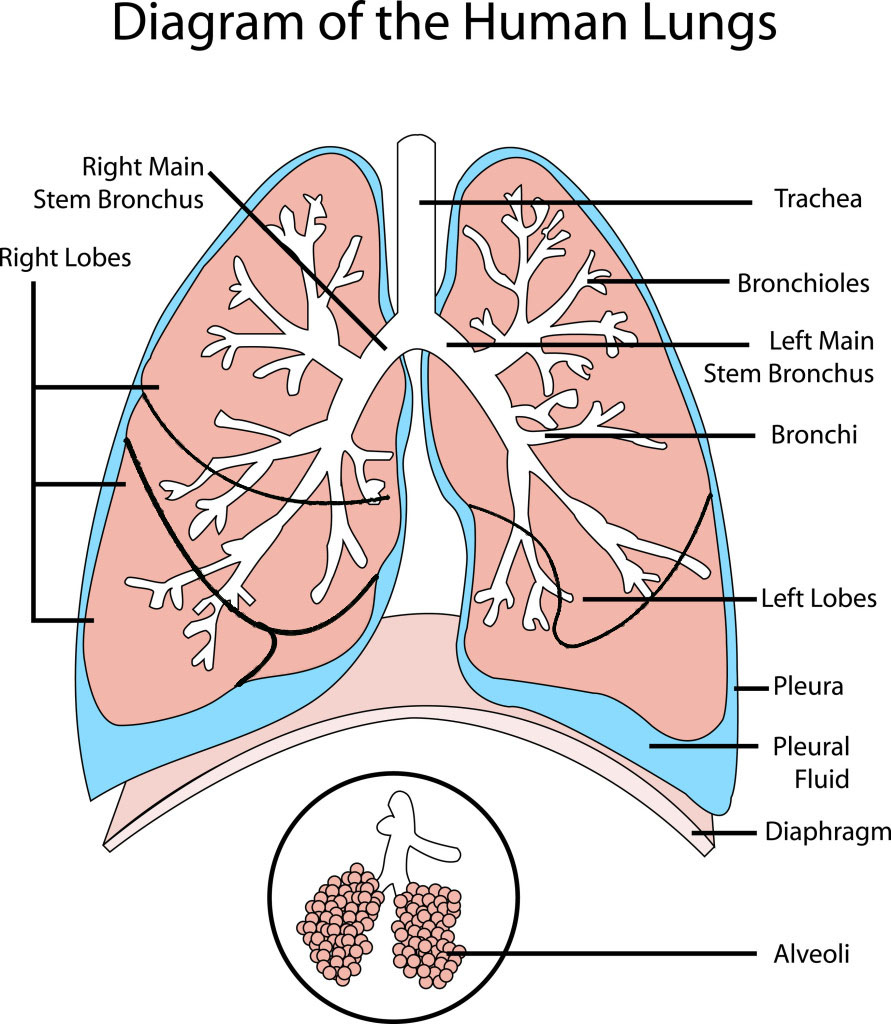
\includegraphics[height=2.7in]{Segmentation/Image/LobeAnatomicalStructure.jpg}
  \caption{Schematic diagram of anatomical lung structure, showing the major airways, lobes and major fissures. The lungs are subdivided into the right upper (RU), right middle (RM), right lower (RL), left upper (LU), and left lower (LL) lobe. The pleural cavity which surrounds the lung consists of a double membrane layer (visceral pleura and parietal pleura) separated by a thin layer of pleural fluid. The inner membrane (visceral pleural) folds inwards between the lobes, creating fissures. Reproduced from \citep{doel2015review}.}
  \label{fig:LobeAnatomicalStructure}
\end{figure*}

%%%%%%%%%%%%%%%%%%%%%
\subsection{High resolution computed tomography}
CT imaging is a typical image modality used in diagnosis and management of IPF. It acquires multiple X-ray images at different orientations and reconstructs these images to obtain tomographic views in the region of interest \citep{zhang2011medical}. This kind of imaging modality is typically used in clinical applications and research regarding pulmonary structure-function relationships \citep{hoffman1997assessment}, including detection of both acute and chronic changes in the lung parenchyma. It is particularly relevant here because normal two-dimensional X-rays can not show subtle  defects. For evaluation of chronic interstitial processes (emphysema, fibrosis, and so forth), thin sections with high spatial frequency reconstructions are used \citep{coxson2007computed}. Scans are often performed both in inspiration and expiration. This special technique is called \gls{hrct}. With the help of \gls{hrct} scans, a series of high-resolution chest sections can be acquired with slice thickness as low as 0.5 mm \citep{naidich2005imaging}, which can provide high visibility of the lung boundaries and pulmonary fissures.  By making use of some advanced image processing technologies, a wide variety of features can be detected from these images such as density of the lung \citep{coxson2007computed}, volumes of the lung \citep{hu2001automatic}, the regions of lung disease distributions \citep{el2013computer, ley2008quantitative}, airway trees \citep{graham2010robust, zhu2010automatic, diaz2010airway} and blood vessels \citep{shikata2009segmentation}. Computed tomography (CT) images acquired at different stages in the breathing cycle can also be used to study lung mechanics and estimate regional lung ventilation \citep{hoffman2006state, yamamoto2011investigation}.

%%%%%%%%%%%%%%%%%%%%
\subsection{The importance of pulmonary lobar segmentation}
The extraction of pulmonary lobes from CT scans is of great importance for lung disease assessment and treatment planning. For clinical applications, the distribution and location of pulmonary disease are beneficial information for doctors to recognize pathogenesis, guide therapy and have further value in surgical planning. That is, because many pulmonary diseases are more prevalent in specific anatomic regions of the lung, often acting at a lobar level. For example, emphysema \citep{jeffery1998structural}, postprimary tuberculosis \citep{leung1999pulmonary} and silicosis \citep{rees2007silica} usually affect the upper lobes, while idiopathic pulmonary fibrosis is commonly present in the lower lobes \citep{lin2015combined}. However, there is currently a lack of quantitative and objective methods for the regional assessment of lung disease. Therefore, it is important to develop techniques that can identify the location, shape and volume of the lobes so that lung disease can be measured at a lobar level and the severity can be assessed accurately.

% Section 2
\subsection{Challenges of automatic pulmonary lobar segmentation from CT scans} \label{SegmentationChallenge}
The most commonly used method to segment lobes from \gls{ct} is through manual assessment by an experienced pulmonary radiologist. However, the process of determining the lobar boundaries is extremely laborious and a time-consuming task, typically taking hours for one patient. This is because a 3D \gls{hrct} image may contain a large number of axial slices which makes the manual segmentation very time consuming. Therefore, doctors rarely use manual lobe segmentation in clinical diagnosis and treatment in practice, and most clinicians use subjective visual observation. For this reason, an automatic (no user interaction) or semi-automatic (minimal user interaction) lobe segmentation technique is urgently needed in clinical applications and this has attracted great interest from researchers all over the world \citep{van2013automated,pu2009computational,ukil2009anatomy}.

However, to find an effective and time-saving automatic lobe segmentation method is a challenging task because of anatomical variation and the possibility of incomplete fissures. Lobar structures vary significantly between subjects, and the anatomical variation in lobe structure is usually associated with age, sex and body type. Pathologies of diseased lungs usually deform the lobar shape abnormally and result in fuzzy appearance of fissures on \gls{ct} images, in particular when abnormalities are present near the fissures, which makes fissure segmentation challenging. Even in patients with healthy lung parenchyma, fissures are sometimes incomplete \citep{gulsun2006variability, doel2015review} (see Figure \ref{fig:FissureSegmentationChanllenges}).

\begin{figure*}[htbp]
  \centering 
  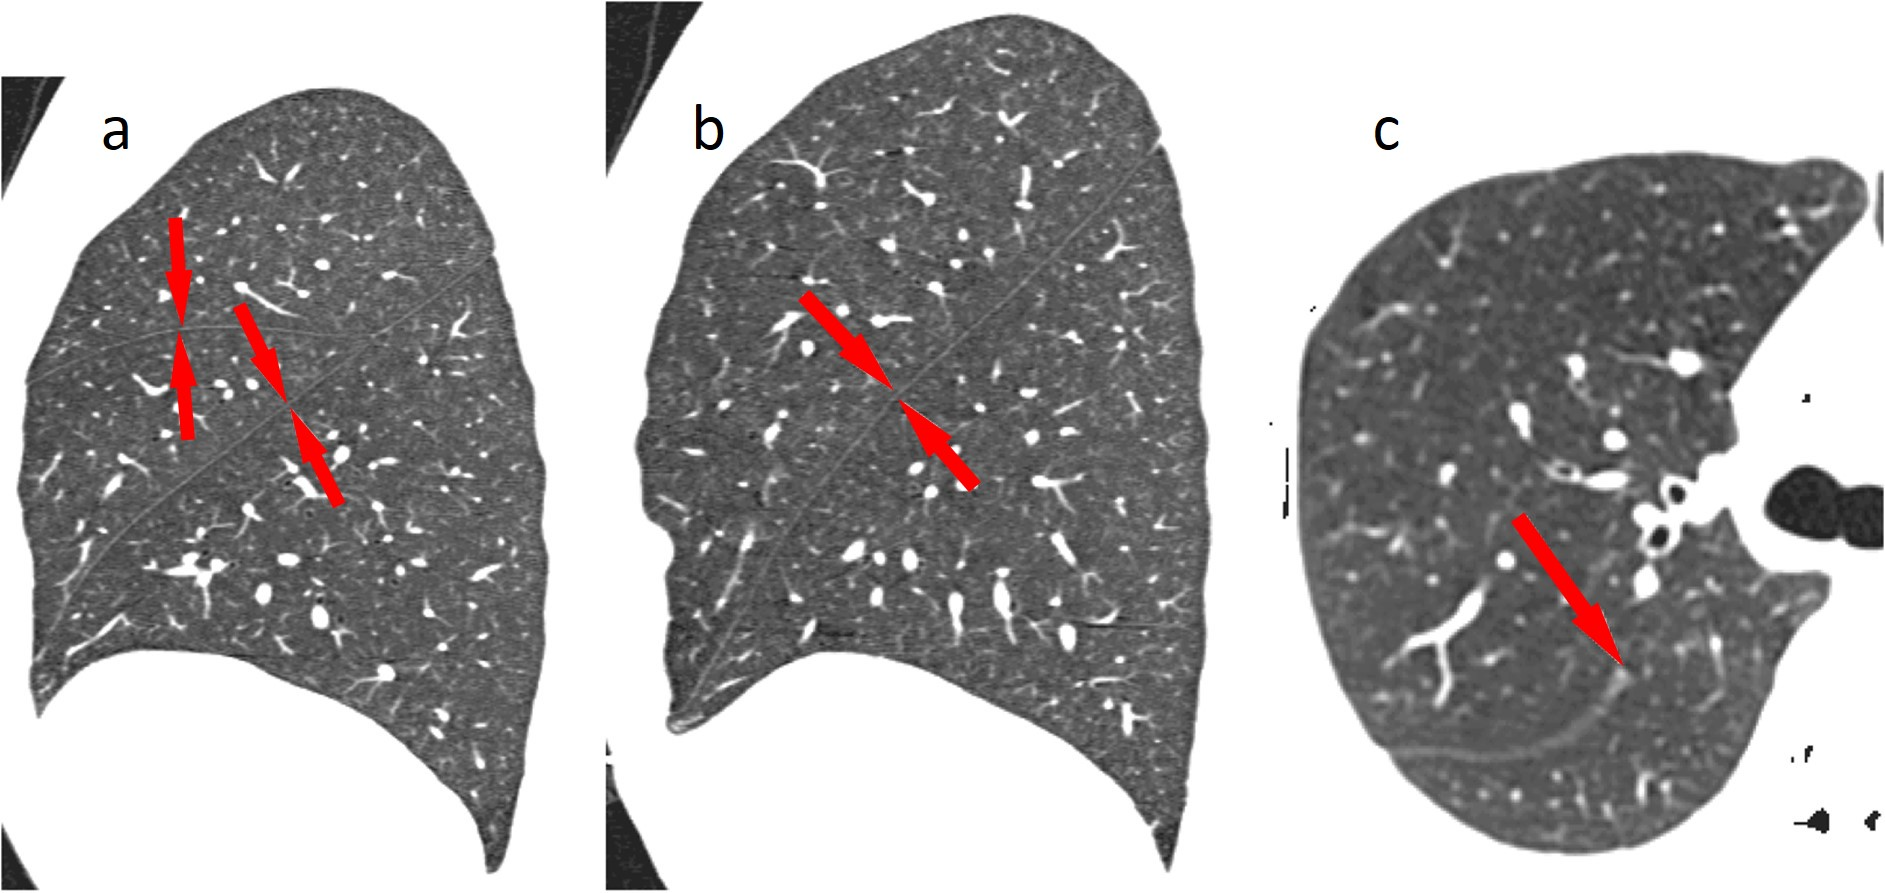
\includegraphics[height=1.75in]{Segmentation/Image/FissureSegmentationChanllenges.jpg}
  \caption{Slices of lung CT images illustrating the left and right fissures. Fissures are visible as white lines of high density tissue crossing the low density lung parenchyma. (a) Sagittal slice from the right lung showing the right oblique and horizontal fissures, the horizontal fissure is oriented horizontally. (b) Sagittal slice from the left lung showing the left oblique fissure. (c) Transverse slice from a different data set that show an incomplete right oblique fissure. Reproduced from \citep{ukil2009anatomy}.}
  \label{fig:FissureSegmentationChanllenges}
\end{figure*}

% Section 3
\section{Review of current published methods for pulmonary lobar segmentation} \label{SegmentationReview}
In a broad sense, existing lobe segmentation methods usually consist of two steps: the segmentation of lungs, and the detection of the three main pulmonary fissures \citep{van2013automated}. Currently, a number of lung segmentation methods are available and most produce reliable results for normal lung at end-inspiration \citep{hu2001automatic,ukil2005smoothing,sun20063d,pu2008adaptive,wang2009automated}. In contrast, most challenges of automated lobar segmentation lie in the fissure detection, and currently no method has yet been demonstrated to be robust and effective across a wide range of clinical imaging parameters and pathology experienced in clinical practice. Lung lobe segmentation is a complex multi-stage process that cannot be addressed by a simple algorithm \citep{van2013automated,pu2009computational,ukil2009anatomy}. However, to some extent, lung segmentation and fissure detection are two independent parts and can be improved separately. That is, it should be possible to change lung segmentation in one way or another without affecting the fissure detection result dramatically. In the following section, existing work is discussed to highlight the key challenges of lobe segmentation algorithms, focusing on these two parts of the process. Then, a new approach to lung and lobe segmentation is presented.

%%%%%%%%%%%%%%%%%%%%%%%%%%%%
\subsection{Lung segmentation}
Segmentation of lung is a prerequisite for the accomplishment of lobe segmentation, as it provides a boundary condition for subsequent fissure detection, allows estimation of lung volumes, and helps to detect and quantify abnormalities within the lungs. While not precisely defined, the lung region is usually considered to be the volume enclosed within the pleura, including the lung parenchyma, airways and vessels, but excluding those parts of the major airways and vessels which extend the pleural boundary. In this section, published methods for lung segmentation are briefly discussed. These methods are summarized in Table \ref{tab:LungSegmentationSummary}.

\newcolumntype{C}[1]{>{\centering\arraybackslash}p{#1}}
\begin{table}[htbp]
\centering
\caption{Summary of lung segmentation methods}
\label{tab:LungSegmentationSummary}
\begin{tabular}{|p{4.3cm}|p{6.3cm}|p{4.8cm}|}
\hline
\bf{Authors} & \bf{Algorithms} & \bf{Notes}\\ 
\hline
\cite{kalender1991semiautomatic,kemerink1998segmentation,leader2003automated} & 2D thresholding method &  1. May cause discontinuity between slices; 2. Time consuming\\
\hline
\cite{keller1981automatic,hedlund1982two,hoffman1983noninvasive,hoffman1985effectb} & Early-stage 3D thresholding method combined with manual interaction & Causes too many intra-operator errors\\
\hline
\cite{hu2001automatic} & 1. Automatically choose thresholding value; 2. Separate left and right lung 3. Morphological lung boundary smoothing & First group to apply fully automatic 3D thresholding method\\
\hline
\cite{ukil2005smoothing} & 1. Bounding box defined around mediastinum; 2. Extract left and right main stem bronchi; 3. 3D Morphological boundary closing & Automatic method using airway tree information\\
\hline
\cite{sun20063d} & 1. Anisotropic filtering; 2. Wavelet transform-based interpolation to construct 3D data; 3. Adaptive 3D region growing combined seed-locating to detect lung region; 4. Fuzzy logic algorithm and 3D morphological to fill hole & 3D method using signal-to-noise ratio\\ 
\hline
\cite{kitasaka2003lung} & 1. Affine transformation to fit a contour shape model to individual images; 2. Active contour model to refine initial segmentations in 3D & Solves the problem of lesions adjacent to the chest wall and mediastinum\\
\hline
\cite{pu2008adaptive} & 1. 3D initial thresholding processing; 2. Adaptive border marching & Minimizes oversegmentation of adjacent regions such as abdomen and mediatinum\\
\hline
\cite{pu2011shape} & 1. Principal curvature analysis to eliminate noise; 2. Radius basis function to smooth lung in 3D & Solves the problems of disease, noise or artifacts\\
\hline
\cite{prasad2008automatic} & 1. 3D thresholding algorithm; 2. Adapt lung curvature using rib curvature; 3. Morphologic operation & 1. Uses rib curvature information to define lung borders; 2. Solves the problem of error detection for lung pathologies\\
\hline
\cite{wang2009automated} & 1. 3D thresholding processing; 2. Texture analysis to identify abnormal regions; 3. 2D hole filling & Texture feature analysis to segment \gls{ild} lungs\\
\hline
\cite{sun2012automated} & 1. Active shape model to roughly find lung outlines; 2. Optimal surface finding to adapt final segmentations & 3D method using rib information\\
\hline
\end{tabular}
\end{table}

\subsubsection{Conventional lung segmentation methods}
In \gls{ct} scans from healthy subjects, the air-filled lung parenchyma usually has a lower attenuation level compared to surrounding high-density tissue at the pleura. For this reason, many conventional lung segmentation algorithms adopt a thresholding approach to search for a large connected region of the air-like values within the image. Threshold values are acquired from grey level histogram analysis and then an initial lung region is detected. A region growing method for the airways is usually applied subsequently to exclude the trachea and major airway branches. Some thresholding algorithms, especially older studies, were developed in 2D space, which means each axial section of \gls{ct} imaging needs to be analysed separately \citep{kalender1991semiautomatic,kemerink1998segmentation,leader2003automated,armato2004automated}. A 2-D method is a logical choice in the case of thick-slice \gls{ct} data, but it may cause discontinuity between slices. Therefore, as higher resolution isotropic data became available, improved 3D processing methods were developed to avoid slice inconsistencies and reduce time for segmentation \citep{hu2001automatic,ukil2005smoothing,sun20063d}.

Most early 3D thresholding-based lung segmentation methods \citep{keller1981automatic,hedlund1982two,hoffman1983noninvasive,hoffman1985effecta,hoffman1985effectb} required significant manual interaction. This interaction included manually selecting threshold values or seed points for region growing, and separating left and right lungs manually. This leads to a process that is consuming and is subject to intra-operator errors. \cite{hu2001automatic} was the first group to apply a threshold-based algorithm in a fully automatic lung segmentation method. In their study, the lung region was firstly extracted from the CT images by gray-level thresholding processing. Instead of a fixed threshold value, an optimal thresholding method was used to automatically choose a threshold value that reflects the grey-scale characteristics of a specific dataset. The left and right lungs were then separated by identifying the anterior and posterior junctions by dynamic programming. Finally, a sequence of morphological operations was used to smooth the irregular boundary along the mediastinum.

\cite{ukil2005smoothing} developed an improved automatic lung segmentation method to smooth lung boundaries in 3D using information from the segmented airway trees. A bounding box was first defined around the mediastinum for each lung using information from the segmented human airway trees, and all operations were then performed within the bounding box. After that, all generations of the airway distal branches were defined to the left and right main stem bronchi to be part of the respective lungs, and all the other segmented structures could be excluded. Finally, a fast morphological closing with an ellipsoidal kernel was performed to smooth the surface of the lung. This method solved the problem of irregular and inconsistent lung boundary of the regions near the mediastinum by using a common threshold algorithm. 

\cite{sun20063d} presented a 3D-based method for segmenting lungs with improved accuracy. An anisotropic filtering method was first applied on \gls{ct} slices to enhance the signal-to-noise ratio. A wavelet transform-based interpolation method was subsequently used to construct the 3D volumetric \gls{ct} slice data with volume rendering. After that, an adaptive 3D region-growing algorithm was developed to detect the lung region, combined with automatic seed-locating methods. Fuzzy logic algorithms and 3D morphological closing approaches were finally used to refine the lung volume and fill the holes in it. The method was effective and, in general, robust with an average accuracy rate of 88.5\%.  

\subsubsection{Specially designed lung segmentation methods for abnormal lungs}
Although conventional threshold-based methods are fast, robust and typically accurate for healthy subjects, they may fail to perform well for scans containing physiologic abnormalities, which often results in segmentation errors and requires manual editing of the results (see in Figure \ref{fig:AbnormalLungSegmentation}). Currently, specially designed lung segmentation methods mostly focus on a single lung disease and therefore can not get a good result across a large population \citep{kitasaka2003lung,sluimer2005toward,pu2008adaptive,pu2011shape,prasad2008automatic,korfiatis2008texture,wang2009automated,van2009automatic,sun2012automated}. 

\begin{figure*}[htbp]
  \centering 
  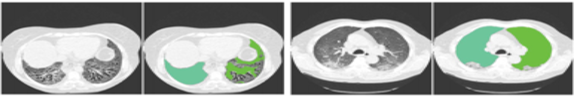
\includegraphics[height=1.5in]{Segmentation/Image/AbnormalLungSegmentation.png}
  \caption{Illustration of the performance of conventional 3D thresholding lung segmentation methods on pathological lungs. Lung borders are not recognized accurately because of the higher densities of the abnormalities compared to the normal tissues. Reproduced from \citep{van2013automated}.}
  \label{fig:AbnormalLungSegmentation}
\end{figure*}

To deal with the problem of lesions adjacent to the chest wall and mediastinum, \citep{kitasaka2003lung} developed a lung area extraction method using a shape model. A contour shape model using a B\'ezier surface was fitted to the contour surface of the individual input images with an affine transformation method. Then, an active contour model was utilized to refine the initial segmentation. The results showed that most lesions could be identified accurately using this method. However, as the lung apex and base were not included in the model, lesions adjacent to the lung apex or diaphragm could result in segmentation errors.

\cite{pu2008adaptive} presented a lung segmentation algorithm based on adaptive border marching (ABM) to include juxtapleural nodules in the lung region since these nodules may be excluded from the results calculated by a conventional threashold-based algorithm. The adaptive border marching algorithm could smooth the lung borders after an initial thresholding processing and minimize over-segmentation of adjacent regions such as the abdomen and mediastinum. The method was tested on 20 datasets and the results demonstrated that this method could re-include all juxtapleural nodules in the lung regions. An average over-segmentation ratio of this method was 0.43\% which was lower than the reference standard average segmentation determined by an expert. In order to deal with the problem of different types of lung disease, image noise or artefacts, and individual anatomical variety, \cite{pu2011shape} developed a shape analysis strategy termed ''break-and-repair''. A principal curvature analysis was applied to eliminate the problematic regions and then radial basis function (RBF) based implicit surface fitting was used to get a smooth lung surface. 

To overcome the error in detection of the lung boundaries for lung pathologies, \cite{prasad2008automatic} made use of rib curvature information to help with finding the lung borders. The method was based on a threshold-based algorithm followed by a morphologic operation. The core principle of the method was to adapt the threshold value to an individual subject by making the curvature of lung along the ribs be similar to the curvature of the ribs. These curvatures were both represented by polynomial interpolation even though there was minimal deviation from this representation. The results showed that the performance of the rib segmentation method was better than the same method without guidance from rib segmentation.

\cite{wang2009automated} proposed a texture analysis-based method to segment ILD lungs. The lung region including normal and mild ILD lung parenchyma was first segmented by a CT value thresholding technique and then texture-feature images derived from the co-occurrence matrix was used to identify abnormal lung regions with severe ILD from the initial results. 2D hole filling was applied to smooth the final lung segmentation. The overlap rate, volume agreement, mean absolute distance (MAD), and maximum absolute distance between the automatically segmented lungs and the reference lungs (delineated manually by a medical physicist) were employed to evaluate the performance of the segmentation method, and showed accurate lung segmentation results for abnormal CT scans with severe ILD.

On the basis of the previous studies, \citep{sun2012automated} developed a further approach for segmentation of lungs with high-density pathologies. The method had two main steps. In the first step, a robust active shape model (RASM) matching method was utilized to roughly find the outline of the lungs. To initialize the shape model of RASM, detected rib information was used. In the second step, an optimal surface finding approach was applied to further adapt the initial segmentation result to the lung. The method was evaluated on both normal and abnormal subjects and had a better performance compared to two commercially available lung segmentation approaches.
%%%%%%%%%%%%%%%%%%%%%%%%%%%%%%%%%%%
\subsection{Fissure detection}
The currently published fissure detection methods can be, for the most part, classified into two categories: anatomical knowledge based analysis methods and shape based analysis methods. Anatomical knowledge based methods usually depend on either local or global knowledge of the anatomy of lung structure based on two pulmonary anatomical features. The first feature is the fact that there should not be any large vessels in the vicinity of lobar fissures, so fissures should locate in the gaps between airway and vessel trees. Another feature is that the airway bronchi can be classified into five lobar branches using an edge detection method (Figure \ref{fig:AnatomicalBasedSegmentation}). Shape based analysis methods commonly make use of gray-level information and shape information to detect the fissures. Published fissure detection methods are summarized in Table \ref{tab:FissureDetectionSummary}.

\begin{figure}[htbp] 
\centering
\begin{subfigure}{.3\linewidth}% set image scale
  \sbox0{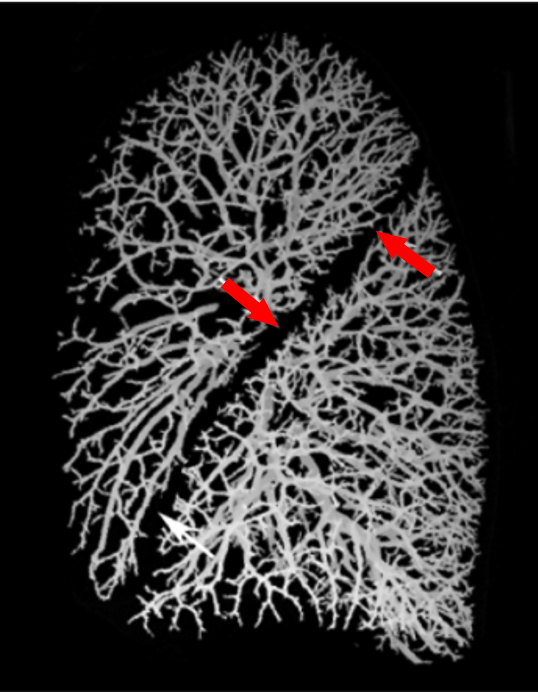
\includegraphics{Segmentation/Image/VolumetricVesselTree.png}}
  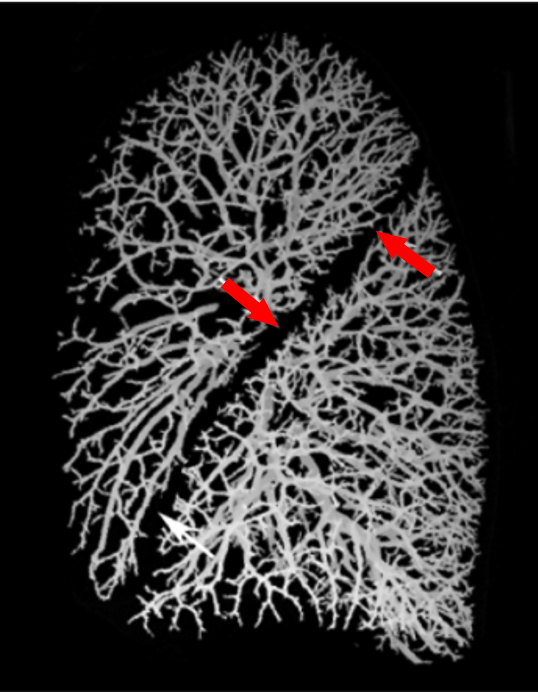
\includegraphics[width=\linewidth,trim={{.0\wd0} {.0\wd0} {.0\wd0} {.0\wd0}},clip]{Segmentation/Image/VolumetricVesselTree.png}
  \caption{}
  \label{fig:AnatomicalBasedSegmentation-a} 
\end{subfigure}
%\vspace{.3in} % control space between the upper context and figure
\hspace{.6in} % control space between two figures
\begin{subfigure}{.43\linewidth}% set image scale
  \sbox0{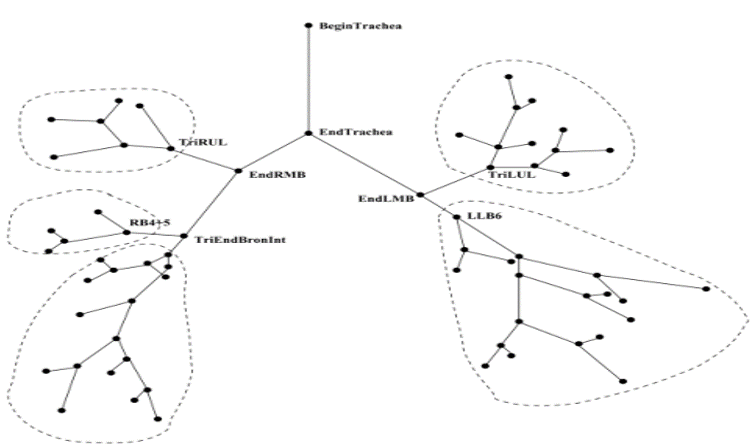
\includegraphics{Segmentation/Image/LabelledAirwayTree.png}}
  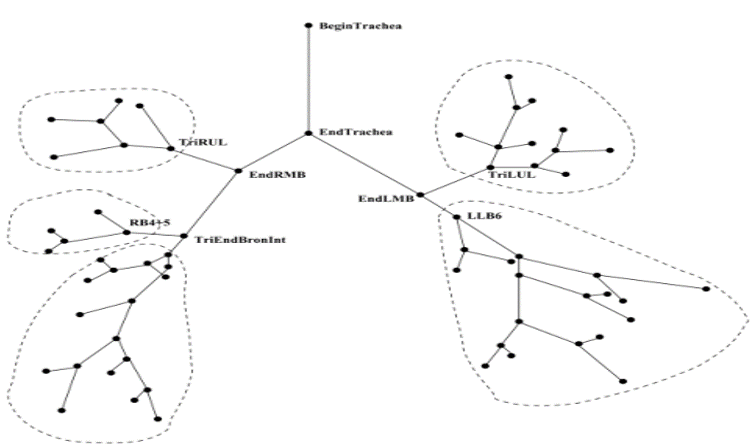
\includegraphics[width=\linewidth,trim={{.0\wd0} {.0\wd0} {.0\wd0} {.0\wd0}},clip]{Segmentation/Image/LabelledAirwayTree.png}
  \caption{}
  \label{fig:AnatomicalBasedSegmentation-b} 
\end{subfigure}
\caption{(a) Segmented volumes of the vascular tree. There are no large vessels in the vicinity of lobar fissures. (b) Anatomically labeled airway tree showing lobar subtrees. The airway tree can be classified corresponding to five lobes. Reproduced from \citep{ukil2009anatomy}.}
\label{fig:AnatomicalBasedSegmentation}
\end{figure}

\newcolumntype{C}[1]{>{\centering\arraybackslash}p{#1}}
\begin{table}[htbp]
\centering
\caption{Summary of fissure detection methods}
\label{tab:FissureDetectionSummary}
\begin{threeparttable}
\begin{tabular}{|p{4.3cm}|p{6.3cm}|p{4.8cm}|}
\hline
\bf{Authors} & \bf{Algorithms} & \bf{Notes}\\ 
\hline
\cite{kuhnigk2003lung,kuhnigk2005informatics} & Watershed transformation method to analyze anatomical structures to help with fissure detection &  First group to use lobar airways and vasulature into fissure detection\tnote{1}\\
\hline
\cite{ukil2009anatomy} & 1. Watershed transform guided cost image to define initial fissures; 2. Construct ROI; 3. Structure tensor analysis combined with optimal surface detection to find fissure surface; 4. Fast marching method to detect incomplete fissures & 1. Improved on Kuhnigsk's method; 2. Can detect incomplete fissures\tnote{1}\\
\hline
\cite{lassen2010automatic} & Watershed transformed anatomical structure based method & An extension of Kuhgigk's method\tnote{1}\\
\hline
\cite{zhou2004automatic,saita2006algorithm} & 1. Edge detection to class vessels and bronchi; 2. Hough transform to detect curve surface & Take advantage of linear appearance of fissures\tnote{1}\\
\hline
\cite{wang2004shape,wang2006pulmonary} & 1. Identify initial fissure ROI; 2. ''Ridge map'' based tranformation to enhance initial fissure; 3.  Shape-based curve growing to get the finial fissures. & 2D shape based method\tnote{2}\\
\hline
\cite{frangi1998multiscale} & Hessian matrix based analysis to extract local image structures & The first paper to apply Hessian matrix analysis on image segmentation in 3D\tnote{2}\\
\hline
\cite{wiemker2005unsupervised} & Combine first derivative and second derivative of image gray values to find fissures & An early paper using Hessian matrix on fissure detection\tnote{2}\\
\hline
\cite{ochs2007automated,van2008supervised} & Use pattern recognition approach and Hessian matrix and classification operation to detection fissure & An improved Hessian based method\tnote{2}\\
\hline
\cite{lassen2011interactive,lassen2013automatic} & 1. Use anatomical structures to acquire initial fissue; 2. Hessian matrix surrounding initial guessing areas; 3. Morphological operations to filter noise & Combine both anatomical information and gray-level information\tnote{1,2}\\
\hline
\cite{doel2012pulmonary} & 1. Use both anatomy knowledge and Hessian matrix to find fissure candidate points; 2. Multi-level B-spline curve to get the finial fissure surface. & Combine both anatomical information and gray-level information\tnote{1,2}\\
\hline
\cite{ross2010automatic,ross2013pulmonary} & 1. Particle system combined with Hessian matrix to get candidate fissure points; 2. Maximum a posterior method to remove noise points; 3. Thin plate spline to form finial fissure surface. & Effective for lung lobe segmentation in absence of complete anatomical structures on CT imaging\tnote{2}\\
\hline
\end{tabular}
\begin{tablenotes}
        \footnotesize
        \item[1] Anatomy knowledge based method.
        \item[2] Shape based analysis method.
\end{tablenotes}
\end{threeparttable}
\end{table}

\subsubsection{Anatomical knowledge based method}
Methods that aim to detect the lobar fissures usually start by finding an approximate location of the lobar borders based on prior anatomical knowledge of lung structures in order to narrow the search area for fissure detection \citep{kuhnigk2003lung,kuhnigk2005informatics,zhou2004automatic,saita2006algorithm,zhang2006atlas,ukil2009anatomy,pu2009computational,lassen2010automatic,doel2012pulmonary}. These methods are developed mainly based on two pulmonary anatomical features. A number of published papers use the segmentation results of airways and vessels to help localize fissures. Usually, the vascular segmentation provides more accurate estimation of lobar fissure locations than the airway trees, since more vessel generations can be detected from \gls{ct} scans. These vessels span the entire lung volume which can help to find complete gaps between lobes. However, airways also play an important part in initial estimation of fissures, since airways trees can be more reasonably divided into lobes based on branching structure, while the structure of vasculature branching is more complicated to extract from images and some connections are hard to separate accurately. Therefore, a lot of studies make use of both vessel and airway information to guide fissure detection \citep{ukil2009anatomy,lassen2010automatic,doel2012pulmonary}.

\cite{kuhnigk2003lung,kuhnigk2005informatics} was an early group to present a framework of taking both lobar airways and vasculature into account for automatic fissure detection. A watershed transformation method has been used to take an analysis of these anatomical structures and this method was widely used and improved by other researchers, but the results calculated by this simple algorithm were not accurate enough even for some clearly visible fissures. 

\cite{ukil2009anatomy} developed Khnigk's fissure detection method which used a distance transform to combine segmented vessels, lobar airways, and original chest CT scan as a cost image to guide initial fissure guessing. They found that the improved watershed transform algorithm could provide a close initial approximation to the lobar fissures. Subsequently, a refinement method was used to construct a region of interest (ROI) which encompasses the fissures. A 3D optimal surface detection algorithm combined with a 'ridgeness' measurement was then applied to enhance the ROI, and find the optimal surface within the ROI. Finally, incomplete fissures were smoothly extrapolated using a fast-marching method based segmentation of a projection of the optimal surface. This method is able to segment incomplete fissures, and so significantly improved on prior methods.

\cite{lassen2010automatic} also described a fissure detection method by building a cost image for the watershed transformed segmentation which is an extension of the framework of Kuhnigk. The interactive segmentation method was tested on 25 \gls{ct} scans comparing to a manual segmentation by a human observer and showed an average error distance of 1.57$ \pm $0.3mm. In addition, \cite{zhou2004automatic} and \cite{saita2006algorithm} took advantage of the linear appearance of fissures to class the vessels and bronchi into five lobe regions using an edge detection method and used a Hough transform based curved surface detection method. 

\subsubsection{Shape based analysis method}
Generally, lobar fissures can be regarded as bright planes crossing the pulmonary volume because of the higher density value of fissures compared to the surrounding tissues. Based on this information, quite a number of published methods use a local filtering algorithm to detect the voxels which lie on these planes, so that these detected voxel points can construct a continuous fissure surface. In 2D space, the fissure appears as a clear curve, therefore some early papers usually detected fissure points based on gray-level information in 2D space. For example, \cite{wang2004shape,wang2006pulmonary} presented a 2D fissure detection method based on shape information. In this paper, the fissure was initially denoted as a curve based on the prior knowledge of the fissure shape to identify the surrounding region of fissure, called ''fissure region'' for subsequent automatic segmentation. Next an image transformation called ''ridge map'' was proposed for enhancing the appearance of initial fissures. A shape-based curve-growing method modeled by a Bayesian network could then be applied to this ''map'' to segment the fissure.

In 3D space, the most commonly used method to detect these pulmonary fissure plane structures is taking an eigenvalue analysis of the Hessian matrix \citep{frangi1998multiscale,wiemker2005unsupervised,kitasaka2006recognition,ochs2007automated,van2008supervised,lassen2011interactive,lassen2013automatic,ross2010automatic,doel2012pulmonary}. \cite{frangi1998multiscale} was the first to present an eigenvalue analysis of the Hessian matrix to detect planar structures (fissures) and tube structures (vessels) on \gls{ct} images. The relationship between three eigenvalues of the Hessian matrix describes the local image structure and so can be used to determine a fissure probability. \cite{wiemker2005unsupervised} also used the Hessian matrix for fissure detection, proposing two 3D filter approaches in this paper. The first filter was based on the first derivatives of the image grey values and utilized the eigenvalues of the local structure tensor. The second filter was based on the second derivatives and utilized the eigenvalues of the local Hessian matrix. 

\cite{ochs2007automated} and \cite{van2008supervised} used a pattern recognition approach to detect pulmonary fissures combined with eigenvalue analysis of the Hessian matrix as feature and classification was also performed on these fissures. \cite{lassen2011interactive,lassen2013automatic} combined both anatomical based and shape based methods which successfully eliminated most false points (points identified as fissure but were not). The first anatomic-based method defined a region of interest, and then the Hessian matrix analysis was used only in this region of interest. The region of interest provides an initial guess for fissure locations. Subsequently, morphological operations such as direction-based connected component analysis were used to further reduce non-fissure points that are incorrectly identified as fissures. \cite{doel2012pulmonary} also made use of both an anatomical knowledge based method and the Hessian matrix to find fissure candidate points and constructed a multi-level B-spline smooth curve through the fissure points and extrapolated this curve to the lung borders to get complete fissure surfaces.

\cite{ross2010automatic, ross2013pulmonary} proposed a particle system that sampled the image domain combined with the Hessian matrix to get a set of candidate fissure locations. A maximum a posteriori (MAP) estimation was then used to eliminate false candidate points, and a post-processing operation was applied to remove remaining noise. A thin plate spline (TPS) interpolating surface fitting method was lastly performed to form the final fissure surfaces. This method is effective for lung lobe segmentation in the absence of complete anatomical structures on CT imaging.

%%%%%%%%%%%%%%%%%%%%%%%%%%%%%%%%%%%%%%%%%%%%%%5
% Section 4
\section{Methods: automatic statistical shape model based lobar segmentation method} \label{SegmentationMethod}
Here, an \gls{ssm} guided method is presented to segment pulmonary lobes from \gls{ct} images. A three-step approach is followed for the lobe segmentation (shown in Figure \ref{fig:WholeWorkflow}): in the first step, a threshold-based lung segmentation method defines the lung boundary; in the second step, an \gls{ssm} is deformed to provide a ''search region'' for fissure locations; in the third step, fissures are located using a Hessian matrix protocol combined with connected component filters and a surface fitting algorithm. The new procedure does not depend on prior segmentation of anatomical structures (airway lobar classification) other than lung shape. A user-interactive interface was also developed for the user to control and visualize the whole segmentation process and to allow do some manual correction on the segmented results, if required.
\newpage

\begin{figure}[H]
  \centering 
  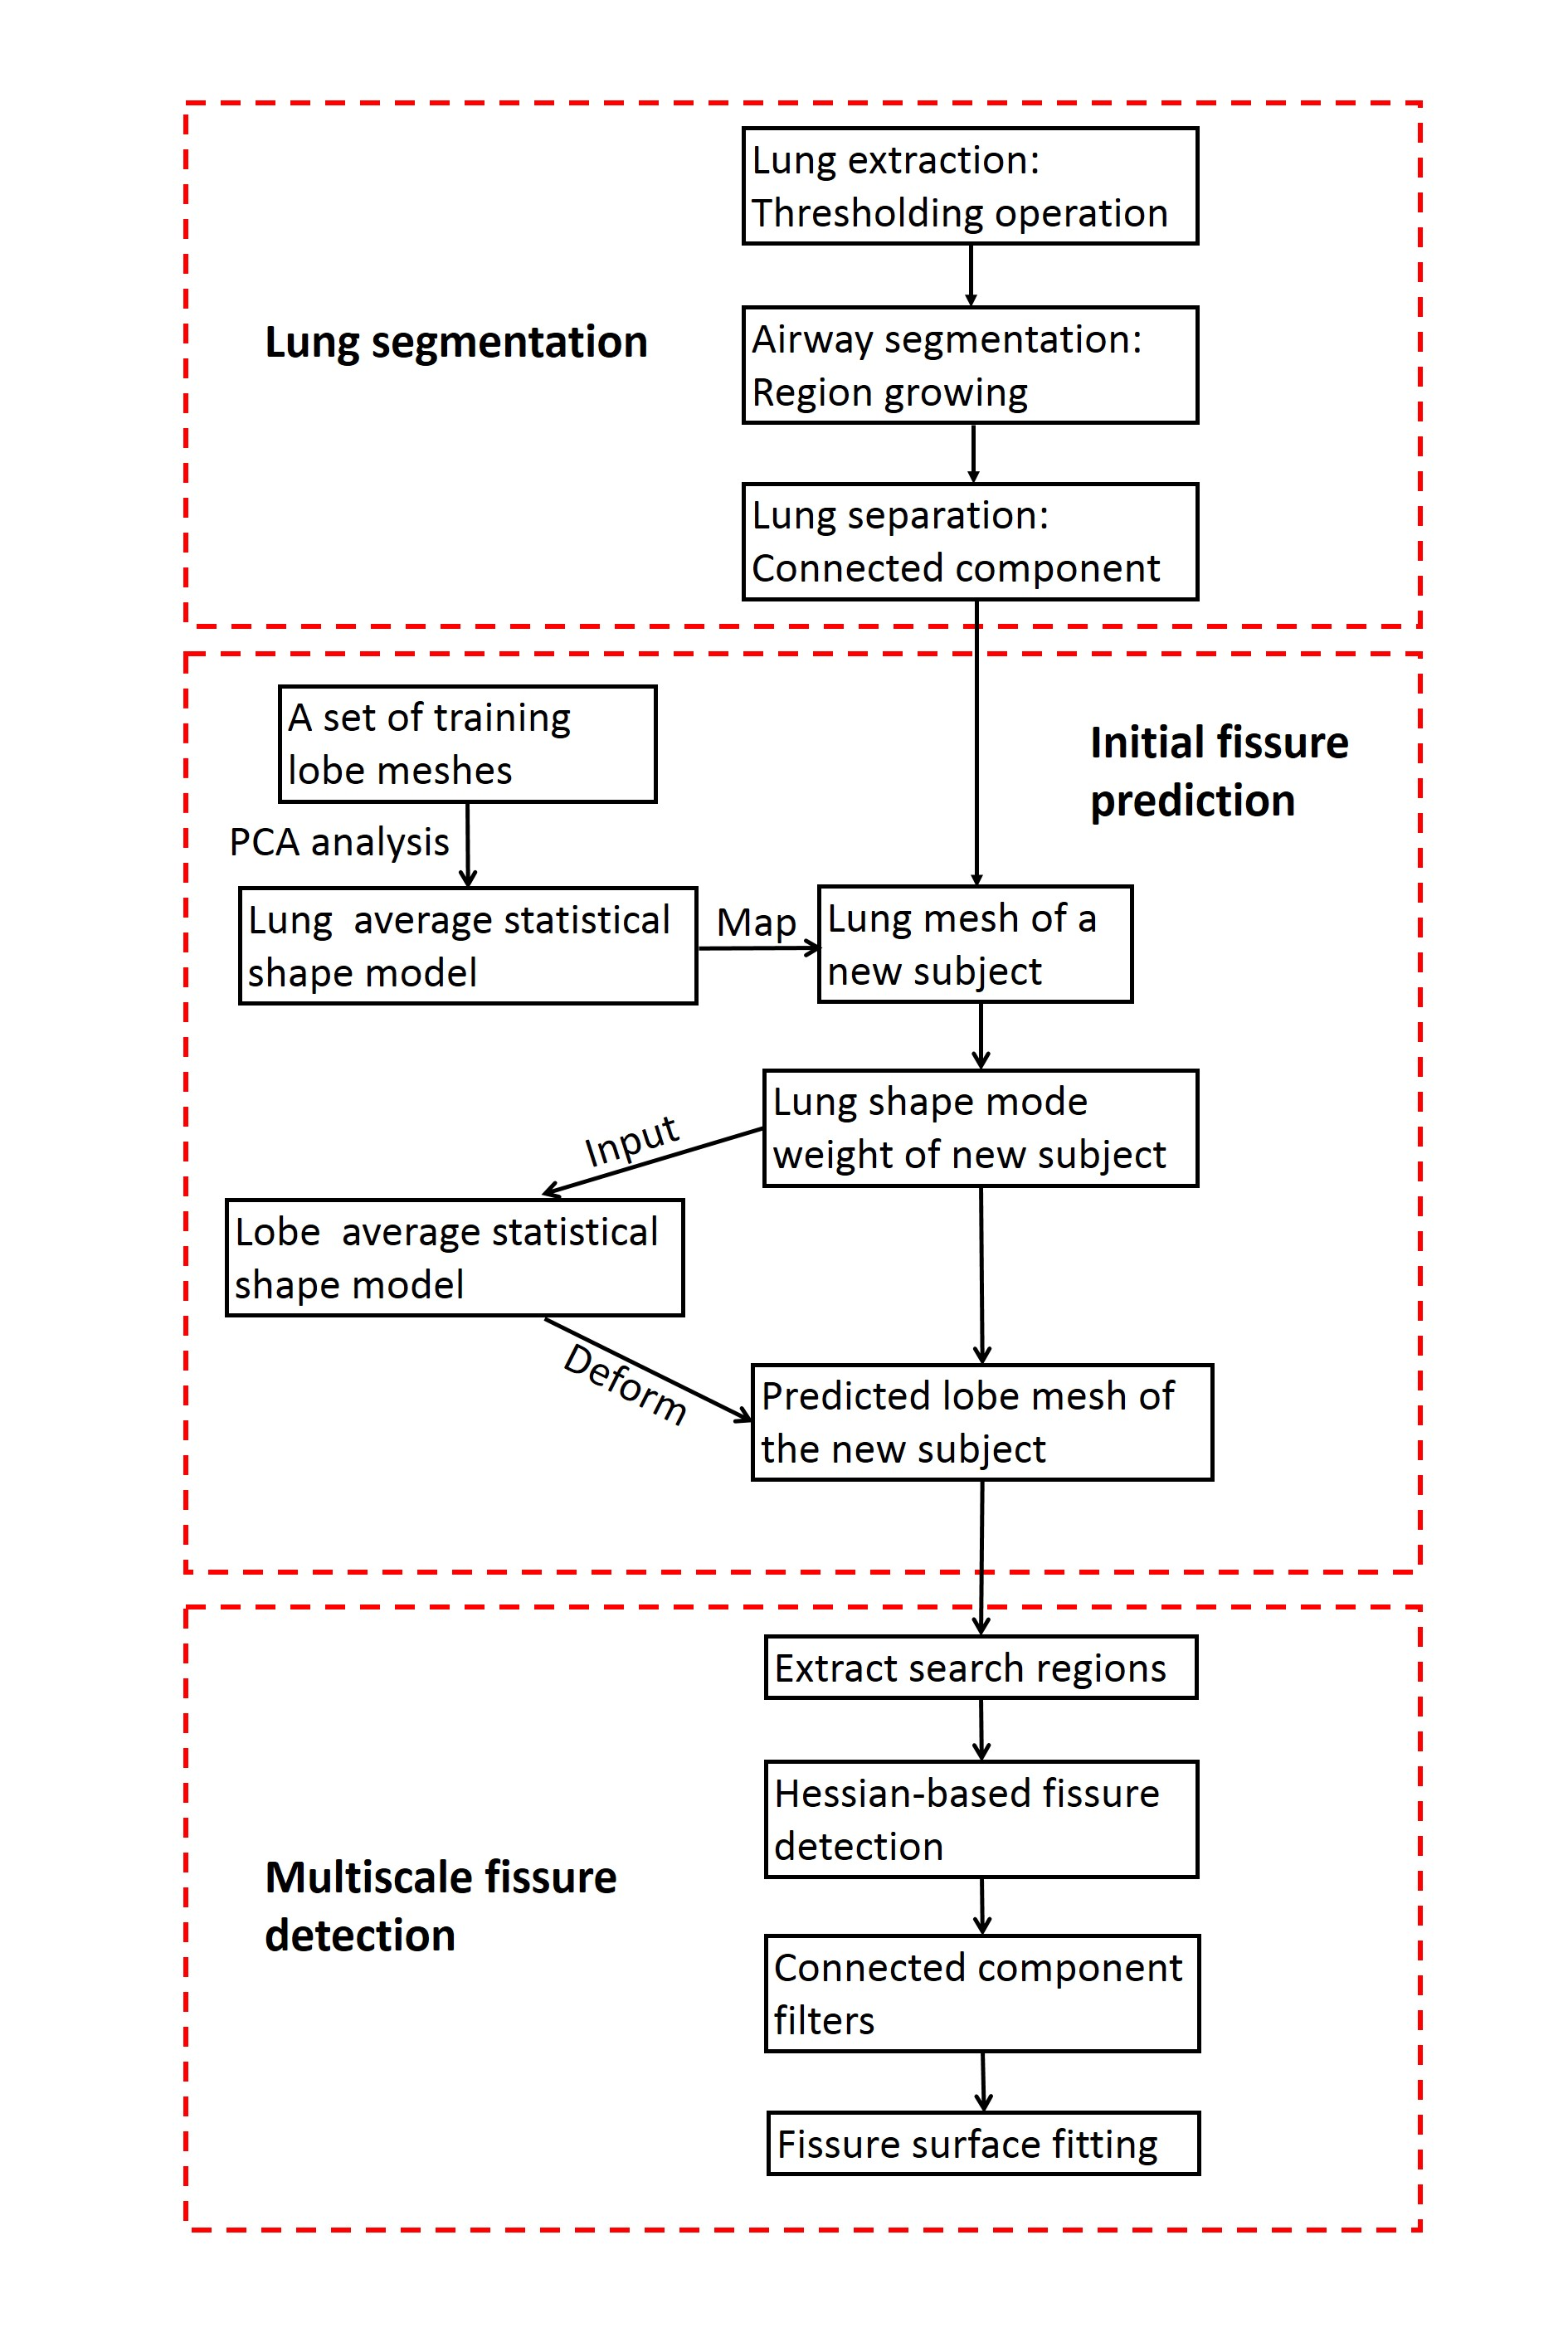
\includegraphics[height=7.8in]{Segmentation/Image/WholeWorkflow.jpg}
  \caption{Flow diagram of the lobar segmentation process.}
  \label{fig:WholeWorkflow}
\end{figure}

%%%%%%%%%%%%%%%%%%%%%%%%%%%%%%%
\subsection{Lung segmentation} \label{subsection:LungSegmentation}
A good lung segmentation is a prerequisite for lobe segmentation, since all the other segmentations need to be performed inside the two lung regions. Here, a common thresholding method was used to segment the lungs \citep{ukil2005smoothing}. The procedure consists of the following steps: 1) uses a thresholding operation (-775 Hounsfield Units) and connected component identification to find the initial lung regions and trachea location, 2) by using the most apical point of the trachea as a starting point, a region growing technique is applied to detect the airway trees, and 3) left and right lungs are separated as the two largest connected components remaining after removing the trachea and main left and right bronchi. Figure \ref{fig:LungSegmentation} shows a typical lung segmentation result.

\begin{figure}[htbp] 
\centering
\begin{subfigure}{.4\linewidth}% set image scale
  \sbox0{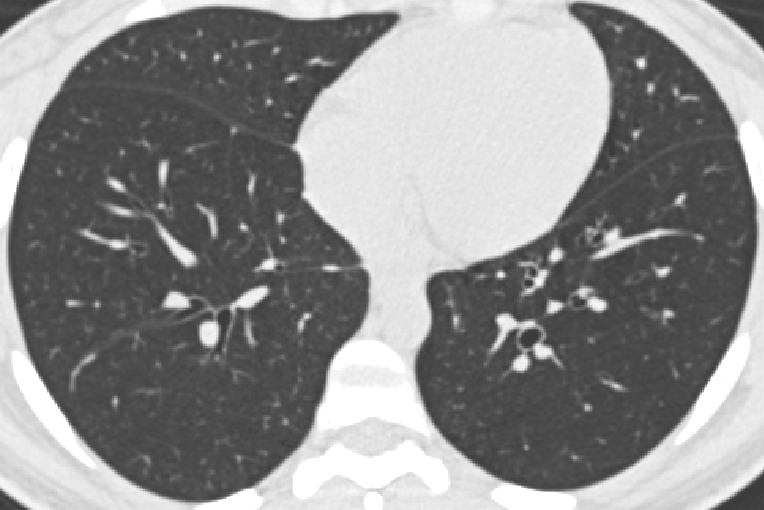
\includegraphics{Segmentation/Image/LungSegmentationBefore.png}}
  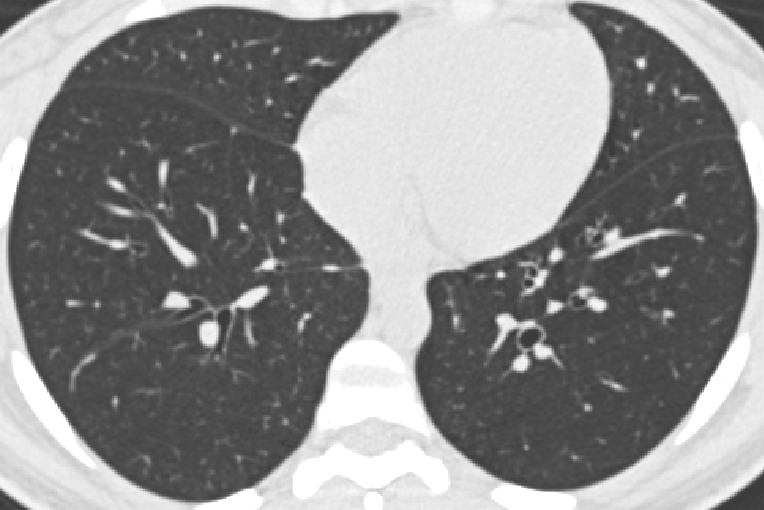
\includegraphics[width=\linewidth,trim={{.0\wd0} {.0\wd0} {.0\wd0} {.0\wd0}},clip]{Segmentation/Image/LungSegmentationBefore.png}
  \caption{}
  \label{fig:LungSegmentation-a} 
\end{subfigure}
\begin{subfigure}{.4\linewidth}% set image scale
  \sbox0{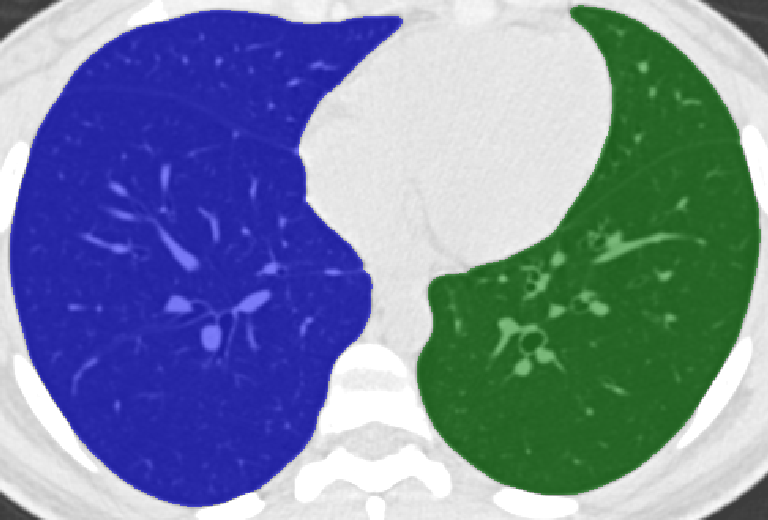
\includegraphics{Segmentation/Image/LungSegmentationAfter.png}}
  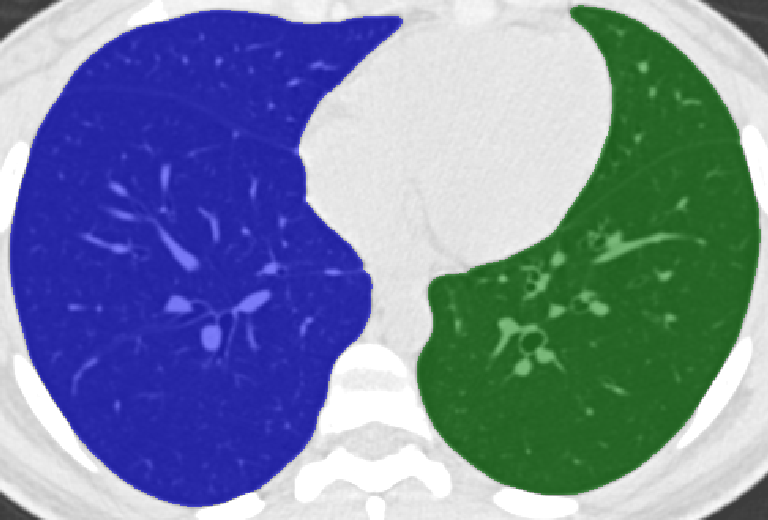
\includegraphics[width=\linewidth,trim={{.0\wd0} {.0\wd0} {.0\wd0} {.0\wd0}},clip]{Segmentation/Image/LungSegmentationAfter.png}
  \caption{}
  \label{fig:LungSegmentation-b} 
\end{subfigure}
\caption{Lung segmentation result using the common thresholding method. (a) Raw CT image. (b) Segmented lungs.}
\label{fig:LungSegmentation}
\end{figure}

%%%%%%%%%%%%%%%%%%%%%%%%%%%%%%%%%
\subsection{Statistical finite element models of lung and fissure shape} \label{ShapeModelGeneration}
For human organs, there is a significant difference in shape and anatomy between different groups of people, such as young and old, male and female, healthy and diseased \citep{krumpe1985aging, crapo1993aging}. This difference is caused by different functional signals and behaviours, leading to organ shape variation across populations. Shape analysis provides a way to understand the underlying mechanisms of those variations in anatomical and physiological processes. The importance of statistical shape analysis in many kinds of biological studies has been well established \citep{dryden1998statistical,stegmann2002brief,styner2003statistical,heimann2009statistical}, because of its potential to capture morphological variation within and between healthy and pathological structures.

Computational model-based approaches to solve problems in image segmentation have become increasingly popular in the last two decades \citep{taylor1995medical,kelemen1999elastic,tsai2003shape,okada2008automated}. In these approaches, each new image set was matched to its expected shape of organ for that individual as a guide for segmentation. This potentially reduces the impact of image artefacts and other perturbations associated with traditional low-level algorithms \citep{ecabert2008automatic,zhang2013development}. To account for individual variations in lung shape and location of fissures (including how they vary with lung inflation), one can analyse a series of training shapes using statistical techniques, leading to a statistical shape model. Using this statistical definition of a cohort of individuals, one can begin to predict an individual's organ shape based on characteristics of that individual to help guide segmentation procedures.

%%%%%%%%%%%%%%%%%%%%%%%%%%%%%%%%%
\subsubsection{Finite element lobar shape modeling} 

To guide a statistical shape model based segmentation, the first step is to generate a statistical lobar shape mesh using a set of training data. Here, we employ a \gls{sfeal} based on an active shape model (ASM) \citep{cootes1995active}. To do this, a training set of segmented lung and fissure surface locations was used to describe a cohort of adults with radiologically normal lungs. This approach employs a finite element shape mesh to specify pulmonary lobar shape which provides an efficient parameterized representation of lobar boundaries and makes shape constraints available during image analysis. The training set consisted of data from 50 subjects. 35 subjects were selected from a study of healthy subjects aged 50 to 100 years, the \gls{aging} study and a further 15 subjects were selected from a separate study of younger healthy subjects, the \gls{hla}. All the \gls{aging} and \gls{hla} subjects are healthy non-smoking subjects including both males and females. In the \gls{aging} group, \gls{hrct} imaging was acquired at Auckland City Hospital using a Phillips Brilliance 16 scanner, with between 400-700 slices per volumetric image. The study was approved by the Northern A Health and \gls{hdec}, Ministry of Health on 29 April 2013 through the \gls{hdec}-Full Review Pathway - ethics reference 13/NT/41. The \gls{hrct} images from \gls{hla} cohort were obtained at the \gls{iclic} using a Siemens Sensation 64 MDCT scanner, with between 500-700 slices per volumetric image. The study was approved by the University of Iowa Institutional Review Board. A summarized population demographics of the subjects used for statistical shape model construction is listed in Table \ref{tab:SSMSubjects}

\begin{table}[htbp]
\centering
\caption{Summarized demographics for the AGING and HLA datasets.}
\label{tab:SSMSubjects}
\begin{tabular}{l c c}
\hline
  & AGING (N=35) & HLA (N=15)\\ 
\hline
Age (years) & 72.3$ \pm $11.41 &  22$ \pm $1.9\\
Sex(M/F) & 18/17 & 5/10\\
Height(m) & 1.66$ \pm $0.14 &	1.7$ \pm $0.1\\
Weight(kg) & 70.6$ \pm $11.1 &	67.6$ \pm $12.2\\
BMI(kg/$\mathrm{m^{2}}$) & 25.6$ \pm $3.0 &	23.3$ \pm $2.2\\
\hline
Ethnicity\\
- Caucasian & 25 &	14\\
- M$\mathrm{\bar{a}}$ori(AGING only) & 1 &	N/A\\
- Asian & 2 &	-\\
- African-American & - &	1\\
 - Unknown & 7 &	-\\
\hline
\end{tabular}
\end{table}

To define the lung shape, volumetric \gls{ct} images were segmented using the method described in Section \ref{subsection:LungSegmentation}. The segmented lung surface was then digitized into a set of data points as a 3D-space representation of lung shape (Figure \ref{fig:LobeShapeGenereation-a}). Fissure surface segmentation was performed manually using the open-source visualization software CMGUI (https://www.cmiss.org/cmgui) by an expert user, to provide a gold-standard definition of the fissure location for each subject in the training set (Figure \ref{fig:LobeShapeGenereation-b}, \ref{fig:LobeShapeGenereation-c}). A high order (bi-cubic Hermite) finite element template mesh with the same mesh connectivity for each subject was geometry fitted to the lung and fissure surface data for each subject. The current lung lobe mesh consists of two separate meshes which represent the left and right lung enclosing the lung parenchymal tissue volume. 

An initial template mesh was created by selecting some data points to be nodes, and then creating two-dimensional surface elements by joining these node points appropriately. The template mesh for the left lung mesh has 35 nodes and 44 elements which described the left lung surface and left oblique fissure, while the right lung mesh has 50 nodes and 62 elements which defined right lung surface, right oblique fissure and right surface fissure. For fitting to lung and lobe shape data, the template mesh was modelled using bi-cubic Hermite basis functions with C1 continuity. This bi-cubic Hermite mesh has the same mesh connectivity as the template mesh, but it also contains nodal derivative information. Each node has 12 \gls{dof}s which store the global coordinates (x, y and z) and first and second nodal derivatives (\pd{n}{\xi_1}, \pd{n}{\xi_2}, and \pd[2]{n}{\xi_1 \xi_2}), where n is x, y and z, and $\xi$ is the local element coordinate. In this lung lobe model they are defined such that $\xi_1$ is in the anterior-posterior direction while $\xi_2$ is in the cranio-caudal direction. $\xi_1$ and $\xi_2$ have values that range from 0 to 1. Each node of the fitted mesh is either an anatomical landmark (the left/right lung apex, the base vertex, the shape corner and the centre point of the middle line of fissure) or a pseudo-landmark (e.g. a specific proportion of the arc-length between two anatomical landmarks). These landmarks allow the coordinate of the control points to be defined in consistent positions registered to the geometry of the lung. A least squares fit of the mesh to the lung and fissure surface data was conducted using CMISS ({https://www.cmiss.org), which is a finite element modelling environment. Specifically, the sum of the distances between each data point and its projection on to the nearest element was minimized during the fitting process. This distance is a function of the element location and shape parameters. In this procedure, the nodal parameters are interpolated to find the projected points. The global coordinates of the projected points are a function of local element coordinates, $\xi_1$ and $\xi_2$, and nodal parameters. Some manual operations were involved to adjust the mesh nodal positions and derivatives to the data cloud, which can help to improve the speed and accuracy of fitting. The average \gls{rms} error of this fitting method was 4.79 mm for the 50 training subjects (Figure \ref{fig:LobeShapeGenereation-d}). More details on the fitting procedure can be found in  \citep{bradley1997geometric,tawhai2003developing, fernandez2004anatomically}.  


\begin{figure}[htbp] 
\centering
\begin{subfigure}{.43\linewidth}% set image scale
  \sbox0{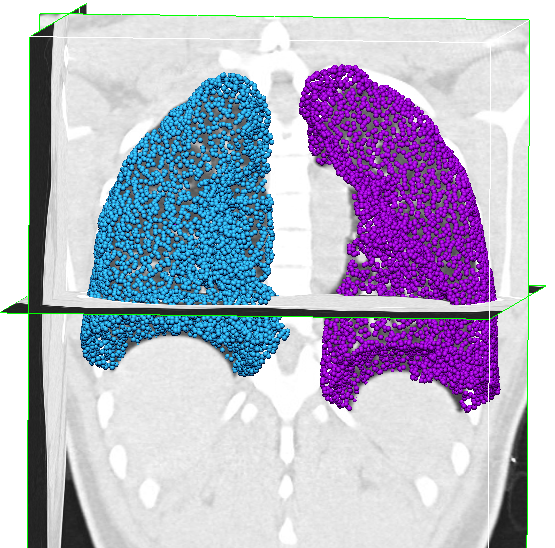
\includegraphics{Segmentation/Image/LungDigitising.png}} 
  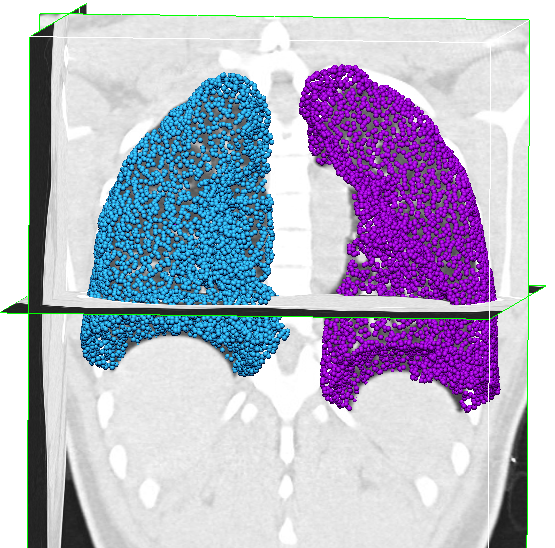
\includegraphics[width=\linewidth,trim={{.0\wd0} {.0\wd0} {.0\wd0} {.0\wd0}},clip]{Segmentation/Image/LungDigitising.png} %trim={<left> <lower> <right> <upper>}, set the cut scale
  \caption{}
  \label{fig:LobeShapeGenereation-a} 
\end{subfigure} 
%\vspace{.3in} % control space between the upper context and figure
\hspace{.3in} % control space between two figures
\begin{subfigure}{.325\linewidth}% set image scale
  \sbox0{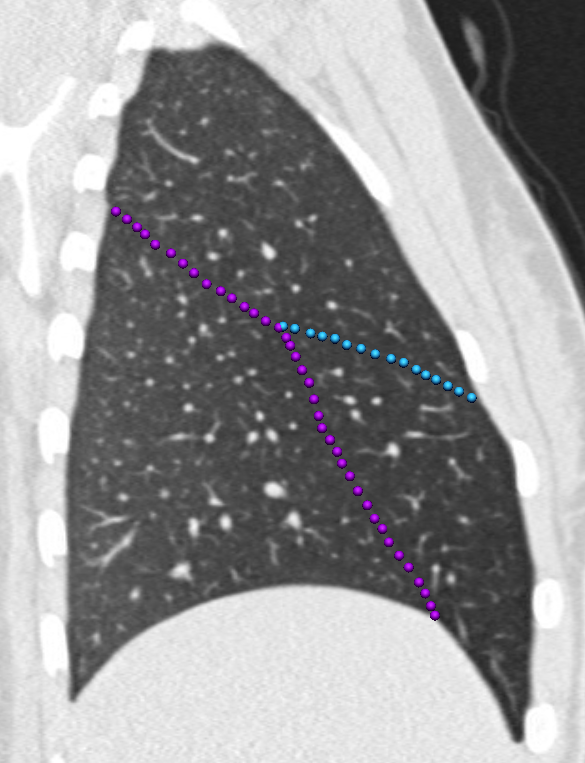
\includegraphics{Segmentation/Image/FissureDigitising1.png}}
  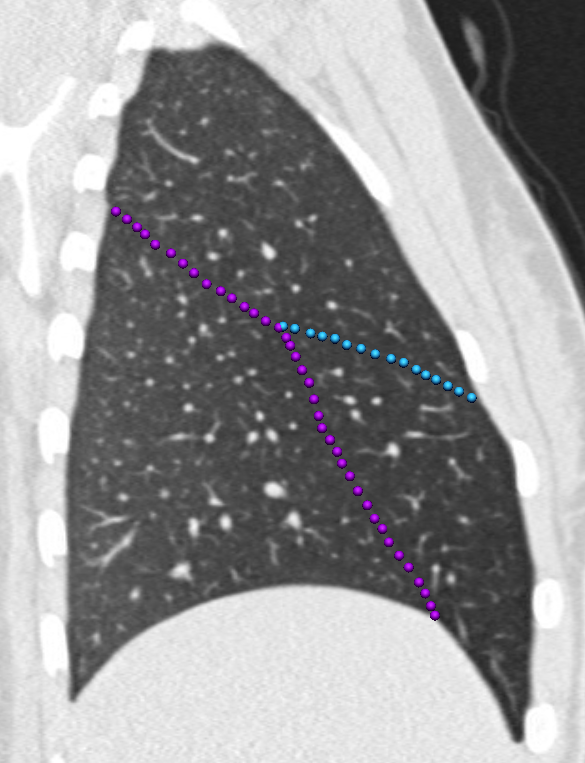
\includegraphics[width=\linewidth,trim={{.0\wd0} {.0\wd0} {.0\wd0} {.0\wd0}},clip]{Segmentation/Image/FissureDigitising1.png}
  \caption{}
  \label{fig:LobeShapeGenereation-b} 
\end{subfigure}
\begin{subfigure}{.48\linewidth}% set image scale
  \sbox0{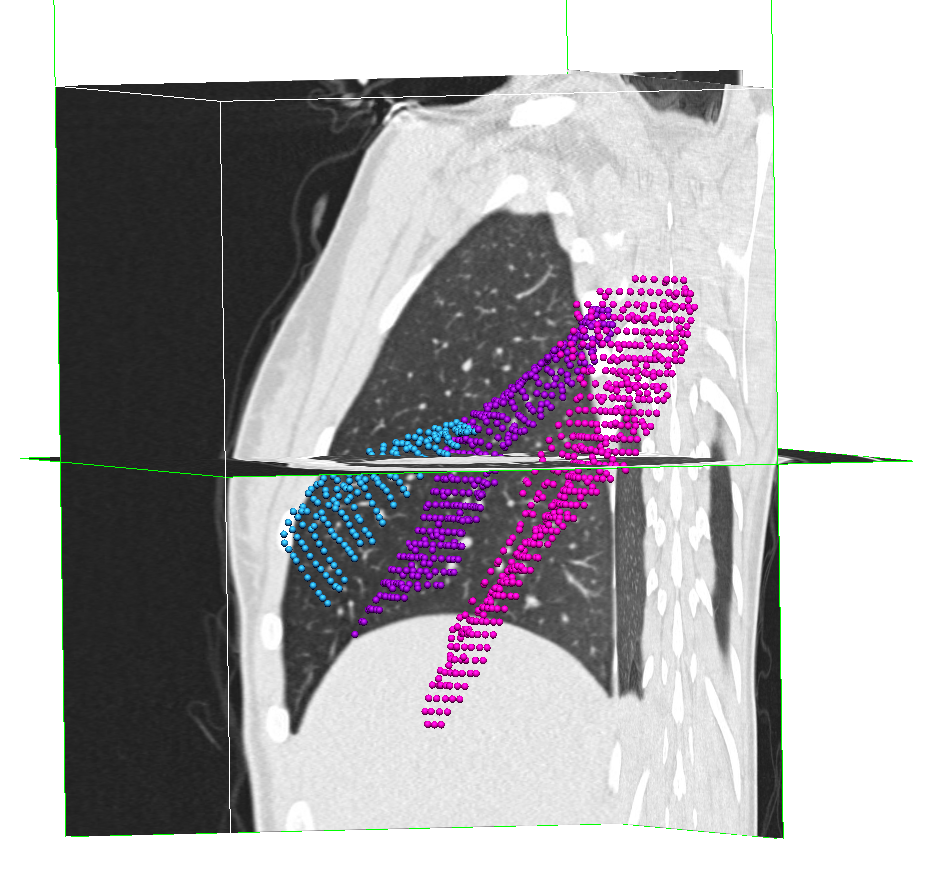
\includegraphics{Segmentation/Image/LobeDigitising.png}}
  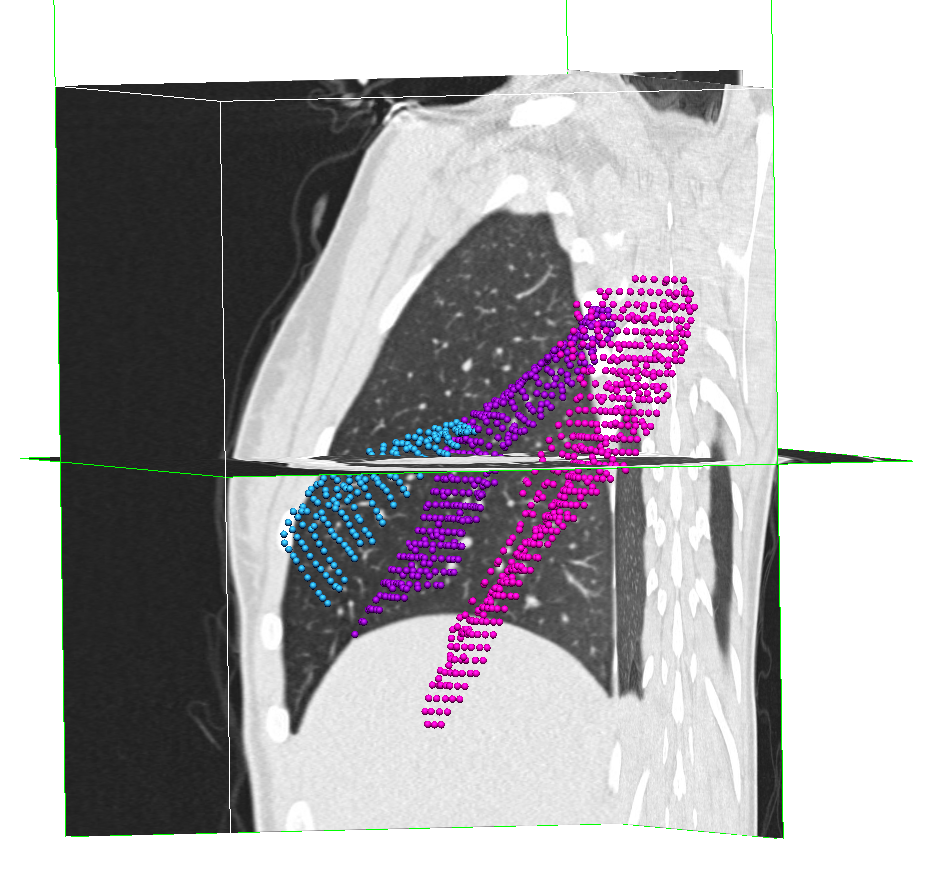
\includegraphics[width=\linewidth,trim={{.0\wd0} {.0\wd0} {.0\wd0} {.0\wd0}},clip]{Segmentation/Image/LobeDigitising.png}
  \caption{}
  \label{fig:LobeShapeGenereation-c} 
\end{subfigure}
%\vspace{.3in} % control space between the upper context and figure
\hspace{.3in} % control space between two figures
\begin{subfigure}{.32\linewidth}% set image scale
  \sbox0{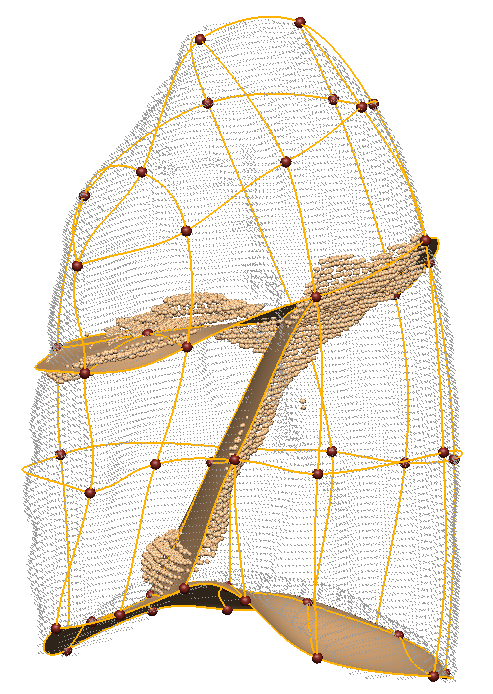
\includegraphics{Segmentation/Image/LobeFitting2.png}}
  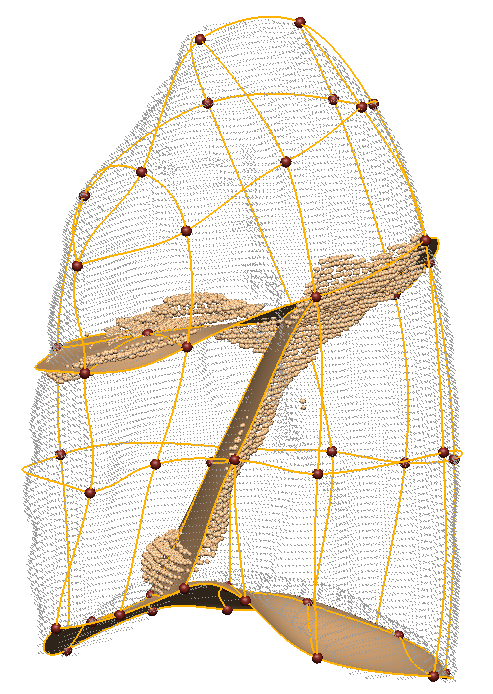
\includegraphics[width=\linewidth,trim={{.0\wd0} {.0\wd0} {.0\wd0} {.0\wd0}},clip]{Segmentation/Image/LobeFitting2.png}
  \caption{}
  \label{fig:LobeShapeGenereation-d} 
\end{subfigure}
\caption{Finite element modeling of lung lobe shape. (a) Lung surface data extracted from segmented lung masks (purple points for left lung, blue points for right lung). (b) Manual digitized fissure points in 2D sagittal image of right lung (purple points for right oblique fissure, blue points for right horizontal fissure). (c) Manual digitized fissure points shown in 3D (pink points for left oblique fissure, purple points for right oblique fissure, blue points for right horizontal fissure). (d) Lobe shape fitting with lung surface data and digitized fissure data of right lung.}
\label{fig:LobeShapeGenereation}
\end{figure}

%%%%%%%%%%%%%%%%%%%%%%%%%%%%%%%%%
\subsubsection{PCA-based statistical shape model construction} \label{SSMConstruction}

A prerequisite of the construction of an SSM is object alignment to remove the orientation and scaling differences between shapes. Here a \gls{gpa} was selected as a registration method \citep{dryden1998statistical,rohlf1999shape}. The GPA algorithm finds the optimal rotation matrix and translation vector which minimizes the overall distance between two sets of points with respect to the Euclidean norm. In this study, a reference lung model sample was randomly chosen from the training set. Then all the other training models were aligned to this reference model. In this process, the volumes of all subjects were normalized to 1 L and any residual rotation and translation were removed. The generalized procrustes alignment can be represented as an affine transformation in mathematical terms

\begin{equation}
 \label{eq:PCAConstruction1}
 \bar{S} = \alpha RS + T,
\end{equation}

\noindent where $\bar{S}$ represents the aligned shape vector to the reference shape from the subject shape vector S, R is the rotation matrix and T is the translation vector. Figure \ref{fig:PCAMeshTraining-a} shows the procrustes aligned meshes of all the 50 subjects. For each subject, the aligned lung shape can also be represented as 

\begin{equation}
 \label{eq:PCAConstruction2}
 \bar{S} = [\mathbf{\bar{x}}_1 \; \mathbf{\bar{x}}_2 \; \mathbf{\bar{x}}_3 \; \cdots \; \mathbf{\bar{x}}_{p-1}; \mathbf{\bar{x}}_p],
\end{equation}

\noindent where $\bar{x}$ are the nodal parameters which contain coordinates and derivatives (12 \gls{dof}s), and p represents the number of nodes for both left and right lung (p = 225 in this study). The data vector $\bar{S}$ of each lung was then assembled as the concatenation of all lungs, termed $\bar{S}_{whole}$. $\bar{S}_{whole}$ is an n$\times$N matrix, where n is the number of nodal parameters for each lung (n = 12 $\times$ 225 = 2700 in this study), and N is the number of training subjects (N = 50). Thus, $\bar{S}_{whole}$ can be regarded as a cloud of N points in the constructed n-N space. This matrix was decomposed into modes of variation using \gls{pca}. \gls{pca} is a commonly used technique in statistical feature space to reduce the dimension of the dataset. It uses an orthogonal transformation to convert a number of (possibly) correlated variables into a set of values of linearly uncorrelated variables called principal components. The number of distinct principal components is equal to the smaller of the number of original variables or the number of observations minus one. The resulting vectors are an uncorrelated orthogonal basis set. 

In order to perform PCA, each shape parameter was centred by subtracting the mean value $\mathbf{\bar{x}}$. Then the covariance matrix was built based on the mean-centred matrix S by $C = SS^T$. After the PCA technique was performed on the covariance matrix C, we obtain a set of eigenvectors $\mathbf{u}_1$, $\mathbf{u}_2$,..., corresponding to a set of non-negative eigenvalues $\lambda_1$, $\lambda_2$,... . Each eigenvalue represents how much variation or variance in the data is captured by the corresponding eigenvector. Each lung shape variation $m_i(w)$ can be approximated by a linear combination of the eigenvector and its corresponding eigenvalue

\begin{equation}
 \label{eq:PCAConstruction3}
 m_i(w) \approx S_{mean} + \mathbf{u}_i w_i,
\end{equation}

\noindent where $w_i$ is a weight factor given to each mode of variation, and i = 1,...,L (L$\leq$ 49 in this study). $S_{mean}$ is the average shape across all the subjects, which is obtained by

\begin{equation}
 \label{eq:PCAConstruction4}
 S_{mean} = \frac{1}{N}\sum_{i=1}^N s_i,
\end{equation}

 \noindent where $s_i$ is the ith lung shape model from the training set, here i = 1,...,N (N=50 in this study). The average shape model is shown in Figure \ref{fig:PCAMeshTraining-b}.

\begin{figure}[htbp] 
\centering
\begin{subfigure}{.4\linewidth}% set image scale
  \sbox0{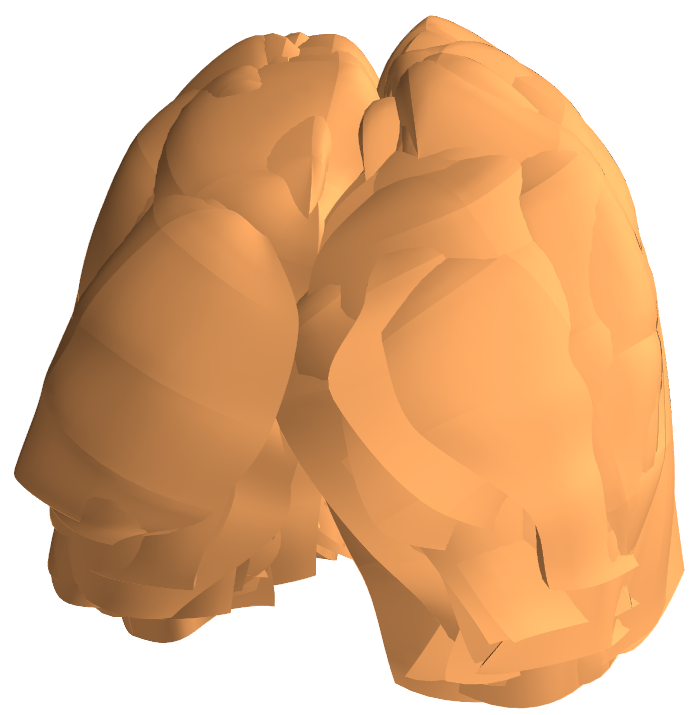
\includegraphics{Segmentation/Image/ProcrustedMeshes.png}}
  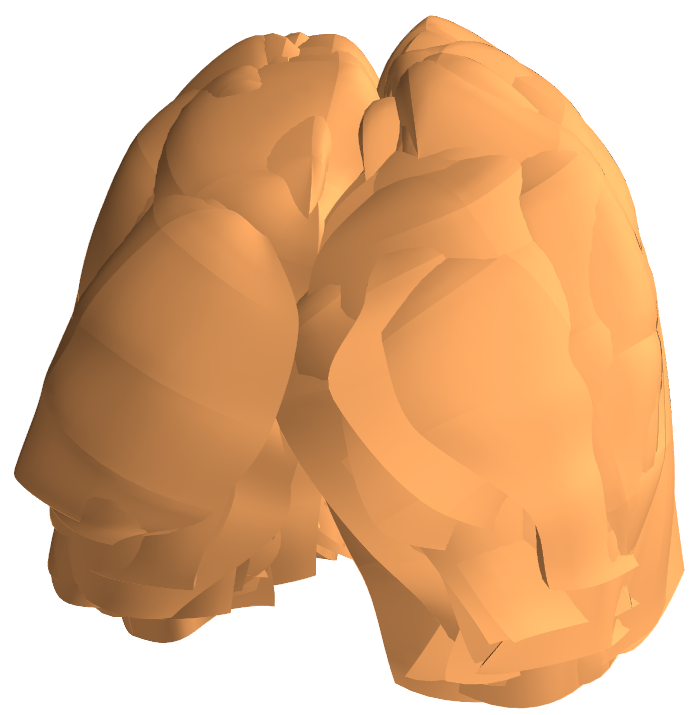
\includegraphics[width=\linewidth,trim={{.0\wd0} {.0\wd0} {.0\wd0} {.0\wd0}},clip]{Segmentation/Image/ProcrustedMeshes.png}
  \caption{}
  \label{fig:PCAMeshTraining-a} 
\end{subfigure}
%\vspace{.3in} % control space between the upper context and figure
\hspace{.3in} % control space between two figures
\begin{subfigure}{.4\linewidth}% set image scale
  \sbox0{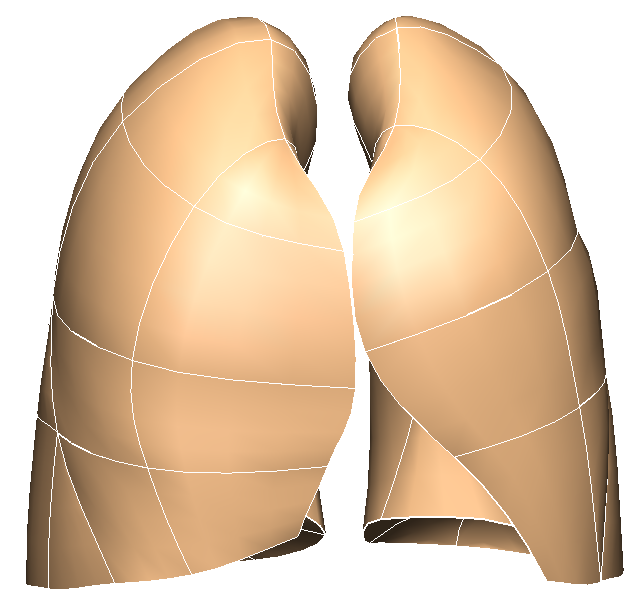
\includegraphics{Segmentation/Image/PCAAverageModel.png}}
  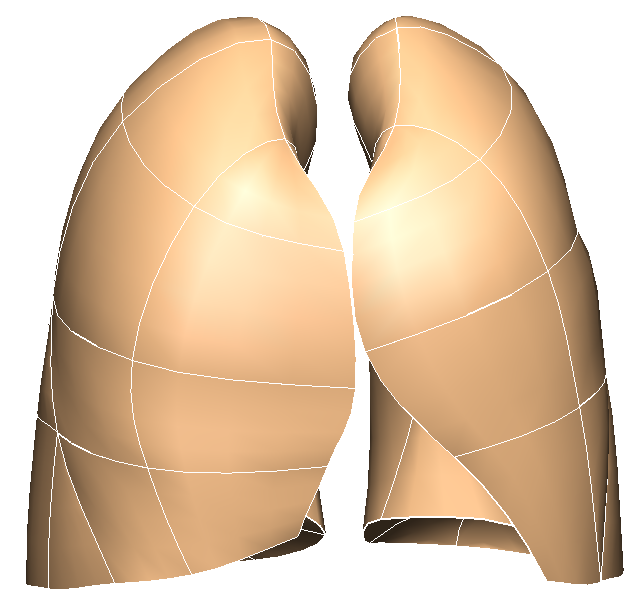
\includegraphics[width=\linewidth,trim={{.0\wd0} {.0\wd0} {.0\wd0} {.0\wd0}},clip]{Segmentation/Image/PCAAverageModel.png}
  \caption{}
  \label{fig:PCAMeshTraining-b} 
\end{subfigure}
\caption{Statistical shape model construction based on principal component analysis. (a) Procrustes aligned meshes of 50 subjects. (b) Average shape model of 50 training subjects. All the weight values are zero for this shape model.}
\label{fig:PCAMeshTraining}
\end{figure}

%%%%%%%%%%%%%%%%%%%%%%%%%%%%%%%%%%%%%%%%%%%%%%%%%%%%%%%
\subsection{Initial prediction of lobar location in an individual} \label{MeshPrediction}

Using the method described in section \ref{ShapeModelGeneration}, the lung shape variation across the training set can be decomposed into a series of modes, and each specific lung shape can be represented with the corresponding mode weight values. In this study each mode represents one type of lung and fissure surface shape variation. In order to predict the fissure location, two PCA-based SSMs were constructed using the same training dataset. The first lobe SSM was built using both the lung surface parameters and fissure surface parameters. The second lung SSM was derived for the same training set but did not include the fissure surfaces and so only described the shape of the lung surface.

The two SSMs were used to predict the fissure locations for subjects that were not part of the training set, using only the definition of the lung surface for the subject as input. A finite element mesh of the lung surface (without fissure information) was generated for each new subject. The new fitted lung mesh was procrustes aligned to the same reference model as the training subjects were aligned to. Then this aligned lung surface mesh was projected on to the lung surface SSM (with no fissure surfaces). The principal component weight values were calculated from the projection, which was represented as $w_{new} = [w_{new1}, w_{new2}, ..., w_{newL}]$ (L$\leq$ 49) here. The first seven principal components accounted for over 90\% of the total lung shape variation in the training set. Therefore, the first seven mode weights were used on the lobe SSM ( which includes both lung and fissure surfaces) to reconstruct the projected lobe mesh for this new subject

\begin{equation}
 \label{eq:FissurePrediction1}
 S_{new} = S_{mean} + \sum_{i=1}^7 \mathbf{u}_i w_{newi},
\end{equation}

\noindent where $S_{mean}$ is the average lobe shape model across all the subjects, $\mathbf{u}_i$ is the first seven eigenvectors of the covariance matrix C corresponding to the lobe \gls{ssm}, and $w_{newi}$ is the projected weight values from the lung \gls{ssm}. An initial estimation of fissure locations was then made (Figure \ref{fig:PCAFissurePrediction}). This initial prediction of lobar fissures provides a reduced search area for subsequent image analysis and ensures an estimation of complete lobar structures even if a fissure is incomplete or is difficult to detect.

\begin{figure}[htbp] 
\centering
\begin{subfigure}{.35\linewidth}% set image scale
  \sbox0{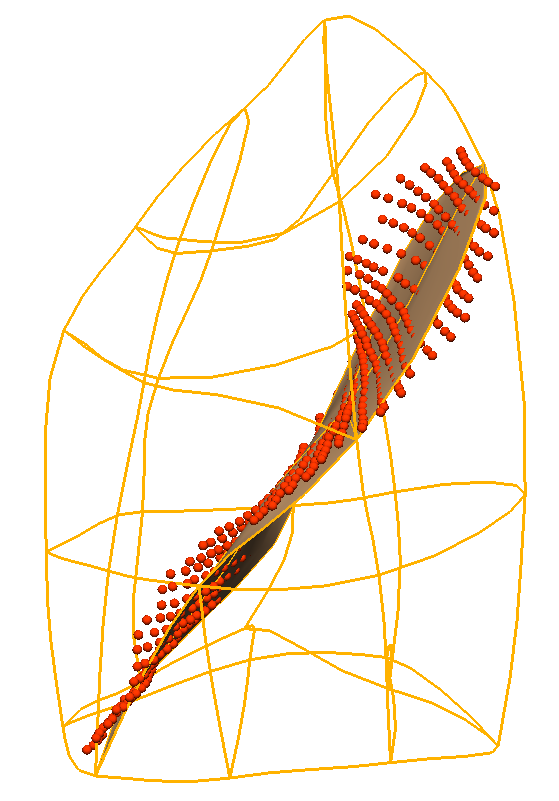
\includegraphics{Segmentation/Image/ProjectedLeftFissureMesh.png}}
  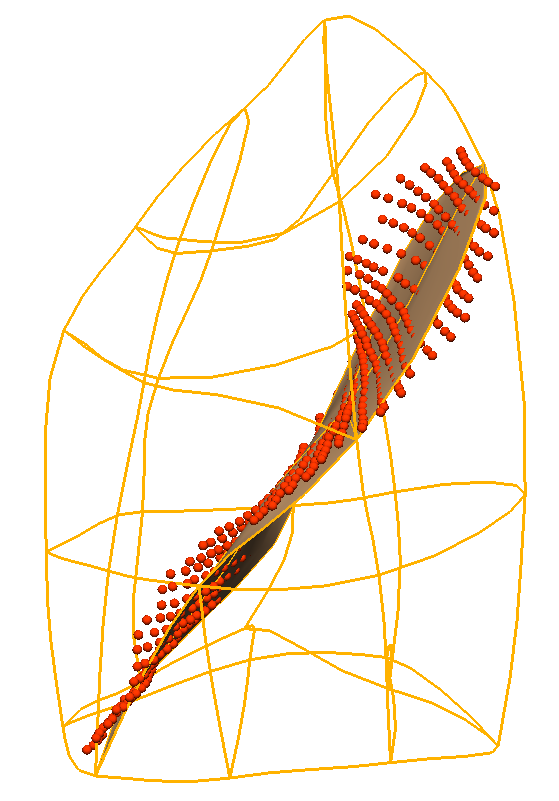
\includegraphics[width=\linewidth,trim={{.0\wd0} {.0\wd0} {.0\wd0} {.0\wd0}},clip]{Segmentation/Image/ProjectedLeftFissureMesh.png}
  \caption{}
  \label{fig:PCAFissurePrediction-a} 
\end{subfigure}
\begin{subfigure}{.37\linewidth}% set image scale
  \sbox0{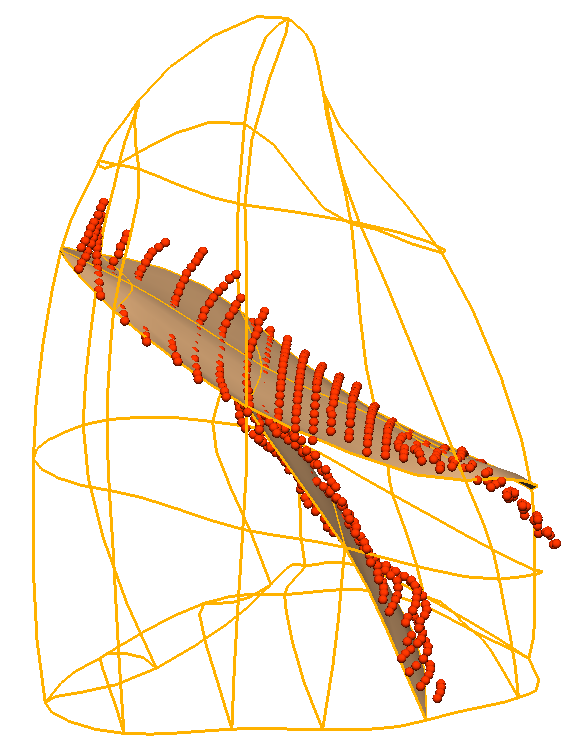
\includegraphics{Segmentation/Image/ProjectedRightFissureMesh.png}}
  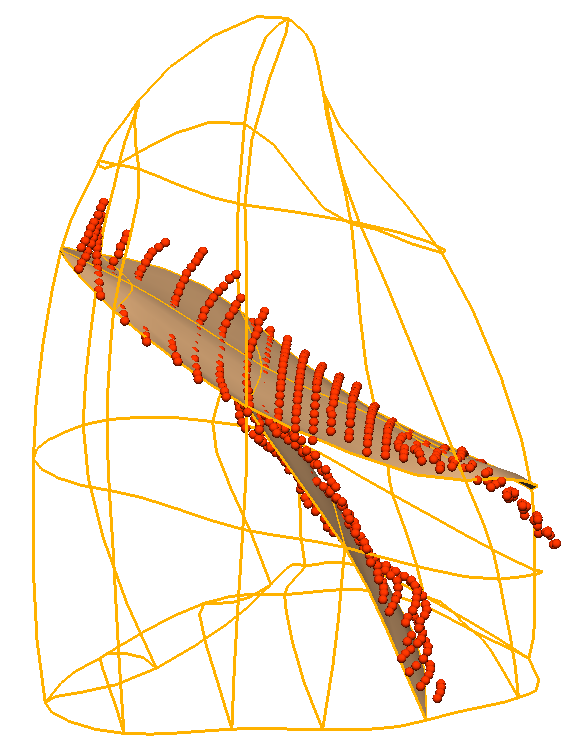
\includegraphics[width=\linewidth,trim={{.0\wd0} {.0\wd0} {.0\wd0} {.0\wd0}},clip]{Segmentation/Image/ProjectedRightFissureMesh.png}
  \caption{}
  \label{fig:PCAFissurePrediction-b} 
\end{subfigure}
\caption{Fissure prediction results compared to ground truth fissure points for one subject. The fissure surface meshes are estimated fissure locations and the red points are manual tracing fissure points by an expert. (a) Left lung. (b) Right lung.}
\label{fig:PCAFissurePrediction}
\end{figure}
%%%%%%%%%%%%%%%%%%%%%%%%%%%%%%%%%%%%%%%%%%%%%%%%%%%%%%%
\subsection{Multi-scale Hessian-based fissure detection}

The final fissure detection was accomplished using an enhancement filter. Conventional enhancement filters are typically based on first (structure tensor) or second (Hessian matrix) order image information \citep{frangi1998multiscale,lorenz1997multi}. This study used the Hessian matrix based on gray-scale curvature information combined with Gaussian smoothing as a basic operator to enhance the fissure structure. In 3D space, fissures are free-form surfaces in the lungs that locally resemble plate-like structures, since the grey-value increases rapidly from the structure border to the centre and decreases again to the opposite border. Hessian-based filters are typically used to enhance and differentiate structures with specific shapes, i.e., blobs, sheets and tubes \citep{frangi1998multiscale,lorenz1997multi}.

A common approach to analyse the local behaviour of an image, L, is to consider the local grey-value variations in the neighbourhood of a point $x_0$ modelled by a Taylor expansion to the second order

\begin{equation}
 \label{eq:FissureDetection1}
 L(x_o + \delta x_o, s) \approx L(x_o, s) + \delta{x_o}^T\nabla_{o,s} + \delta{x_o}^TH_{o,s}\delta x_o,
\end{equation}

\noindent where $\nabla_{o,s}$ and $H_{o,s}$ are the gradient vector and Hessian matrix, respectively, of the image computed in $x_o$ at scale s.

To calculate these differential operators of L, concepts of linear scale space theory are used \citep{koenderink1984structure,florack1992scale}. In this framework, differentiation is defined as a convolution with derivatives of Gaussians

\begin{equation}
 \label{eq:FissureDetection2}
 \pd{L(x,s)}{x} = s^\gamma L(x)*\pd{G(x,s)}{x},
\end{equation}

\noindent where the D-dimensional Gaussian is defined as

\begin{equation}
 \label{eq:FissureDetection3}
 G(x,s) = \frac{1}{{\sqrt{2\pi s^2}}^D}e^{-\frac{{\lVert x \rVert}^2}{2x^2}},
\end{equation}

\noindent where s is the kernel size of the Gaussian. The second derivative of a Gaussian is in many cases a good approximation to the optimal filter for a plane-like structure. Through using the second derivative operator combined with Gaussian smoothing as the basic operator (Hessian matrix), we are able to make the non-supervised fissure filter scale-dependent \citep{lorenz1997multi, li2003selective}. In order to make sure a variety of sizes of fissures can be captured by the Hessian, a range of kernel sizes was implemented from 0.5 mm to 2.5 mm in 0.5 mm increments as the kernel size of the Gaussian to obtain a final estimate of 'fissureness'

\begin{equation}
\label{eq:Multiscale}
F_{output} = \operatorname*{max}\limits_{s_{min}\leq s \leq s_{max}} F_0 (s),
\end{equation}

\noindent where $s_{min}$ and $s_{max}$ are the minimum scale (0.5 mm) and maximum scale (2.5 mm). Each scale s gets a response. In the final output of the multiscale enhancement filter, the maximum output over all scales is assigned to each voxel.

At each image voxel, the Hessian matrix was constructed from the six independent second order derivatives as a symmetric matrix

\begin{equation}
 \label{eq:FissureDetection4}
 Hessian = \begin{bmatrix} H_{xx} & H_{xy} & H_{xz} \\ H_{yx} & H_{yy} & H_{yz} \\ H_{zx} & H_{zy} & H_{zz} \\ \end{bmatrix},
\end{equation}

\noindent where $H_{ij} = \begin{vmatrix} \pd[2]{H}{r_i r_j} \\ \end{vmatrix}$, and r represents the gradient direction.

The idea behind eigenvalue analysis of the Hessian is to extract the principal directions in which the local second order structure of the image can be decomposed. The eigenvalue decomposition extracts three orthonormal directions which are invariant up to a scaling factor when mapped by the Hessian matrix. In this chapter, $\lambda_k$ will be the eigenvalue with the k-th smallest magnitude ($\mid\lambda_{1}\mid\leq\mid\lambda_{2}\mid\leq\mid\lambda_{3}\mid$). Under this assumption, Table \ref{tab:Hessian-based eigenvalue analysis} summarizes different structures distinguished by an analysis of the eigenvalues of the Hessian.

\begin{table}[h]
\centering
\caption{Possible structures on images in 2D and 3D, and its corresponding eigenvalues $\lambda_k$. H and L describe the absolute value of $\lambda_k$, H is high, L is low, +/- indicate the sign of the eigenvalue. The eigenvalues relationship here is: $\mid\lambda_{1}\mid\leq\mid\lambda_{2}\mid\leq\mid\lambda_{3}\mid$.}
\label{tab:Hessian-based eigenvalue analysis}
\begin{tabular}{c c | c c c | c}
\hline
\multicolumn{2}{c|}{\bf{2D}} & \multicolumn{3}{c|}{\bf{3D}} & \bf{Orientation structure}\\ 
\hline
$\lambda_1$ & $\lambda_2$ &  $\lambda_1$ & $\lambda_2$ & $\lambda_3$ &  \\
\hline
   L      &     L     &      L     &     L     &      L     & noisy structure \\
          &           &      L     &     L     &      H-    & bright plane-like structure \\
          &           &      L     &     L     &      H+    & dark plane-like structure \\
   L      &     H-    &      L     &     H-    &      H-    & bright tubular-like structure \\
   L      &     H+    &      L     &     H+    &      H+    & dark tubular-like structure \\
   H-     &     H-    &      H-    &     H-    &      H-    & bright blob-like structure \\	
   H+     &     H+    &      H+    &     H+    &      H+    & dark blob-like structure \\												
\hline
\end{tabular}
\end{table}

As shown in Table \ref{tab:Hessian-based eigenvalue analysis}, an eigenvector analysis of the Hessian matrix can thus be used to detect fissure-like structures, and the respective eigenvectors point out singular directions. In 3D space, a light plane on a dark background is characterized by one large positive second derivative ($\lambda_3$) perpendicular to the fissure plane, since the grey-value increases rapidly from the plane-structure border to the centreline and decreases again to the opposite border. And two small second derivatives of either sign ($\lambda_1$ and $\lambda_2$) parallel to the plane should occur (shown in Fig \ref{fig:FissureHessianEigenvector}). Thus, on the bright fissures, the ideal relationship is defined as $\mid\lambda_{1}\mid = \mid\lambda_{2}\mid = 0$ and $\lambda_{3} \ll 0$, $\mid\lambda_{1}\mid\leq\mid\lambda_{2}\mid\leq\mid\lambda_{3}\mid$. From these characteristics, we can get a fissure probability of each voxel defined as

\begin{equation}
\label{eq:FissureHessian1}
F_0(s) = \Theta S_{plane} S_{noise}.
\end{equation}

The parameter $\Theta$ supresses points whose largest eigenvalue $\lambda_{3}$ is positive, since fissures are locally bright , and is defined as

\begin{equation}
\label{eq:FissureHessian2}
\Theta = \begin{cases}
         1,\quad \lambda_{3}< 0\\,
         0, \quad \lambda_{3}\geq0.
         \end{cases}
\end{equation}

Since the largest eigenvalue $\mid\lambda_{3}\mid$ should be much larger than the other two eigenvectors, the second factor $S_{plane}$ uses the ratio between $\mid\lambda_{2}\mid$ and $\mid\lambda_{3}\mid$ to search sheet-like structures, so that the voxels where $\mid\lambda_{3}\mid$ and $\mid\lambda_{2}\mid$ are significantly different. $S_{plane}$ is defined as

\begin{equation}
\label{eq:FissureHessian3}
S_{plane} = exp(-\frac{{R_{plane}}^2}{2\alpha^2}), \\
\end{equation}

\begin{equation}
\label{eq:FissureHessian4}
R_{plane} = \frac{\mid\lambda_{2}\mid}{\mid\lambda_{3}\mid},
\end{equation}

\noindent where $\alpha$ was set to 0.5 in this study. The third factor $S_{noise}$ aims to suppress noise voxels such as blob-like structures. Unlike plane-like structures which have relatively large $\mid\lambda_{2}\mid$ and $\mid\lambda_{3}\mid$ ratio, the noise voxels usually have low $\mid\lambda_{1}\mid$, $\mid\lambda_{2}\mid$ and $\mid\lambda_{3}\mid$ (as shown in Table \ref{tab:Hessian-based eigenvalue analysis}). Therefore, here we use

\begin{equation}
\label{eq:FissureHessian5}
S_{noise} = 1 - exp(-\frac{{R_{noise}}^2}{2\beta^2}), \\
\end{equation}

\begin{equation}
\label{eq:FissureHessian6}
R_{noise} = \sqrt{{\lambda_1}^2+{\lambda_2}^2+{\lambda_3}^2},
\end{equation}

\noindent with $\beta$ set to 0.5 for thresholding. $F_0(s)$ then gives a high response to local plane-like structures (fissures) and suppresses other pulmonary structures (noise). An example of this enhancement filter applied in an individual is shown in Figure \ref{fig:FissureDetection-a}. 

\begin{figure*}[htbp]
  \centering 
	\vspace{.15in} % control space between the upper context and figure
  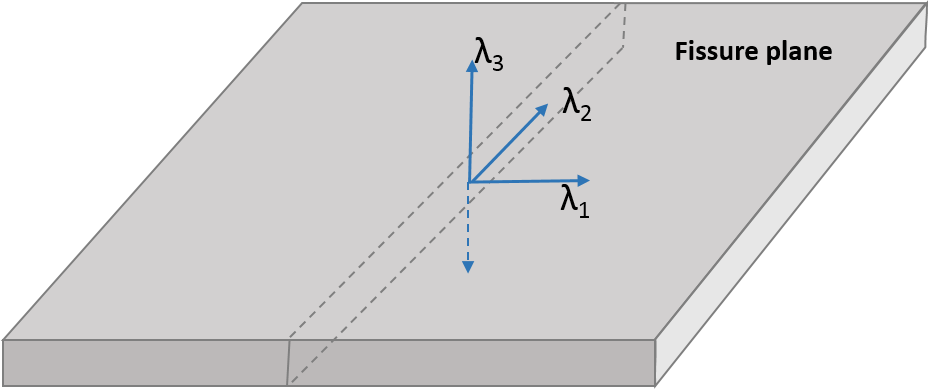
\includegraphics[height=1.5in]{Segmentation/Image/FissureHessianEigenvector.png}
  \caption{The three eigenvectors of the Hessian matrix representing plane-like structure (fissure). $\lambda_1$ and $\lambda_2$ are parallel to fissure plane, $\lambda_3$ is perpendicular to fissure plane.}
  \label{fig:FissureHessianEigenvector}
\end{figure*}

Blood vessel voxels were subsequently filtered from the fissure enhanced result. The segmentation of vessels was achieved using a classical vessel segmentation method \citep{frangi1998multiscale}. This method uses a multiple scale (from 0.5 mm to 3.0 mm in 0.5 mm increments as the kernel size of Gaussian) Hessian-based enhanced filter, which is similar to the fissure detection filter described previously. The main difference is here the aim is to search for the tube structure (vessels). In a 3D image,  the relationship of Hessian eigenvalues $\lambda_{1}$, $\lambda_{2}$ and $\lambda_{3}$ of an ideal bright tubular structure in a dark background should be described as $\mid\lambda_{1}\mid\approx$ 0, $\mid\lambda_{1}\mid\ll\mid\lambda_{2}\mid$,  $\lambda_{2}\approx\lambda_{3}$ (see Figure \ref{fig:VesselHessianEigenvector}). Therefore, the following equations were used as the enhancement filter to detect vesselness structures

\begin{equation}
\label{eq:VesselHessian1}
V_0(s) = \begin{cases}
         0,\quad\quad\quad\quad\quad\quad\quad if \quad \lambda_{2}>0,\\
         (1-exp(-\frac{{R_A}^2}{a^2}))exp(-\frac{{R_B}^2}{2b^2})(1-exp(-\frac{S^2}{2c^2})),
         \end{cases}
\end{equation}

\noindent where a and b were both set to 0.5, and c was set to 500 in this study. $R_A$, $R_B$ and S are defined as

\begin{equation}
\label{eq:VesselHessian2}
R_A = \frac{\mid\lambda_{2}\mid}{\mid\lambda_{3}\mid}, 
\end{equation}

\begin{equation}
\label{eq:VesselHessian3}
R_B = \frac{\mid\lambda_{1}\mid}{\sqrt{\mid\lambda_{2}\mid \mid\lambda_{3}\mid}},
\end{equation}

\begin{equation}
\label{eq:VesselHessian3}
S = {\Vert H \rVert}_F = \sqrt{\sum_{j\leq D}}{\lambda_j}^2,
\end{equation}

\noindent where $D$ is the dimension of the image. $V_0(s)$ gives a probability of vesselness for each voxel. Then segmented blood vessels were selected through detecting the voxels whose vesselness value was larger than a specific threshold (threshold = 10 in this study \citep{frangi1998multiscale}). $D{vessel}$ was used to represent the distance transform to the segmented vessel line, thus the final fissureness after decreasing the values of vessel voxels was defined as

\begin{equation}
\label{eq:FinalFissureness}
F_{final}(s) = F_0(s)S_{vessels},
\end{equation}

\begin{equation}
\label{eq:FinalFissureness}
S_{vessels} = exp(1-\frac{{D{vessel}}^2}{2d^2}),
\end{equation}

\noindent  where $d$ was set to 5mm in this study. High vesselness voxels were therefore suppressed and not detected as fissure points in the final result. Fig \ref{fig:FissureDetection-b} shows the result after eliminating the vessel voxels.

\begin{figure*}[htbp]
  \centering 
  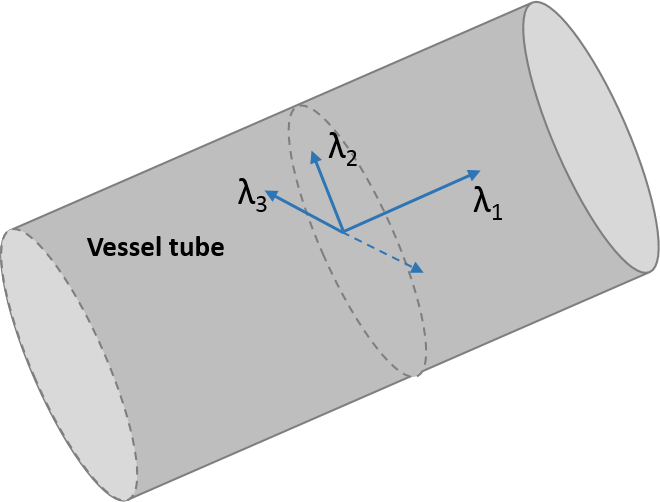
\includegraphics[height=1.5in]{Segmentation/Image/VesselHessianEigenvector.png}
  \caption{The three eigenvectors of the Hessian matrix representing tube-like structure (vessel). $\lambda_1$ is parallel to vessel tube, $\lambda_2$  and $\lambda_3$ are perpendicular to vessel tube.}
  \label{fig:VesselHessianEigenvector}
\end{figure*}

The initial fissure location predicted by average SSM deformation gives a region of interest (ROI) for an accurate fissure detection, see Figure \ref{fig:FissureDetection-c}. The candidate points are selected within a certain distance of the initial fissure approximation: the search distance was set to 20 voxels (default value) for the initially projected left and right oblique fissures and 15 voxels for the initially projected right horizontal fissure. To remove some spurious responses such as small plane-like structures on the result, a 2D 4-neighbourhood connected component filter and a 3D 6-neighbourhood vector-based connected component filter were employed successively to eliminate noise arising from small plane-like structures in this search region (Fig \ref{fig:FissureDetection-d}). A 2D filter was used to eliminate 4-neighbour connected components that were smaller than a minimum small size (set to 10 voxels initially) slice by slice. The 3D vector-based connected component filter used the inner product of the normalized largest eigenvector of the Hessian matrix in adjacent voxels. These largest eigenvectors are perpendicular to the fissure plane, and their inner product provides a criterion for component connection. As the curvature of a fissure is locally low, adjacent fissure voxels should have similar largest eigenvectors and thus the inner product value of their largest eigenvectors should equal to 1 or slightly smaller than 1. Connected boundary condition was set as an inner product $\leq$ 0.8 to connected component, then 3D 6-neighbour connected component with a volume less than 100 $\mathrm{mm^3}$ was removed as noise from the result.

The detected points were then divided into a set of small subsections corresponding to different x, y intervals. For each subsection, the point of the highest fissure probability (the highest S value) was selected as the final candidate fissure point (Fig \ref{fig:FissureDetection-e}). Once the maximum fissureness candidates were found, a morphological dilation with a $3\times3\times3$ voxel cube as structure element was applied iteratively until the largest connected fissure plane was big enough, so that all the other unconnected outliers could be filtered subsequently. Finally, a continuous smooth fissure surface was generated based on the maximum fissure points using a $\beta$-spline method with a thin-plane spline \citep{lee1997scattered} and extrapolated to the lung boundaries, see Fig \ref{fig:FissureDetection-f}.

\begin{figure}[htbp] 
\centering
\begin{subfigure}{.41\linewidth}% set image scale
  \sbox0{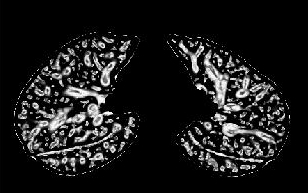
\includegraphics{Segmentation/Image/FissureDetection1.jpg}} 
  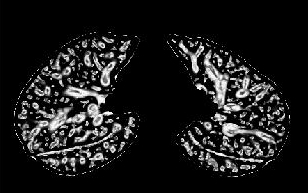
\includegraphics[width=\linewidth,trim={{.0\wd0} {.0\wd0} {.0\wd0} {.0\wd0}},clip]{Segmentation/Image/FissureDetection1.jpg} %trim={<left> <lower> <right> <upper>}, set the cut scale
  \caption{}
	\label{fig:FissureDetection-a}
\end{subfigure} 
\begin{subfigure}{.408\linewidth}% set image scale
  \sbox0{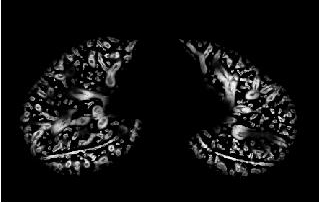
\includegraphics{Segmentation/Image/FissureDetection2.jpg}}
  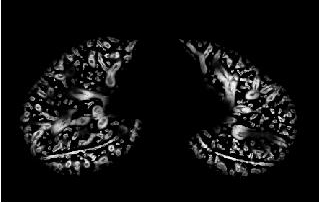
\includegraphics[width=\linewidth,trim={{.0\wd0} {.0\wd0} {.0\wd0} {.0\wd0}},clip]{Segmentation/Image/FissureDetection2.jpg}
  \caption{}
	\label{fig:FissureDetection-b}
\end{subfigure}
\begin{subfigure}{.4\linewidth}% set image scale
  \sbox0{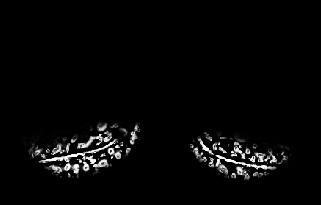
\includegraphics{Segmentation/Image/FissureDetection3.jpg}}
  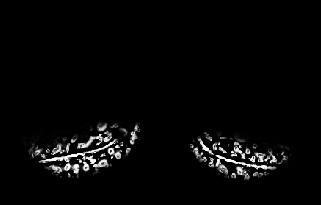
\includegraphics[width=\linewidth,trim={{.0\wd0} {.0\wd0} {.0\wd0} {.0\wd0}},clip]{Segmentation/Image/FissureDetection3.jpg}
  \caption{}
	\label{fig:FissureDetection-c}
\end{subfigure}
\begin{subfigure}{.412\linewidth}% set image scale
  \sbox0{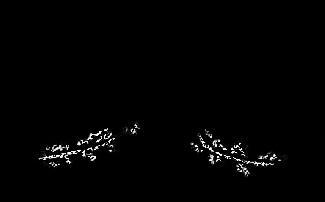
\includegraphics{Segmentation/Image/FissureDetection4.jpg}}
  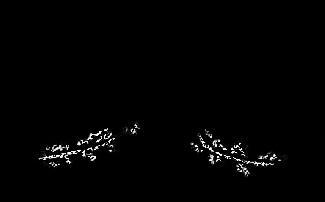
\includegraphics[width=\linewidth,trim={{.0\wd0} {.0\wd0} {.0\wd0} {.0\wd0}},clip]{Segmentation/Image/FissureDetection4.jpg}\label{fig:FissureDetection}
  \caption{}
	\label{fig:FissureDetection-d}
\end{subfigure}
\begin{subfigure}{.41\linewidth}% set image scale
  \sbox0{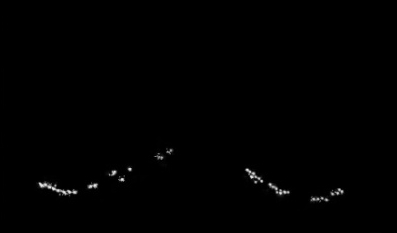
\includegraphics{Segmentation/Image/FissureDetection5.jpg}}
  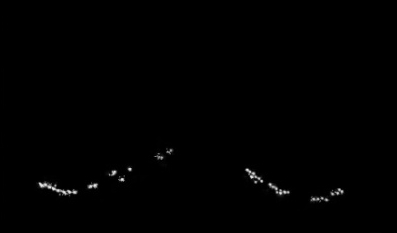
\includegraphics[width=\linewidth,trim={{.0\wd0} {.0\wd0} {.0\wd0} {.0\wd0}},clip]{Segmentation/Image/FissureDetection5.jpg}
  \caption{}
	\label{fig:FissureDetection-e}
\end{subfigure}
\begin{subfigure}{.415\linewidth}% set image scale
  \sbox0{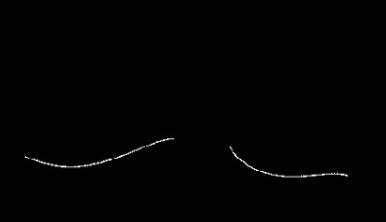
\includegraphics{Segmentation/Image/FissureDetection6.jpg}}
  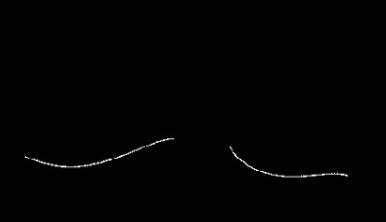
\includegraphics[width=\linewidth,trim={{.0\wd0} {.0\wd0} {.0\wd0} {.0\wd0}},clip]{Segmentation/Image/FissureDetection6.jpg}
  \caption{}
	\label{fig:FissureDetection-f}
\end{subfigure}
\caption{Hessian-based multiscale fissure detection results. (a) Hessian-based plane-like structure enhancement filter. (b) Remove vessel voxels (tube-like structures). (c) Selected search regions for fissure detection based on SSM initial fissure prediction. (d) 2D and 3D eigenvector based connected component filter. (e) Fissure candidate points. (f) $\beta$-spline curve fissure surface fitting.}
\label{fig:FissureDetection}
\end{figure}

%%%%%%%%%%%%%%%%%%%%%%%%%%%%%%%%%%%%%%%%%%%%%%%%%%%%%%%%
\subsection{Interactive user control interface} \label{UserControl}
As discussed above, a series of parameter values need to be chosen correctly to ensure a successful lobar segmentation. However, a fixed parameter value is usually not suitable for all the subjects due to a wide variation of lung tissue and fissure appearances across the population. Therefore, a fast and convenient manual interaction to control the segmentation procedure is reasonable and acceptable. Based on an open source software, Pulmonary Toolkit (PTK, https://github.com/tomdoel/pulmonarytoolkit), an improved user-friendly interactive interface was developed to control the segmentation parameters as input (improved version: https://github.com/qiuyufly/pulmonarytoolkit/tree/yuwen). PTK is a software developed on Matlab for the analysis of 3D medical lung images for academic research use. It comprises a library of lung analysis algorithms, a GUI application for visualising and analysing clinical lung images and a rapid prototyping framework for users to develop their new algorithms in an easy way. By making use of some built-in objects and the visualisation system of PTK, the lobar segmentation algorithm was added into the algorithm package and parameter control buttons were made available on the interface. Table \ref{tab:ParameterUserControl} summarises the interactive user control parameters. Figure \ref{fig:PTKUserInterface} shows the user interface of PTK.

\newcolumntype{C}[1]{>{\centering\arraybackslash}p{#1}}
\begin{table}[htbp]
\centering
\caption{Summary of interactive user control parameters}
\label{tab:ParameterUserControl}
\begin{tabular}{|p{4.5cm}|p{2.3cm}|l|}
\hline
\bf{Parameters} & \bf{Default values} & \bf{Notes}\\ 
\hline
Search region for left oblique fissure & 20 voxels &  \multirow{3}{5.2cm}{Increase the value if there are not enough positive candidate points; decrease the value if there is too much noise} \\
\cline{1-2}
Search region for right horizontal fissure & 20 voxels &  ~ \\
\cline{1-2}
Search region for right oblique fissure & 15 voxels &  ~ \\
\hline
Connected component size for left oblique fissure & 30 voxels &  \multirow{4}{5.2cm}{Decrease the value if there are\\not enough positive candidate points; increase the value if there is too much noise} \\
\cline{1-2}
Connected component size for right horizontal fissure & 30 voxels &  ~ \\
\cline{1-2}
Connected component size for right oblique fissure & 30 voxels &  ~ \\
\cline{1-2}
Total connected component size & 300 voxels &  ~ \\
\hline
\end{tabular}
\end{table}

\begin{figure*}[htbp]
  \flushleft 
  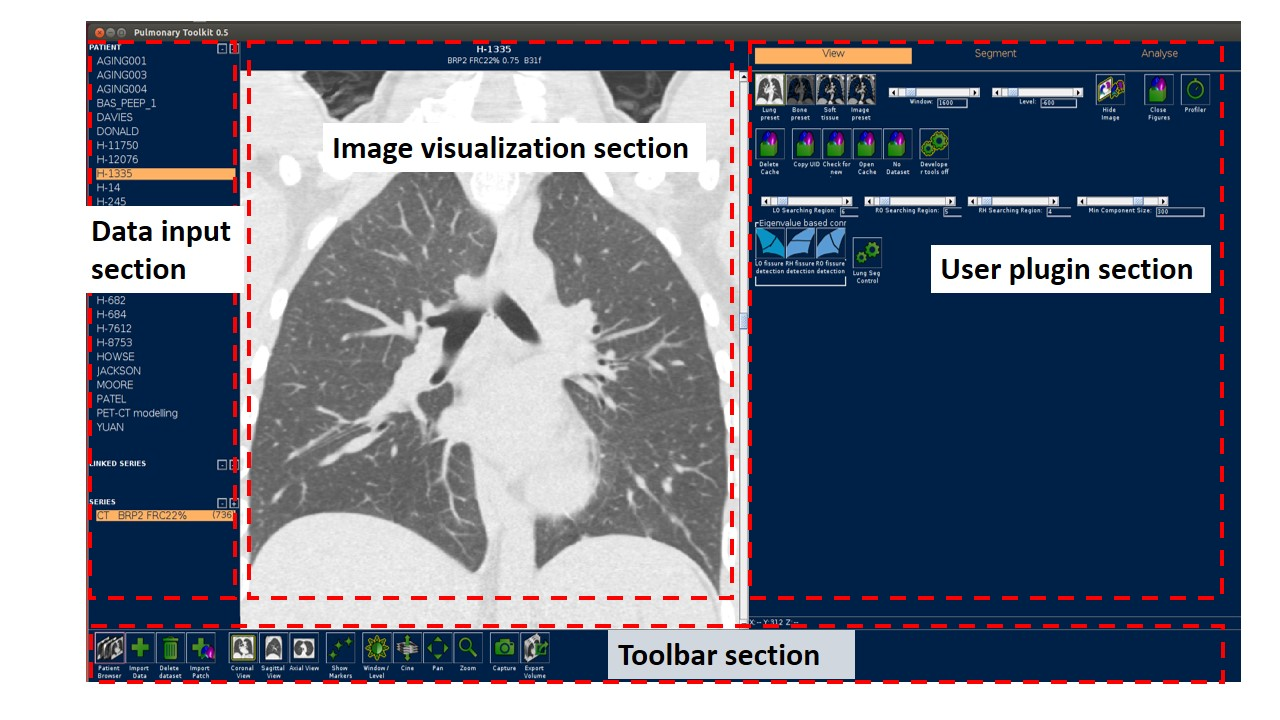
\includegraphics[height=3.2in]{Segmentation/Image/PTKUserInterface.jpg}
  \caption{PTK User interactive interface. It consists of data input section, image visualization section, user plugin section and toolbar section.}
  \label{fig:PTKUserInterface}
\end{figure*}

%%%%%%%%%%% 
\subsubsection{Search region control}
Fissure candidate points were detected within a certain distance of the initial fissure approximation. The default distance was set to 20 voxels for left and right oblique fissures and 15 voxels for right horizontal fissure. However, with a fixed search distance, fissure detection sometimes could not be implemented efficiently and accurately. The probability of error detection may increase if the search distance is too large, as more noise will be included in the initial search region. In contrast some positive fissure points will be missed if the search distance is too small. Accurate fissure candidate points are an important prerequisite for good fissure surface fitting. Therefore, user interactive slide buttons were developed on the PTK interface to control the search distance. Through inputting SSM based initial fissure prediction mesh, the estimated fissures can be  visualized to overlap on the raw images in the PTK visualization section. Then it is possible for users to select a suitable search region for each fissure depending on the accuracy of the initial fissure estimate. The better the initial fissure approximation, the lower the search region that should be selected. Figure \ref{fig:SearchRegionControl} shows the lobe segmentation result before and after change to the search region.
\newpage

\begin{figure}[htbp] 
\centering
\begin{subfigure}{.32\linewidth}% set image scale
  \sbox0{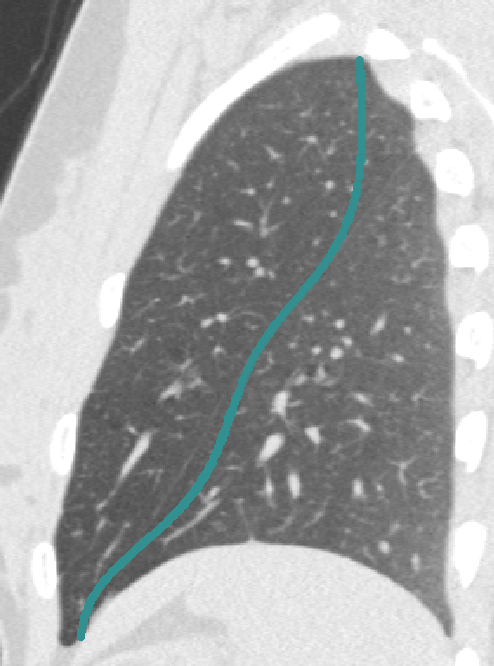
\includegraphics{Segmentation/Image/BeforeChangeSearchRegion.png}}
  \includegraphics[width=\linewidth,trim={{.0\wd0} {.0\wd0} {.0\wd0} {.0\wd0}},clip]{Segmentation/Image/BeforeChangeSearchRegion.png}
  \caption{}
  \label{fig:SearchRegionControl-a} 
\end{subfigure}
%\vspace{.3in} % control space between the upper context and figure
\hspace{.3in} % control space between two figures
\begin{subfigure}{.33\linewidth}% set image scale
  \sbox0{\includegraphics{Segmentation/Image/AfterChangeSearchRegion.png}}
  \includegraphics[width=\linewidth,trim={{.0\wd0} {.0\wd0} {.0\wd0} {.0\wd0}},clip]{Segmentation/Image/AfterChangeSearchRegion.png}
  \caption{}
  \label{fig:SearchRegionControl-b} 
\end{subfigure}
\caption{Fissure detection results before and after control the search regions. (a) Fissure detection result with a search distance of default 20 voxels. (b) Fissure detection result after setting a specific search distance depending on the accuracy of initial fissure guessing.}
\label{fig:SearchRegionControl}
\end{figure}

\subsubsection{Connected component analysis filter control}
Connected component analysis is an important operation to help with noise elimination during fissure detection. A suitable connected component size is able to remove most of the small connected structures as outliers and in the meantime retain true fissure structures as much as possible. In order to improve the filter performance, a slide button was used to control the connected component size on the PTK user interface. Through changing the component size threshold, it is possible for us to find a balance between spurious response elimination and target points retainment. 

\subsubsection{Manual correction}
Manual correction remains an essential part of lobe segmentation processing. A manual correction tool was available in the PTK software, but in this method only one correct landmark could be selected at a time. Here, a multiple landmark correction method was developed based on PTK built-in packages, and the improved correction tool allows users to modify three fissure points at the same time. By selecting a series of correction landmarks, the corresponding fissure plane is deformed to a new curved surface which passes through all the correct landmarks. The correction region was calculated based on the distance between the landmark and its corresponding fissure plane, and a 3D Gaussian filter with the landmark as the centre was also used to specify the corrected boundary. The correction happens in 3D space so that users don't need to do the correction slice by slice. The whole correction can be finished in a few minutes even when automatic fissure is not complete. Figure \ref{fig:ManualCorrection} shows the fissure detection results before and after manual correction.

\begin{figure}[htbp] 
\centering
\begin{subfigure}{.44\linewidth}% set image scale
  \sbox0{\includegraphics{Segmentation/Image/BeforeManualCorrection.png}}
  \includegraphics[width=\linewidth,trim={{.0\wd0} {.0\wd0} {.0\wd0} {.0\wd0}},clip]{Segmentation/Image/BeforeManualCorrection.png}
  \caption{}
  \label{fig:ManualCorrection-a} 
\end{subfigure}
\vspace{.1in} % control space between the upper context and figure
%\hspace{.3in} % control space between two figures
\begin{subfigure}{.44\linewidth}% set image scale
  \sbox0{\includegraphics{Segmentation/Image/AfterManualCorrection.png}}
  \includegraphics[width=\linewidth,trim={{.0\wd0} {.0\wd0} {.0\wd0} {.0\wd0}},clip]{Segmentation/Image/AfterManualCorrection.png}
  \caption{}
  \label{fig:ManualCorrection-b} 
\end{subfigure}
\caption{Manual correction on automatic fissure detection results (a) Manually select a set of landmarks on real fissure lines shown in raw images to correct automatic fissure detection results (red landmarks are for left oblique fissure, green landmarks are for right oblique fissure, blue landmarks are for right horizontal fissure). (b) Corrected fissure detection results shown with raw images. The corrected fissure lines can match the real fissure locations.}
\label{fig:ManualCorrection}
\end{figure}

%%%%%%%%%%%%%%%%%%%%%%%%%%%%%%%%%%%%%%%%%%%%%%%%%%%%%%%
\section{Results for SMM segmentation} \label{SegmentationExperiment}

\subsection{Testing CT dataset}
The semi-automatic SSM lobe segmentation method was tested on two datasets: 1) CT images from five young normal subjects taken at different lung volumes (end inspiration and end expiration), in the supine posture, from the HLA dataset (introduced in Section \ref{ShapeModelGeneration}). The selected dataset consists of five end expiration images and five end inspiration images, which were not part of the SSM training set; 2) CT images from older patients (slice thickness 1.25-3.00 mm) acquired during routine diagnostic inspection for idiopathic pulmonary fibrosis (IPF). Data from these subjects were acquired from the \gls{adhb}. Access to clinical data was approved by the Southern Health and Disability Ethics Committee. 

\subsection{Test and results}
Figure \ref{fig:HLASegmentationResults} shows raw images, initial SSM based fissure predicted locations, and the final automatic SSM-based lobar segmentation results (no manual correction) for a normal healthy subject. Figure \ref{fig:IPFSegmentationResults} shows the results for an IPF subject.

\begin{figure}[htbp] 
\centering
\begin{subfigure}{.25\linewidth}% set image scale
  \sbox0{\includegraphics{Segmentation/Image/H1335_FRC_Raw_Sagittal.png}}
  \begin{overpic}[width=\linewidth,trim={{.0\wd0} {.0\wd0} {.0\wd0} {.0\wd0}},clip]{Segmentation/Image/H1335_FRC_Raw_Sagittal.png}
      \put(16,105){\bf{Raw images}}
			\put(-38,55){\bf{Sagittal}}
  \end{overpic}
  \caption{}
  \label{fig:HLASegmentationResults-a} 
\end{subfigure}
%\vspace{.1in} % control space between the upper context and figure
\hspace{.3in} % control space between two figures
\begin{subfigure}{.25\linewidth}% set image scale
  \sbox0{\includegraphics{Segmentation/Image/H1335_FRC_PCAInitial_Sagittal.png}}
  \begin{overpic}[width=\linewidth,trim={{.0\wd0} {.0\wd0} {.0\wd0} {.0\wd0}},clip]{Segmentation/Image/H1335_FRC_PCAInitial_Sagittal.png}
      \put(0,105){\bf{Initial SSM-based fissures}}
  \end{overpic}
  \caption{}
  \label{fig:HLASegmentationResults-b} 
\end{subfigure}
%\vspace{.1in} % control space between the upper context and figure
\hspace{.3in} % control space between two figures
\begin{subfigure}{.25\linewidth}% set image scale
  \sbox0{\includegraphics{Segmentation/Image/H1335_FRC_PCAFissureDetection_Sagittal.png}}
  \begin{overpic}[width=\linewidth,trim={{.0\wd0} {.0\wd0} {.0\wd0} {.0\wd0}},clip]{Segmentation/Image/H1335_FRC_PCAFissureDetection_Sagittal.png}
      \put(15,105){\bf{Final fissures}}
  \end{overpic}
  \caption{}
  \label{fig:HLASegmentationResults-c} 
\end{subfigure}
\begin{subfigure}{.32\linewidth}% set image scale
  \sbox0{\includegraphics{Segmentation/Image/H1335_FRC_Raw_Axial.png}}
  \begin{overpic}[width=\linewidth,trim={{.0\wd0} {.0\wd0} {.0\wd0} {.0\wd0}},clip]{Segmentation/Image/H1335_FRC_Raw_Axial.png}
			\put(-30,30){\bf{Axial}}
  \end{overpic}
  \caption{}
  \label{fig:HLASegmentationResults-d} 
\end{subfigure}
%\vspace{.1in} % control space between the upper context and figure
%\hspace{.3in} % control space between two figures
\begin{subfigure}{.32\linewidth}% set image scale
  \sbox0{\includegraphics{Segmentation/Image/H1335_FRC_PCAInitial_Axial.png}}
  \includegraphics[width=\linewidth,trim={{.0\wd0} {.0\wd0} {.0\wd0} {.0\wd0}},clip]{Segmentation/Image/H1335_FRC_PCAInitial_Axial.png}
  \caption{}
  \label{fig:HLASegmentationResults-e} 
\end{subfigure}
%\vspace{.1in} % control space between the upper context and figure
%\hspace{.3in} % control space between two figures
\begin{subfigure}{.32\linewidth}% set image scale
  \sbox0{\includegraphics{Segmentation/Image/H1335_FRC_PCAFissureDetection_Axial.png}}
  \includegraphics[width=\linewidth,trim={{.0\wd0} {.0\wd0} {.0\wd0} {.0\wd0}},clip]{Segmentation/Image/H1335_FRC_PCAFissureDetection_Axial.png}
  \caption{}
  \label{fig:HLASegmentationResults-f} 
\end{subfigure}
\begin{subfigure}{.32\linewidth}% set image scale
  \sbox0{\includegraphics{Segmentation/Image/H1335_FRC_Raw_Coronal.png}}
  \begin{overpic}[width=\linewidth,trim={{.0\wd0} {.0\wd0} {.0\wd0} {.0\wd0}},clip]{Segmentation/Image/H1335_FRC_Raw_Coronal.png}
			\put(-35,40){\bf{Coronal}}
  \end{overpic}
  \caption{}
  \label{fig:HLASegmentationResults-g} 
\end{subfigure}
%\vspace{.1in} % control space between the upper context and figure
%\hspace{.3in} % control space between two figures
\begin{subfigure}{.32\linewidth}% set image scale
  \sbox0{\includegraphics{Segmentation/Image/H1335_FRC_PCAInitial_Coronal.png}}
  \includegraphics[width=\linewidth,trim={{.0\wd0} {.0\wd0} {.0\wd0} {.0\wd0}},clip]{Segmentation/Image/H1335_FRC_PCAInitial_Coronal.png}
  \caption{}
  \label{fig:HLASegmentationResults-h} 
\end{subfigure}
%\vspace{.1in} % control space between the upper context and figure
%\hspace{.3in} % control space between two figures
\begin{subfigure}{.32\linewidth}% set image scale
  \sbox0{\includegraphics{Segmentation/Image/H1335_FRC_PCAFissureDetection_Coronal.png}}
  \includegraphics[width=\linewidth,trim={{.0\wd0} {.0\wd0} {.0\wd0} {.0\wd0}},clip]{Segmentation/Image/H1335_FRC_PCAFissureDetection_Coronal.png}
  \caption{}
  \label{fig:HLASegmentationResults-i} 
\end{subfigure}
\caption{Sagittal, axial, and coronal views illustrating raw image, SSM based initial fissure guessing and final automatic fissure detection results of a normal healthy subject. (a), (d), (g) are sagittal, axial and coronal raw images. (b), (e), (h) are sagittal, axial and coronal SSM based initial fissure guessing results. (c), (f), (i) are sagittal, axial and coronal automatic fissure detection results.}
\label{fig:HLASegmentationResults}
\end{figure}

\begin{figure}[htbp] 
\centering
\begin{subfigure}{.25\linewidth}% set image scale
  \sbox0{\includegraphics{Segmentation/Image/IPF203_Raw_Sagittal161.png}}
  \begin{overpic}[width=\linewidth,trim={{.0\wd0} {.0\wd0} {.0\wd0} {.0\wd0}},clip]{Segmentation/Image/IPF203_Raw_Sagittal161.png}
      \put(16,105){\bf{Raw images}}
			\put(-45,55){\bf{Sagittal}}
  \end{overpic}
  \caption{}
  \label{fig:IPFSegmentationResults-a} 
\end{subfigure}
%\vspace{.1in} % control space between the upper context and figure
\hspace{.3in} % control space between two figures
\begin{subfigure}{.25\linewidth}% set image scale
  \sbox0{\includegraphics{Segmentation/Image/IPF203_PCAGuessing_Sagittal161.png}}
  \begin{overpic}[width=\linewidth,trim={{.0\wd0} {.0\wd0} {.0\wd0} {.0\wd0}},clip]{Segmentation/Image/IPF203_PCAGuessing_Sagittal161.png}
      \put(0,105){\bf{Initial SSM-based fissures}}
  \end{overpic}
  \caption{}
  \label{fig:IPFSegmentationResults-b} 
\end{subfigure}
%\vspace{.1in} % control space between the upper context and figure
\hspace{.3in} % control space between two figures
\begin{subfigure}{.25\linewidth}% set image scale
  \sbox0{\includegraphics{Segmentation/Image/IPF203_FinalResult_Sagittal161.png}}
  \begin{overpic}[width=\linewidth,trim={{.0\wd0} {.0\wd0} {.0\wd0} {.0\wd0}},clip]{Segmentation/Image/IPF203_FinalResult_Sagittal161.png}
      \put(15,105){\bf{Final fissures}}
  \end{overpic}
  \caption{}
  \label{fig:IPFSegmentationResults-c} 
\end{subfigure}
\begin{subfigure}{.32\linewidth}% set image scale
  \sbox0{\includegraphics{Segmentation/Image/IPF203_Raw_Axial125.png}}
  \begin{overpic}[width=\linewidth,trim={{.0\wd0} {.0\wd0} {.0\wd0} {.0\wd0}},clip]{Segmentation/Image/IPF203_Raw_Axial125.png}
			\put(-25,30){\bf{Axial}}
  \end{overpic}
  \caption{}
  \label{fig:IPFSegmentationResults-d} 
\end{subfigure}
%\vspace{.1in} % control space between the upper context and figure
%\hspace{.3in} % control space between two figures
\begin{subfigure}{.32\linewidth}% set image scale
  \sbox0{\includegraphics{Segmentation/Image/IPF203_PCAGuessing125_Axial.png}}
  \includegraphics[width=\linewidth,trim={{.0\wd0} {.0\wd0} {.0\wd0} {.0\wd0}},clip]{Segmentation/Image/IPF203_PCAGuessing125_Axial.png}
  \caption{}
  \label{fig:IPFSegmentationResults-e} 
\end{subfigure}
%\vspace{.1in} % control space between the upper context and figure
%\hspace{.3in} % control space between two figures
\begin{subfigure}{.32\linewidth}% set image scale
  \sbox0{\includegraphics{Segmentation/Image/IPF203_FinalResult_Axial125.png}}
  \includegraphics[width=\linewidth,trim={{.0\wd0} {.0\wd0} {.0\wd0} {.0\wd0}},clip]{Segmentation/Image/IPF203_FinalResult_Axial125.png}
  \caption{}
  \label{fig:IPFSegmentationResults-f} 
\end{subfigure}
\begin{subfigure}{.32\linewidth}% set image scale
  \sbox0{\includegraphics{Segmentation/Image/IPF203_Raw_Coronal364.png}}
  \begin{overpic}[width=\linewidth,trim={{.0\wd0} {.0\wd0} {.0\wd0} {.0\wd0}},clip]{Segmentation/Image/IPF203_Raw_Coronal364.png}
			\put(-35,40){\bf{Coronal}}
  \end{overpic}
  \caption{}
  \label{fig:IPFSegmentationResults-g} 
\end{subfigure}
%\vspace{.1in} % control space between the upper context and figure
%\hspace{.3in} % control space between two figures
\begin{subfigure}{.32\linewidth}% set image scale
  \sbox0{\includegraphics{Segmentation/Image/IPF203_PCAGuessing_Coronal364.png}}
  \includegraphics[width=\linewidth,trim={{.0\wd0} {.0\wd0} {.0\wd0} {.0\wd0}},clip]{Segmentation/Image/IPF203_PCAGuessing_Coronal364.png}
  \caption{}
  \label{fig:IPFSegmentationResults-h} 
\end{subfigure}
%\vspace{.1in} % control space between the upper context and figure
%\hspace{.3in} % control space between two figures
\begin{subfigure}{.32\linewidth}% set image scale
  \sbox0{\includegraphics{Segmentation/Image/IPF203_FinalResult_Coronal364.png}}
  \includegraphics[width=\linewidth,trim={{.0\wd0} {.0\wd0} {.0\wd0} {.0\wd0}},clip]{Segmentation/Image/IPF203_FinalResult_Coronal364.png}
  \caption{}
  \label{fig:IPFSegmentationResults-i} 
\end{subfigure}
\caption{Sagittal, axial, and coronal views illustrating raw image, SSM based initial fissure guessing and automatic fissure detection results of an IPF subject. (a), (d), (g) are sagittal, axial and coronal raw images. (b), (e), (h) are sagittal, axial and coronal SSM based initial fissure guessing results. (c), (f), (i) are sagittal, axial and coronal automatic fissure detection results.}
\label{fig:IPFSegmentationResults}
\end{figure}

To evaluate the performance of the automatic SSM lobe segmentation, the SSM based method was compared with two anatomical-based lobar segmentation methods. A ''gold-standard'' manual segmentation of the fissures was used for a quantitative evaluation of the performance. The efficiency of manual correction on the segmentation result was also tested.
\newpage

\subsubsection{The gold standard and quantitative evaluations}
To allow for a quantitative evaluation of the performance in a healthy normal dataset and an IPF dataset, the automatic segmentation results were compared with ''gold-standard'' manual segmentations of the fissures. The ''gold-standard'' segmentations were acquired by an experienced researcher manually tracing all the three fissures for each subject by digitizing a series of points. The tracing was done on transverse, sagittal and coronal slices to maximise visualisation of the fissures using a custom-written configuration of the open source visualization software CMGUI. The observer can select any of the slice section when digitizing the fissure which can give the best contrast, see Figure \ref{fig:LobeShapeGenereation} in section \ref{ShapeModelGeneration}. Fissure detection accuracy was assessed by computing the mean distance between manually-defined fissures points and automatic segmented fissures (with a few manual parameter controls, but without manual correction). For each point in the manual ''gold-standard'' segmentations, the distance was defined between this point and its closest point in the automatic segmentations as follows:

\begin{equation}
\label{eq:Distance1}
d_i =  \operatorname*{min}\limits_{j}\left\{\sqrt{{({x_j}^A-{x_i}^M)}^2 + {({y_j}^A-{y_i}^M)}^2}\right\},
\end{equation}

\noindent where $({x_i}^A, {x_i}^M)$ is the manually traced fissure point, and $({x_j}^A, {x_j}^M)$ is the automatic segmented fissure point. Then the mean error was calculated as:

\begin{equation}
\label{eq:MeanDistance}
d_{mean} = \frac{\sum\nolimits_{i=1}^N d_i}{N},
\end{equation}

\noindent where N is the number of points in the manually traced fissure. In addition, the accuracy of the algorithm was evaluated using a percentile measurement. The percentile accuracy is defined as the percentage of the distance between manual and automatic points under a 3 mm criteria, following the equation:

\begin{equation}
\label{eq:PercentileMeasurement}
\sqrt{({{x_i}^A-{x_i}^M})^2 + ({{y_i}^A-{y_i}^M})^2} \leq 3 \quad \text{mm},
\end{equation}

\noindent since 3 mm approximates the thickness of clinical CT images that surgeons and radiologists read in clinical settings \citep{wei2009segmentation}.

For normal subjects, the average mean differences (and accuracies) were 1.76 mm (81\%), 3.66 mm (65\%), and 2.55 mm (74\%), for left oblique, right horizontal and right oblique fissures, respectively. For IPF subjects, the average mean differences (and accuracies) were 2.82 mm (70\%), 5.39 mm (59\%), and 4.71 mm (63\%), for left oblique, right horizontal and right oblique fissures, respectively (shown in Table \ref{tab:QuantitativeResult}).

\begin{table}[h]
\centering
\caption{Mean error and percentile accuracy of normal healthy and IPF subjects (mean value $\pm$ standard deviation).}
\label{tab:QuantitativeResult}
\begin{tabular}{| c | c | c | c | c |}
\hline
\multirow{2}*{} & \multicolumn{2}{|c|}{\bf{Normal healthy subjects}} & \multicolumn{2}{|c|}{\bf{IPF subjects}}\\ 
\hline
~ & Mean error (mm) & Accurancy (\%) & Mean error (mm) & Accurancy (\%)\\	
\hline		
Left oblique & 1.76 $\pm$ 0.68 & 81.19 $\pm$ 6.61 & 2.82 $\pm$ 0.71 & 70.26 $\pm$ 9.10\\
\hline
Right horizontal & 3.66 $\pm$ 1.37 & 64.81 $\pm$ 13.19 & 5.39 $\pm$ 1.90 & 58.43 $\pm$ 14.53\\
\hline
Right oblique & 2.55 $\pm$ 0.90 & 73.81 $\pm$ 7.96 & 4.71 $\pm$ 1.60 & 62.86 $\pm$ 11.21\\						
\hline
\end{tabular}
\end{table}

Figure \ref{fig:QuanlititativeResult} shows the spatial distribution of error for three representative subjects. Error was highest in regions close to the hilum (where the anatomical structures are complex, and/or the fissure is often incomplete), and where the right fissures meet. 

\begin{figure}[htbp] 
\centering
\begin{subfigure}{.3\linewidth}% set image scale
  \sbox0{\includegraphics{Segmentation/Image/QuanlititativeResult1.png}} 
  \includegraphics[width=\linewidth,trim={{.0\wd0} {.0\wd0} {.0\wd0} {.0\wd0}},clip]{Segmentation/Image/QuanlititativeResult1.png} %trim={<left> <lower> <right> <upper>}, set the cut scale
  \caption{}
  \label{fig:QuanlititativeResult-a} 
\end{subfigure} 
\begin{subfigure}{.3\linewidth}% set image scale
  \sbox0{\includegraphics{Segmentation/Image/QuanlititativeResult2.png}}
  \includegraphics[width=\linewidth,trim={{.0\wd0} {.0\wd0} {.0\wd0} {.0\wd0}},clip]{Segmentation/Image/QuanlititativeResult2.png}
  \caption{}
  \label{fig:QuanlititativeResult-b} 
\end{subfigure}
\begin{subfigure}{.38 \linewidth}% set image scale
  \sbox0{\includegraphics{Segmentation/Image/QuanlititativeResult3.png}}
  \includegraphics[width=\linewidth,trim={{.0\wd0} {.0\wd0} {.0\wd0} {.0\wd0}},clip]{Segmentation/Image/QuanlititativeResult3.png}
  \caption{}
  \label{fig:QuanlititativeResult-c} 
\end{subfigure}
\caption{The spatial distribution of error between the gold-standard and semi-automatic methods for three representative subjects, highlighting localized regions of low accuracy.}
\label{fig:QuanlititativeResult}
\end{figure}

\subsubsection{Comparison to anatomical based lobar segmentation method}
A marker-based interactive watershed transformation algorithm is a commonly used lobe segmentation method in the current literature \citep{ukil2009anatomy,pu2009pulmonary,lassen2011interactive,lassen2013automatic}. This method mainly relies on anatomical information of the lung which integrates fissures, bronchi and vessels into a cost image to obtain the lobar boundaries. In the current method, a lobar statistical shape model constructed based on principal component analysis was used to provide an initial estimation of fissure locations. This method gets rid of the dependence on prior segmentation of anatomical structures. To investigate the contribution of using the approximated lobe borders from the deformation of SSM, here the method is compared to two interactive watershed-based pulmonary lobe segmentation softwares: 1. Pulmonary Toolkit, PTK, https://github.com/tomdoel/pulmonarytoolkit (introduced in Section \ref{UserControl}); 2. Pulmonary Analysis Software Suite, PASS \citep{guo2008pulmonary}. PASS is custom-written software developed at the University of Iowa, that integrates quantitative measurements of lung function and structure analysis. Both of these softwares have a built-in lobe segmentation method which is guided by vessel tree and airway tree.

The two segmentation softwares PASS and PTK tested for comparison were unable to segment the lobes for 9/20 and 7/20 subjects respectively (1/10 and 1/10 normal and 8/10 and 6/10 IPF subjects). In contrast, the model-based method gave an initial estimate for all subjects at all volumes. The main reason for the failure of segmentation is that the airway trees can't be segmented or labelled as lobar branches correctly. Figure \ref{fig:WateredAirwayMislabelled} shows an example of an IPF subject in which airway branches are mislabelled. 

\begin{figure}[H] 
\centering
\begin{subfigure}{.25\linewidth}% set image scale
  \sbox0{\includegraphics{Segmentation/Image/YUAN_WateredLobeLabel.png}}
  \includegraphics[width=\linewidth,trim={{.0\wd0} {.0\wd0} {.0\wd0} {.0\wd0}},clip]{Segmentation/Image/YUAN_WateredLobeLabel.png}
  \caption{}
  \label{fig:WateredAirwayMislabelled-a} 
\end{subfigure}
%\vspace{.1in} % control space between the upper context and figure
\hspace{.6in} % control space between two figures
\begin{subfigure}{.265\linewidth}% set image scale
  \sbox0{\includegraphics{Segmentation/Image/YUAN_WateredFissureGuessing.png}}
  \includegraphics[width=\linewidth,trim={{.0\wd0} {.0\wd0} {.0\wd0} {.0\wd0}},clip]{Segmentation/Image/YUAN_WateredFissureGuessing.png}
  \caption{}
  \label{fig:WateredAirwayMislabelled-b} 
\end{subfigure}
\caption{An inaccurate initial fissure estimate for an IPF subject caused by mislabeling of lobar airway branches using marker-based interactive watershed transformation algorithm (sagittal view, left lung). (a) The mislabeling of lobar airway branches. Purple is for left upper branches and yellow is for left lower branches. The lower branches in the red box are mis-detected as upper branches. (b) The initial fissure guessing based on the erroneous airway branch labelling result. The approximate fissure has a significant erroneous shift in the red box where mislabelling of lobar airway branches occurs.}
\label{fig:WateredAirwayMislabelled}
\end{figure}

The mean square error and percentile accuracy of each fissure for each subject segmented using PTK, PASS and the new method are listed in Table \ref{tab:QuantitativeResult_LO}, \ref{tab:QuantitativeResult_RH} and \ref{tab:QuantitativeResult_RO}. Although the SSM-based method was able to segment all the subjects (whereas PASS and PTK can't), PASS could sometimes perform better on some young healthy subjects. That is probably because in the healthy lungs, it is possible to extract airways and vessels accurately, therefore these structures are able to provide reliable anatomical information. The SSM-based method had lower error and higher percentage accuracy than PTK for all three fissures for both IPF and normal. Error and accuracy for the SSM-based method were similar to PASS for the healthy subjects, whereas error was much lower and accuracy higher for the SSM-based method applied to IPF data.

\newgeometry{bottom=1cm} %set the left margin of page
\begin{landscape}
\newcolumntype{C}[1]{>{\centering\arraybackslash}p{#1}}
\begin{table}[htbp]
\centering
\caption{Mean error and percentile accuracy of left oblique fissure for each subject}
\label{tab:QuantitativeResult_LO}
\begin{tabular}{| c | c | c | c | c | c | c |}
\hline
\multirow{2}*{\bf{Subject}} & \multicolumn{2}{|c|}{\bf{SSM-based}} & \multicolumn{2}{|c|}{\bf{PTK}} & \multicolumn{2}{|c|}{\bf{PASS}}\\ 
\cline{2-7}
~ & Mean error (mm) & Accuracy (\%) & Mean error (mm) & Accuracy (\%) & Mean error (mm) & Accuracy (\%)\\	
\hline		
HLA1 & 0.96 & 91.3 & 1.98 & 77.3 & 1.14 & 89.7\\
\hline
HLA2 & 1.17 & 85.6 & 1.58 & 82.7 & 0.57 & 95.9\\
\hline
HLA3 & 1.74 & 79.8 & 3.18 & 72.9 & 0.93 & 92.2\\
\hline
HLA4 & 2.61 & 81.2 & Fail & Fail & 2.65 & 82.0\\
\hline
HLA5 & 1.44 & 81.6 & 1.25 & 90.7 & Fail & Fail\\
\hline
HLA6 & 3.31 & 68.1 & 3.78 & 53.6 & 0.92 & 96.0\\		
\hline
HLA7 & 1.67 & 80.2 & 1.75 & 77.0 & 3.54 & 66.4\\		
\hline
HLA8 & 1.52 & 83.3 & 2.99 & 66.2 & 2.68 & 68.0\\		
\hline
HLA9 & 1.20 & 88.7 & 5.69 & 44.3 & 2.61 & 70.6\\	
\hline
HLA10 & 2.03 & 72.2 & 5.55 & 49.6 & 1.89 & 77.1\\
\hline	
Mean $\pm$ Std (HLA)  & 1.76$\pm$0.68 & 81.2$\pm$6.6 & 3.08$\pm$1.56 & 68.2$\pm$15.0 & 1.88$\pm$0.98 & 82.0$\pm$11.3\\
\hline		
IPF1 & 1.91 & 82.0 & Fail & Fail & Fail & Fail\\
\hline
IPF2 & 3.15 & 62.3 & 17.90 & 22.9 & Fail & Fail\\
\hline
IPF3 & 2.71 & 79.0 & Fail & Fail & Fail & Fail\\
\hline
IPF4 & 3.21 & 61.8 & Fail & Fail & 4.21 & 56.2\\
\hline
IPF5 & 1.93 & 78.7 & Fail & Fail & Fail & Fail\\	
\hline
IPF6 & 3.27 & 63.2 & 6.71 & 39.2 & 4.54 & 58.8\\	
\hline
IPF7 & 4.24 & 57.7 & 4.97 & 44.7 & Fail & Fail\\	
\hline
IPF8 & 2.65 & 62.8 & Fail & Fail & Fail & Fail\\	
\hline
IPF9 & 3.27 & 73.0 & Fail & Fail & Fail & Fail\\
\hline
IPF10 & 1.91 & 82.1 & 3.13 & 71.5 & 2.96 & 73.3\\								
\hline
Mean $\pm$ Std (IPF) & 2.82$\pm$0.72 & 70.3$\pm$9.1 & 8.18$\pm$5.76 & 44.6$\pm$17.5 & 3.90$\pm$0.68 & 62.8$\pm$7.5\\								
\hline
\end{tabular}
\end{table}
\end{landscape}
\restoregeometry

\newgeometry{bottom=1cm} %set the left margin of page
\begin{landscape}
\newcolumntype{C}[1]{>{\centering\arraybackslash}p{#1}}
\begin{table}[htbp]
\centering
\caption{Mean error and percentile accuracy of right horizontal fissure for each subject}
\label{tab:QuantitativeResult_RH}
\begin{tabular}{| c | c | c | c | c | c | c |}
\hline
\multirow{2}*{\bf{Subject}} & \multicolumn{2}{|c|}{\bf{SSM-based}} & \multicolumn{2}{|c|}{\bf{PTK}} & \multicolumn{2}{|c|}{\bf{PASS}}\\ 
\cline{2-7}
~ & Mean error (mm) & Accuracy (\%) & Mean error (mm) & Accuracy (\%) & Mean error (mm) & Accuracy (\%)\\	
\hline		
HLA1 & 2.61 & 72.8 & 2.32 & 73.7 & 1.77 & 81.6\\
\hline
HLA2 & 1.55 & 84.1 & 3.21 & 58.3 & 1.59 & 86.7\\
\hline
HLA3 & 3.34 & 60.9 & 2.68 & 72.6 & 1.31 & 88.3\\
\hline
HLA4 & 1.67 & 84.9 & Fail & Fail & 1.61 & 88.6\\
\hline
HLA5 & 4.89 & 57.9 & 10.01 & 41.7 & Fail & Fail\\
\hline
HLA6 & 3.57 & 62.6 & 2.64 & 65.4 & 6.38 & 56.2\\		
\hline
HLA7 & 6.02 & 39.0 & 4.20 & 54.1 & Fail & Fail\\		
\hline
HLA8 & 4.09 & 69.9 & 6.61 & 22.8 & 4.48 & 39.2\\		
\hline
HLA9 & 5.02 & 52.9 & 21.74 & 21.9 & Fail & Fail\\	
\hline
HLA10 & 3.86 & 63.3 & 18.04 & 11.6 & 13.11 & 14.5\\
\hline	
Mean $\pm$ Std (HLA) & 3.66$\pm$1.37 & 64.8$\pm$13.2 & 7.94$\pm$6.85 & 55.5$\pm$16.8 & 4.32$\pm$3.99 & 65.0$\pm$27.1\\
\hline		
IPF1 & 3.91 & 75.1 & Fail & Fail & Fail & Fail\\
\hline
IPF2 & 4.99 & 67.0 & 10.60 & 12.2 & Fail & Fail\\
\hline
IPF3 & 2.19 & 82.1 & Fail & Fail & Fail & Fail\\
\hline
IPF4 & 4.95 & 58.7 & Fail & Fail & 10.09 & 19.2\\
\hline
IPF5 & 6.99 & 49.2 & Fail & Fail & Fail & Fail\\	
\hline
IPF6 & 6.21 & 38.5 & 41.01 & 0.5 & Fail & Fail\\	
\hline
IPF7 & 6.47 & 53.6 & 9.2 & 19.6 & Fail & Fail\\	
\hline
IPF8 & 8.04 & 41.2 & Fail & Fail & Fail & Fail\\	
\hline
IPF9 & 7.52 & 45.4 & Fail & Fail & Fail & Fail\\
\hline
IPF10 & 2.67 & 73.6 & 9.31 & 34.9 & 7.56 & 49.4\\							
\hline
Mean $\pm$ Std (IPF) & 5.39$\pm$1.90 & 58.4$\pm$14.5 & 17.53$\pm$13.57 & 16.8$\pm$12.4 & 8.83$\pm$1.26 & 34.3$\pm$15.1\\							
\hline
\end{tabular}
\end{table}
\end{landscape}
\restoregeometry

\newgeometry{bottom=1cm} %set the left margin of page
\begin{landscape}
\newcolumntype{C}[1]{>{\centering\arraybackslash}p{#1}}
\begin{table}[htbp]
\centering
\caption{Mean error and percentile accuracy of right oblique fissure for each subject}
\label{tab:QuantitativeResult_RO}
\begin{tabular}{| c | c | c | c | c | c | c |}
\hline
\multirow{2}*{\bf{Subject}} & \multicolumn{2}{|c|}{\bf{SSM-based}} & \multicolumn{2}{|c|}{\bf{PTK}} & \multicolumn{2}{|c|}{\bf{PASS}}\\ 
\cline{2-7}
~ & Mean error (mm) & Accuracy (\%) & Mean error (mm) & Accuracy (\%) & Mean error (mm) & Accuracy (\%)\\	
\hline		
HLA1 & 1.99 & 79.9 & 2.54 & 69.9 & 1.12 & 87.7\\
\hline
HLA2 & 2.03 & 75.1 & 2.98 & 58.1 & 0.64 & 96.0\\
\hline
HLA3 & 1.64 & 82.4 & 2.48 & 72.3 & 0.66 & 96.5\\
\hline
HLA4 & 2.15 & 82.2 & Fail & Fail & 1.37 & 96.4\\
\hline
HLA5 & 2.07 & 78.5 & 3.23 & 61.4 & Fail & Fail\\
\hline
HLA6 & 4.98 & 75.7 & 8.31 & 45.4 & 4.93 & 94.5\\		
\hline
HLA7 & 3.02 & 55.3 & 3.17 & 57.1 & 3.47 & 57.8\\		
\hline
HLA8 & 2.33 & 74.0 & 3.97 & 58.9 & 2.40 & 71.3\\		
\hline
HLA9 & 3.01 & 66.6 & 5.72 & 50.4 & 2.89 & 73.5\\	
\hline
HLA10 & 2.32 & 68.4 & 8.61 & 35.4 & 2.53 & 70.7\\
\hline
Mean $\pm$ Std (HLA) & 2.56$\pm$0.91 & 73.8$\pm$7.9 & 4.56$\pm$2.78 & 56.5$\pm$10.9 & 2.23$\pm$1.35 & 82.7$\pm$13.7\\
\hline				
IPF1 & 2.52 & 81.7 & Fail & Fail & Fail & Fail\\
\hline
IPF2 & 2.94 & 82.5 & 3.56 & 55.4 & Fail & Fail\\
\hline
IPF3 & 3.68 & 59.5 & Fail & Fail & Fail & Fail\\
\hline
IPF4 & 6.23 & 59.0 & Fail & Fail & 49.16 & 6.1\\
\hline
IPF5 & 4.14 & 62.0 & Fail & Fail & Fail & Fail\\	
\hline
IPF6 & 5.43 & 48.4 & 15.88 & 23.7 & 6.86 & 41.6\\	
\hline
IPF7 & 5.07 & 57.0 & 11.66 & 19.3 & Fail & Fail\\	
\hline
IPF8 & 7.33 & 47.8 & Fail & Fail & Fail & Fail\\	
\hline
IPF9 & 6.69 & 63.5 & Fail & Fail & Fail & Fail\\
\hline
IPF10 & 3.06 & 67.3 & 4.53 & 47.8 & 3.57 & 67.1\\								
\hline
Mean $\pm$ Std (IPF) & 4.71$\pm$1.60 & 62.9$\pm$11.2 & 8.91$\pm$5.10 & 36.6$\pm$15.4 & 19.87$\pm$20.76 & 38.3$\pm$25.0\\								
\hline
\end{tabular}
\end{table}
\end{landscape}
\restoregeometry

\subsubsection{Manual correction}
In order to test the efficiency of manual correction for segmented fissures, three students (who were able to recognize lobe fissures on raw images accurately) were asked to perform manual corrections on an automatic segmented fissure result, spending no more than ten minutes per subject. Table \ref{tab:ManualCorrection} lists the comparison of the segmentation accuracy before and after the ten-minute manual correction.

%\newgeometry{bottom=1cm} %set the left margin of page
%\newcolumntype{C}[1]{>{\centering\arraybackslash}p{#1}}
\begin{table}[htbp]
\centering
\caption{Mean square error (MSE) (mm) and percentile accuracy(\%) of segmented left oblique (LO), right horizontal (RH), and right oblique (RO) fissures before and after manual correction}
\label{tab:ManualCorrection}
\begin{tabular}{| c | c | c | c | c | c | c | c | c |}
\hline
\multirow{3}*{} & \multicolumn{2}{|c|}{\bf{Before correction}} & \multicolumn{6}{|c|}{\bf{After correction}}\\ 
\cline{2-9}
~ & \multirow{2}*{MSE} & \multirow{2}*{Accurancy} & \multicolumn{2}{|c|}{Student 1} & \multicolumn{2}{|c|}{Student 2} & \multicolumn{2}{|c|}{Student 3}\\	
\cline{4-9}
~ & ~ & ~ & MSE & Accurancy & MSE & Accurancy & MSE & Accurancy\\	
\hline		
LO & 3.19 & 57.55 & 1.35 & 89.59  & 1.21 & 91.84 & 1.17 & 93.47\\
\hline
RH & 5.02 & 39.09 & 1.85 & 85.28 & 1.61 & 90.36 & 1.64 & 87.31\\
\hline
RO & 4.83 & 47.80 & 1.37 & 92.67 & 1.18 & 89.52 & 0.98 & 96.88\\						
\hline
\end{tabular}
\end{table}
%\end{landscape}
%\restoregeometry

%%%%%%%%%% Section 5
\section{Discussion} \label{SegmentationDiscussion}
In this chapter, a novel pulmonary lobar segmentation method was presented and compared against two existing softwares (PTK and PASS). Results show that the method outperforms both PTK and PASS with respect to the proportion of subjects for whom a segmentation was possible, and the new method had lower error and higher percentage accuracy than both comparison softwares for IPF data. Segmentation error and accuracy for data from healthy subjects was similar to PASS, but outperformed PTK. Due to lower imaging resolution and tissue abnormalities, the accuracy of the method was lower for the IPF subjects than the healthy subjects. However, the method was able to detect a fissure in each case, whereas existing research-focussed software can not, especially for the abnormal subjects. Automated segmentation of anatomical structures is still challenging in cases with abnormalities, however, the method did not fail, and it provides a robust basis for segmentation even in abnormal cohorts. 

For fissure detection, there are usually two types of errors, false negative detection and false positive detection. False negative detection indicates the leak detection of some true fissure points where fissures are incomplete or have fuzzy appearance. False positive detection indicates the mis-detection of some false fissure points where tissues with small plane-like structures are incorrectly identified as fissures. For IPF subjects, both of the errors may occur during fissure detection. The first type of error exists for most of the subjects, since CT-visualized complete pulmonary fissures are rare, especially for IPF CT imaging, which makes automatic lobe segmentation challenging due to the absence of a physical border. In the current method, the $\beta$-spline method with thin plane spline-based surface fitting is able to provide an automated correction of the first type of error, since the fitting operation may help to estimate ''incomplete'' fissures in the correct direction through extrapolating ''complete'' fissures to lung borders. This fissure fitting method  is a commonly used fitting algorithm \citep{lee1997scattered,doel2012pulmonary}, however the accuracy of the fitting performance is heavily reliant on the correct detection of complete fissures and a good initial approximation of fissure. Therefore, for some IPF subjects with lower fissure completeness, more manual operations may be needed.

For the second type of error, incorrect detection is usually caused by accessory fissures and interstitial lung disease tissues such as scarring or fibrosis. The 2D connected component filter and 3D eigenvector based connected component filter are able to eliminate most of the non-fissure structures within the search region. However, for IPF subjects, it is still difficult to remove all the noise, since fibrosis usually appears surrounding the fissures and may even be connected to the main fissure plane. For some terminal stage IPF patients, severe honeycomb and reticular regions make lung parenchyma really fuzzy and low contrast from the fissures which increases the difficulty of avoiding mis-detection.

The new SSM-based method performed better on the left oblique fissure than the other two fissures, likely because the left lung has a simpler anatomic structure with only one fissure. In contrast, error detection happens more often in the area of the right lung where the two fissures come into contact. This is illustrated in Fig 5, which shows the error distribution over the three fissures for three subjects. It can be seen that the method results in higher error in the lung boundary area, since the fissures here are commonly incomplete on CT scans, thus few fissure candidate points can be detected accurately. There is also a high error around the junction area of the right oblique fissure and right horizontal fissure, since the two fissures are too closed in this region and the search regions may overlap with each other.

In the new method, a statistical shape model was used to provide an initial fissure estimate. Compared to the current published anatomical structure-based methods, the model-based method can predict the fissure location without requiring a preliminary analysis of other anatomical features other than lung shape. For example, traditional anatomical knowledge-based methods such as the watershed-based lobar segmentation relies on the success of the automatic segmentations of the vessel and airway tree and need to label the airway trees to the five main lobar bronchi to get an initial fissure approximation. When one of those segmentations fails, the method is likely to perform worse (as shown in Figure \ref{fig:WateredAirwayMislabelled}). Vessels are distributed all over the lung and due to the high contrast to the lung parenchyma a good segmentation of the vessels is feasible.  But in some cases vessels cross the lobar boundaries. Thus, the assumption that there are no vessels at the lobar boundary is not always correct \citep{pu2009pulmonary}. On the other hand, due to the complex radiological appearance of pathological lungs, it is usually difficult to get a reliable airway and vessel tree segmentation \citep{lassen2011interactive,lassen2013automatic}. In the current method, no watershed-based lobe segmentation can be performed in the case of a failed bronchi segmentation because the required lobe markers are generated from the labelled bronchi tree. In those cases, the approximated lobar borders might be at the wrong location in the scan. In contrast, the new method is largely independent of the knowledge of lung anatomy, so in the comparison of the model-based estimation of fissure location with a watershed-based method, the latter failed for nearly half of the subjects. 

The accuracy of the initial fissure prediction is a very important basis for a good segmentation. However, the model-based fissure prediction method still has some limitations.  A main disadvantage is that it can only produce lobar shapes close to the shapes represented in the training set, which leads to a larger error in cases where pathological processes had altered the lobe shapes. As shown in Figure \ref{fig:HLASegmentationResults} and \ref{fig:IPFSegmentationResults}, the SSM based initial fissure estimate usually performs worse in IPF subjects than in normal healthy subjects. In the following chapters, a statistical shape analysis shows that there is a significant shape difference of right middle lobe and right upper lobe between IPF lungs and normal old lungs. That would be a reasonable explanation for the poor estimation of right horizontal fissure and right oblique fissure of the IPF subject shown in Figure \ref{fig:IPFSegmentationResults}. In the future, a statistical lobar shape model dataset for a variety of pathologies could be developed. A dataset containing a wide range of statistical models for different ages, sexes, lung volume or diseases would be able to help predict a more accurate ROI for fissure detection.

Due to variation in lung anatomy and pulmonary disease, no automatic segmentation method can ensure a satisfying lobe segmentation result for all cases. Even for a widely used robust lobe segmentation method, it may be impossible to get a highly accurate segmentation result for all subjects, especially for some abnormal subjects. Therefore, manually interactive operation is usually acceptable and involved in a lot of lobe segmentation processing. A combination of an automatic algorithm and manual interaction is an effective way to obtain accurate segmentation. On the one hand, an automatic segmentation algorithm would help researchers save considerable time from laborious and time consuming manual tasks. On the other hand, a fast and intuitive correction is able to improve the automatic segmentation performance within a few minutes.

%%%%%%%%%% Section 6
\section{Summary} \label{SegmentationSummary}
In this chapter, an SSM based lobe segmentation method was developed. Results show that the method can provide a relatively accurate result for most of the IPF subjects, although manual interaction is still needed for some subjects. In the next chapter, the segmented lobe results will be used to construct an FE mesh to describe the lobe shape for each IPF subject. The patient-specific lobe mesh will work as a basic geometry structure to guide a further disease distribution analysis and functional simulation.


%\chapter{Quantitative computerized analysis of idiopathic pulmonary fibrosis} \label{Yuwen_QuantitiativeAnalysis}

As introduced in Chapter 2, the natural history of IPF is poorly understood, and the clinical course for a given patient is unpredictable. Currently, there is a shortage of accepted bio-markers that can indicate the likely progression of IPF \citep{bartholmai2013quantitative}. A successful quantification scheme that allows for recognition of disease across radiology, pulmonary and pathology disciplines still remains difficult. Development of accurate and automatic tools for quantitative assessment of alterations in the lung with IPF will be essential for a rapid patient-specific diagnosis and treatment. To date, the shape of the lungs and lobes in IPF has not been quantified, and nor has the spatial distribution of tissue abnormalities. This chapter describes a study of quantitative analysis of IPF disease based on HRCT scans, including both assessment of tissue abnormalities and lung lobe shape analysis. 

\section{Background}
\subsection{Challenges of IPF diagnosis} \label{Challenge}
Managing patients with IPF presents a substantial health-care burden, due to short survival time and lack of effective treatments (with associated morbidity) \citep{olson2007mortality,raghunath2014quantitative}. Accurate assessment and diagnosis of IPF is very challenging, since there is significant individual radiological and physiological variability among patients \citep{devaraj2014imaging}. The progression of disease varies considerably, ranging from rapid worsening of symptoms to relatively slow deterioration over several years \citep{king2011idiopathic,richeldi2017idiopathic}. The American Thoracic Society (ATS) and European Respiratory Society (ERS) has developed a diagnostic criteria and schema for adult patients with IPF, and this criteria strongly recommends a multidisciplinary discussion between pulmonologists, radiologists and pathologists for an accurate diagnosis \citep{raghu2011official,travis2013official}. However, a successful classification and quantification tool that allows recognition of disease consistently across radiology, pulmonary and pathology disciplines still remains difficult. 

The complex appearances of IPF abnormalities that keep changing in extent over time is difficult to assess by traditional methods. Traditional radiological observation to distinguish disease patterns is tedious and not reproducible, and this manual evaluation is not consistent due to variation of inter- and intra- assessment \citep{flaherty2007idiopathic, watadani2013interobserver}. Specifically, the difference in perception and interpretation of visual features of disease, which is associated with the experience and skills of clinical doctors, may lead to variable description of the same patient or even cause ''reader error''. However, this ''error'' can not be fully solved by training or improvement of imaging technologies \citep{kundel2006history,bartholmai2013quantitative}. More importantly, the final decision of clinical diagnosis is often based on independent evaluation from the radiologist, clinician and pathologist, which makes it hard to ensure consistency and dependability of results  \citep{flaherty2004idiopathic,sverzellati2011method}. Another challenge of diagnosing IPF is the clinical problem of how to consistently detect and discriminate IPF from other idiopathic interstitial pneumonias (IIPs). These distinctive diseases usually have similar clinical presentations or indeterminate pathologic and radiographic appearances. Some cases may even have mixed restrictive/fibrotic and destructive/obstructive processes \citep{bartholmai2013quantitative}. For example, \gls{nsip}, a pathological subtype of IIPs, appears to behave similarly to those with IPF/UIP patterns, especially for the cases with coexisting UIP and fibrotic NSIP patterns \citep{monaghan2004prognostic, flaherty2001histopathologic}. All of these various IIPs have distinctly different prognosis, and specific therapy that is targeted to a particular pathological process is becoming necessary \citep{lynch2005high}. Therefore, non-IPF IIPs must be discriminated from IPF \citep{bjoraker1998prognostic}. 

\subsection{Advantages of quantitative analysis using HRCT} \label{Advantages}

Recent development in radiological imaging techniques offers exciting opportunities to develop radiological patient-specific biomarkers as important indicators of specific phenotypes \citep{devaraj2014imaging,gotway2007challenges}. HRCT has played an essential role in evaluating lung disease through recognizing visual patterns and features of disease regions such as ground-glass opacities, reticular patterns and honeycombing \citep{mueller2007every}. HRCT is also a useful diagnostic tool to differentiate between IPF and other pathologies. It is generally believed that the extent of visual lesion present on HRCT strongly relates to the severity of pathological abnormalities, and therefore can be used to monitor the progression of disease and then response to therapy \citep{kazerooni1997thin,kim1999nonspecific,wells2003idiopathic,saketkoo2011developing}. In addition, it has been noted that the use of HRCT can actually decrease the need for surgical lung biopsy which is risky for older patients with comorbidities \citep{bartholmai2013quantitative}. As a non-invasive tool for visualizing abnormal parenchymal densities, HRCT has its own advantage in IPF diagnosis even for the cases where HRCT fails to show enough specific features to reflect typical UIP pattern, since HRCT can provide guidance for optimizing the site to obtain a surgical lung biopsy \citep{kazerooni2001high, diette2005high, misumi2006idiopathic, costabel2007diffuse}. 

Currently, how the changes of disease can be consistently characterized and quantified over time and how these changes can predict disease progression are still challenging tasks. Manual classification and subjective evaluation are usually complicated and not accurate enough. Image-based quantitative analysis is therefore strongly needed for developing a robust and consistent IPF assessment system \citep{gotway2007challenges,lynch2005high}. A number of studies have indicated that the quantification of abnormalities on thoracic HRCT has potential to determine the extent of disease. Moreover, it can help with stratifying different types of disease with numerous imaging features in variable distribution \citep{best2008idiopathic,wells2003idiopathic, sumikawa2008computed, bartholmai2013quantitative}. The hypothesis is that through quantifying abnormalities from radiological images, robust objective bio-markers can be developed to drive a patient-specific prediction based on specific phenotypes. This will be important for facilitating individualized clinical management and identifying specific phenotypes linked to clinical disease presentations or therapeutic responses \citep{raghunath2014quantitative}.
\newpage

\subsection{Review of current published methods of quantitative analysis of lung disease} \label{Review}
In the past few years, there has been considerable effort to provide quantitative analysis of lung parenchymal abnormalities on HRCT scans. Fortunately, quantitative methods to analyse disease patterns of \gls{copd} such as emphysema have been well developed over the last 20 years, and have been able to provide reproducible bio-markers used in sub-clinical diagnosis and assessment \citep{da2008identification,gietema2011quantifying,galban2012computed,wang2013high,castaldi2013distinct}. However, quantification of disease patterns of lung fibrosis or other interstitial lung disease is more challenging, since the appearances and changes of these abnormalities are even more complicated than the characteristics seen with emphysema \citep{lynch2007quantitative, delorme1997usual, galban2012computed, depeursinge2010comparative}. In the early days, first-order textural analysis methods such as \gls{mld} and histogram analysis (HIST) were used to analyse radiological lung imaging \citep{gilman1983ct,gould1988ct,muller1988density,kinsella1990quantitation,knudson1991expiratory,behr1992evaluation}. These approaches to assess CT data are automatic and objective, but they simply examined a single parameter for the whole lung. The measurement of attenuation (which relates to density) is highly dependent upon lung volume and can be significantly affected by beam-hardening effects, scatter and drifts in scanner calibration. Therefore, these methods are difficult to apply in the presence of mixed disease.

\cite{uppaluri1999interstitial,uppaluri1999computer} was an early group to present a multiple feature based method to automatically quantify and classify pulmonary parenchyma of interstitial lung disease based upon HRCT. An adaptive multiple feature method (AMFM) which combined statistical texture measures with a fractal measure was developed to initially assess the emphysema regions of the lung, and subsequently extended to study subjects with IPF or sarcoidosis. AMFM was further improved to assess as many as 22 independent texture features which enabled classification of pulmonary parenchymas into six tissue patterns, including: honeycombing, ground-glass, broncho-vascular, nodular, emphysema-like, and normal. These 22 texture features consist of statistical features (grey level distribution features, run-length features and co-occurrence matrix features) and fractal features (geometric fractal dimension and stochastic fractal dimension). The lung slices were divided regionally into $31 \times 31$ pixel regions of interest (ROI). In each ROI, an optimal subset of texture features was evaluated to determine which of the six patterns in the region could be characterized. A non-linear statistical classifier, the Bayesian classifier, was built to do the classification through calculating the probability that the ROI belongs to each tissue pattern. The whole algorithm contains two stages: the first stage involves training AMFM to recognize different HRCT based tissue patterns using a preselected dataset; the second stage involves a new CT data to be analysed using the above introduced method. This multiple textural feature based method established the foundation and framework for subsequent studies on quantitative assessment of lung imaging. \cite{xu2006computer,xu2006mdct} enhanced the ability of AMFM based on the work of \cite{uppaluri1999interstitial,uppaluri1999computer}. In this study, the 2D textural feature-based tissue analysis method was extended to 3D space for quantifying emphysema and early smoking related lung pathologies. The extracted features involved both first-order features (mean, variance, kurtosis and entropy of grey level distribution) and second-order features (run-length and co-occurrence measurements). The results showed that 3D AMFM analysis of lung parenchyma improved discrimination compared to 2D AMFM of the same volumes of interest (VOIs). 

In the past 15 years, AMFM has been widely used to quantify and classify lung disease from CT imaging \citep{van2002automatic,chabat2003obstructive,best2003quantitative,uchiyama2003quantitative,kim2005computer,zavaletta2006high,arzhaeva2007computer,best2008idiopathic,kim2010computer,kim2011quantitative,kim2015comparison}. A general workflow of texture analysis is: 1. preset several types of tissue patterns; 2. divide lung slices into a set of ROIs with a square shape; 3. use texture analysis to extract multiple features for each ROI; 4. select representative expert-labelled ROIs as a training set for a classifier; 5. use the features of ROIs from a new set as input to the classifier to find the corresponding tissue pattern. Currently, most of the published CT based lung tissue analysis methods were developed based on this framework. Different textural features, ROI sizes or classifier types were specifically selected to target different lung disease or clinical requirement. \cite{best2003quantitative,best2008idiopathic} used mean lung attenuation (MLA), skewness (asymmetry) and kurtosis (peakedness) as features combined with a further univariate and multiple correlation and regression statistical analysis to determine relationships between histogram signals and results of PFTs in patients with IPF. The result showed that CT histograms of the lungs were correlated with PFT measurements, therefore the visual disease extent on CT images can be used as a strong independent predictor of mortality in IPF. \cite{chabat2003obstructive} used similar textural features and classifier to the method of \cite{best2003quantitative,best2008idiopathic} for differentiating centrilobular emphysema, panlobular emphysema, constrictive obliterative bronchiolitis and normal lung tissue. \cite{zavaletta2007high} trained and tested three classifiers which included 10 Nearest Neighbour Classifier, Fisher Linear Discriminant Analysis, and Parzen Window to classify normal and abnormal structures in lungs with IPF. 

\cite{uchiyama2003quantitative} and \cite{kim2005computer} employed multi-layered \gls{anns} with a back-propagation algorithm as a classifier to distinguish between different tissue patterns which includes both normal and diffuse lung disease slices. ANNs, using their simplest definition, are the modelling of the human brain, and their building blocks are neurons. They are excellent tools for finding patterns which are too complex or numerous for a human programmer to extract and teach the classifier to recognize, therefore will increase the accuracy of classification. In addition, \cite{kim2010computer,kim2011quantitative,kim2015comparison} published a series of papers presenting a texture-based computer-aided diagnosis (CAD) scoring system to assess \gls{qlf} as a measurement of lung disease severity and as a surrogate imaging marker. The QLF score (a texture feature-based measure) was compared to the CT histogram metric (a global statistical measure), and the baseline severity and early change within 7 months in patients with IPF was assessed. The result concluded that classifier-model-derived scores (QLF scores) were associated with baseline disease extent and were also a sensitive measure of change over time, and a QLF score could be used for measuring the extent of disease severity and longitudinal changes.

Most published methods focus on texture-based classification of lung parenchyma or the severity and volumetric quantification of disease for the whole lung (such as the QLF score). Currently, very few studies attempt to quantitatively characterize the spatial distribution of each disease pattern or describe how each tissue pattern changes or converts over time. Moreover, many of the existing methods are time consuming and sometimes even require several hours. These real-world limitations present difficulties when translating these techniques into clinical applications \citep{bartholmai2013quantitative}.

In addition, it has been generally believed that there is a decrease in lung volume (both FRC and TLC) in patients with IPF, but up to now, few studies have been presented to explore the lung and lobe shape alteration in IPF lungs compared to normal ones. It is a reasonable assumption that shape changes will be observed in IPF lungs due to physiologic alterations and disease progression over time. 

\subsection{Computer-Aided Lung Informatics for Pathology Evaluation and Ratings} \label{CALIPERIntroduction}
CALIPER (Computer-Aided Lung Informatics for Pathology Evaluation and Ratings) is a computational image analysis platform developed by the Biomedical Imaging Resource Laboratory at the Mayo Clinic (Rochester, MN, USA) for the characterization and classification of lung parenchymal findings on HRCT \citep{maldonado2013automated,bartholmai2013quantitative,raghunath2014quantitative}. The data processing step includes lung segmentation and classification of the remaining pulmonary parenchyma on the CT dataset. Briefly, CALIPER isolates the lung parenchyma by extracting central airways and vascular structures, and then classifies every parenchymal voxel into the following characteristic CT patterns: normal (N), reticular (R), honeycomb (HC), ground-glass (GG), mild \gls{laa}, moderate LAA, and severe LAA (including emphysema). This novel computer-aided method for analysing pulmonary tissue features provides a consistent and reproducible quantification of lung disease that relates to the semi-quantitative assessment from radiologists\citep{maldonado2013automated}. Figure \ref{fig:CALIPERPatterns} shows visual appearance of each characteristic CT pattern.

\begin{figure*}[htbp]
  \centering 
  \includegraphics[height=3.0in]{QuantitativeAnalysis/Image/CALIPERPatterns.png}
  \caption{Computed tomography images demonstrating appearance and various visual manifestations of idiopathic pulmonary fibrosis: a) normal, b) ground glass, c) reticular changes (arrows), d) honeycombing (arrows) and e) emphysema (arrow). In training datasets, the consensus of four thoracic radiologists was used to identify multiple volumes of interest (VOIs) corresponding to normal, ground-glass density, reticular abnormalities, honeycombing and emphysema. Reproduced from \citep{maldonado2013automated}.}
  \label{fig:CALIPERPatterns}
\end{figure*}

Pre-processing is conducted before the eventual classification of the pulmonary parenchyma. This required segmentation of anatomic lung regions. The lungs are initially segmented using an adaptive density-based morphology (thresholding) method \citep{hu2001automatic}. Airways are segmented by thresholding combined with 3D region growing algorithm and vessels are segmented by an enhancement filter based on Hessian matrix \citep{sato2000tissue}, then the final lung segments are extracted. 

The volumetric detection and classification of pulmonary parenchyma by CALIPER uses a sliding window supervised classification scheme based on histogram signature mapping techniques \citep{zavaletta2007high}. This classification technique was trained by expert radiologists via consensus assessment of pathologically confirmed datasets, which were obtained from the Lung Tissue Research Consortium (LTRC). LTRC is a resource program sponsored by the NIH/NHLBI that provides clinical and physiologic data of human lung tissues to qualified investigators for use in their research and to help investigators develop a better understanding of lung disease. The central part of the classification scheme is the selection of a set of expert-labelled \gls{vois} as the training data for a classifier. The training data used in CALIPER comprises $15 \times 15 \times 15$-voxel VOIs acquired from HRCT scans of subjects with proven pathological diagnosis of interstitial lung disease (ILD) or emphysema from the LTRC repository. These VOIs were selected from CT scans through independent analysis by four experienced thoracic radiologists, with instructions and criterion to determine if the visual appearance should represent normal, emphysema or one of the characteristic lung fibrosis CT patterns: honeycomb, reticular or ground-glass \citep{maldonado2013automated,bartholmai2013quantitative}.

The VOIs with agreement by all four radiologists on the class of abnormality were used as exemplars to determine canonical histogram signatures of the CT patterns of visual abnormality by automatic cluster affinity techniques. Quantitative discriminability of a series of pairwise dissimilarity metrics based on the VOI histograms was tested using \gls{mds}. The \gls{cvm}, which was found to be most the consistent with the expert groupings, was selected as the dissimilarity metric to train CALIPER. For each of the parenchymal voxels needing to be classified, the local histograms of its neighbouring $15 \times 15 \times 15$ voxels were compared against the histograms of the exemplars identified in the training phase. A CVM dissimilarity measure was used in the comparison and the fundamental type of the exemplar (N,R,H,G or emphysema) with the lowest CVM was assigned as the parenchymal CT pattern to this classified voxel. The parenchymal voxels identified as vessel structures were classified as normal pattern. Figure \ref{fig:CALIPERResults} shows a representative dataset with axial, coronal and sagittal sections of a CT lung volume where every voxel of the parenchyma is characterized and colour coded into one of the parenchymal patterns (N, R, H, G, and mild, moderate and severe LAA). 

\begin{figure*}[htbp]
  \centering 
  \includegraphics[height=2.9in]{QuantitativeAnalysis/Image/CALIPERResults.png}
  \caption{Color labelled classification result from CALIPER of one subject diagnosed with IPF.  (a) Transverse plane. (b) Coronal plane. (c) Sagittal plane. (d) 3D color labelled lung.}
  \label{fig:CALIPERResults}
\end{figure*}


%%%%%%%%%%%%%%%%%%%%%%%%%%%%%%%%%%%%%%%%%%%%%%%%%%%%%%%%%%%%%%%%%%%%%%5
\section{Methods: quantitative analysis of IPF lungs}
This section describes the quantitative methods used in this chapter to analyse and characterize IPF tissue abnormalities and lung lobe shape, longitudinally and in comparison to normal subjects. In summary, HRCT imaging was classified by pattern using a validated image analysis process (CALIPER) \citep{maldonado2013automated,bartholmai2013quantitative,raghunath2014quantitative}. The tissue classification data was mapped to a mean statistical shape model (SSM) allowing a quantitative approach to analyse tissue pattern density, tissue pattern volume, spatial distribution of abnormalities, and regional changes in tissue abnormalities over time. In the shape analysis, lobar finite element meshes for both IPF and normal subjects were projected to the SSM, and lobe shape differences in IPF were then quantitatively characterized.

%%%%%%%%%%%%%%%%%%%%%%%%%%%%%%%%%%
\subsection{Tissue classification of IPF lungs}
\subsubsection{Imaging and clinical data}
Data used in this study was acquired as part of routine clinical diagnosis or follow up. Data use was approved by the Southern Health and Disability Ethics Committee. Data include volumetric HRCT and PFTs from 13 patients who were diagnosed with or suspected to have IPF. All patients were under clinical care at Auckland City Hospital, Auckland, New Zealand. Volumetric HRCT images (slice thickness 1.25-5.00 mm) were acquired at the end of inspiration during routine diagnostic inspection and/or monitoring for IPF disease. Eleven of the subjects had more than one serial CT scan within a 5-79 month interval, representing different time points (7 subjects had 3 time points, 4 subjects had 2 time points). The population demographics for these subjects is shown in Table \ref{tab:DemographicData}.
\newpage

\begin{table}[h]
\centering
\caption{Demographic data.}
\label{tab:DemographicData}
\begin{tabular}{| l  | c | c|}
\hline
{\bf Description}  \\ \hline
Age (years) & 43-83 \\
\hline
Females/Males	& 3/10 \\
\hline
Slice thickness	& 1.25-5.00 mm \\
\hline
Scan month interval	& 5-79 month \\
\hline
Slice resolution	& 512 $\times$ 512 mm \\
\hline
Number of slices	& 68-227
\\ \hline
\end{tabular}
\end{table}

%%%%%%%%%%%%%%%%%%%%%%%%%%%%%%%%%%
\subsubsection{Normalization of classified data} \label{DataNormalization}
Tissue CT patterns for each patient at each time point were classified using the CALIPER software introduced in Section \ref{CALIPERIntroduction}. Then, lung surface data and fissure surface data were acquired using the lobe segmentation method introduced in Chapter 3. A bi-cubic Hermite finite element surface mesh was fitted to the shape of the lung and its fissures via a least squares fit using the CMISS software package (https://www.cmiss.org). The details for the generation of lobe data and the lobe mesh are given in Chapter 3, Section \ref{ShapeModelGeneration}.

There is lung shape variation between different subjects and often between clinical images obtained at different times, as well as variation in the extent to which a patient inhales during imaging, even with careful training. Thus, the classified volumetric lung data was then mapped to a statistical shape model (SSM) of the ''normal'' older human lung to provide a consistent mapping of tissue abnormalities in individuals to a consistent lung shape. The steps for the construction of the SSM were introduced in Chapter 3, Section \ref{ShapeModelGeneration}, which described an SSM for a cohort aged 21-83. In this chapter, data from 35 normal subjects aged 50 years and older were used to derive an SSM because this is consistent with the typical age of onset of IPF. The SSM used for mapping data is the average mesh of the lung lobes which was derived from these 35 training subjects, and it provides a description of a statistical mean lung and fissure surface shape for a cohort of normal adults aged $>$ 50 years.

In order to map the individual classified data to the SSM mesh, the bi-cubic Hermite finite element mesh of the lung surface was converted to a tri-cubic Hermite volumetric mesh which describes not only the lung surface but also the internal anatomy \citep{tawhai2003developing}. The volumetric mesh has 40 nodes and 30 elements for left lung, and 56 nodes and 38 elements for right lung. Each node has 24 DOFs which store the global coordinates (x, y and z) and the first, second and third nodal derivatives (\pd{n}{\xi_1}, \pd{n}{\xi_2}, \pd{n}{\xi_3}, \pd[2]{n}{\xi_1 \xi_2}, \pd[2]{n}{\xi_2 \xi_3}, \pd[2]{n}{\xi_1 \xi_3} and \pd[3]{n}{\xi_1 \xi_2 \xi_3}), where n is x, y and z, and $\xi$ is the local element coordinate.

During the data mapping, all of the classified data should be completely enclosed inside its lobe volume mesh. The position of each point within the finite element mesh was defined locally in each element of the mesh by $\xi_{i}$, for i=1,..,3 with $0<\xi_{i}<1$. The $\xi_{i}$ location denotes the local coordinates of the data point with respect to its element. The local coordinate $\xi_{i}$ was then used to calculate the global coordinates of the mapped data points using

\begin{equation}
u(\xi_{i}) = \sum_{n=1}^{N} \psi_n(\xi_{i})u_n,
\end{equation}
where $u_n$ is a vector of N element nodal parameters of the SSM lobe mesh associated with the interpolation functions $\psi_{n}$. 

In order to force a uniform data point distribution throughout each lung, the gaps in the mapped data caused by the mapping deformation from individual shape to SSM (shown in Figure \ref{fig:GapFilling-a}) were ''filled'' by matching the classification of their closest neighbour point among the classified data. Uniform data point distribution facilitates further density and spatial distribution analysis of abnormalities. Briefly, the gaps in the mapped data were filled using the following steps: 

1. Mapped data were cut into a series of axial slices (shown in Figure \ref{fig:GapFilling-a}).

2. The lung mesh of average SSM was used as a mask to define the lung boundary. (shown in Figure \ref{fig:GapFilling-b}).

3. Morphological operations were applied to smooth the lung boundary, then a lung mask was generated (shown in Figure \ref{fig:GapFilling-c}).

4. The gaps enclosed inside the lung mask were filled with the CT pattern color of its closest point among the classified data (shown in Figure \ref{fig:GapFilling-d}).

\begin{figure*}[htbp] 
\centering
\begin{subfigure}{.28\linewidth}% set image scale
  \sbox0{\includegraphics{QuantitativeAnalysis/Image/GapFilling1.jpg}} 
  \includegraphics[width=\linewidth,trim={{.0\wd0} {.0\wd0} {.0\wd0} {.0\wd0}},clip]{QuantitativeAnalysis/Image/GapFilling1.jpg} %trim={<left> <lower> <right> <upper>}, set the cut scale
  \caption{Axial slices with gaps\\ \quad}
  \label{fig:GapFilling-a} 
\end{subfigure} 
%\vspace{.3in} % control space between the upper context and figure
\hspace{.5in} % control space between two figures
\begin{subfigure}{.28\linewidth}% set image scale
  \sbox0{\includegraphics{QuantitativeAnalysis/Image/GapFilling2.jpg}}
  \includegraphics[width=\linewidth,trim={{.0\wd0} {.0\wd0} {.0\wd0} {.0\wd0}},clip]{QuantitativeAnalysis/Image/GapFilling2.jpg}
  \caption{Lung boundary\\ \quad}
  \label{fig:GapFilling-b} 
\end{subfigure}
\hspace{.5in}
\begin{subfigure}{.28\linewidth}% set image scale
  \sbox0{\includegraphics{QuantitativeAnalysis/Image/GapFilling3.jpg}}
  \includegraphics[width=\linewidth,trim={{.0\wd0} {.0\wd0} {.0\wd0} {.0\wd0}},clip]{QuantitativeAnalysis/Image/GapFilling3.jpg}
  \caption{Lung mask}
  \label{fig:GapFilling-c} 
\end{subfigure}
%\vspace{.3in} % control space between the upper context and figure
\hspace{.5in} % control space between two figures
\begin{subfigure}{.28\linewidth}% set image scale
  \sbox0{\includegraphics{QuantitativeAnalysis/Image/GapFilling4.jpg}}
  \includegraphics[width=\linewidth,trim={{.0\wd0} {.0\wd0} {.0\wd0} {.0\wd0}},clip]{QuantitativeAnalysis/Image/GapFilling4.jpg}
  \caption{Gap filled slice}
  \label{fig:GapFilling-d} 
\end{subfigure}
\caption{Diagram of gap filling steps within the mapped data. (a) Get axial slices of mapped data (with gaps). (b) Define lung boundary (SSM defined). (c) Get lung mask. (d) Fill the gaps within lung mask.}
\label{fig:GapFilling}
\end{figure*}

%%%%%%%%%%%%%%%%%%%%%%%%%%%%%%%%%%
\subsection{Tissue quantification of IPF lungs} \label{TissueQuantification}
\subsubsection{Density analysis}
The average density value of each classified CT pattern was calculated. in a typical CT image, intensity is measured in Hounsfield units (HU) which corresponds linearly to the actual density of the imaged tissue. HU was calculated with the segmentation software PTK calibrated to values of approximately -1024 for air density, zero for water density, and over 40 for blood, bone, and other non-parenchymal tissue. The tissue density ($\rho$, $g/cm^3$ ) was then acquired at each voxel using

\begin{equation}
\rho = \frac{HU}{1024} + 1.
\end{equation}

The average density of each CT pattern was then calculated from individual voxel density.

\subsubsection{Spatial distribution analysis}
Based on the criteria of IPF defined by the ATS and ERS, the diagnosis of IPF is usually associated with the presence of a UIP pattern in HRCT (see details in Chapter 2, Section \ref{DiagnosisCriteria}). The distribution of UIP on HRCT is characteristically basal and peripheral (subpleural), though often patchy. Therefore, in order to quantitatively analyse the spatial distribution of IPF abnormalities, the percentage of honeycomb, reticular, emphysema and ground-glass which represent typical UIP disease patterns on HRCT were calculated in basal-to apical sections, dorso-to-ventral sections, from subpleural to internal, and by lobe: 
\newpage

\paragraph{Basal-to-apical:} In the direction from base to apex, the volume percentage of each disease region was averaged in bins representing 5\% of lung height (along the cranio-caudal axis). 

\paragraph{Dorso-to-ventral:} In the direction from posterior to anterior, the volume percentage of each disease region was averaged in bins representing 5\% of distance along the cranio-caudal axis. 

\paragraph{Subpleural to internal:} The distance from the abnormalities to the boundary of the lung and to the centre of the lung were measured to analyse the location of disease with respect to the lung surface. To be specific, the centre location of each connected cluster of disease area was firstly extracted, and the subpleural to internal distance percentage $R_{subpleural}$ of each connected cluster, which described how far the connected cluster was from the lung surface, was then calculated as Figure \ref{fig:SubpleuralMethod}

\begin{figure}[H]
  \centering 
  \includegraphics[height=1.8in]{QuantitativeAnalysis/Image/SubplesrualMethod.png}
  \caption{Diagram of subpleural-to-internal percentage measurement.}
  \label{fig:SubpleuralMethod}
\end{figure}
%
%\begin{equation}
%R_{subpleural} = \frac{AB}{AC} \times 100
%\end{equation}

The coordinate of the lung central point $P_{centre}(x,y,z)$ was calculated as

\begin{equation}
P_{centre}(x,y,z) = \frac{\sum\nolimits_{i=1}^N P_{surface}(x,y,z)}{N},
\end{equation}

\noindent where $P_{surface}(x,y,z)$ is the coordinate of the lung surface data point, and N is the number of lung surface data points.

\paragraph{Lobar distribution:} In order to analyse the lobar distribution of disease, the volume percentage of each disease CT pattern located in each lobe was calculated.

\subsubsection{Change in classification of tissue pattern over time}
Median survival time of patients with IPF is generally from 3 to 5 years from time of diagnosis. However, individual progression of disease is variable and how the characteristic disease pattern changes over time (e.g. whether a disease region deteriorates and changes to other tissue patterns or stays the same over time) still remains elusive. In this study, the classified data of all subjects and time points have been normalized to a standard lung shape (SSM, as introduced in Section \ref{DataNormalization}), thus making it possible to detect the disease change in specific regions over time, by extracting the CT pattern of each voxel at different time points.

\subsection{Volume analysis of IPF lungs} \label{VolumeAnalysis}
\subsubsection{The change of whole lung volume over time}
The volume of each classified tissue pattern in both left and right lung was calculated using the following equation:

\begin{equation}
V_{Region} = N \times R_x \times R_y \times R_z
\end{equation}

\noindent where N is the number of voxels of each tissue pattern, $R_{x}$, $R_{y}$ are the x, y resolution of the CT scan, and $R_{z}$ is the thickness of the CT scan. Then the whole volume of left and right lung was calculated as the sum of the volume of each CT pattern.

%\subsubsection{The change of tissue volume over time}
%Currently, there is little research on investigating the volume change of individual tissue classifications over time. In Section \ref{TissueQuantification}, it was demonstrated that the distribution of tissue abnormalities changes as time goes on. In this section, the volume percentages of normal tissue and classified fibrosis tissue (honeycomb, reticular and ground-glass) in left and right lung for each time point were calculated to analyze the change of tissue volume over time.

\subsubsection{Lobe volume difference between old normal lungs and IPF lungs}
The lobe volume of the IPF cohort was compared with the older normal cohort described in Section \ref{DataNormalization}. In order to quantitatively analyse the lobe volume difference between the two groups, the volume proportion of each lobe was calculated as:

\begin{equation}
 \label{eq:FissurePrediction1}
 P_{i} = \frac{V_{i}}{\sum_{i=1}^{5}V_i},
\end{equation}

\noindent where $V_{i}$ is the volume of each lobe with i=1 corresponding to left lower lobe, i=2 corresponding to left upper lobe, i=3 corresponding to right lower lobe, i=4 corresponding to right middle lobe and i=5 corresponding to right upper lobe. The differences in lobe volume proportions between IPF subjects and normal subjects were compared statistically using a t-test. In order to further compare lobe volumes between these two groups, the average lobe volume proportion among IPF subjects and among the normal subjects were then calculated.

\subsection{SSM based shape analysis of IPF lungs} \label{SSMBasedAnalysis}
The SSM was used to quantitatively analyse the alterations in lung lobe shapes of patients with IPF. As previously described in Section \ref{DataNormalization}, 35 normal subjects aged $>$ 50 years were used as training data to construct the SSM which contained both lung surface and fissure surface. PCA was used to decompose the shape variation of the lung lobe into a set of modes, and each mode represented one type of lung and fissure surface shape variation. Thus, each lung lobe shape was described by a linear combination of the mode vector and its corresponding weight by

\begin{equation}
 \label{eq:FissurePrediction1}
 S_{new} = S_{mean} + \sum_{i=1}^L \mathbf{u}_i w_{i},
\end{equation}

\noindent where $S_{mean}$ is the average lobe shape model across all the training subjects, $\mathbf{u}_i (i = 1,2...L, L=34$ in this study) is the mode vector of shape variation which corresponds to the $i^{th}$ largest principal component from PCA, and $w_{i}$ is a weight factor given to each mode of variation. 

The lung lobe FE mesh of each IPF subject was then procrustes projected on to the average SSM after alignment to the reference model (details can be seen in Chapter 3, Section \ref{MeshPrediction}) The new weight values of all shape modes $w_{new} = [w_{new1}, w_{new2},...,w_{newL}]$ (L = 35) were calculated from the projection. These mode weights can be used as quantitative indexes to analyze and compare the shape variation and difference between IPF and the control group.

\subsubsection{Shape difference between IPF lungs and normal control lungs}

For the SSM of the control group, the first three shape modes explained over 30\% of the total variation in the training set. Therefore, the weight values of the first three modes were used as the measurement to compare the shape difference of lung lobe between controls and IPF. The p-values of the first three shape modes between the two groups were calculated using a t-test.

\subsubsection{Relationship between lung lobe shape and fibrosis and low attenuation area extent}
In order to quantitatively investigate the association between fibrosis extent and lung shape variation, the association of the first three mode weightings with the overall volume percentage of fibrosis and low attenuation area (LAA) was estimated using linear regression. Total fibrosis extent was estimated as the sum of reticular, honeycomb and ground-glass opacification of both lungs, and total LAA extent was estimated as the sum of mildLAA,  moderateLAA and severeLAA of both lungs. The behaviour of the first three modes with respect to overall fibrosis percentage and LAA percentage was analysed using linear regression.

\section{Results}
\subsection{Normalization of classified data}
The data classified using the CALIPER software were mapped to the SSM using the method introduced in \ref{DataNormalization}. Figure \ref{fig:MainMappingResult} shows the mapped classification data for a single subject. The mapped data for the other subjects can be found in Appendix \ref{MappedClassificationData}.

\newgeometry{bottom=4cm} %set the left margin of page
\begin{landscape}
\begin{figure}[htbp]
\begin{subfigure}{6.5cm}
    \makebox[60pt]{\raisebox{50pt}{\rotatebox[origin=c]{0}{\minibox{Classified\\ data}}}}%
    \sbox0{\includegraphics{QuantitativeAnalysis/Image/ClassifiedData_Time1.png}}% get image width, trim={<left> <lower> <right> <upper>}
    \begin{overpic}[height=1.73in,trim={{.0\wd0} {.0\wd0} {.0\wd0} {.0\wd0}},clip]{QuantitativeAnalysis/Image/ClassifiedData_Time1.png}
    \end{overpic}
    \makebox[60pt]{\raisebox{60pt}{\rotatebox[origin=c]{0}{\minibox{Mapped\\ data}}}}% \makebox:change left space, \raisebox: change upper space
    \begin{overpic}[height=1.83in,trim={{.0\wd0} {.0\wd0} {.0\wd0} {.0\wd0}},clip]{QuantitativeAnalysis/Image/MappedData_Time1.png}
    \end{overpic}
    \caption{Time point 1}
		\label{fig:MainMappingResult-a}
\end{subfigure}\hspace{0.3cm}
\begin{subfigure}{4.8cm}
    \sbox0{\includegraphics{QuantitativeAnalysis/Image/ClassifiedData_Time2.png}}% get image width, trim={<left> <lower> <right> <upper>}
    \begin{overpic}[height=1.7in,trim={{.0\wd0} {.0\wd0} {.0\wd0} {.0\wd0}},clip]{QuantitativeAnalysis/Image/ClassifiedData_Time2.png}
    \end{overpic}
    \begin{overpic}[height=1.88in,trim={{.0\wd0} {.0\wd0} {.0\wd0} {.0\wd0}},clip]{QuantitativeAnalysis/Image/MappedData_Time2.png}
    \end{overpic}
    \caption{Time point 2}
		\label{fig:MainMappingResult-b}
\end{subfigure}\hspace{0.3cm}
\begin{subfigure}{4.8cm}
    \sbox0{\includegraphics{QuantitativeAnalysis/Image/ClassifiedData_Time3.png}}% get image width, trim={<left> <lower> <right> <upper>}
    \begin{overpic}[height=1.67in,trim={{.0\wd0} {.0\wd0} {.0\wd0} {.0\wd0}},clip]{QuantitativeAnalysis/Image/ClassifiedData_Time3.png}
    \end{overpic}
    \begin{overpic}[height=1.9in,trim={{.0\wd0} {.0\wd0} {.0\wd0} {.0\wd0}},clip]{QuantitativeAnalysis/Image/MappedData_Time3.png}
    \end{overpic}
    \caption{Time point 3}
		\label{fig:MainMappingResult-c}
\end{subfigure}
\begin{subfigure}{2cm}
    \makebox[30pt]{\raisebox{100pt}{\rotatebox[origin=c]{0}{\minibox{\\}}}}
    \sbox0{\includegraphics{QuantitativeAnalysis/Image/ClassifiedColor.png}}% get image width, trim={<left> <lower> <right> <upper>}
    \begin{overpic}[height=1.78in,trim={{.0\wd0} {.0\wd0} {.0\wd0} {.0\wd0}},clip]{QuantitativeAnalysis/Image/ClassifiedColor_new.png}
    \end{overpic}
\end{subfigure}
\caption{Classified data (top row) and mapped data (bottom row) for three time points from one subject diagnosed with IPF. (a) The first time point, scan time: 0 months. (b) The second time point, scan time: 15 months. (c) The third time point, scan time: 20 months.}
\label{fig:MainMappingResult}
\end{figure}
\end{landscape}
\restoregeometry

%Figure \ref{fig:NormalizationResult} shows the slices with gaps and the slices after gap filling for three time points at the same position in the lung.
%
%\begin{figure}[htbp]
%\begin{subfigure}{3.7cm}
    %\makebox[4pt]{\raisebox{50pt}{\rotatebox[origin=c]{0}{\minibox{\\}}}}%
    %\sbox0{\includegraphics{QuantitativeAnalysis/Image/IPF6_Original_Slice65_1.jpg}}% get image width, trim={<left> <lower> <right> <upper>}
    %\begin{overpic}[height=1.2in,trim={{.0\wd0} {.0\wd0} {.0\wd0} {.0\wd0}},clip]{QuantitativeAnalysis/Image/IPF6_Original_Slice65_1.jpg}
    %\end{overpic}
    %\makebox[4pt]{\raisebox{87pt}{\rotatebox[origin=c]{0}{\minibox{\\}}}}%
    %\begin{overpic}[height=1.2in,trim={{.0\wd0} {.0\wd0} {.0\wd0} {.0\wd0}},clip]{QuantitativeAnalysis/Image/IPF6_Filled_Slice65_1.jpg}
    %\end{overpic}
    %\caption{Time point 1}
		%\label{fig:NormalizationResult-a}
%\end{subfigure}\hspace{.5in}
%\begin{subfigure}{3.7cm}
    %\makebox[4pt]{\raisebox{50pt}{\rotatebox[origin=c]{0}{\minibox{\\}}}}%
    %\sbox0{\includegraphics{QuantitativeAnalysis/Image/IPF6_Original_Slice65_2.jpg}}% get image width, trim={<left> <lower> <right> <upper>}
    %\begin{overpic}[height=1.2in,trim={{.0\wd0} {.0\wd0} {.0\wd0} {.0\wd0}},clip]{QuantitativeAnalysis/Image/IPF6_Original_Slice65_2.jpg}
    %\end{overpic}
		%\makebox[4pt]{\raisebox{87pt}{\rotatebox[origin=c]{0}{\minibox{\\}}}}%
    %\begin{overpic}[height=1.2in,trim={{.0\wd0} {.0\wd0} {.0\wd0} {.0\wd0}},clip]{QuantitativeAnalysis/Image/IPF6_Filled_Slice65_2.jpg}
    %\end{overpic}
    %\caption{Time point 2}
		%\label{fig:NormalizationResult-b}
%\end{subfigure}\hspace{.5in}
%\begin{subfigure}{3.7cm}
    %\makebox[4pt]{\raisebox{50pt}{\rotatebox[origin=c]{0}{\minibox{\\}}}}%
    %\sbox0{\includegraphics{QuantitativeAnalysis/Image/IPF6_Original_Slice65_3.jpg}}% get image width, trim={<left> <lower> <right> <upper>}
    %\begin{overpic}[height=1.2in,trim={{.0\wd0} {.0\wd0} {.0\wd0} {.0\wd0}},clip]{QuantitativeAnalysis/Image/IPF6_Original_Slice65_3.jpg}
    %\end{overpic}
		%\makebox[4pt]{\raisebox{87pt}{\rotatebox[origin=c]{0}{\minibox{\\}}}}%
    %\begin{overpic}[height=1.2in,trim={{.0\wd0} {.0\wd0} {.0\wd0} {.0\wd0}},clip]{QuantitativeAnalysis/Image/IPF6_Filled_Slice65_3.jpg}
    %\end{overpic}
    %\caption{Time point 3}
		%\label{fig:NormalizationResult-c}
%\end{subfigure}
%\caption{Axial slices with gaps (top row) and axial slices after gap filling (bottom row) of three time points from one subject diagnosed with IPF. (a) The first time point, scan time: 0 month. (b) The second time point, scan time: 5 months. (c) The third time point, scan time: 20 months.}
%\label{fig:NormalizationResult}
%\end{figure}

\subsection{Tissue quantification of IPF lungs}
\subsubsection{Density analysis}
The density analysis result is shown in Figure \ref{fig:LungDensity} and Table \ref{tab:MeanDensity}. It can be seen that the average density of each CT pattern remains consistent and fluctuates only within a specific range over time in both left and right lung. The ground-glass region has the highest average tissue density and emphysema has the lowest average tissue density. 

\begin{table}[htbp]
\centering
\caption{Mean tissue density of each CT pattern for left and right lung (mean value $\pm$ standard deviation)}
\label{tab:MeanDensity}
\begin{tabular}{|l | c | c|}
\hline
& \bf{Mean tissue density (left lung)($g/c\mathrm{m^3}$)} & \bf{Mean tissue density (right lung)($g/c\mathrm{m^3}$)} \\ 
\hline
\bf{Normal} & 0.280$\pm$0.022 & 0.271$\pm$0.015 \\
\hline
\bf{Honeycomb} & 0.148$\pm$0.039 & 0.155$\pm$0.027 \\
\hline
\bf{Reticular} & 0.355$\pm$0.054 & 0.321$\pm$0.039 \\
\hline
\bf{Ground-glass} & 0.424$\pm$0.051 & 0.404$\pm$0.018 \\
\hline
\bf{Emphysema} & 0.080$\pm$0.014 & 0.082$\pm$0.016 \\
\hline
\end{tabular}
\end{table}

\newpage

\begin{figure}[H] 
\centering
\begin{subfigure}{.7\linewidth}% set image scale
  \sbox0{\includegraphics{QuantitativeAnalysis/Image/LeftLungDensity.jpg}} 
  \includegraphics[width=\linewidth,trim={{.0\wd0} {.0\wd0} {.0\wd0} {.0\wd0}},clip]{QuantitativeAnalysis/Image/LeftLungDensity.jpg} %trim={<left> <lower> <right> <upper>}, set the cut scale
  \caption{Left lung tissue density}
  \label{fig:LungDensity-a} 
\end{subfigure} 
\hspace{.3in}
\begin{subfigure}{.7\linewidth}% set image scale
  \sbox0{\includegraphics{QuantitativeAnalysis/Image/RightLungDensity.jpg}}
  \includegraphics[width=\linewidth,trim={{.0\wd0} {.0\wd0} {.0\wd0} {.0\wd0}},clip]{QuantitativeAnalysis/Image/RightLungDensity.jpg}
  \caption{Right lung tissue density}
  \label{fig:LungDensity-b} 
\end{subfigure}
\caption{Average tissue density (g/c$m^3$) of each CT pattern in IPF lungs. Each data point represents the tissue density of one time point from one patient. X axis represents the month interval of scan time for each patient, and ''0'' represents the first scan for this patient. (a) Tissue density of left lung. (b) Tissue density of right lung.}
\label{fig:LungDensity}
\end{figure}

\subsubsection{Spatial distribution analysis}
\paragraph{Basal-to-apical distribution}
Figure \ref{fig:DiseaseAgainstHeight} shows the percentage distribution (the average volume percentage of all time points from all patients) against lung height (cranio-caudal axis) of four characteristic CT patterns: ground-glass, reticular, honeycomb and emphysema for left and right lung. It can be seen from the result that ground-glass mainly locates in the basal part of the lung. The percentage of ground-glass decreases gradually with increasing lung height, and the distribution of ground-glass is quite similar in left and right lung. In contrast, the percentage of emphysema trends toward increasing from lung base to apex. The reticular tissue is mainly located in the most basal and apical areas: it is much lower in the middle part of the lung. The distribution of honeycomb does not have a relationship with lung height.

Figure \ref{fig:DiseaseAgainstHeightTime1} shows the percentage distribution at month 0 (the average volume percentage of the first time point from all patients) against lung height (cranio-caudal axis) of four characteristic CT patterns (ground-glass, reticular, honeycomb and emphysema) in left and right lung at month 0. From the result, the cranio-caudal distribution of the four CT patterns at month 0 are quite similar to the total average distribution shown in Figure \ref{fig:DiseaseAgainstHeight}, but the absolute percentages of the abnormalities at month 0 are lower than the total average values. That is, as expected, the volume of disease increases over time as a whole in the IPF lung.
\newpage

\begin{figure}[H] 
\centering
\begin{subfigure}{.42\linewidth}% set image scale
  \sbox0{\includegraphics{QuantitativeAnalysis/Image/LeftLungGroundglassDiseaseAgainstHeight.jpg}} 
  %\includegraphics[width=\linewidth,trim={{.0\wd0} {.0\wd0} {.0\wd0} {.0\wd0}},clip]{QuantitativeAnalysis/Image/LeftLungGroundglassDiseaseAgainstHeight.jpg} %trim={<left> <lower> <right> <upper>}, set the cut scale
	\begin{overpic}[width=\linewidth,trim={{.0\wd0} {.0\wd0} {.0\wd0} {.0\wd0}},clip]{QuantitativeAnalysis/Image/LeftLungGroundglassDiseaseAgainstHeight.jpg}
      \put(33,75){\bf{Left lung}}
  \end{overpic}
  \caption{Left ground-glass}
  \label{fig:DiseaseAgainstHeight-a} 
\end{subfigure} 
\begin{subfigure}{.42\linewidth}% set image scale
  \sbox0{\includegraphics{QuantitativeAnalysis/Image/RightLungGroundglassDiseaseAgainstHeight.jpg}}
  \begin{overpic}[width=\linewidth,trim={{.0\wd0} {.0\wd0} {.0\wd0} {.0\wd0}},clip]{QuantitativeAnalysis/Image/RightLungGroundglassDiseaseAgainstHeight.jpg}
	\put(41,75){\bf{Right lung}}
  \end{overpic}
  \caption{Right ground-glass}
  \label{fig:DiseaseAgainstHeight-b}
\end{subfigure}
\begin{subfigure}{.42\linewidth}% set image scale
  \sbox0{\includegraphics{QuantitativeAnalysis/Image/LeftLungReticularDiseaseAgainstHeight.jpg}} 
  \includegraphics[width=\linewidth,trim={{.0\wd0} {.0\wd0} {.0\wd0} {.0\wd0}},clip]{QuantitativeAnalysis/Image/LeftLungReticularDiseaseAgainstHeight.jpg} %trim={<left> <lower> <right> <upper>}, set the cut scale
  \caption{Left reticular}
  \label{fig:DiseaseAgainstHeight-c} 
\end{subfigure} 
\begin{subfigure}{.42\linewidth}% set image scale
  \sbox0{\includegraphics{QuantitativeAnalysis/Image/RightLungReticularDiseaseAgainstHeight.jpg}}
  \includegraphics[width=\linewidth,trim={{.0\wd0} {.0\wd0} {.0\wd0} {.0\wd0}},clip]{QuantitativeAnalysis/Image/RightLungReticularDiseaseAgainstHeight.jpg}
  \caption{Right reticular}
  \label{fig:DiseaseAgainstHeight-d}
\end{subfigure}
\begin{subfigure}{.42\linewidth}% set image scale
  \sbox0{\includegraphics{QuantitativeAnalysis/Image/LeftLungHoneycombDiseaseAgainstHeight.jpg}} 
  \includegraphics[width=\linewidth,trim={{.0\wd0} {.0\wd0} {.0\wd0} {.0\wd0}},clip]{QuantitativeAnalysis/Image/LeftLungHoneycombDiseaseAgainstHeight.jpg} %trim={<left> <lower> <right> <upper>}, set the cut scale
  \caption{Left honeycomb}
  \label{fig:DiseaseAgainstHeight-e} 
\end{subfigure} 
\begin{subfigure}{.42\linewidth}% set image scale
  \sbox0{\includegraphics{QuantitativeAnalysis/Image/RightLungHoneycombDiseaseAgainstHeight.jpg}}
  \includegraphics[width=\linewidth,trim={{.0\wd0} {.0\wd0} {.0\wd0} {.0\wd0}},clip]{QuantitativeAnalysis/Image/RightLungHoneycombDiseaseAgainstHeight.jpg}
  \caption{Right honeycomb}
  \label{fig:DiseaseAgainstHeight-f}
\end{subfigure}
\begin{subfigure}{.42\linewidth}% set image scale
  \sbox0{\includegraphics{QuantitativeAnalysis/Image/LeftLungEmphysemaDiseaseAgainstHeight.jpg}} 
  \includegraphics[width=\linewidth,trim={{.0\wd0} {.0\wd0} {.0\wd0} {.0\wd0}},clip]{QuantitativeAnalysis/Image/LeftLungEmphysemaDiseaseAgainstHeight.jpg} %trim={<left> <lower> <right> <upper>}, set the cut scale
  \caption{Left Emphysema}
  \label{fig:DiseaseAgainstHeight-g} 
\end{subfigure} 
\begin{subfigure}{.42\linewidth}% set image scale
  \sbox0{\includegraphics{QuantitativeAnalysis/Image/RightLungEmphysemaDiseaseAgainstHeight.jpg}}
  \includegraphics[width=\linewidth,trim={{.0\wd0} {.0\wd0} {.0\wd0} {.0\wd0}},clip]{QuantitativeAnalysis/Image/RightLungEmphysemaDiseaseAgainstHeight.jpg}
  \caption{Right Emphysema}
  \label{fig:DiseaseAgainstHeight-h}
\end{subfigure}
\caption{Volume percentage of each tissue classification plotted against lung height (cranio-caudal axis) in IPF left and right lungs. The average percentage was calculated within 5\% sections of the lung height from the base to apex. Red shows the average value at each position across all patients, and blue shows the standard deviation. (a) (b) is ground-glass distribution. (c) (d) is reticular distribution. (e) (f) is honeycomb distribution. (g) (h) is emphysema distribution.}
\label{fig:DiseaseAgainstHeight}
\end{figure}

\begin{figure}[H] 
\centering
\begin{subfigure}{.42\linewidth}% set image scale
  \sbox0{\includegraphics{QuantitativeAnalysis/Image/LeftLungGroundglassDiseaseAgainstHeightTime1.jpg}} 
  %\includegraphics[width=\linewidth,trim={{.0\wd0} {.0\wd0} {.0\wd0} {.0\wd0}},clip]{QuantitativeAnalysis/Image/LeftLungGroundglassDiseaseAgainstHeight.jpg} %trim={<left> <lower> <right> <upper>}, set the cut scale
	\begin{overpic}[width=\linewidth,trim={{.0\wd0} {.0\wd0} {.0\wd0} {.0\wd0}},clip]{QuantitativeAnalysis/Image/LeftLungGroundglassDiseaseAgainstHeightTime1.jpg}
      \put(33,75){\bf{Left lung}}
  \end{overpic}
  \caption{Left ground-glass at month 0}
  \label{fig:DiseaseAgainstHeightTime1-a} 
\end{subfigure} 
\begin{subfigure}{.42\linewidth}% set image scale
  \sbox0{\includegraphics{QuantitativeAnalysis/Image/RightLungGroundglassDiseaseAgainstHeightTime1.jpg}}
  \begin{overpic}[width=\linewidth,trim={{.0\wd0} {.0\wd0} {.0\wd0} {.0\wd0}},clip]{QuantitativeAnalysis/Image/RightLungGroundglassDiseaseAgainstHeightTime1.jpg}
	\put(41,75){\bf{Right lung}}
  \end{overpic}
  \caption{Right ground-glass at month 0}
  \label{fig:DiseaseAgainstHeightTime1-b}
\end{subfigure}
\begin{subfigure}{.42\linewidth}% set image scale
  \sbox0{\includegraphics{QuantitativeAnalysis/Image/LeftLungReticularDiseaseAgainstHeightTime1.jpg}} 
  \includegraphics[width=\linewidth,trim={{.0\wd0} {.0\wd0} {.0\wd0} {.0\wd0}},clip]{QuantitativeAnalysis/Image/LeftLungReticularDiseaseAgainstHeightTime1.jpg} %trim={<left> <lower> <right> <upper>}, set the cut scale
  \caption{Left reticular at month 0}
  \label{fig:DiseaseAgainstHeightTime1-c} 
\end{subfigure} 
\begin{subfigure}{.42\linewidth}% set image scale
  \sbox0{\includegraphics{QuantitativeAnalysis/Image/RightLungReticularDiseaseAgainstHeightTime1.jpg}}
  \includegraphics[width=\linewidth,trim={{.0\wd0} {.0\wd0} {.0\wd0} {.0\wd0}},clip]{QuantitativeAnalysis/Image/RightLungReticularDiseaseAgainstHeightTime1.jpg}
  \caption{Right reticular at month 0}
  \label{fig:DiseaseAgainstHeightTime1-d}
\end{subfigure}
\begin{subfigure}{.42\linewidth}% set image scale
  \sbox0{\includegraphics{QuantitativeAnalysis/Image/LeftLungHoneycombDiseaseAgainstHeightTime1.jpg}} 
  \includegraphics[width=\linewidth,trim={{.0\wd0} {.0\wd0} {.0\wd0} {.0\wd0}},clip]{QuantitativeAnalysis/Image/LeftLungHoneycombDiseaseAgainstHeightTime1.jpg} %trim={<left> <lower> <right> <upper>}, set the cut scale
  \caption{Left honeycomb at month 0}
  \label{fig:DiseaseAgainstHeightTime1-e} 
\end{subfigure} 
\begin{subfigure}{.42\linewidth}% set image scale
  \sbox0{\includegraphics{QuantitativeAnalysis/Image/RightLungHoneycombDiseaseAgainstHeightTime1.jpg}}
  \includegraphics[width=\linewidth,trim={{.0\wd0} {.0\wd0} {.0\wd0} {.0\wd0}},clip]{QuantitativeAnalysis/Image/RightLungHoneycombDiseaseAgainstHeightTime1.jpg}
  \caption{Right honeycomb at month 0}
  \label{fig:DiseaseAgainstHeightTime1-f}
\end{subfigure}
\begin{subfigure}{.42\linewidth}% set image scale
  \sbox0{\includegraphics{QuantitativeAnalysis/Image/LeftLungEmphysemaDiseaseAgainstHeightTime1.jpg}} 
  \includegraphics[width=\linewidth,trim={{.0\wd0} {.0\wd0} {.0\wd0} {.0\wd0}},clip]{QuantitativeAnalysis/Image/LeftLungEmphysemaDiseaseAgainstHeightTime1.jpg} %trim={<left> <lower> <right> <upper>}, set the cut scale
  \caption{Left Emphysema at month 0}
  \label{fig:DiseaseAgainstHeightTime1-g} 
\end{subfigure} 
\begin{subfigure}{.42\linewidth}% set image scale
  \sbox0{\includegraphics{QuantitativeAnalysis/Image/RightLungEmphysemaDiseaseAgainstHeightTime1.jpg}}
  \includegraphics[width=\linewidth,trim={{.0\wd0} {.0\wd0} {.0\wd0} {.0\wd0}},clip]{QuantitativeAnalysis/Image/RightLungEmphysemaDiseaseAgainstHeightTime1.jpg}
  \caption{Right Emphysema at month 0}
  \label{fig:DiseaseAgainstHeightTime1-h}
\end{subfigure}
\caption{Volume percentage of each tissue classification plotted against lung height (cranio-caudal axis) in IPF left and right lungs at month 0. The average percentage was calculated within 5\% sections of the lung height from the base to apex. Red shows the average value at each position across all patients, and blue shows the standard deviation. (a) (b) is ground-glass distribution. (c) (d) is reticular distribution. (e) (f) is honeycomb distribution. (g) (h) is emphysema distribution.}
\label{fig:DiseaseAgainstHeightTime1}
\end{figure}

Figure \ref{fig:IPF21DiseaseAgainstHeightMain} shows (for a single representative patient) the percentage distribution against lung height (cranio-caudal axis) of the four characteristic CT patterns in the left and right lung over time. From time point 1 to time point 3, an overall increase of the disease regions can be observed, even though the percentage of some tissue pattern may fall during this time. The distribution of ground-glass and reticular in base-to-apex does not change quantifiably over time, however, there are some fluctuations for honeycomb and emphysema (but the amount of honeycomb is very small). The percentage distribution against lung height over time for other patients can be found in Appendix \ref{SpatialDistribution}.
\newpage

\begin{figure}[H] 
\centering
\begin{subfigure}{.42\linewidth}% set image scale
  \sbox0{\includegraphics{QuantitativeAnalysis/Image/IPF21LeftLungGroundglassDiseaseAgainstHeight.jpg}} 
  %\includegraphics[width=\linewidth,trim={{.0\wd0} {.0\wd0} {.0\wd0} {.0\wd0}},clip]{QuantitativeAnalysis/Image/LeftLungGroundglassDiseaseAgainstHeight.jpg} %trim={<left> <lower> <right> <upper>}, set the cut scale
	\begin{overpic}[width=\linewidth,trim={{.0\wd0} {.0\wd0} {.0\wd0} {.0\wd0}},clip]{QuantitativeAnalysis/Image/IPF21LeftLungGroundglassDiseaseAgainstHeight.jpg}
      \put(33,75){\bf{Left lung}}
  \end{overpic}
  \caption{Left ground-glass}
  \label{fig:IPF21DiseaseAgainstHeightMain-a} 
\end{subfigure} 
\begin{subfigure}{.42\linewidth}% set image scale
  \sbox0{\includegraphics{QuantitativeAnalysis/Image/IPF21RightLungGroundglassDiseaseAgainstHeight.jpg}}
  \begin{overpic}[width=\linewidth,trim={{.0\wd0} {.0\wd0} {.0\wd0} {.0\wd0}},clip]{QuantitativeAnalysis/Image/IPF21RightLungGroundglassDiseaseAgainstHeight.jpg}
	\put(41,75){\bf{Right lung}}
  \end{overpic}
  \caption{Right ground-glass}
  \label{fig:IPF21DiseaseAgainstHeightMain-b}
\end{subfigure}
\begin{subfigure}{.42\linewidth}% set image scale
  \sbox0{\includegraphics{QuantitativeAnalysis/Image/IPF21LeftLungReticularDiseaseAgainstHeight.jpg}} 
  \includegraphics[width=\linewidth,trim={{.0\wd0} {.0\wd0} {.0\wd0} {.0\wd0}},clip]{QuantitativeAnalysis/Image/IPF21LeftLungReticularDiseaseAgainstHeight.jpg} %trim={<left> <lower> <right> <upper>}, set the cut scale
  \caption{Left reticular}
  \label{fig:IPF21DiseaseAgainstHeightMain-c} 
\end{subfigure} 
\begin{subfigure}{.42\linewidth}% set image scale
  \sbox0{\includegraphics{QuantitativeAnalysis/Image/IPF21RightLungReticularDiseaseAgainstHeight.jpg}}
  \includegraphics[width=\linewidth,trim={{.0\wd0} {.0\wd0} {.0\wd0} {.0\wd0}},clip]{QuantitativeAnalysis/Image/IPF21RightLungReticularDiseaseAgainstHeight.jpg}
  \caption{Right reticular}
  \label{fig:IPF21DiseaseAgainstHeightMain-d}
\end{subfigure}
\begin{subfigure}{.42\linewidth}% set image scale
  \sbox0{\includegraphics{QuantitativeAnalysis/Image/IPF21LeftLungHoneycombDiseaseAgainstHeight.jpg}} 
  \includegraphics[width=\linewidth,trim={{.0\wd0} {.0\wd0} {.0\wd0} {.0\wd0}},clip]{QuantitativeAnalysis/Image/IPF21LeftLungHoneycombDiseaseAgainstHeight.jpg} %trim={<left> <lower> <right> <upper>}, set the cut scale
  \caption{Left honeycomb}
  \label{fig:IPF21DiseaseAgainstHeightMain-e} 
\end{subfigure} 
\begin{subfigure}{.42\linewidth}% set image scale
  \sbox0{\includegraphics{QuantitativeAnalysis/Image/IPF21RightLungHoneycombDiseaseAgainstHeight.jpg}}
  \includegraphics[width=\linewidth,trim={{.0\wd0} {.0\wd0} {.0\wd0} {.0\wd0}},clip]{QuantitativeAnalysis/Image/IPF21RightLungHoneycombDiseaseAgainstHeight.jpg}
  \caption{Right honeycomb}
  \label{fig:IPF21DiseaseAgainstHeightMain-f}
\end{subfigure}
\begin{subfigure}{.42\linewidth}% set image scale
  \sbox0{\includegraphics{QuantitativeAnalysis/Image/IPF21LeftLungEmphysemaDiseaseAgainstHeight.jpg}} 
  \includegraphics[width=\linewidth,trim={{.0\wd0} {.0\wd0} {.0\wd0} {.0\wd0}},clip]{QuantitativeAnalysis/Image/IPF21LeftLungEmphysemaDiseaseAgainstHeight.jpg} %trim={<left> <lower> <right> <upper>}, set the cut scale
  \caption{Left Emphysema}
  \label{fig:IPF21DiseaseAgainstHeightMain-g} 
\end{subfigure} 
\begin{subfigure}{.42\linewidth}% set image scale
  \sbox0{\includegraphics{QuantitativeAnalysis/Image/IPF21RightLungEmphysemaDiseaseAgainstHeight.jpg}}
  \includegraphics[width=\linewidth,trim={{.0\wd0} {.0\wd0} {.0\wd0} {.0\wd0}},clip]{QuantitativeAnalysis/Image/IPF21RightLungEmphysemaDiseaseAgainstHeight.jpg}
  \caption{Right Emphysema}
  \label{fig:IPF21DiseaseAgainstHeightMain-h}
\end{subfigure}
\caption{Volume percentage of each tissue classification plotted against lung height (cranio-caudal axis) of one patient diagnosed with IPF in left and right lungs over time. The average percentage was calculated within 5\% sections of the lung height from the base to apex. (a) (b) is ground-glass distribution. (c) (d) is reticular distribution. (e) (f) is honeycomb distribution. (g) (h) is emphysema distribution.}
\label{fig:IPF21DiseaseAgainstHeightMain}
\end{figure}

\paragraph{Dorso-to-ventral distribution}
Figure \ref{fig:DiseaseDorsoToVentral} shows the percentage distribution (the average volume percentage of all time points from all patients) from posterior to anterior of the lung (dorso-ventral axis) for the four characteristic CT patterns for left and right lung. The results illustrate that the percentage of ground-glass and reticular keep decreasing from back to front, and they mostly locate in the dorsal part of the left and right lungs. Honeycomb and emphysema are both relatively constant along the dorso-ventral axis, but for the honeycomb pattern, there are relatively more abnormalities appearing in the dorsal and ventral regions compared to the middle area.

Figure \ref{fig:DiseaseDorsoToVentralTime1} shows the percentage distribution (the average volume percentage of the first time point from all patients) from posterior to anterior of the lung (dorso-ventral axis) for the four characteristic CT patterns in left and right lung at month 0. It can be seen that, like the cranio-caudal distribution, the distribution of the diseases in the dorso-ventral direction at the first time point are almost the same as the distribution in Figure \ref{fig:DiseaseDorsoToVentralTime1}, and the disease percentage at month 0 is slightly lower than the total time averaged value.
\newpage

\begin{figure}[H] 
\centering
\begin{subfigure}{.42\linewidth}% set image scale
  \sbox0{\includegraphics{QuantitativeAnalysis/Image/LeftLungGroundglassDiseaseDorsoToVentral.jpg}} 
  %\includegraphics[width=\linewidth,trim={{.0\wd0} {.0\wd0} {.0\wd0} {.0\wd0}},clip]{QuantitativeAnalysis/Image/LeftLungGroundglassDiseaseAgainstHeight.jpg} %trim={<left> <lower> <right> <upper>}, set the cut scale
	\begin{overpic}[width=\linewidth,trim={{.0\wd0} {.0\wd0} {.0\wd0} {.0\wd0}},clip]{QuantitativeAnalysis/Image/LeftLungGroundglassDiseaseDorsoToVentral.jpg}
      \put(33,75){\bf{Left lung}}
  \end{overpic}
  \caption{Left ground-glass}
  \label{fig:DiseaseDorsoToVentral-a} 
\end{subfigure} 
\begin{subfigure}{.42\linewidth}% set image scale
  \sbox0{\includegraphics{QuantitativeAnalysis/Image/RightLungGroundglassDiseaseDorsoToVentral.jpg}}
  \begin{overpic}[width=\linewidth,trim={{.0\wd0} {.0\wd0} {.0\wd0} {.0\wd0}},clip]{QuantitativeAnalysis/Image/RightLungGroundglassDiseaseDorsoToVentral.jpg}
	\put(41,75){\bf{Right lung}}
  \end{overpic}
  \caption{Right ground-glass}
  \label{fig:DiseaseDorsoToVentral-b}
\end{subfigure}
\begin{subfigure}{.42\linewidth}% set image scale
  \sbox0{\includegraphics{QuantitativeAnalysis/Image/LeftLungReticularDiseaseDorsoToVentral.jpg}} 
  \includegraphics[width=\linewidth,trim={{.0\wd0} {.0\wd0} {.0\wd0} {.0\wd0}},clip]{QuantitativeAnalysis/Image/LeftLungReticularDiseaseDorsoToVentral.jpg} %trim={<left> <lower> <right> <upper>}, set the cut scale
  \caption{Left reticular}
  \label{fig:DiseaseDorsoToVentral-c} 
\end{subfigure} 
\begin{subfigure}{.42\linewidth}% set image scale
  \sbox0{\includegraphics{QuantitativeAnalysis/Image/RightLungReticularDiseaseDorsoToVentral.jpg}}
  \includegraphics[width=\linewidth,trim={{.0\wd0} {.0\wd0} {.0\wd0} {.0\wd0}},clip]{QuantitativeAnalysis/Image/RightLungReticularDiseaseDorsoToVentral.jpg}
  \caption{Right reticular}
  \label{fig:DiseaseDorsoToVentral-d}
\end{subfigure}
\begin{subfigure}{.42\linewidth}% set image scale
  \sbox0{\includegraphics{QuantitativeAnalysis/Image/LeftLungHoneycombDiseaseDorsoToVentral.jpg}} 
  \includegraphics[width=\linewidth,trim={{.0\wd0} {.0\wd0} {.0\wd0} {.0\wd0}},clip]{QuantitativeAnalysis/Image/LeftLungHoneycombDiseaseDorsoToVentral.jpg} %trim={<left> <lower> <right> <upper>}, set the cut scale
  \caption{Left honeycomb}
  \label{fig:DiseaseDorsoToVentral-e} 
\end{subfigure} 
\begin{subfigure}{.42\linewidth}% set image scale
  \sbox0{\includegraphics{QuantitativeAnalysis/Image/RightLungHoneycombDiseaseDorsoToVentral.jpg}}
  \includegraphics[width=\linewidth,trim={{.0\wd0} {.0\wd0} {.0\wd0} {.0\wd0}},clip]{QuantitativeAnalysis/Image/RightLungHoneycombDiseaseDorsoToVentral.jpg}
  \caption{Right honeycomb}
  \label{fig:DiseaseDorsoToVentral-f}
\end{subfigure}
\begin{subfigure}{.42\linewidth}% set image scale
  \sbox0{\includegraphics{QuantitativeAnalysis/Image/LeftLungEmphysemaDiseaseDorsoToVentral.jpg}} 
  \includegraphics[width=\linewidth,trim={{.0\wd0} {.0\wd0} {.0\wd0} {.0\wd0}},clip]{QuantitativeAnalysis/Image/LeftLungEmphysemaDiseaseDorsoToVentral.jpg} %trim={<left> <lower> <right> <upper>}, set the cut scale
  \caption{Left Emphysema}
  \label{fig:DiseaseDorsoToVentral-g} 
\end{subfigure} 
\begin{subfigure}{.42\linewidth}% set image scale
  \sbox0{\includegraphics{QuantitativeAnalysis/Image/RightLungEmphysemaDiseaseDorsoToVentral.jpg}}
  \includegraphics[width=\linewidth,trim={{.0\wd0} {.0\wd0} {.0\wd0} {.0\wd0}},clip]{QuantitativeAnalysis/Image/RightLungEmphysemaDiseaseDorsoToVentral.jpg}
  \caption{Right Emphysema}
  \label{fig:DiseaseDorsoToVentral-h}
\end{subfigure}
\caption{Volume percentage of each tissue classification plotted in the direction of dorso-ventral axis in IPF left and right lungs. The average percentage was calculated within 5\% sections along the axis from posterior to anterior. Red shows the average value at each position across all patients, and blue shows the standard deviation. (a) (b) is ground-glass distribution. (c) (d) is reticular distribution. (e) (f) is honeycomb distribution. (g) (h) is emphysema distribution.}
\label{fig:DiseaseDorsoToVentral}
\end{figure}

\begin{figure}[H] 
\centering
\begin{subfigure}{.42\linewidth}% set image scale
  \sbox0{\includegraphics{QuantitativeAnalysis/Image/LeftLungGroundglassDiseaseDorsoToVentralTime1.jpg}} 
  %\includegraphics[width=\linewidth,trim={{.0\wd0} {.0\wd0} {.0\wd0} {.0\wd0}},clip]{QuantitativeAnalysis/Image/LeftLungGroundglassDiseaseAgainstHeight.jpg} %trim={<left> <lower> <right> <upper>}, set the cut scale
	\begin{overpic}[width=\linewidth,trim={{.0\wd0} {.0\wd0} {.0\wd0} {.0\wd0}},clip]{QuantitativeAnalysis/Image/LeftLungGroundglassDiseaseDorsoToVentralTime1.jpg}
      \put(33,75){\bf{Left lung}}
  \end{overpic}
  \caption{Left ground-glass at month 0}
  \label{fig:DiseaseDorsoToVentralTime1-a} 
\end{subfigure} 
\begin{subfigure}{.42\linewidth}% set image scale
  \sbox0{\includegraphics{QuantitativeAnalysis/Image/RightLungGroundglassDiseaseDorsoToVentralTime1.jpg}}
  \begin{overpic}[width=\linewidth,trim={{.0\wd0} {.0\wd0} {.0\wd0} {.0\wd0}},clip]{QuantitativeAnalysis/Image/RightLungGroundglassDiseaseDorsoToVentralTime1.jpg}
	\put(41,75){\bf{Right lung}}
  \end{overpic}
  \caption{Right ground-glass at month 0}
  \label{fig:DiseaseDorsoToVentralTime1-b}
\end{subfigure}
\begin{subfigure}{.42\linewidth}% set image scale
  \sbox0{\includegraphics{QuantitativeAnalysis/Image/LeftLungReticularDiseaseDorsoToVentralTime1.jpg}} 
  \includegraphics[width=\linewidth,trim={{.0\wd0} {.0\wd0} {.0\wd0} {.0\wd0}},clip]{QuantitativeAnalysis/Image/LeftLungReticularDiseaseDorsoToVentralTime1.jpg} %trim={<left> <lower> <right> <upper>}, set the cut scale
  \caption{Left reticular at month 0}
  \label{fig:DiseaseDorsoToVentralTime1-c} 
\end{subfigure} 
\begin{subfigure}{.42\linewidth}% set image scale
  \sbox0{\includegraphics{QuantitativeAnalysis/Image/RightLungReticularDiseaseDorsoToVentralTime1.jpg}}
  \includegraphics[width=\linewidth,trim={{.0\wd0} {.0\wd0} {.0\wd0} {.0\wd0}},clip]{QuantitativeAnalysis/Image/RightLungReticularDiseaseDorsoToVentralTime1.jpg}
  \caption{Right reticular at month 0}
  \label{fig:DiseaseDorsoToVentralTime1-d}
\end{subfigure}
\begin{subfigure}{.42\linewidth}% set image scale
  \sbox0{\includegraphics{QuantitativeAnalysis/Image/LeftLungHoneycombDiseaseDorsoToVentralTime1.jpg}} 
  \includegraphics[width=\linewidth,trim={{.0\wd0} {.0\wd0} {.0\wd0} {.0\wd0}},clip]{QuantitativeAnalysis/Image/LeftLungHoneycombDiseaseDorsoToVentralTime1.jpg} %trim={<left> <lower> <right> <upper>}, set the cut scale
  \caption{Left honeycomb at month 0}
  \label{fig:DiseaseDorsoToVentralTime1-e} 
\end{subfigure} 
\begin{subfigure}{.42\linewidth}% set image scale
  \sbox0{\includegraphics{QuantitativeAnalysis/Image/RightLungHoneycombDiseaseDorsoToVentralTime1.jpg}}
  \includegraphics[width=\linewidth,trim={{.0\wd0} {.0\wd0} {.0\wd0} {.0\wd0}},clip]{QuantitativeAnalysis/Image/RightLungHoneycombDiseaseDorsoToVentralTime1.jpg}
  \caption{Right honeycomb at month 0}
  \label{fig:DiseaseDorsoToVentralTime1-f}
\end{subfigure}
\begin{subfigure}{.42\linewidth}% set image scale
  \sbox0{\includegraphics{QuantitativeAnalysis/Image/LeftLungEmphysemaDiseaseDorsoToVentralTime1.jpg}} 
  \includegraphics[width=\linewidth,trim={{.0\wd0} {.0\wd0} {.0\wd0} {.0\wd0}},clip]{QuantitativeAnalysis/Image/LeftLungEmphysemaDiseaseDorsoToVentralTime1.jpg} %trim={<left> <lower> <right> <upper>}, set the cut scale
  \caption{Left Emphysema at month 0}
  \label{fig:DiseaseDorsoToVentralTime1-g} 
\end{subfigure} 
\begin{subfigure}{.42\linewidth}% set image scale
  \sbox0{\includegraphics{QuantitativeAnalysis/Image/RightLungEmphysemaDiseaseDorsoToVentralTime1.jpg}}
  \includegraphics[width=\linewidth,trim={{.0\wd0} {.0\wd0} {.0\wd0} {.0\wd0}},clip]{QuantitativeAnalysis/Image/RightLungEmphysemaDiseaseDorsoToVentralTime1.jpg}
  \caption{Right Emphysema at month 0}
  \label{fig:DiseaseDorsoToVentralTime1-h}
\end{subfigure}
\caption{Volume percentage of each tissue classification plotted in the direction of the dorso-ventral axis in IPF left and right lungs at month 0. The average percentage was calculated within 5\% sections along the axis from posterior to anterior. Red shows the average value at each position across all patients, and blue shows the standard deviation. (a) (b) is ground-glass distribution. (c) (d) is reticular distribution. (e) (f) is honeycomb distribution. (g) (h) is emphysema distribution.}
\label{fig:DiseaseDorsoToVentralTime1}
\end{figure}

Figure \ref{fig:IPF21DiseaseDorsoToVentralMain} shows the percentage distribution from the posterior to anterior of the lung (dorso-ventral axis) of the four characteristic CT patterns from an individual patient diagnosed with IPF in left and right lung over time. For ground-glass, emphysema and left honeycomb, an increase in the volume percentage over time can be seen and the dorso-ventral distribution does not change quantifiably during this period of time. However, the spatial location of reticular and honeycomb (in the right lungs) redistributes in the dorso-ventral direction over time, and no consistent trend is observed. The percentage distribution in this axis over time for all patients can be found in Appendix \ref{SpatialDistribution}.
\newpage

\begin{figure}[H] 
\centering
\begin{subfigure}{.42\linewidth}% set image scale
  \sbox0{\includegraphics{QuantitativeAnalysis/Image/IPF21LeftLungGroundglassDiseaseDorsoToVentral.jpg}} 
  %\includegraphics[width=\linewidth,trim={{.0\wd0} {.0\wd0} {.0\wd0} {.0\wd0}},clip]{QuantitativeAnalysis/Image/LeftLungGroundglassDiseaseAgainstHeight.jpg} %trim={<left> <lower> <right> <upper>}, set the cut scale
	\begin{overpic}[width=\linewidth,trim={{.0\wd0} {.0\wd0} {.0\wd0} {.0\wd0}},clip]{QuantitativeAnalysis/Image/IPF21LeftLungGroundglassDiseaseDorsoToVentral.jpg}
      \put(33,75){\bf{Left lung}}
  \end{overpic}
  \caption{Left ground-glass}
  \label{fig:IPF21DiseaseDorsoToVentralMain-a} 
\end{subfigure} 
\begin{subfigure}{.42\linewidth}% set image scale
  \sbox0{\includegraphics{QuantitativeAnalysis/Image/IPF21RightLungGroundglassDiseaseDorsoToVentral.jpg}}
  \begin{overpic}[width=\linewidth,trim={{.0\wd0} {.0\wd0} {.0\wd0} {.0\wd0}},clip]{QuantitativeAnalysis/Image/IPF21RightLungGroundglassDiseaseDorsoToVentral.jpg}
	\put(41,75){\bf{Right lung}}
  \end{overpic}
  \caption{Right ground-glass}
  \label{fig:IPF21DiseaseDorsoToVentralMain-b}
\end{subfigure}
\begin{subfigure}{.42\linewidth}% set image scale
  \sbox0{\includegraphics{QuantitativeAnalysis/Image/IPF21LeftLungReticularDiseaseDorsoToVentral.jpg}} 
  \includegraphics[width=\linewidth,trim={{.0\wd0} {.0\wd0} {.0\wd0} {.0\wd0}},clip]{QuantitativeAnalysis/Image/IPF21LeftLungReticularDiseaseDorsoToVentral.jpg} %trim={<left> <lower> <right> <upper>}, set the cut scale
  \caption{Left reticular}
  \label{fig:IPF21DiseaseDorsoToVentralMain-c} 
\end{subfigure} 
\begin{subfigure}{.42\linewidth}% set image scale
  \sbox0{\includegraphics{QuantitativeAnalysis/Image/IPF21RightLungReticularDiseaseDorsoToVentral.jpg}}
  \includegraphics[width=\linewidth,trim={{.0\wd0} {.0\wd0} {.0\wd0} {.0\wd0}},clip]{QuantitativeAnalysis/Image/IPF21RightLungReticularDiseaseDorsoToVentral.jpg}
  \caption{Right reticular}
  \label{fig:IPF21DiseaseDorsoToVentralMain-d}
\end{subfigure}
\begin{subfigure}{.42\linewidth}% set image scale
  \sbox0{\includegraphics{QuantitativeAnalysis/Image/IPF21LeftLungHoneycombDiseaseDorsoToVentral.jpg}} 
  \includegraphics[width=\linewidth,trim={{.0\wd0} {.0\wd0} {.0\wd0} {.0\wd0}},clip]{QuantitativeAnalysis/Image/IPF21LeftLungHoneycombDiseaseDorsoToVentral.jpg} %trim={<left> <lower> <right> <upper>}, set the cut scale
  \caption{Left honeycomb}
  \label{fig:IPF21DiseaseDorsoToVentralMain-e} 
\end{subfigure} 
\begin{subfigure}{.42\linewidth}% set image scale
  \sbox0{\includegraphics{QuantitativeAnalysis/Image/IPF21RightLungHoneycombDiseaseDorsoToVentral.jpg}}
  \includegraphics[width=\linewidth,trim={{.0\wd0} {.0\wd0} {.0\wd0} {.0\wd0}},clip]{QuantitativeAnalysis/Image/IPF21RightLungHoneycombDiseaseDorsoToVentral.jpg}
  \caption{Right honeycomb}
  \label{fig:IPF21DiseaseDorsoToVentralMain-f}
\end{subfigure}
\begin{subfigure}{.42\linewidth}% set image scale
  \sbox0{\includegraphics{QuantitativeAnalysis/Image/IPF21LeftLungEmphysemaDiseaseDorsoToVentral.jpg}} 
  \includegraphics[width=\linewidth,trim={{.0\wd0} {.0\wd0} {.0\wd0} {.0\wd0}},clip]{QuantitativeAnalysis/Image/IPF21LeftLungEmphysemaDiseaseDorsoToVentral.jpg} %trim={<left> <lower> <right> <upper>}, set the cut scale
  \caption{Left Emphysema}
  \label{fig:IPF21DiseaseDorsoToVentralMain-g} 
\end{subfigure} 
\begin{subfigure}{.42\linewidth}% set image scale
  \sbox0{\includegraphics{QuantitativeAnalysis/Image/IPF21RightLungEmphysemaDiseaseDorsoToVentral.jpg}}
  \includegraphics[width=\linewidth,trim={{.0\wd0} {.0\wd0} {.0\wd0} {.0\wd0}},clip]{QuantitativeAnalysis/Image/IPF21RightLungEmphysemaDiseaseDorsoToVentral.jpg}
  \caption{Right Emphysema}
  \label{fig:IPF21DiseaseDorsoToVentralMain-h}
\end{subfigure}
\caption{Volume percentage of each tissue classification plotted in the direction of dorso-ventral axis from one patient diagnosed with IPF in left and right lungs over time. The average percentage was calculated within 5\% sections along the axis from posterior to anterior. (a) (b) is ground-glass distribution. (c) (d) is reticular distribution. (e) (f) is honeycomb distribution. (g) (h) is emphysema distribution.}
\label{fig:IPF21DiseaseDorsoToVentralMain}
\end{figure}

\paragraph{Subpleural to internal distribution}
Figure \ref{fig:DiseaseSubpleuralPercent} plots the subpleural-to-internal distance percentage of each connected cluster of three fibrosis CT patterns: ground-glass, reticular and honeycomb. The result shows that the subpleural-to-internal percentage of most connected disease clusters are $<$ 20\% for both left and right lungs. That is, the fibrosis is located preferentially within 20\% of the distance from the lung surface. Reticular and ground-glass abnormalities are distributed throughout the centre to surface, whereas honeycomb is mostly not observed in the central core of the lungs in these subjects.

\begin{figure}[htbp] 
\centering
\begin{subfigure}{.5\linewidth}% set image scale
  \sbox0{\includegraphics{QuantitativeAnalysis/Image/LeftLungDiseaseSubpleuralPercent.jpg}} 
  \includegraphics[width=\linewidth,trim={{.0\wd0} {.0\wd0} {.0\wd0} {.0\wd0}},clip]{QuantitativeAnalysis/Image/LeftLungDiseaseSubpleuralPercent.jpg} %trim={<left> <lower> <right> <upper>}, set the cut scale
  \caption{}
  \label{fig:DiseaseSubpleuralPercent-a} 
\end{subfigure} 
\hspace{.3in}
\begin{subfigure}{.5\linewidth}% set image scale
  \sbox0{\includegraphics{QuantitativeAnalysis/Image/RightLungDiseaseSubpleuralPercent.jpg}}
  \includegraphics[width=\linewidth,trim={{.0\wd0} {.0\wd0} {.0\wd0} {.0\wd0}},clip]{QuantitativeAnalysis/Image/RightLungDiseaseSubpleuralPercent.jpg}
  \caption{}
  \label{fig:DiseaseSubpleuralPercent-b}
\end{subfigure}
\caption{ Subpleural-to-internal percentage of connected cluster of disease in IPF left and right lung. (a) Left lung. (b) Right lung.}
\label{fig:DiseaseSubpleuralPercent}
\end{figure}

\paragraph{Lobar distribution}
Figure \ref{fig:LobarRegionDiseaseDistribution} shows the average volume percentage (across all time points from all patients) of ground-glass, reticular, honeycomb and emphysema in the five lobes (left upper, left lower, right upper, right middle, right lower). Fibrosis is located predominantly in the lower lobes (55.39\%, 57.65\%, 64.52\% for honeycomb, reticular, ground-glass) compared to the other two lobes. For reticular pattern, the percentage in the middle lobe is much lower than the percentage in other lobes. Emphysema predominantly presents in the upper lobes (68.14\%) and may also appear in the middle lobe of the right lung. Figure \ref{fig:IPF15LobarRegionDiseaseDistributionOverTimeMain} shows the volume percentage of the four tissue patterns in the five lobes at each time point from an individual patient diagnosed with IPF. As shown in the figures, the lobar distribution of the disease remains almost the same at different time points, with more fibrosis appearing in the lower lobes and emphysema presenting mainly in upper lobes. The lobar distribution over time for other patients can be found in Appendix \ref{SpatialDistribution}.
\newpage

\begin{figure}[H] 
\centering
\begin{subfigure}{.46\linewidth}% set image scale
  \sbox0{\includegraphics{QuantitativeAnalysis/Image/GroundglassLobarRegionDiseaseDistribution.jpg}} 
  \includegraphics[width=\linewidth,trim={{.0\wd0} {.0\wd0} {.0\wd0} {.0\wd0}},clip]{QuantitativeAnalysis/Image/GroundglassLobarRegionDiseaseDistribution.jpg} %trim={<left> <lower> <right> <upper>}, set the cut scale
  \caption{}
  \label{fig:LobarRegionDiseaseDistribution-a} 
\end{subfigure} 
\hspace{.3in}
\begin{subfigure}{.46\linewidth}% set image scale
  \sbox0{\includegraphics{QuantitativeAnalysis/Image/ReticularLobarRegionDiseaseDistribution.jpg}}
  \includegraphics[width=\linewidth,trim={{.0\wd0} {.0\wd0} {.0\wd0} {.0\wd0}},clip]{QuantitativeAnalysis/Image/ReticularLobarRegionDiseaseDistribution.jpg}
  \caption{}
  \label{fig:LobarRegionDiseaseDistribution-b}
\end{subfigure}
\begin{subfigure}{.46\linewidth}% set image scale
  \sbox0{\includegraphics{QuantitativeAnalysis/Image/HoneycombLobarRegionDiseaseDistribution.jpg}} 
  \includegraphics[width=\linewidth,trim={{.0\wd0} {.0\wd0} {.0\wd0} {.0\wd0}},clip]{QuantitativeAnalysis/Image/HoneycombLobarRegionDiseaseDistribution.jpg} %trim={<left> <lower> <right> <upper>}, set the cut scale
  \caption{Left lung}
  \label{fig:LobarRegionDiseaseDistribution-c} 
\end{subfigure} 
\hspace{.3in}
\begin{subfigure}{.46\linewidth}% set image scale
  \sbox0{\includegraphics{QuantitativeAnalysis/Image/EmphysemaLobarRegionDiseaseDistribution.jpg}}
  \includegraphics[width=\linewidth,trim={{.0\wd0} {.0\wd0} {.0\wd0} {.0\wd0}},clip]{QuantitativeAnalysis/Image/EmphysemaLobarRegionDiseaseDistribution.jpg}
  \caption{Right lung}
  \label{fig:LobarRegionDiseaseDistribution-d}
\end{subfigure}
\caption{Average lobar distribution of abnormal tissue. The tissue percentage in different lobes is shown by color, and each bar represents the volume percentage of the CT pattern for one lobe across all the subjects. The black line shows the standard deviation. (a) Ground-glass lobar distribution. (b) Reticular lobar distribution. (c) Honeycomb lobar distribution. (d) Emphysema lobar distribution.}
\label{fig:LobarRegionDiseaseDistribution}
\end{figure}

\begin{figure}[H] 
\centering
\begin{subfigure}{.46\linewidth}% set image scale
  \sbox0{\includegraphics{QuantitativeAnalysis/Image/IPF15GroundglassLobarRegionDiseaseDistributionOverTime.jpg}} 
  \includegraphics[width=\linewidth,trim={{.0\wd0} {.0\wd0} {.0\wd0} {.0\wd0}},clip]{QuantitativeAnalysis/Image/IPF15GroundglassLobarRegionDiseaseDistributionOverTime.jpg} %trim={<left> <lower> <right> <upper>}, set the cut scale
  \caption{Ground-glas}
  \label{fig:IPF15LobarRegionDiseaseDistributionOverTimeMain-a} 
\end{subfigure} 
\hspace{.3in}
\begin{subfigure}{.46\linewidth}% set image scale
  \sbox0{\includegraphics{QuantitativeAnalysis/Image/IPF15ReticularLobarRegionDiseaseDistributionOverTime.jpg}}
  \includegraphics[width=\linewidth,trim={{.0\wd0} {.0\wd0} {.0\wd0} {.0\wd0}},clip]{QuantitativeAnalysis/Image/IPF15ReticularLobarRegionDiseaseDistributionOverTime.jpg}
  \caption{Reticular}
  \label{fig:IPF15LobarRegionDiseaseDistributionOverTimeMain-b}
\end{subfigure}
\begin{subfigure}{.46\linewidth}% set image scale
  \sbox0{\includegraphics{QuantitativeAnalysis/Image/IPF15HoneycombLobarRegionDiseaseDistributionOverTime.jpg}} 
  \includegraphics[width=\linewidth,trim={{.0\wd0} {.0\wd0} {.0\wd0} {.0\wd0}},clip]{QuantitativeAnalysis/Image/IPF15HoneycombLobarRegionDiseaseDistributionOverTime.jpg} %trim={<left> <lower> <right> <upper>}, set the cut scale
  \caption{Honeycomb}
  \label{fig:IPF15LobarRegionDiseaseDistributionOverTimeMain-c} 
\end{subfigure} 
\hspace{.3in}
\begin{subfigure}{.46\linewidth}% set image scale
  \sbox0{\includegraphics{QuantitativeAnalysis/Image/IPF15EmphysemaLobarRegionDiseaseDistributionOverTime.jpg}}
  \includegraphics[width=\linewidth,trim={{.0\wd0} {.0\wd0} {.0\wd0} {.0\wd0}},clip]{QuantitativeAnalysis/Image/IPF15EmphysemaLobarRegionDiseaseDistributionOverTime.jpg}
  \caption{Emphysema}
  \label{fig:IPF15LobarRegionDiseaseDistributionOverTimeMain-d}
\end{subfigure}
\caption{Lobar distribution of abnormal tissue for one patient diagnosed with IPF over time. The tissue percentage in different lobes is shown by colour, and each bar represents the volume percentage of the CT pattern for one lobe. (a) Ground-glass lobar distribution. (b) Reticular lobar distribution. (c) Honeycomb lobar distribution. (d) Emphysema lobar distribution.}
\label{fig:IPF15LobarRegionDiseaseDistributionOverTimeMain}
\end{figure}

\subsubsection{Change in classification of tissue pattern over time}
Table \ref{tab:ChangeOverTimeLeft} and Table \ref{tab:ChangeOverTimeRight} show quantitative results for the change in classification of tissue pattern (ground-glass and reticular) for one patient with IPF between time points. The change in volume percentage of classified tissue CT patterns between time points is given (for ground-glass or reticular pattern to the other tissue CT patterns). Over 50\% of areas initially identified as ground-glass remain classified the same over time in both left and right lung, whereas other parts of ground-glass are subsequently classified as reticular or normal tissue. For the reticular region, although a high percentage doesn't change between time points, a large proportion is recognized as ground-glass at the second and third time point, especially in right lung (more than 50\% on average). 

Interestingly, in this subject and others in the cohort, some disease areas are classified back to normal tissue at later time points, although a decline in lung function can be observed during this period. Around 10\%-30\% of reticular and ground-glass areas are identified back to normal region during this time. This is clearly an artefact of analysis of IPF patient, which may be explained by the two following reasons: 1. Error caused by the lung surface fitting and classified data mapping. As introduced in Chapter 3, Section \ref{ShapeModelGeneration}, the average RMS error of the fitting method for 50 subjects was 4.79 mm, and this error was inevitable. The accuracy of the classified data mapping to the mean SSM was partly relied on accuracy of lung surface fitting, as the local coordinate of within the corresponding element was used during the mapping. 2. Error caused by the CALIPER tissue classification. The distribution of abnormalities in IPF lung is mainly patchy, and the regions of fibrosis and emphysema are always not large connected areas. Figure \ref{fig:CALIPERTissueClassification} shows the CALIPER tissue classification overlapping on raw image. As shown in Figure \ref{fig:CALIPERTissueClassification}, different tissue patterns in most of the lung region are mixed and interlaced, which increase the difficulty of identifying tissue pattern in these part accurately.

\newgeometry{bottom=0.8cm} %set the left margin of page
\begin{landscape}
\begin{table}[p]
\centering
\caption{Change in classification of tissue CT pattern (volume percentage) over time of left lung from one subject diagnosed with IPF (subject 6 with three time points) (\%).}
\label{tab:ChangeOverTimeLeft}
\begin{tabular}{c c c c c c c c c}
\hline
\quad & \quad & \bf{Ground-glass} &	\bf{Mild-LAA} &	\bf{Moderate-LAA} &	\bf{Normal} &	\bf{Reticular} &	\bf{Honeycomb} &	\bf{Severe-LAA}\\
\hline
\bf{Time1 - Time2} &	Ground-glass &	53.65 &	0.36 &	0	& 37.31 &	8.65 &	0 &	0.03\\
\quad & Reticular	& 29.76 &	3.01 &	0 &	28.41 &	38.82 &	0 &	0\\
\hline
\bf{Time2 - Time3} &	Ground-glass &	71.61 &	0.13 &	0.03 &	15.41 &	12.82 &	0 &	0\\
\quad & Reticular &	39.94 &	0.83 &	0 &	16.59 &	42.56 &	0.07 &	0\\
\hline
\bf{Time1 - Time3} &	Ground-glass &	70.01 &	0.83 &	0 &	20.80 &	8.35 &	0.01 &	0\\
\quad & Reticular &	37.97 &	4.73 &	0 &	15.49 &	41.81 &	0 &	0\\
\hline
\end{tabular}
\begin{tablenotes}
  \item[1] The time interval from time point 1 to time point 2 is 15 months, the time interval from time point 1 to time point 2 is 5 months, the time interval from time point 1 to time point 3 is 20 months.
\end{tablenotes}
\end{table}

\begin{table}[p]
\centering
\caption{Change in classification of tissue CT pattern (volume percentage) over time of right lung from one subject (subject 6 with three time points) diagnosed with IPF (\%).}
\label{tab:ChangeOverTimeRight}
\begin{tabular}{c c c c c c c c c}
\hline
\quad & \quad & \bf{Ground-glass} &	\bf{Mild-LAA} &	\bf{Moderate-LAA} &	\bf{Normal} &	\bf{Reticular} &	\bf{Honeycomb} &	\bf{Severe-LAA}\\
\hline
\bf{Time1 - Time2} &	Ground-glass &	61.76 &	4.15 &	0.92 &	7.14 &	25.92 &	0 &	0.11\\
\quad & Reticular	& 47.61 &	6.88 &	0.01 &	11.10 &	34.37 &	0 &	0.03\\
\hline
\bf{Time2 - Time3} &	Ground-glass &	78.16 &	0.08 &	0.01 &	18.51 &	3.23 &	0 &	0.05\\
\quad & Reticular &	55.74 &	0.44 &	0 &	31.46 &	12.35 &	0.01 &	0\\
\hline
\bf{Time1 - Time3} &	Ground-glass &	79.98 &	1.82 &	1.63 &	12.82 &	3.45 &	0 &	0.30\\
\quad & Reticular &	65.80 &	3.28 &	0.02 &	19.40 &	11.33 &	0 &	0.16\\
\hline
\end{tabular}
\begin{tablenotes}
  \item[1] The time interval from time point 1 to time point 2 is 15 months, the time interval from time point 1 to time point 2 is 5 months, the time interval from time point 1 to time point 3 is 20 months.
\end{tablenotes}
\end{table}
\end{landscape}
\restoregeometry %reset margins of page

\begin{figure}[htbp] 
\centering
\begin{subfigure}{.45\linewidth}% set image scale
  \sbox0{\includegraphics{QuantitativeAnalysis/Image/IP305RegionLabel_Axial.png}} 
  \includegraphics[width=\linewidth,trim={{.0\wd0} {.0\wd0} {.0\wd0} {.0\wd0}},clip]{QuantitativeAnalysis/Image/IP305RegionLabel_Axial.png} %trim={<left> <lower> <right> <upper>}, set the cut scale
  \caption{Axial view}
  \label{fig:CALIPERTissueClassification-a} 
\end{subfigure} 
\hspace{.3in}
\begin{subfigure}{.33\linewidth}% set image scale
  \sbox0{\includegraphics{QuantitativeAnalysis/Image/IPF305_RegionLabel_Sagittal.png}}
  \includegraphics[width=\linewidth,trim={{.0\wd0} {.0\wd0} {.0\wd0} {.0\wd0}},clip]{QuantitativeAnalysis/Image/IPF305_RegionLabel_Sagittal.png}
  \caption{Sagittal view}
  \label{fig:CALIPERTissueClassification-b}
\end{subfigure}
\caption{ CALIPER tissue classification overlapping on raw image. Green is the normal region, red is the reticular region, yellow is the ground-glass region, and blue is the mild LAA region. (a) Axial view. (b) Sagittal view.}
\label{fig:CALIPERTissueClassification}
\end{figure}

\subsection{Volume analysis of IPF lungs} \label{VolumeAnalysis}
\subsubsection{The change of whole lung volume over time}
Table \ref{tab:WholeVolume} shows the imaged volume of left and right lung (the first two columns) of all subjects for each time point. It can be seen that although the imaged lung volumes of most (9) patients decrease over time, some subjects (4 patients) do exhibit an increase in lung volume as time goes by. Interestingly, for most of the (9) patients, the changes of lung volume (decrease or increase) are consistent with the changes of the percentage of LAA over time. However, the changes of imaged lung volume for some subjects can not absolutely match the trend for PFTs (TLC or FRC). The reasons of this should be: 1. although all image data used in this study were acquired at the end-inspiration, the patient may not be able to hold the breath exactly at the same point of the breath cycle for each CT scan without special breath training, especially for some end-stage patients with dyspnea; 2. The CT imaged volume contains both the air volume (TLC or FTC) and the lung tissue volume, so that the small changes of lung tissue volume at different time point may have an impact on the result slightly.

\begin{table}[htbp]
\centering
\caption{Imaged volume of each lung (L) and the percentage of LAA area (\%) in both lungs for each time point.}
\label{tab:WholeVolume}
\begin{tabular}{c c c c c c}
\hline
\bf{Sub No.} & \bf{Time point} & \bf{Scan time}	& \bf{Left lung} & \bf{Right lung} & \bf{LAA percentage}\\ 
\hline
IPF2 & Time point1 &	0 month &	1.39 &	2.04 & 4.41\\
\quad & Time point2 &	15 month &	1.88 &	2.72 & 37.49\\
\quad & Time point3 &	35 month &	1.83 &	2.68 & 25.00\\
\hline
IPF3 & Time point1 &	0 month &	1.55 &	2.34 & 6.80\\
\quad & Time point2 &	11 month &	1.38 &	2.11 & 5.84\\
\quad & Time point3 &	30 month &	1.28 &	2.05 & 4.75\\
\hline
IPF5 & Time point1 &  0 month & 1.73 & 1.49 & 19.64\\
\quad & Time point2 & 12 month & 1.58 & 1.31 & 16.41\\
\quad & Time point3 & 23 month & 1.67 & 1.43 & 31.54\\
\hline
IPF6 & Time point1 &	0 month &	2.41 &	3.47 & 81.27\\
\quad & Time point2 &	15 month &	2.13 &	3.01 & 73.79\\
\quad & Time point3 &	20 month &	2.06 &	3.09 & 59.76\\
\hline
IPF9 & Time point1 &	0 month &	1.35 &	1.49 & 7.69\\
\quad & Time point2 &	7 month &	1.22 &	1.43 & 4.43\\
\quad & Time point3 &	20 month &	1.23 &	1.53 & 8.64\\
\hline
IPF10 & Time point1 &	0 month &	1.34 &	1.66 & 35.76\\
\quad & Time point2 &	14 month &	1.01 &	1.25 & 1.03\\
\hline
IPF13 & Time point1 &	0 month &	1.94 &	1.58 & 22.62\\
\quad & Time point2 &	16 month &	1.85 &	2.40 & 23.04\\
\hline
IPF14 & Time point1 &	0 month &	2.45 &	2.74 & 54.43\\
\quad & Time point2 &	46 month &	2.16 &	2.33 & 32.36\\
\hline
IPF15 & Time point1 &	0 month &	3.72 &	3.37 & 73.90\\
\quad & Time point2 &	13 month &	2.86 &	3.38 & 69.51\\
\quad & Time point3 &	76 month &	3.04 &	3.72 & 72.03\\
\hline
IPF21 & Time point1 &	0 month &	2.24 &	2.31 & 29.38\\
\quad & Time point2 &	63 month &	1.88 &	1.86 & 29.04\\
\quad & Time point3 &	79 month &	1.73 &	1.85 & 23.21\\
\hline
\end{tabular}
\end{table}

%\subsubsection{The change of tissue volume over time}
%The volume percentages of normal tissue and classified fibrosis tissue (honeycomb, reticular and ground-glass) in left and right lung for each time point were shown in Table \ref{tab:TissueVolumeLeft} and Table \ref{tab:TissueVolumeRight}. Interestingly, from the tables, the volume of tissue classified as normal does not keep decreasing all the time during the whole clinical course. For both subject IPF5 and IPF6, an increase in the volume of normal tissue over time can be observed, although the whole lung volume falls during this period (see Table \ref{tab:WholeVolume}). No regular tendency in volume change is found for abnormal tissues (honeycomb, reticular and ground-glass), which means the volume of tissue classified as fibrotic lesion can not necessarily be used as a predictor to assess the progression of disease.
%
%\begin{table}[htbp]
%\centering
%\caption{The percentage volume of tissue classification over time in left lung (\%).}
%\label{tab:TissueVolumeLeft}
%\begin{tabular}{c c c c c c c c}
%\hline
%\bf{Sub No.} & \bf{Time point} & \bf{Scan time}	& \bf{Normal} &	\bf{Honeycomb} & \bf{Reticular} & \bf{Ground-glass}\\ 
%\hline
%IPF5 & Time point1 &  0 month & 70.48 & 0 & 5.29 & 4.46\\
%\quad & Time point2 & 12 month & 71.30 & 0.0300 & 3.53 & 7.96\\
%\hline
%IPF6 & Time point1 &	0 month &	15.98 &	0 & 0.98 & 1.46\\
%\quad & Time point2 &	15 month &	21.28 &	0.0006 & 1.23 & 1.77\\
%\quad & Time point3 &	20 month &	32.42 &	0.0014 & 1.78 & 3.69\\
%\hline
%IPF9 & Time point1 &	0 month &	85.21 &	0 & 0.65 & 1.63\\
%\quad & Time point2 &	7 month &	90.69 &	0 & 0.43 & 2.56\\
%\quad & Time point3 &	20 month &	88.22 &	0 & 0.37 & 2.08\\
%\hline
%\end{tabular}
%\end{table}
%
%\begin{table}[htbp]
%\centering
%\caption{The percentage volume of tissue classification over time in right lung (\%).}
%\label{tab:TissueVolumeRight}
%\begin{tabular}{c c c c c c c c}
%\hline
%\bf{Sub No.} & \bf{Time point} & \bf{Scan time}	& \bf{Normal} &	\bf{Honeycomb} & \bf{Reticular} & \bf{Ground-glass}\\ 
%\hline
%IPF5 & Time point1 &  0 month & 58.44 & 0 & 8.59 & 13.95\\
%\quad & Time point2 & 12 month & 59.39 & 0.0498 & 4.89 & 20.49\\
%\hline
%IPF6 & Time point1 &	0 month &	16.70 &	0.0064 & 0.77 & 1.49\\
%\quad & Time point2 &	15 month &	22.52 &	0.0042 & 1.59 & 3.49\\
%\quad & Time point3 &	20 month &	34.71 &	0.0073 & 1.05 & 6.05\\
%\hline
%IPF9 & Time point1 &	0 month &	94.73 &	0 & 0.79 & 1.16\\
%\quad & Time point2 &	7 month &	95.12 &	0 & 0.54 & 1.52\\
%\quad & Time point3 &	20 month &	91.06 &	0 & 0.17 & 0.69\\
%\hline
%\end{tabular}
%\end{table}

\subsubsection{Lobe volume difference between old normal lungs and IPF lungs}
The average lobe volume proportion among IPF subjects and among normal subjects (the control group) are shown in Table \ref{tab:LobeVolumeComparison} (the first two columns). It can be seen that the IPF group has a lower average volume proportion for left lower lobe and right lower lobe compared to the value of the control group. Smaller lower lobe volume would be consistent with increase in stiffness of the lower lobes in IPF lungs, which relates to the basal appearance of fibrosis. The difference in lobe volume proportions between IPF subjects and the control group were compared statistically using a Student t-test. Table \ref{tab:LobeVolumeComparison} (the third column) shows the p-values for this test when comparing volumes of the five lobes between the two groups. The result shows a significant difference in the volume proportion for both right lower lobe and right middle lobe between IPF subjects and the controls ($p<0.001$), but not for the left lower lobe. That is, the right lower lobe is significantly smaller than in IPF, and this is at the expense of a significant increase in right middle lobe size.

\begin{table}[htbp]
\centering
\caption{Lobe volume proportion comparison between IPF subjects and older normal subjects.}
\label{tab:LobeVolumeComparison}
\begin{tabular}{| l | c | c | c |}
\hline
\bf{Lobe} & \bf{IPF} & \bf{Older normal} & \bf{P-value}\\
\hline
Left lower lobe & 0.205 & 0.211 & 0.532\\
\hline
Left upper lobe	& 0.251 & 0.242 & 0.352\\
\hline
Right lower lobe	& 0.210 & 0.254 & $\ll$ 0.001\\
\hline
Right middle lobe	& 0.119 & 0.087 & $\ll$ 0.001\\
\hline
Right upper lobe	& 0.214 & 0.207 & 0.559\\
\hline
\end{tabular}
\end{table}

\subsection{SSM - shape analysis of IPF lungs} \label{SSMBasedShapeAnalysis}
\subsubsection{Shape difference between IPF lungs and normal lungs}
Figure \ref{fig:ShapeDifference} shows the weight value distribution of the first three principal shape modes for IPF and the control subjects. 

%\begin{table}[htbp]
%\centering
%\caption{P value of the first shape modes between IPF subjects and old normal subjects using t-test.}
%\label{tab:WeightAnalysis}
%\begin{tabular}{|l | c |}
%\hline
%\bf{Mode} & \bf{P-value} \\
%\hline
%Mode 1 & $<$ 0.001 \\
%\hline
%Mode 2	& 0.194 \\
%\hline
%Mode 3	& 0.584 \\
%\hline
%\end{tabular}
%\end{table}

There is a significant difference of the first mode weight between IPF and controls ($p\ll 0.001$). However, for mode 2 and mode 3, no significant shape difference was observed between the two groups (p = 0.017 and p = 0.641, respectively). Figure \ref{fig:Mode1ShapeVariation} illustrates overall shape variation of the first mode with added different values of standard deviation to the mean shape model. The first shape mode accounts for over 20\% of the entire shape variation in normal control lungs. It is seen in Figure \ref{fig:Mode1ShapeVariation} that the first mode relates to the largest change in the anterior-posterior diameter of the lung with a lateromedial tilt towards both apices, and is also associated with the ratio of apical to basal diameters. With the positive or negative standard deviation added to the mean shape model, there is a variation in the right anterior edge, the inferior lingular segment of the left superior lobe, the medial basal segment of the right middle lobe, and the left oblique fissure. In addition, there is a shape change in the ''roundness'' of the lateral surface in both left and right lung, and the variation in the distance of left and right lungs in the apex and base is also observed. As shown in Figure \ref{fig:ShapeDifference-a} and Figure \ref{fig:Mode1ShapeVariation}, the weight values of Mode 1 for IPF subjects are mostly distributed across negative values (all but one subject at a single time point), where the negative weight corresponds to a larger ratio of anterior-posterior diameter to lung height compared to control lungs. 

In Figure \ref{fig:ShapeDifference}, the data for different time points were shown in different colors. As can be seen from the figures, the first three shape modes did not change significantly between time points (with all the p-values $>$ 0.1 between time point 1 and time point 2, time point 1 and time point 3, time point 2 and time point 3).There were no regular trends in any of the three shape modes over time.

\begin{table}[htbp]
\centering
\caption{Values of the first three shape modes of IPF subject for each time point.}
\label{tab:WholeVolume}
\begin{tabular}{c c c c c c}
\hline
\bf{Sub No.} & \bf{Time point} & \bf{Scan time}	& \bf{Mode 1} & \bf{Mode 2} & \bf{Mode 3}\\ 
\hline
IPF2 & Time point1 &	0 month &	-1.42 &	0.92 & -0.83\\
\quad & Time point2 &	15 month &	-0.31 &	0.38 & -0.90\\
\quad & Time point3 &	35 month &	-0.57 &	0.52 & -0.54\\
\hline
IPF3 & Time point1 &	0 month &	-2.69 &	0.60 & -0.17\\
\quad & Time point2 &	11 month &	-2.45 &	0.09 & -0.04\\
\quad & Time point3 &	30 month &	-2.36 &	0.47 & 0.43\\
\hline
IPF5 & Time point1 &  0 month & -1.23 & -0.83 & 0.26\\ 		
\quad & Time point2 & 12 month & -1.28 & -0.70 & -0.12\\ 		
\quad & Time point3 & 23 month & -0.65 & 0.47 & 0.56\\  		
\hline
IPF6 & Time point1 &	0 month &	-1.05 &	-0.12 & -0.35\\  		
\quad & Time point2 &	15 month &	-1.50 &	0.47 & 0.16\\  		
\quad & Time point3 &	20 month &	-1.56 &	0.16 & 0.38\\  		
\hline
IPF9 & Time point1 &	0 month &	-0.75 &	0.83 & -0.18\\
\quad & Time point2 &	7 month &	-0.51 &	0.96 & -0.43\\
\quad & Time point3 &	20 month &	-0.59 &	1.16 & -0.63\\
\hline
IPF10 & Time point1 &	0 month &	-2.45 &	1.10 & 0.42\\
\quad & Time point2 &	14 month &	-2.20 &	1.56 & -0.04\\
\hline
IPF13 & Time point1 &	0 month &	-2.32 &	0.75 & -0.03\\
\quad & Time point2 &	16 month &	-2.15 &	-0.04 & 0.51\\
\hline
IPF14 & Time point1 &	0 month &	-1.56 &	-0.46 & -0.30\\
\quad & Time point2 &	46 month &	-2.21 &	-0.08 & -0.83\\
\hline
IPF15 & Time point1 &	0 month &	-1.29 &	1.41 & -0.27\\
\quad & Time point2 &	13 month &	-0.58 &	1.15 & -0.19\\
\quad & Time point3 &	76 month &	-1.64 &	0.91 & -0.82\\
\hline
IPF21 & Time point1 &	0 month &	-0.60 &	0.76 & -0.02\\
\quad & Time point2 &	63 month &	-1.93 &	0.63 & 0.55\\
\quad & Time point3 &	79 month &	-1.43 &	1.41 & 0.73\\
\hline
\end{tabular}
\end{table}

\begin{figure}[htbp] 
\centering
\begin{subfigure}{.65\linewidth}% set image scale
  \sbox0{\includegraphics{QuantitativeAnalysis/Image/TimePoint_Mode1.jpg}} 
  \includegraphics[width=\linewidth,trim={{.0\wd0} {.0\wd0} {.0\wd0} {.0\wd0}},clip]{QuantitativeAnalysis/Image/TimePoint_Mode1.jpg} %trim={<left> <lower> <right> <upper>}, set the cut scale
  \caption{Mode 1}
  \label{fig:ShapeDifference-a} 
\end{subfigure} 
\begin{subfigure}{.65\linewidth}% set image scale
  \sbox0{\includegraphics{QuantitativeAnalysis/Image/TimePoint_Mode2.jpg}}
  \includegraphics[width=\linewidth,trim={{.0\wd0} {.0\wd0} {.0\wd0} {.0\wd0}},clip]{QuantitativeAnalysis/Image/TimePoint_Mode2.jpg}
  \caption{Mode 2}
  \label{fig:ShapeDifference-b}
\end{subfigure}
\begin{subfigure}{.65\linewidth}% set image scale
  \sbox0{\includegraphics{QuantitativeAnalysis/Image/TimePoint_Mode3.jpg}}
  \includegraphics[width=\linewidth,trim={{.0\wd0} {.0\wd0} {.0\wd0} {.0\wd0}},clip]{QuantitativeAnalysis/Image/TimePoint_Mode3.jpg}
  \caption{Mode 3}
  \label{fig:ShapeDifference-c}
\end{subfigure}
\caption{ Shape differences between IPF subjects and old normal subjects of the first three modes (shown with different time point). (a) Mode 1 weight. (b) Mode 2 weight. (c) Mode 3  weight.}
\label{fig:ShapeDifference}
\end{figure}

\newgeometry{left=1cm} %set the left margin of page
%\begin{landscape}
\begin{figure}[htbp]
\begin{subfigure}{5.5cm}
    \makebox[30pt]{\raisebox{40pt}{\rotatebox[origin=c]{0}{\minibox{$-3 \sigma$}}}}%
    \sbox0{\includegraphics{QuantitativeAnalysis/Image/PCA_Mode1_-3Front.png}}% get image width, trim={<left> <lower> <right> <upper>}
    \begin{overpic}[height=1.62in,trim={{.3\wd0} {.05\wd0} {.2\wd0} {.05\wd0}},clip]{QuantitativeAnalysis/Image/PCA_Mode1_-3Front.png}
    \end{overpic}
    \makebox[30pt]{\raisebox{40pt}{\rotatebox[origin=c]{0}{\minibox{$-1 \sigma$}}}}% \makebox:change left space, \raisebox: change upper space
    \begin{overpic}[height=1.62in,trim={{.3\wd0} {.05\wd0} {.2\wd0} {.05\wd0}},clip]{QuantitativeAnalysis/Image/PCA_Mode1_-1Front.png}
    \end{overpic}
		\makebox[30pt]{\raisebox{40pt}{\rotatebox[origin=c]{0}{\minibox{mean}}}}% \makebox:change left space, \raisebox: change upper space
    \begin{overpic}[height=1.81in,trim={{.3\wd0} {.05\wd0} {.2\wd0} {.05\wd0}},clip]{QuantitativeAnalysis/Image/PCA_Mode1_0Front.png}
    \end{overpic}
		\makebox[30pt]{\raisebox{40pt}{\rotatebox[origin=c]{0}{\minibox{$1 \sigma$}}}}%
    \sbox0{\includegraphics{QuantitativeAnalysis/Image/PCA_Mode1_-3Front.png}}% get image width, trim={<left> <lower> <right> <upper>}
    \begin{overpic}[height=1.61in,trim={{.3\wd0} {.05\wd0} {.2\wd0} {.05\wd0}},clip]{QuantitativeAnalysis/Image/PCA_Mode1_1Front.png}
    \end{overpic}
    \makebox[30pt]{\raisebox{40pt}{\rotatebox[origin=c]{0}{\minibox{$3 \sigma$}}}}% \makebox:change left space, \raisebox: change upper space
    \begin{overpic}[height=1.6in,trim={{.3\wd0} {.05\wd0} {.2\wd0} {.05\wd0}},clip]{QuantitativeAnalysis/Image/PCA_Mode1_3Front.png}
    \end{overpic}
    \caption{Anterior view}
		\label{fig:Mode1ShapeVariation-a}
\end{subfigure}\hspace{0.3cm}
\begin{subfigure}{4.4cm}
    \sbox0{\includegraphics{QuantitativeAnalysis/Image/PCA_Mode1_-3Front.png}}% get image width, trim={<left> <lower> <right> <upper>}
    \begin{overpic}[height=1.65in,trim={{.3\wd0} {.05\wd0} {.2\wd0} {.05\wd0}},clip]{QuantitativeAnalysis/Image/PCA_Mode1_-3Base.png}
    \end{overpic}
    \begin{overpic}[height=1.65in,trim={{.3\wd0} {.05\wd0} {.2\wd0} {.05\wd0}},clip]{QuantitativeAnalysis/Image/PCA_Mode1_-1Base.png}
    \end{overpic}
    \begin{overpic}[height=1.65in,trim={{.3\wd0} {.05\wd0} {.2\wd0} {.05\wd0}},clip]{QuantitativeAnalysis/Image/PCA_Mode1_0Base.png}
    \end{overpic}
    \sbox0{\includegraphics{QuantitativeAnalysis/Image/PCA_Mode1_-3Front.png}}% get image width, trim={<left> <lower> <right> <upper>}
    \begin{overpic}[height=1.64in,trim={{.3\wd0} {.05\wd0} {.2\wd0} {.05\wd0}},clip]{QuantitativeAnalysis/Image/PCA_Mode1_1Base.png}
    \end{overpic}
    \begin{overpic}[height=1.64in,trim={{.3\wd0} {.05\wd0} {.2\wd0} {.05\wd0}},clip]{QuantitativeAnalysis/Image/PCA_Mode1_3Base.png}
    \end{overpic}
    \caption{Basal view}
		\label{fig:Mode1ShapeVariation-b}
\end{subfigure}\hspace{0.3cm}
\begin{subfigure}{5cm}
    \sbox0{\includegraphics{QuantitativeAnalysis/Image/PCA_Mode1_-3Front.png}}% get image width, trim={<left> <lower> <right> <upper>}
    \begin{overpic}[height=1.68in,trim={{.3\wd0} {.05\wd0} {.2\wd0} {.05\wd0}},clip]{QuantitativeAnalysis/Image/PCA_Mode1_-3Back.png}
    \end{overpic}
    \begin{overpic}[height=1.67in,trim={{.3\wd0} {.05\wd0} {.2\wd0} {.05\wd0}},clip]{QuantitativeAnalysis/Image/PCA_Mode1_-1Back.png}
    \end{overpic}
    \begin{overpic}[height=1.64in,trim={{.3\wd0} {.05\wd0} {.2\wd0} {.05\wd0}},clip]{QuantitativeAnalysis/Image/PCA_Mode1_0Back.png}
    \end{overpic}
    \sbox0{\includegraphics{QuantitativeAnalysis/Image/PCA_Mode1_-3Front.png}}% get image width, trim={<left> <lower> <right> <upper>}
    \begin{overpic}[height=1.63in,trim={{.3\wd0} {.05\wd0} {.2\wd0} {.05\wd0}},clip]{QuantitativeAnalysis/Image/PCA_Mode1_1Back.png}
    \end{overpic}
    \begin{overpic}[height=1.6in,trim={{.0\wd0} {.0\wd0} {.0\wd0} {.0\wd0}},clip]{QuantitativeAnalysis/Image/PCA_Mode1_3Back_Combined.png}
    \end{overpic}
    \caption{Posterior view}
		\label{fig:Mode1ShapeVariation-c}
\end{subfigure}
%\begin{subfigure}{1.5cm}
    %\makebox[30pt]{\raisebox{100pt}{\rotatebox[origin=c]{0}{\minibox{\\}}}}
    %\sbox0{\includegraphics{QuantitativeAnalysis/Image/PCA_Mode1_Colorbar.png}}% get image width, trim={<left> <lower> <right> <upper>}
    %\begin{overpic}[height=1.2in,trim={{.0\wd0} {.0\wd0} {.0\wd0} {.0\wd0}},clip]{QuantitativeAnalysis/Image/PCA_Mode1_Colorbar.png}
    %\end{overpic}
%\end{subfigure}
\caption{PCA-derived shape variation of the first shape mode, with different values of standard deviation (-3$\sigma$, -1$\sigma$, $\mu$, 1$\sigma$, 3$\sigma$) added to the mean shape model. (a) Anterior view. (b) Basal view. (c) Posterior view. The colormap shows the extent of shape variation from the mean shape model.} 
\label{fig:Mode1ShapeVariation}
\end{figure}
%\end{landscape}
\restoregeometry

\subsubsection{Relationship between lung lobe shape and fibrosis and low attenuation area extent}
Table \ref{tab:ShapeVSFibrosis} lists the p-values and R values from linear regression for the correlation of the first three modes with fibrosis and LAA percentage. Figure \ref{fig:ShapeVSFibrosis} shows the relationship of the first three modes to overall fibrosis percentage. No correlations were found between the three shape modes and LAA extent. The first shape mode shows a significant relationship with the percentage of fibrosis ($p<0.0001$ ). With an increase of the percentage of fibrosis, the weight value of mode 1 becomes increasingly negative which corresponds to a larger shape difference from the mean control lung shape. Negative weighting of mode 1 is also associated with increased ratio of anterior-posterior diameter to the height of the lung, which makes the lung appear 'fatter' and 'shorter'. Therefore in general, the lung shape change in patients with IPF is strongly associated with the fibrosis extent, and the more extensive the fibrosis, the more 'abnormal' the lung shape is. 

\begin{table}[htbp]
\centering
\caption{Results for linear regression of shape mode weighting against extent of fibrosis.}
\label{tab:ShapeVSFibrosis}
\begin{tabular}{|l | c | c | c | c |}
\hline
\multirow{2}*{\bf{Mode}} & \multicolumn{2}{|c|}{\bf{Fibrosis}} & \multicolumn{2}{|c|}{\bf{LAA}}\\
\cline{2-5}
~ & P-value & R & P-value & R\\
\hline
Mode 1 & $\ll$ 0.001 & 0.640 & 0.168 & 0.265\\
\hline
Mode 2	& 0.504 & 0.132 & 0.578 & 0.110 \\
\hline
Mode 3	& 0.170 & 0.254 & 0.796 & 0.047\\
\hline
\end{tabular}
\end{table}

\newpage

\begin{figure}[H] 
\centering
\begin{subfigure}{.72\linewidth}% set image scale
  \sbox0{\includegraphics{QuantitativeAnalysis/Image/Mode1AgainstFibrosis.png}} 
  \includegraphics[width=\linewidth,trim={{.0\wd0} {.0\wd0} {.0\wd0} {.0\wd0}},clip]{QuantitativeAnalysis/Image/Mode1AgainstFibrosis.png} %trim={<left> <lower> <right> <upper>}, set the cut scale
  \caption{Mode 1}
  \label{fig:ShapeVSFibrosis-a} 
\end{subfigure} 
\begin{subfigure}{.72\linewidth}% set image scale
  \sbox0{\includegraphics{QuantitativeAnalysis/Image/Mode2AgainstFibrosis.png}}
  \includegraphics[width=\linewidth,trim={{.0\wd0} {.0\wd0} {.0\wd0} {.0\wd0}},clip]{QuantitativeAnalysis/Image/Mode2AgainstFibrosis.png}
  \caption{Mode 2}
  \label{fig:ShapeVSFibrosis-b}
\end{subfigure}
\begin{subfigure}{.72\linewidth}% set image scale
  \sbox0{\includegraphics{QuantitativeAnalysis/Image/Mode3AgainstFibrosis.png}}
  \includegraphics[width=\linewidth,trim={{.0\wd0} {.0\wd0} {.0\wd0} {.0\wd0}},clip]{QuantitativeAnalysis/Image/Mode3AgainstFibrosis.png}
  \caption{Mode 3}
  \label{fig:ShapeVSFibrosis-c}
\end{subfigure}
\caption{ A Linear regression of the PCA-derived first three modes with respect to overall fibrosis percentage. (a) Mode 1 weight. (b) Mode 2 weight. (c) Mode 3  weight.}
\label{fig:ShapeVSFibrosis}
\end{figure}

%% Section 5
\section{Discussion} \label{QuantitativeDiscussion}
Individualized treatment strategies are urgently needed in clinical applications and are the ultimate goal of modern pulmonary medicine. A quantitative analysis of IPF based on HRCT images has the potential to build a reliable relationship between imaging tissue-level bio-markers and clinical endpoints. 

From the quantitative analysis results, the mean density of each tissue pattern remains consistent over time in both lungs, and ground-glass has highest average tissue density whereas emphysema has the lowest average tissue density. Ground-glass mainly locates in the basal and dorsal part of the lung, and reticular usually appears in the basal, apical and posterior areas, while emphysema presents predominantly around apex region of the lung. Fibrosis (ground-glass, reticular and honeycomb) mostly distributes in the two lower lobes and preferentially appears near the lung surface, in contrast, more emphysema presents in the upper lobes. The spatial distribution quantified in this chapter is consistent with the clinical radiological findings of IPF discussed in Chapter 2. Moreover, the multiple time point analysis shows that although the location of a single disease cluster may keep changing and converting over time, the overall distribution of the abnormalities doesn't change too much at different time point, and the amount of disease presents an overall increase during the clinical course. As for shape analysis, there is a significant difference of the PCA-based first shape mode between IPF lungs and normal controls, and the first mode shows strong relationship with the fibrosis percentage distributed in IPF lungs. As shown here, tissue density, tissue volume, spatial distribution of abnormalities, and lung shape are all important indexes for describing a statistical progression of IPF disease. Through quantifying these features instead of qualitative evaluation, subjective errors could be avoided to offer a more consistent assessment of individual patients.

\subsubsection{Average statistical shape model provides a consistent measurement to quantify disease among different people and over the whole clinical course}
IPF is a progressive lung disease that has significant variable expression between different patients. In this study, the spatial distribution of CALIPER-classified data in the IPF lung were quantified along cranio-caudal, dorso-to-ventral, and subpleural-to-internal directions over time. Currently, few published studies have quantitatively analysed the spatial distribution of IPF abnormalities, especially for the progression and change of disease over time. The SSM-based quantitative method used here normalized a set of lungs of different shapes into a standard shape model, thus providing a convenient way to make a reliable comparison between different patients or within one patient at different time points. This method makes it possible to capture the disease variation across a population and describe the difference using objective indexes. Furthermore, the progression of disease over time can be analysed. The goal is that this contributes to helping describe the clinical course of disease. 

It is widely acknowledged that typical symptoms occur on average 1-2 years before a definite clinical diagnosis of IPF, and some radiographic evidence of IPF may even be found before symptoms occur \citep{raghu2011official, devaraj2014imaging}. Understanding this 'sub-clinical' period of disease is very important for developing an early diagnosis of IPF disease. The SSM-based method makes it possible to compare the IPF lung with a normal cohort. While the IPF lung was shown to have significantly different shape to the normal lung (primarily with respect to mode 1), its shape did not change significantly over time. The shape differences partially reflect changes to the lung tissue, and partially to the chest wall. The results of this study suggest that considerable chest wall remodelling has occurred in these patients prior to their initial imaging. 

%\subsubsection{Tissue density can be used as a quantitative biomarker of IPF, but tissue volume not}
%The density analysis conducted in this chapter shows that tissue density of different tissue CT patterns fluctuate within different ranges. There is a significant difference of average density between normal lung parenchyma and fibrosis areas (honeycomb, reticular and ground-glass), whereas emphysema usually has the lowest tissue density (Hounsfield unit lower than -950) compared to normal and fibrosis. Therefore, tissue density can be used as a potential biomarker to distinguish the disease regions from other lung parenchyma. As for tissue volume of each CT pattern, no continuous tendency of the volume of both normal tissue and abnormal tissue was found to demonstrate a correlation with time. Therefore, the change of tissue volume can not be used as a reliable biomarker to interpret the progression of disease.

\subsubsection{The shape of the basal part of IPF lung is significantly different to the normal lung and correlates with fibrosis extent}
The first shape mode of the SSM is significantly different between IPF and normal, and strongly correlates with the percentage of fibrosis. The first shape mode corresponds mainly to the anterior-posterior diameter of the lung which is associated with a variation of diaphragm location. This shape change of the diaphragm is potentially explained by the spatial distribution of tissue abnormalities. The basal and peripheral location of disease is very likely to increase the stiffness of the lower part of the lung, thus it could impact on the movement of the diaphragm when breathing. Furthermore, fibrosis extent in IPF is found to be related to the ratio of anterior-posterior diameter to the height of lung (as  the first mode relates to the largest change in the anterior-posterior diameter of the lung, see Section \ref{SSMBasedShapeAnalysis}). A larger proportion of fibrosis is usually correlated with a larger ratio of anterior-posterior diameter to the height of lung. This ''compression effect'' on the lung shape may be associated with the reduction in tissue compliance caused by fibrosis. Specifically, since the IPF subject and control imaging used in this chapter were all acquired at the end of inspiration, the lower tissue compliance caused by fibrosis will influence the expansion of the lung during inhalation if inhalation is driven by a normal muscle pressure, and therefore this may have an effect on the lung shape. In addition, it is demonstrated in the lobe volume analysis that the IPF lung has a lower average volume proportion for the left lower lobe and left upper lobe, which may be also caused by the ''compression effect'' of the lower lobe in IPF lungs. These features provide a potential way to indicate if the 'lung function' is deteriorating before PFTs can show any abnormalities as a shape difference of IPF patient may be observed when comparing with older normal lungs.

\subsubsection{The quantification of combined IPF and emphysema is the difficulty and emphasis in the future work}
Combined IPF and emphysema (CPFE) has been recognised and defined over the past ten years \citep{cottin2005combined,meltzer2008idiopathic}. Some researchers suggest that CPFE should be regarded as a distinct clinical entity other than emphysema or IPF alone, since it has a characteristic pulmonary function feature different from pure emphysema or IPF. It is commonly believed that CPFE is strongly associated with heavy smokers, severe dyspnea on exertion, and impaired gas exchange. Emphysema usually appears in the upper lobe whereas IPF disease tends to appear in the lower lobes \citep{lin2015combined} which is consistent with the result of our analysis. However, whether the presence of the two diseases developing in parallel is still unknown \citep{cottin2005combined, king2011idiopathic, lin2015combined}. In the future work, the image based analysis result will be used as quantitative indexes in a lung functional modelling, which could help understand the relationship between the two diseases and the impact of emphysema on IPF.

\section{Summary}
In this chapter, we analysed and characterized IPF classified tissue over time using quantitative methods. The result shows that fibrosis had higher tissue density compared with normal tissue, and presented predominantly basally and peripherally. In contrast, emphysema had lower tissue density and mostly located in upper lobes. The first principal SSM mode ($>20\%$ of the shape variation in normal lungs) was significantly different between IPF and normal and strongly correlated with fibrosis extent in IPF lungs. This quantitative analysis provides consistent potential tissue-level markers which will be used to guide the computational modelling of IPF lungs in the next chapter. 
%\chapter{Functional modelling of idiopathic pulmonary fibrosis}\label{Yuwen_ModelBasedAnalysis}
In Chapter 4, HRCT based quantitative analysis and shape analysis methods were developed to provide a consistent way of describing the features and progressions of IPF disease. However, it is not clear how - or whether - the spatial distribution of tissue abnormalities in IPF (including classifications of tissue type) correlate with lung function and their change over time. Translating these imaging and shape bio-markers into functional bio-markers to directly help with clinical diagnosis and treatment is still a challenge in progress. For the patient with IPF, V/Q mismatching and hypoxaemia are frequent occurrences. Computational modelling provides a novel way to understand how changes to the lung tissue contribute to observed decline in lung function, therefore modelling can potentially be used to build a relationship between image-based bio-markers and functional presentations. This chapter outlines an approach to functional modelling of IPF. The quantitative tissue-level and shape-level features described in previous chapters were combined with pulmonary function tests (PFTs) to guide a patient-specific computational model of lung function in IPF. The lung function of healthy older adults was also modelled for comparison with the IPF models. This chapter therefore aims to integrate data from volumetric imaging, PFTs, and computational models of lung function, to understand differences between IPF and normal older lungs. Hypoxaemia in IPF has been suggested to be caused by either increased V/Q mismatch, anatomical shunts, or thickening of the gas exchange barrier. \cite{swan2010multi} showed that whole lung gas exchange is more sensitive to tissue stiffness (i.e. via V/Q mismatch) than gas exchange barrier thickness. Therefore, this chapter seeks to confirm whether stiffening-induced V/Q mismatch is sufficient to explain hypoxaemia in IPF. Lung function in IPF has been described in Chapter 2, and lung function in healthy older people will be introduced in Section \ref{OlderRespiratory}. However, lung function is expected to decline with age even in normal individuals. Therefore, expected respiratory function in older people is first introduced, and then computational models aiming to reproduce this function are described.

%%% Section 1
\section{Respiratory structure and function in older people} \label{OlderRespiratory}
The respiratory system of the human keeps developing throughout life, with the peak-point of pulmonary function achieved before 30 years of age \citep{janssens1999physiological,sprung2006age}. For most people, respiratory performance begins to gradually decline after reaching this maximal status. The ability of the lung to deliver more oxygen to tissues than they require (''reserve capacity'') decreases by about four-fold from age 20 to age 70 in healthy people \citep{smith1986respiratory,zaugg2000respiratory}. Even in older athletes who experience vigorous endurance exercise and have better aerobic ability, the functional capability of the lung will progressively deteriorate over time \citep{mittman1965relationship, pollock1997twenty, mcclaran1995longitudinal}. 

Ageing-related changes in respiratory physiology are usually associated with structural alterations in both lungs, dilatation of alveoli, enlargement of airspaces, a decrease in gas exchange surface area, and increased residual volume (RV) and functional residual capacity (FRC) \citep{sprung2006age,lalley2013aging}. There is a reduction in chest wall compliance and the static elastic recoil of the lung, which will lead to static air-trapping, a decrease in \gls{vc}, a decrease in expiratory flows and an increasing work of breathing compared with younger individuals \citep{sprung2006age}. The strength of respiratory muscles decreases with age, and this is strongly correlated with nutritional status (lean body mass, body weight) and cardiac index \citep{janssens1999physiological}. The V/Q ratio heterogeneity tends to increase because of closing of dependent airways, and carbon monoxide transfer capability also decreases which is associated with the reduced alveolar surface area \citep{janssens1999physiological}. Interestingly, despite these changes, some research indicated that gas exchange may be preserved both at rest and during exertion, with only a slight reduction in arterial oxygen tension, and no significant change in arterial carbon dioxide tension, but pulmonary reserve is diminished \citep{janssens1999physiological, sprung2006age}. These age-associated changes are summarized in Table \ref{tab:AgeingAlterations}.

\newcolumntype{C}[1]{>{\centering\arraybackslash}p{#1}}
\begin{table}[htbp]
\centering
\caption{Age-associated changes in respiratory function and their relationships to clinical presentations (Reproduced from \citep{sprung2006age, lalley2013aging})}
\label{tab:AgeingAlterations}
\begin{tabular}{p{5.8cm} p{3.6cm} p{4.8cm}}
\hline
\bf{Measurements} & \bf{Changes, $\geq$ 60 yrs.} & \bf{Clinical presentations} \\ 
\hline
\bf{Static lung volumes} &  &  \\
- TLC & Unchanged & \\
- FRC & Increase & \\
- IRV & Modest increase & \\
- ERV & Increase & \\
- $\mathrm{V_T}$ & Modest increase & \\
- VC & Decrease & \\
- IC & Increase & \\
- RV & Increase & Impaired gas exchange\\
\hline
\bf{Dynamic lung volumes} &  &  \\
- FVC & Decrease & \\
- $\mathrm{FEV_1}$ & Decrease & \\
- $\mathrm{FEV_1/FVC}$ & Decrease & \\
- Peak expiratory flow & Decrease & \\
\hline
\bf{Resistance and compliance} &  &  \\
- Respiratory system resistance & Increase & \\
- Small airways closure & Increase & Impaired gas exchange\\
- Chest wall compliance & Decrease & Increase in work of breathing\\
- Lung compliance & Increase & Decrease in ventilatory response to exercise\\
\hline
\bf{Respiratory (muscle) pressures} &  &  \\
- Mean pleural pressure & Unchanged & \\
- Respiratory muscle strength & Increase & \\
\hline
\bf{Gas transfer} &  &  \\
- Ventilation-perfusion mismatch & Increase & Impaired gas exchange\\
\hline
\bf{Altered control of breathing} &  &  \\
- Responsiveness to imposed respiratory loads & Decrease & Hypoventilation\\
- Responsiveness to hypoxemia and hypercarbia & Decrease & Hypoxemia and hypercarbia\\
- Sensitivity to anesthetic agents and opioids & Increase & Respiratory failure in early postoperative period\\
\hline
\end{tabular}
\begin{tablenotes}
        \footnotesize
        \item{TLC: total lung capacity; FRC: functional residual capacity; IRV: inspiratory reserve volume; ERV: expiratory reserve volume; $\mathrm{V_T}$: tidal volume; VC: vital capacity; IC: inspiratory capacity; RV: Residual volume; FVC: forced vital capacity; $\mathrm{FEV_1}$ : forced expiratory volume in 1 s; $\mathrm{FEV_1/FVC}$ : the ratio of the forced expiratory volume in the first one second to the forced vital capacity of the lungs.}
\end{tablenotes}
\end{table}

\subsection{Ageing-associated alterations in the chest wall and respiratory muscle function} \label{ChestWallChange}
Several morphological changes occur in chest wall and diaphragm in older people that reduce the efficiency of the respiratory system. One of the most important changes is a progressive decline in chest wall compliance, which relates to a decrease in cross sectional area of the intercostal muscles, calcification of costal cartilage and rib-vertebral articulations, and narrowing of intervertebral disk spaces \citep{murray1986normal, crapo1993aging}. The structural changes that occur in the chest wall are associated with a reduction in the curvature of the diaphragm and in the maximal transdiaphragmatic pressure, however the thickness of the diaphragm seems not to change significantly in older adults \citep{zaugg2000respiratory, sprung2006age}. It is noted that age-associated osteoporosis results in a shape change of the thorax geometry; that is, an increase in dorsal kyphosis and anterior-posterior chest diameter \citep{janssens1999physiological,sprung2006age}. 

The reduction in respiratory muscle strength that leads to age-related decrease of maximal static inspiratory and expiratory pressures will lead to lower efficiency of respiratory muscle activity \citep{wijesinghe2005effect,sprung2006age,lalley2013aging}. It has been shown that the reduced respiratory muscle strength is associated with a deficient nutritional status in older people, and a strong relationship has been found between maximal inspiratory/expiratory pressure and lean body mass \citep{arora1982respiratory,janssens1999physiological}. The electromyographic signal produced by twitch stimulation decreases by around 50\% in 70-year-olds compared with young subjects, and this reduction is attributed to the loss of type II fast-twitch muscle fibres \citep{larsson1983histochemical}. 

\subsection{Ageing-associated alterations in pulmonary mechanics and lung volumes}
Although the chest wall becomes stiffer in older people, their lung parenchyma actually becomes more compliant \citep{mittman1965relationship, turner1968elasticity, zaugg2000respiratory}. The elastic recoil pressure of lung tissue gradually reduces with ageing, at a rate of around 0.1 to 0.2 $\mathrm{cmH_2O}$ on average every year \citep{turner1968elasticity}, and this reduction is attributed to the alterations in the spatial distribution of the elastic fibre network in the lung parenchyma \citep{sprung2006age}. In older people, the static pressure-volume curve of the lung is shifted to the left; in contrast, the pressure-volume curve of the thorax is shifted to the right \citep{zaugg2000respiratory,sprung2006age}.

The tidal volume also experiences a slight decrease with age, whereas the respiratory rate gradually increases \citep{sprung2006age}. As mentioned in Section \ref{ChestWallChange}, the chest wall becomes stiffer with age, while the lung tissues become more compliant. These changes will lead to an increase in RV and a decrease in VC \citep{lalley2013aging}. Some research has indicated that RV increases by approximately 50\% from a 20-year-old to a 70-year-old on average, and VC will drop to around 75\% of its peak value during this period, with a decrease of 20 to 30 ml per year \citep{janssens1999physiological, sprung2006age}. The TLC, which is the the air volume in the lungs during a maximum inspiratory effort, remains unchanged with age, as the effect of the decreased inward elastic recoil of the lung is offset by the reduction in the outward elastic recoil of the chest wall \citep{sprung2006age}. However, FRC increases by 1 to 3\% per decade, since the rate of decrease in lung recoil exceeds the rate of decrease in chest wall compliance \citep{janssens1999physiological, lalley2013aging}. Forced vital capacity (FVC) and forced expiratory volume in one second (FE$V_1$) have been demonstrated to decrease progressively with ageing in both men and women \citep{knudson1976maximal}, but these measurements decrease more rapidly in males than in females \citep{crapo1993aging}. FE$V_1$ decreases by approximately 20 ml per year in subjects aged 25 to 29 years, but for people more than 65 years old, the average annual rate of reduction is more dramatic: up to 38 ml \citep{brandstetter1983aging}.

\subsection{Ageing-associated alterations in gas exchange}
The inhomogeneity or ''mismatch'' in ventilation and perfusion increases with age, especially in the gravitationally dependent regions of the lung where intrapleural pressure becomes higher with age, and as the lung tissues become less elastic, they fail to keep small airways open \citep{holland1968regional, paoletti1985reference, lalley2013aging}. The increased ventilation-perfusion heterogeneity results in a reduction in $\mathrm{P_a O_2}$, with a progressive drop from approximate 95 mmHg at 20 years to about 75 mmHg at 70 years. However, $\mathrm{Pa CO_2}$ remains almost unchanged with increasing age, although $\mathrm{Pa O_2}$ declines \citep{wahba1983influence, sprung2006age}. This can possibly be explained by a decreased rate of basal metabolism and a higher diffusive capability of $\mathrm{CO_2}$ across the alveolar-capillary membrane \citep{ levitzky1984effects}. Local pulmonary perfusion can also reduce with age in some regions that are well ventilated as a result of reduced cardiac output \citep{levitzky1984effects,lalley2013aging}. The alveolar-arterial pressure difference for oxygen ($\mathrm{P_{A-a} O_2}$) increases with ageing due to the increased heterogeneity of V/Q, and this change is probably also related to the increase in closing volume during breathing \citep{janssens1999physiological}. It can be observed that $\mathrm{PaO_2}$ reduces at a rate of approximately 5 mmHg per decade from the age of 20 years. Additionally, the diffusing capacity of the lungs for carbon monoxide (DLCO) decreases with age \citep{guenard1996pulmonary}, with loss of about 0.3 $\mathrm{mL.min^{-1}mmHg^{-1}}$ and 0.2 $\mathrm{mL.min^{-1}mmHg^{-1}}$ per year for men and women, respectively \citep{murray1986normal}. The reduction is more significant after 40 yrs of age, and the increased mismatch in V/Q, a decline in the alveolar surface area \citep{verbeken1992senile, thurlbeck1975growth}, the decreased density of lung capillaries \citep{butler1970capillary} and the reduction in pulmonary capillary blood volume \citep{guenard1996pulmonary} are all potential factors that may cause a reduced diffusion capacity.

\subsection{Relationship between lung function and lung shape}
There is strong evidence that age-related changes in lung structures are associated with a series of alterations in respiratory function (introduced in Section \ref{OlderRespiratory}). For example, the reduction in chest wall compliance of older people leads to a decrease in VC, while an increased RV in the elderly usually results in impaired capability of gas exchange which relates to a lower measured DLCO. In a previous study \citep{Osanlouy2018Statistical}, several lung structure-function relationships were analysed through quantifying the correlations between the first three PCA-based mode weights calculated for a SSM of a healthy cohort aged 20-90 years with age, BMI, lung volume and some pulmonary function measurements. For each training subject of this SSM, the individual weight scores for each of the first three shape modes (which captures most shape variation) were examined. An ordinary least squares regression was applied to test the associations, and the P-value was used to quantify the strength of each association, with an alpha level of 0.05 considered statistically significant. Analysis showed that Mode 1 is positively correlated with $\mathrm{FEV_1}$, $\mathrm{FEV_1/FVC}$, Maximal mid-expiratory Flow (FEF25\%-75\%), BMI and DLCO, whereas it is negatively correlated with age, RV and RV/TLC. For Mode 2, only BMI is found to be correlated with the shape variation, whereas quite a number of lung volume measurements (including FRC, TLC ,VC and RV) showed strong relationships with Mode 3.

\section{Methods: Patient-specific modelling of IPF lung function}
In this section, a patient-specific computational model of lung function is proposed to explore V/Q matching and whole lung gas exchange for patients with IPF. In order to make a comparison of lung function between the IPF patient and older normal people, for each patient, a subject-specific lung mesh that represents the statistical lung shape of a normal individual of the same age, BMI and pulmonary function data was predicted using an SSM. Anatomically-based airway and blood vessel trees were generated from HRCT images of IPF subjects, and for the corresponding normal lung mesh. Ventilation, perfusion, and gas exchange were simulated in the IPF and control models under baseline healthy conditions, and with constriction of airways and/or blood vessels in tissue regions classified as abnormal. To achieve this, the individual's lung parenchymal tissue classification and quantification data was mapped to their spatial model, with fibrosis assumed to reduce tissue compliance and narrow vessels. Data from PFTs were used to parameterize the models and set the boundary conditions for simulation. The modelling framework is illustrated in Figure \ref{fig:WholeFramework}. 

\begin{figure*}[htbp]
  \centering 
  \includegraphics[height=6.2in]{ModelBasedAnalysis/Image/WholeFramework.png}
  \caption{Computational modeling framework for IPF and older normal lung function. }
  \label{fig:WholeFramework}
\end{figure*}

\subsection{Clinical data} \label{ClinicalData}
Two patients diagnosed with IPF were selected from the clinical data used in Chapter 4 as representative subjects for functional modelling. Patient 1 is female with three imaging time points at 0, 12 and 23 months, and Patient 2 is a male with two time points at 0 and 46 months. The clinical data for each patient includes both HRCT images and PFT results, with less than 3 months between the scan date and the PFT date. 

\subsection{Construction of lung lobe geometry}
In Chapter 4, Section \ref{VolumeAnalysis} and \ref{SSMBasedAnalysis}, the lung lobe shapes and volumes of an IPF cohort were compared with a normal older (control) cohort with a similar age range. It was shown that there is a significant difference in lung lobar geometry between IPF and older controls. This alteration in lung shape is mainly basal (lower lobe), and is strongly associated with the distribution of fibrosis in IPF. In order to include the impact of shape change into the modelling of lung function, the SSM of a normal older cohort and the IPF patient's individual information were combined to predict a lung lobe shape of an age-matched normal as a control model to compare to each IPF patient. The lung lobe mesh of each IPF patient was generated using the method introduced in Chapter 3, Section \ref{ShapeModelGeneration}.

The SSM used to predict the age-matched control model in this chapter is different from \cite{Osanlouy2018Statistical}, because it only includes subjects aged 50 years and over. Underlying relationships with lung function are still expected to be present, however.

\subsubsection{Shape prediction of a normal lung to correspond to each IPF patient}
A lung shape prediction model for a healthy cohort aged $\geq$ 50 years was developed based on a previous analysis of lung structure-function relationships \citep{Osanlouy2018Statistical}. Age, BMI, FVC, $\mathrm{FEV_1}$, FRC, TLC, VC, RV, RV/TLC and DLCO were selected as the individual functional measurements to train the lung shape predictive model, as these parameters have been shown to have relatively strong correlations with the first three shape modes. The training process for the lung shape predictive model was to find optimized equations that best describe the relationship between the functional measures and the mode weights. For each shape mode, a multivariate regression model was constructed as:

\begin{equation}
 \label{eq:MultivariateRegression}
 w_i = \alpha_{0i} + \alpha_{1i}m_1 + \alpha_{2i}m_2 + ... + \alpha_{ni}m_i + \varepsilon,
\end{equation}

\noindent where $w_i$ is the weight score of the ith shape mode, n is the number of functional measures, $\alpha_{0i}, \alpha_{1i} ... \alpha_{ni}$ are the regression coefficients (in which $\alpha_{0i}$ is the intercept) $m_i$ is the tested value of the ith functional measure, and $\varepsilon$ is a random error. 

Using Equation \ref{eq:MultivariateRegression}, a set of possible regression models can be developed for each shape mode (with different regression coefficients $\alpha_{0i}, \alpha_{1i} ... \alpha_{ni}$). In order to find the best predictive model from all possible models, the two most common criterion for model selection - the \gls{aic} and the \gls{bic} - were used to deal with the trade-off between the goodness of fit of the model and the simplicity of the model \citep{aho2014model}. Both AIC and BIC are founded on information theory, with each calculated by

\begin{equation}
 \label{eq:AIC}
 AIC = 2k - 2lnL(\theta),
\end{equation}

\begin{equation}
 \label{eq:BIC}
 BIC = ln(n)k - 2lnL(\theta),
\end{equation}

\noindent where k is the number of the estimated parameters (that is the number of functional measures in this study) in the model, $L(\theta)$ is the maximized value of the likelihood function of the model and $\theta$ are the parameter values that maximize the likelihood function.

The multivariate regression models with the lowest values of AIC and BIC were selected as the best predictive models, then the models of the first three PCA modes were constructed in the form of Equation \ref{eq:MultivariateRegression}, as

\begin{equation} 
 \label{eq:TerminalBoundaryCondition}
 \begin{split}
 & w_1 = 1.38 + (-0.04 \times Age) + (0.38 \times FVC) + (-0.04 \times DLCO), \\
 & w_2 = 3.49 + (-0.16 \times BMI) + 0.02 \times RV/TLC, \\
 & w_3 = 4.90 + (-0.02 \times Age) + (-0.45 \times TLC) + (-0.05 \times DLCO), \\
 \end{split}
\end{equation}
 
\noindent where $w_1$, $w_2$ and $w_3$ are the weight scores of the first three shape modes. By inputting the individual functional measures into the regression models, the weights of the first three modes are calculated. Then the subject-specific predicted shape of the control lung model is reconstructed by adding the linear combination of the first three modes to the average SSM

\begin{equation}
 \label{eq:NormalLungPrediction}
 S_{pred} = S_{mean} + \sum_{i=1}^3 \mathbf{u}_i w_{i},
\end{equation}

\noindent where $S_{mean}$ is the mean of the SSM for the older normal cohort, and $S_{pred}$ is the subject-specific predicted lung shape. 

\subsection{Construction of airway/vascular geometry} \label{AirwayVesselGeometry}
Subject-specific conducting airway trees and pulmonary vasculature trees were constructed for both the actual shape of the IPF patient's lung and control model with the same characteristics of that subject. The geometry of the pulmonary airway and vessels are important subject-specific features. In this study, airway/vessel trees were first generated for the predicted control model, which represents a healthy lung matched to the IPF subjects. The models were then deformed to the shape of the IPF lung mesh which has quantifiable shape differences as described in Chapter 4. The airway/vasculature diameters were assigned to each branch as a postprocessing step, with values appropriate for a healthy lung and for IPF. In this way, the branches for the IPF and control airway/vascular models retain the same geometric connectivity and same lobar distribution, but have different radius and length. 

\subsubsection{Airway tree}
In order to generate an airway tree in the lung shape, the bi-cubic Hermite finite element mesh of the lung surface was converted to a tri-cubic Hermite volumetric mesh (introduced in Chapter 4, Section \ref{DataNormalization}). An anatomically-based structure of the bronchial airways (from trachea to terminal bronchioles) was generated using the methods described in detail by \cite{tawhai2004ct}. In brief, the centrelines of the largest airways (trachea, and left and right branches of the first 6 generations of airways) were manually segmented from the subject's HRCT images. This provides an incomplete description of the airway tree. Then, the larger airways were used as an initial condition to generate the remaining branches down to the level of the terminal bronchioles within the subject's lung mesh using a volume-filling branching algorithm. The steps to generate patient-specific airways in IPF and old normal lungs are summarized as follows:

1. 1-D finite element mesh of the centerlines of IPF larger airways were created manually from HRCT raw images of the IPF patient (shown in Figure \ref{fig:AirwayGeneration-a}).

2. The 1-D tree of central airways was mapped to the volumetric mesh of the control model. The nodal positions inside the control mesh were mapped by calculating the local coordinate $\xi_{i}$ with respect to its element (details in Chapter 4, Section \ref{DataNormalization}). The branches outside the mesh were then scaled to match the target lung volume, followed by a manual adjustment. The element connectivity remained the same during mapping.

3. The mapped larger airways in step 2 was used as a starting geometry for generating a full airway tree by using a volume-filling branching algorithm \citep{tawhai2004ct}, to fill the shape of the control mesh. Briefly, a uniformly-spaced grid of seed points was created within the 3D volumetric lung mesh. The number of seed points was $\sim$ 32000 (45\% for left lung and \%55 for right lung) which approximates the number of pulmonary acini in the lung \citep{haefeli1988morphometry}. The branching algorithm was designed to generate a branching structure recursively towards the center of mass of seed point groupings, until each seed point was assigned to a terminal bronchiole (shown in Figure \ref{fig:AirwayGeneration-b}). 

4. The generated linear mesh of the full airway tree in step 3 was mapped back to the volumetric lung mesh of the IPF patient using the same method as in step 2.

\begin{figure}[htbp] 
\centering
\begin{subfigure}{.51\linewidth}% set image scale
  \sbox0{\includegraphics{ModelBasedAnalysis/Image/UpperAirwayDigitizing.png}}
  \includegraphics[width=\linewidth,trim={{.0\wd0} {.0\wd0} {.0\wd0} {.0\wd0}},clip]{ModelBasedAnalysis/Image/UpperAirwayDigitizing.png}
  \caption{Manual digitized upper airway}
  \label{fig:AirwayGeneration-a} 
\end{subfigure}
%\vspace{.1in} % control space between the upper context and figure
\hspace{.1in} % control space between two figures
\begin{subfigure}{.425\linewidth}% set image scale
  \sbox0{\includegraphics{ModelBasedAnalysis/Image/IPF511_Normal_FE_Airway.png}}
  \includegraphics[width=\linewidth,trim={{.0\wd0} {.0\wd0} {.0\wd0} {.0\wd0}},clip]{ModelBasedAnalysis/Image/IPF511_Normal_FE_Airway.png}
  \caption{Full airway tree}
  \label{fig:AirwayGeneration-b} 
\end{subfigure}
\caption{Generation of airway tree. (a) Manual digitized upper airway tree from HRCT images in 3D. Blue lines are the centerlines of upper airway tree, and red points represent airway nodes. (b) Geometry of full conducting airway tree generated using volume-filling algorithm. The
model is shown from the anterior view, with the left lung on right, and right lung on left.} 
\label{fig:AirwayGeneration}
\end{figure}

In the next stage, the diameters of the airway branches were assigned for both IPF and control models. The method was:

1. The trachea radius for IPF was measured from segmented HRCT images (based on the segmented cross-section of larger airway branches) at 25\%, 50\%, and 75\% along the centreline of the trachea. The trachea radius was defined as the average of the three measurements.

2. The radius of the terminal bronchioles in the control models were assumed to be 0.2mm \citep{horsfield1976diameter}. The airways in the IPF lung have been found to be narrowed in 70\% of patients \citep{crystal1976idiopathic}. The terminal bronchiole radius for the IPF models was therefore scaled to a smaller value. The scaling was assumed to be in proportion to the ratio of IPF to control model volumes, as:

\begin{equation}
 \label{eq:NarrowedTerminalRadius}
 R_{{TB}_{IPF}} = R_{{TB}_{Control}} \times \sqrt[3]{\frac{FRC_{IPF}}{FRC_{Control}}},
\end{equation}

\noindent where $FRC_{IPF}$ is the measured FRC volume for the IPF patient and $FRC_{Control}$ is the reference FRC volume for the control model, $R_{{TB}_{IPF}}$ is the terminal bronchiole radius in the IPF models, and $R_{{TB}_{Control}}$ = 0.2mm is the terminal bronchiole radius in the reference (i.e. control) model.  

3. The radii of the other airway branches for the IPF models were calculated by assuming a constant Horsfield diameter ratio ($R_dH$) for each IPF subject. $R_dH$ is the rate of reduction of diameter (or radius) with reduction in Horsfield order, with $R_dH$ calculated by:

\begin{equation}
 \label{eq:HorsfieldRadiusRatio}
 R_dH = \frac{10 \times (\log_{10}R_{TB} - \log_{10}R_{Trachea})}{1-H_{Trachea}},
\end{equation}

\noindent where $R_{TB}$ is the terminal radius, $R_{Trachea}$ is the trachea radius, and $H_{Trachea}$ is the Horsfield order of the trachea.

4. While the $R_{TB}$ is expected to be smaller in IPF \citep{crystal1976idiopathic}, the anatomical deadspace ($V_D$) is actually larger \citep{plantier2016increased}. $R_{trachea}$ and $R_dH$ for the control models were therefore set such that $V_D$ (control) $<$ $V_D$ (IPF), for $R_{Trachea}$ within the normal published range for men (6.5-12mm) and women (5-11mm) \citep{breatnach1984dimensions}. $V_D$ (control) was initialized using $V_D$ (control) = $V_D$ (IPF) $\times (34.2/45.3)$, which is a relationship measured by \cite{plantier2016increased} for IPF and controls. $R_{Trachea}$ and $R_dH$ were adjusted until $R_{Trachea}$ was within the normal size range.

Using the above steps, a patient-specific pulmonary airway geometry for IPF and the control lung was constructed. 

\subsubsection{Vascular tree}
The centerlines of the first two generations of vessel trees were manually segmented from HRCT images, and represented as a 1-D finite element mesh. In this thesis, the pulmonary arterial and venous trees of other generations were assumed to be approximate replicas of the airway tree. Using the airway tree to approximate vessel geometry is a reasonable assumption, as the conventional pulmonary arteries generally follow the same branching pattern as the airways trees, and the airways and blood vessels have similar lengths and orientations. The airway and vasculature have been observed to bifurcate in union from larger branches to the bronchiole level, and the veins to divide at the approximate midpoint between adjacent airway bifurcations \citep{weibel1984pathway, hsia2016lung}. The manually-segmented main vessels plus the finite element model of the airway tree provided a full pulmonary blood vessel geometry for the IPF patient. The vascular structure for the control model was obtained using the same mapping procedure used for the airways as described previously. The microcirculatory model of \cite{clark2010contribution,clark2011interdependent} was appended to each terminal arteriole, to supply a corresponding terminal venule. This model is a symmetric-branching system of arterioles and venules that are connected (from arteriole to venule) at each generation by a recruitable and distensible ''capillary sheet''.

The unstrained (zero transmural pressure ($P_{tm}$)) radius of the main pulmonary artery ($R_{mArtery}$) and vein ($R_{mVein}$) were assigned based on the patient-specific (measured) trachea radius and data from morphometric studies (Equation \ref{eq:MainArteryRadius}and \ref{eq:MainVeinRadius}) \citep{horsfield1978morphometry,horsfield1981morphometry,huang1996morphometry}. The radius of all other arteries and veins down to the distal level were calculated based on a defined rate of increase in diameter with vessel Strahler order, the Strahler diameter ratio for artery and vein ($R_dS_{Artery}$ and $R_dS_{Vein}$). The value of $R_dS$ for the arterial tree and venous tree were specified according to the radius of the main artery and vein, and aiming for consistency with published human data \citep{horsfield1971models, horsfield1978morphometry,horsfield1981morphometry,huang1996morphometry}:

\begin{equation} 
 \label{eq:MainArteryRadius}
 R_{mArtery} = \frac{k_{Artery} \times R_{Trachea}}{{R_{Trachea_{ref}}}},
\end{equation}

\begin{equation} 
 \label{eq:ArteryStrahlerDiameterRatio}
 R_dS_{Artery} = \frac{10 \times (\log_{10}R_{sArtery} - \log_{10}R_{mArtery})}{1-S_{mArtery}},
\end{equation}

\begin{equation} 
 \label{eq:MainVeinRadius}
 R_{mVein} = 10 \times \log_{10}(\frac{k_{Vein} \times R_{Trachea}}{\log_{10}R_{Trachea_{ref}}}),
\end{equation}

\begin{equation} 
 \label{eq:VeinStrahlerDiameterRatio}
 R_dS_{Vein} = \frac{10 \times (\log_{10}R_{sVein} - \log_{10}(k_{Vein} \times R_{Trachea}))}{3 - S_{mArtery}},
\end{equation}

\noindent where $k_{Artery}$ is constant artery radius (equals to 11.53), $k_{Vein}$ is a constant for vein radius (equals to 6.3), $R_{Trachea_{ref}}$ is a statistical reference trachea radius (equals to 9 mm), $R_{sArtery}$ is the target for smallest arteries (equals to 0.125 mm), $R_{sVein}$ is the target for smallest veins (equals to 0.125 mm), and $S_{mArtery}$ is the Strahler order of the artery model. The vessel radius for the IPF models and the control models were then calculated. 
 
\subsection{Construction of computational models} \label{ComputationalModelConstruction}
In this chapter, computational modelling of lung function integrates previously published models of ventilation \citep{swan2012computational}, perfusion \citep{clark2010contribution, clark2011interdependent} and gas exchange \citep{clark2014lack} to simulate $\dot{V}/\dot{Q}$ distribution and oxygen and carbon dioxide exchange during tidal breathing in the upright posture. The patient-specific geometry of airways and vessels were used as input for these models. A brief introduction of the model components is summarized below, and details can be found in the referenced papers.

\subsubsection{Ventilation model}
The ventilation model developed by \cite{swan2012computational} was used to predict the time-averaged topological distribution of inhaled air in the upright human lung, governed by local tissue deformation, elastic recoil pressure, airway resistance and acinar compliance. Each of the acini in the tree model subtending each terminal bronchiole are assumed to function as compliant compartments. The acinar volume and compliance were initialised at FRC using a distribution of tissue strain along the gravitational direction that was consistent with strain computed by a tissue mechanics model \citep{tawhai2009supine}. The acinus volumes were perturbed around these values to provide variability as observed in the lung (a coefficient of variation of 0.1). Compliance of each acinus was calculated using a relationship between volume and compliance for isotropically expanding units of tissue in the \cite{tawhai2009supine} tissue mechanics model. Compliance C, is defined by

\begin{equation}
 \label{eq:TissueCompliance}
 C = [\frac{\xi e^{\gamma}}{6V_0}(\frac{3(3a+b)^2(\lambda^2-1)^2}{\lambda^2} + \frac{(3a+b)(\lambda^2 + 1)}{\lambda^4})]^{-1},
\end{equation}

\noindent where $\lambda$ is the (isotropic) stretch, $V_0$ is the undeformed volume, and $\gamma = \frac{3}{4}(3a+b)(\lambda^2-1)^2$. The movement of air into each acinar unit was determined by expansion of the alveolar tissue and airway resistance.

In this model, the flow through the conducting airways was assumed to be Poiseuille with a ''correction factor'' to account for additional energy losses that occur in branching airways \citep{pedley1970energy}. Additional energy losses caused by flow disturbances are created at the airway bifurcations and contribute to the calculation of pressure drop across the junction. A correction term, $Z_{Pe}$, was used to define the ratio of actual energy dissipation to Poiseuille flow dissipation, then the ratio of actual airway resistance ($R_{aw}$) to its Poiseuille flow equivalent ($R_P$) can be calculated by (ignoring kinetic energy changes):

\begin{equation}
 \label{eq:EnergyDissipation}
 Z_{Pe} = \frac{R_{aw}}{R_P} = \frac{K_{Pe}}{4\sqrt{2}}(R_e \times \frac{2r}{l})^{0.5},
\end{equation}

\noindent where $R_e$ is the Reynolds number, r and l are the radius and length of the airway, respectively. $R_e = \frac{2Q\rho}{\pi r \mu}$, where $\rho$ and $\mu$ are the density ($1.51 \times 10^{-6}g.mm^{-3}$) and viscosity ($1.92 \times 10^{-5}P_{a}.s$) of air, respectively. $K_{Pe}$ is a constant, set to 1.85. Then, the resistance of each airway branch was calculated as the Poiseuile resistance ($R_{aw}$) multiplied by the term $Z_{Pe}$, and the Poiseuille flow through each conducting airway was acquired by the following equation:

\begin{equation}
 \label{eq:PressureFlowEquation}
 P_{aw_2} - P_{aw_1} = R_{aw}\dot{V} = Z_{Pe}R_P\dot{V} = Z_{Pe}\frac{8l\mu}{\pi r^{4}}\dot{V},
\end{equation}

\noindent where $P_{aw_1}$, $P_{aw_2}$ are the air pressures at the start and end of a branch, and $\dot{V}$ is the air flow through the airway. The air flow into the acinus (modelled as a compliant unit subtending the terminal bronchiole) was determined by an equation of motion that relates airway resistance, air flow, tissue compliance and the rate of change of internal and external pressures:

\begin{equation}
 \label{eq:AcinarFlowEquation}
 P_{aw} = \frac{V_A}{C_A} + R_{aw}\dot{V} + I\frac{d\dot{V}}{dt} - P_l,
\end{equation}

\noindent where $P_{aw}$, $R_{aw}$ and $\dot{V}$ are the pressure, Poiseuille resistance and flow in the terminal bronchiole, $V_A$ and $C_A$ are the volume and compliance of the acinar unit, I is inertance of the unit, and $P_l$ is an external driving pressure (varied sinusoidally) working to expand the unit and drive air flow through the conducting airways to the terminal units.

Here, we assumed that the rate of change of airflow $\dot{V}$ is small enough, that the term $I\frac{d\dot{V}}{dt}$ in Equation \ref{eq:AcinarFlowEquation} can be neglected. A suitable small time interval, $\Delta t = t_n - t_{n-1}$, was defined, and the flow at the end of the time period $\dot{V}_n = \dot{V}(t_n)$ is:

\begin{equation}
 \label{eq:FlowRespectToTime}
 \dot{V}_n = C_A(\nu - \beta) + \dot{V}_{n-1} - C_A(\nu - \beta)exp(\frac{-\Delta t}{R_{aw}C_A}),
\end{equation}

\noindent where $\dot{V}_{n-1} = \dot{V}(t_{n-1})$ is the flow at the end of the previous time period. $\nu = dP_{aw}/dt$, and $\beta = dP_l/dt$ are the change of bronchiole pressure and driving pressure with respect to t, respectively. This equation is derived from Equation \ref{eq:AcinarFlowEquation}. The detailed description can be found in \cite{swan2012computational}.

\subsubsection{Perfusion model}
The pulmonary perfusion model developed by \cite{clark2011interdependent} was used to simulate a time-averaged distribution of blood flow, capillary blood volume and average \gls{rbc} transit time for each acinus unit. The full vascular structure (including arteries, veins, intra-acinar arterioles and venules, and capillaries) generated in Section \ref{AirwayVesselGeometry} was the geometric domain for this model. Distension of blood vessels and hydrostatic effects were also included in the model, with arterial and venous diameter and the thickness of the capillary sheet assumed proportional to the transmural pressure ($P_{tm}$). The intra-acinar (extra-capillary) blood flow was modeled in the symmetric ladder structure introduced previously. The microcirculatory model relates the vessel diameter, length and the thickness of capillary sheet.

Similarly to air flow, the flow through pulmonary arteries and veins was predicted using a Poiseuille equation, with an additional term for gravitational effects acting on blood in the vessels. The relationship is given by

\begin{equation}
 \label{eq:VesselFlow}
 \Delta P = P_{b2} - P_{b1} = \frac{128 \mu_bL\dot{Q}}{\pi D^{4}} + \rho_b Lgcos\theta,
\end{equation}

\noindent where $P_{b1}$ and $P_{b2}$ are the blood pressures at the beginning and end of the vessel element, $\mu_b$ and $\rho_b$ are the viscosity and density of the blood in the vessel, L and D are the vessel length and radius, $\dot{Q}$ is the volumetric flow rate in the vessel, g is the gravitational acceleration ($9.81m/s^2$), and $\theta$ is the angle between the vessel and the direction of gravity. 

The term $\rho_b Lgcos\theta$ in Equation \ref{eq:VesselFlow} represents the effect of gravity on blood in the vessels. In the microcirculatory model, an arteriole and venule were joined at each generation by a capillary bed, forming a ''ladder-like'' structure, to construct the intra-acinar circulation. Therefore, the term $\rho_b Lgcos\theta$ was considered negligible because the length of acinar arterioles and venules was assumed to be small enough, and

\begin{equation}
 \label{eq:VesselFlow1}
 \Delta P = \frac{128 \mu_bL\dot{Q}}{\pi D^{4}}.
\end{equation}

The strained diameter D in Equation \ref{eq:VesselFlow1} was assumed to have a linear relationship with the transmural pressure $P_{tm}$ as

\begin{equation}
 \label{eq:VesselDeformation}
 \frac{D}{D_0} = \alpha P_{tm} + 1,
\end{equation}

\noindent where $D_0$ is the unstrained vessel diameter, $\alpha$ is the vessel compliance constant. The tethering pressure acting on the blood vessel in the radial direction was assumed to be equal and opposite to the local tissue elastic recoil pressure ($P_e$), therefore $P_{tm} \approx P_b - P_e$, where $P_b$ is the average blood pressure along the vessel. Then, the blood flow through a capillary sheet ($\dot{Q}$) was modelled using the classic sheet flow theory developed by \cite{fung1969theory} as

\begin{equation}
 \label{eq:CapillarySheetFlow}
 \dot{Q} = \frac{SA}{\mu_c f l^{2}_{C}} \int\ H^{3}dP_{tm},
\end{equation}

\noindent where A is the alveolar surface area, S is the proportion of alveolar surface area (A) composed of capillaries, $\mu_c$ is the apparent viscosity of blood in the capillaries, f is the numerical friction factor, $l_C$ is the average path length through the capillary network between arteriole and venule. H is the thickness of the capillary sheet which was assumed to be approximately linearly dependent on $P_{tm}$ similar to Equation \ref{eq:VesselDeformation}

\begin{equation}
 \label{eq:CapillarySheetDeformation}
 \frac{H}{H_0} = \alpha_C P_{tm} + 1,
\end{equation}

\noindent where $H_0$ is the unstrained sheet thickness. In both Equation \ref{eq:VesselDeformation} and Equation \ref{eq:CapillarySheetDeformation}, maximum $P_{tm}$ was assumed to be $32 cmH_2 O(3.1KP_a)$. $\alpha_C$ is the compliance of the capillary sheet, which was assumed to reduce linearly with increase of transpulmonary pressure ($P_{tp}$)

\begin{equation} 
 \label{eq:CapillaryCompliance}
 \alpha_C(P_{tp}) = a + bP_{tp},
\end{equation}

\noindent where a and b are constants, $P_{tp}$ is assumed to be equal and opposite to $P_e$. The values of a and b were firstly measured for dogs by \cite{glazier1969measurements}, then scaled for human as a = 0.165$\mu m/cmH_2O$, b = -2.58$\mu m/{(cmH_2O)}^2$.

\subsubsection{Gas exchange model}
The ventilation and perfusion distribution predicted by the ventilation and perfusion models described in the previous section were used as inputs in a whole lung model of gas transport and exchange. The ventilation model provided the volume change in each acinus during inspiration and expiration. The perfusion model determined the acinar capillary blood volume and average RBC transit time. The modelling was based on the assumption that the acinus was well-mixed, and the ventilation and perfusion distributions were time-invariant. Then the rate of $O_2$ removal from the alveolar air and the rate of $CO_2$ transferred to the well-mixed alveolar compartment of the acinus were determined. The steady-state gas transfer model developed by \cite{kapitan1986computer} and used by \cite{clark2014lack} was used to predict the partial pressure of oxygen in alveolar air ($P_AO_2$) and in arterial blood ($P_aO_2$).

In each gas exchange acinar unit, the steady-state blood and gas compositions are related by conservation of mass. The equilibrium oxygen partial pressure was described through the relationship

\begin{equation} 
 \label{eq:SteadyStateEquation}
 \dot{V}_I P_{I_{O_2}} - \dot{V}_E P_{A_{O_2}} = k\dot{Q}_C(C_{C_{O_2}} - C_{\bar{V}_{O_2}}),
\end{equation}

\noindent where $\dot{V}_I$ is the unit's inspired ventilation (L/min), $P_{I_{O_2}}$ is the oxygen partial pressure (mmHg) of the humidified inspired air,  $\dot{V}_E$ is the expired (alveolar) ventilation (L/min), $P_{A_{O_2}}$ is the oxygen partial pressure (mmHg) of the alveolar air, k is a constant that accounts for differences in temperature and pressure between body and the atmosphere as well as allowing consistency between the units of the left and right hand side of Equation \ref{eq:SteadyStateEquation}, $\dot{Q}_C$ is the capillary blood flow, $C_{C_{O_2}}$ is the oxygen content in the end-capillary blood (ml gas/100 ml blood), and $C_{\bar{V}_{O_2}}$ is oxygen content entering the lungs from mixed venous blood (ml gas/100 ml blood). The $O_2$ and $CO_2$ contents are associated with the corresponding partial pressure of $O_2$ and $CO_2$ by the appropriate dissociation curve. The left-hand side of Equation \ref{eq:SteadyStateEquation} represents the volume rate of gas uptake from the compartment by the air, and the right-hand side represents the volume rate of gas uptake from the compartment by the blood. The rates are equal at steady-state.

The non-linear Monod-Wyman-Changeaux model \citep{monod1965nature} is used to solve the relationship between oxygen content and partial pressure. The oxygen content in the end-capillary blood $C_{C_{O_2}}$ in each acinus unit is related to the end-capillary oxygen partial pressure ($P_cO_2$) as

\begin{equation} 
 \label{eq:OxygenContent}
 C_{C_{O_2}} = \frac{15 \times 1.34 \times \rho(P_cO_2) + 0.03 \times P_cO_2}{100},
\end{equation}

\noindent where $\rho(P_cO_2)$ is the oxygen saturation, and it is a function of $P_cO_2$. The oxygen binding capacity with haemoglobin is 1.34 mL oxygen per gram of hemoglobin, and around 15 g of hemoglobin per 100 mL of blood. Therefore, the term $15 \times 1.34 \times \rho(P_cO_2)$ expresses oxygen bound to haemoglobin. The term $0.03 \times P_cO_2$ expresses the oxygen dissolved in blood plasma, which gives 0.03 mL of oxygen per 100 mL of whole blood for each mmHg of partial pressure.

The oxygen saturation $\rho(P_cO_2)$ was calculated from Monod-Wyman-Changeaux model \citep{monod1965nature} as

\begin{equation} 
 \label{eq:OxygenSaturation}
 \rho(P_cO_2) = \frac{LK_T \sigma P_cO_2 (1+K_T\sigma P_cO_2)^3 + K_R\sigma P_cO_2(1+K_R\sigma P_cO_2)^3}{L(1+K_T \sigma P_cO_2)^4 + (1+K_R \sigma P_cO_2)^4},
\end{equation}

\noindent where $K_R$ (equals to $3.6 \times 10^6 L/mol^{-1}$) and  $K_T$ (equals to $10 \times 10^3 L/mol^{-1}$) are the microscopic dissociation constants of a single ligand bound to a stereospecific site, in the two states (R and T), respectively. L (equals to $171.2 \times 10^6$) is the equilibrium constant for the state R to T transition, and $\sigma$ (equals to $1.4 \times 10^{-6} mol \cdot L^{-1}mm Hg^{-1}$) is the oxygen solubility.

In this model, it is assumed that the blood stays in the capillaries long enough to achieve equilibrium between the alveolar air and capillary blood, and $P_AO_2$ can equilibrate with $P_cO_2$ at the end of each inspiration. Therefore, $P_AO_2$ and $P_cO_2$ can be solved from Equation \ref{eq:SteadyStateEquation} using Newton’s method. The ventilation-weighted sum of $P_AO_2$ was calculated as an estimate of expired oxygen partial pressures from the full lung, and the perfusion-weighed sum of $C_cO_2$ was used to estimate the $P_aO_2$.

The predicted acinus ventilation and perfusion were used as input into the gas exchange model, and carbon dioxide transport was also simulated using the same assumption of equilibration between air and blood similar to the oxygen transfer model \citep{kapitan1986computer}. In each acinus unit, equilibration of carbon dioxide between air side and blood side was represented though a mass balance equation

\begin{equation} 
 \label{eq:CO2SteadyStateEquation}
 \dot{V}_A P_ACO_2 = k\dot{Q}_C(C_{C_{CO_2}} - C_{\bar{V}_{CO_2}}),
\end{equation}

\noindent where $\dot{V}_A$ is the expired or alveolar ventilation, $C_{C_{CO_2}}$ is the carbon oxygen content in the end-capillary blood, and $C_{\bar{V}_{CO_2}}$ is carbon oxygen content entering the lungs from mixed venous blood. As in the calculation for oxygen exchange, the assumption that transport time is sufficient to equilibrate between blood and air for carbon dioxide exchange was used, so that $P_ACO_2$ can be predicted by solving Equation \ref{eq:CO2SteadyStateEquation}. $P_cCO_2$ in each acinus unit was calculated from $C_{C_{CO_2}}$ using Henry’s law

\begin{equation} 
 \label{eq:CarbonOxygenContent}
 C_{C_{CO_2}} = \frac{M \cdot P_cCO_2}{1+M \cdot P_cCO_2}(P_cCO_2 - P_vCO_2),
\end{equation}

\noindent where M (equals to $23.86 ml \cdot mmHg^{-1}$) is the transfer factor for carbon oxygen across the capillary-alveolar membrane \citep{chakraborty2004diffusing}, and $P_vCO_2$ is the partial pressure of oxygen in mixed venous blood.

%An 1-D advection-diffusion equation was applied to model the gas transport through the conducting airway. The secondary flows in radial and circumferential directions were neglected here, thus the gas transport was solved in the axial direction along the airway branch at each time step:
%
%\begin{equation} 
 %\label{eq:AirSideGasTransport}
 %\frac{\partial c}{\partial t} + u_x \frac{\partial c}{\partial x} = D \frac{\partial^2c}{\partial x^2},
%\end{equation}
%
%\noindent where c is the gas concentration ($O_2$ or $CO_2$), x is the axial coordinate along the airway, $0 \leq x \leq L$ (L is the length of airway), $u_x$ is the axial velocity predicted by the ventilation model through conducting airway, D is the binary gas diffusion coefficient of gas. The advection-diffusion equation \ref{eq:AirSideGasTransport} was solved for each 1-D finite element of airway tree.
%
%The flow at the trachea (Q(0,t)) was set as a constant square waveform during a respiratory cycle:
%
%\begin{equation} 
 %\label{eq:TracheaFlow}
 %Q(0,t) = \begin{cases}
 %0.16Ls^{-1} \quad\quad during \quad inspiration\\
 %-0.16Ls^{-1} \quad during \quad expiration
 %\end{cases}
%\end{equation}
%
%During inspiration, a zero flux was applied to the end of each terminal bronchiole as boundary condition. During expiration, the terminal bronchiole concentration (c(L,t)) was set to be equal to the mixed acinar concentration ($c_A$):
%
%\begin{equation} 
 %\label{eq:TerminalBoundaryCondition}
 %\begin{split}
 %\frac{dc(L,t)}{dx} = 0 \quad during \quad inspiration, \\
 %c(L,t) = c_A \quad during \quad expiration,
 %\end{split}
%\end{equation}
%
%\noindent where x = 0 and x = L represent the location of trachea and terminal bronchioles. The volume change of acinar unit during each time step ($dV_A$) during respiratory cycle was acquired by:
%
%\begin{equation} 
 %\label{eq:StepAcinarVolumeChange}
 %dV_A = Q(0,t)\dot{V_A}\Delta t,
%\end{equation}
%
%\noindent where $\dot{V_A}$ is the proportional ventilation received for that acinar unit to the total lung ventilation, $\Delta t$ is the time step. Therefore, the updated acinar volume at the $n^{th}$ time step can be represented as: $V_{A(n)} = V_{A(n-1)} + dV_A$.
%
%Acinar concentration ($c_{A(n)}$) was updated with the inspired air into the acinar unit during inspiration, and with the gas exchange flux during expiration:
%
%\begin{equation} 
 %\label{eq:TracheaFlow}
 %C_{A(n)} = \begin{cases}
 %\frac{(c_{A(n-1)}V_{A(n-1)} + n_{insp}) + n_{exch}}{V_{A(n)}} \quad during \quad inspiration\\
 %\frac{(c_{A(n-1)}V_{A(n-1)} + n_{exch}}{V_{A(n)}} \quad\quad\quad during \quad expiration
 %\end{cases}
%\end{equation}
%
%\noindent where $n_{insp} = dV_A c(L,t)$ is the mass of inspired $O_2$ or $CO_2$. $n_{exch} = q_A \Delta t$ is the mass of $O_2$ or $CO_2$ exchanged with the capillary blood, where $q_A$ is the gas exchange flux for $O_2$ or $CO_2$.
%
%The exchange of $O_2$ in an acinar unit was predicted at each time step using the model developed by \cite{ben2006simplified, swan2010evidence, swan2010multi}:
%
%\begin{equation} 
 %\label{eq:O2ExchangeEquation}
 %\frac{dP_aO_2}{dt} = \frac{T_{tO_2}}{\sigma_{O_2} V_b}{(1 + \frac{4[Hb]_b}{\sigma_{O_2}}\frac{dS_{O_2}}{dP_a O_2})}^{-1} \times (P_A O_2 - P_a O_2),
%\end{equation}
%
%\noindent where $P_a O_2$ and $P_A O_2$ are oxygen partial pressure in alveolar and in arterial blood, respectively. $\sigma_{O_2}$ is the $O_2$ diffusion coefficient, $V_b$ is the capillary blood volume, $[Hb]_b$ is the concentration of haemoglobin in blood, $S_{O_2}$ is the slope of the oxyhaemoglobin dissociation curve. $T_{tO_2}$ is the oxygen transfer factor which represents the ability of transferring $O_2$ from lungs into capillary blood by:
%
%\begin{equation} 
 %\label{eq:O2TransferFactor}
 %T_{tO_2} = ((\frac{\eta\phi S_A}{\tau_h})^{-1} + (V_b \theta_{O_2})^{-1})^{-1},
%\end{equation}
%
%\noindent where $S_A$ is the alveolar air surface area in an acinus available for exchange and is assumed to be equal for all acinus. $\tau_h$ is the total membrane thickness, $\eta$ and $\phi$ are constants. $\theta_{O_2}$ is the rate of $O_2$ uptake by the whole blood which is determined by:
%
%\begin{equation} 
 %\label{eq:OxygenUptakeRate}
 %\theta_{O_2} = \acute{k}_c \sigma_{O_2}(1 - S_{O_2})k[Hb]_b,
%\end{equation}
%
%\noindent where $\acute{k}_c$ is the forward reaction velocity for $O_2$ binding to haemoglobin, k is the capacity of $O_2$ carrying haemoglobin, $S_{O_2}$ is the oxyhaemoglobin saturation. The details of the calculation of $S_{O_2}$ can be found in \cite{swan2010evidence, swan2010multi}.
%
%The exchange of $CO_2$ was predicted using a simplified model by describing the bicarbonate ($HCO^{-}_3$) hydration-dehydration reaction to produce $CO_2$ and $H_2 O$. The change rate of arterial partial pressure of $CO_2$ ($P_a CO_2$) was determined by the amount of $CO_2$ for exchanging between capillary blood and alveolar air. The $CO_2$ formed from hydration-dehydration reaction:
%
%\begin{equation} 
 %\label{eq:CO2ExchangeEquation}
 %\frac{dP_a CO_2}{dt} = \frac{T_{tCO_2}}{\sigma_{CO_2}V_b}(P_A CO_2 - P_a CO_2) - \delta k_u P_b CO_2 + \delta \frac{k_v}{\sigma_{CO_2}K}[H]^{+}[HCO^{-}_3],
%\end{equation}
%
%\noindent where $P_A CO_2$ is the alveolar partial pressure of $CO_2$. $k_u$ is $CO_2$ hydration constant, $k_v$ is constant of $HCO^{-}_3$ dehydration velocity constant, and $\delta$ is a fitted constant of $CO_2$ hydration reaction acceleration rate. The $CO_2$ solubility coefficient $\sigma_{CO_2}$ describes the capacity of carrying $CO_2$, $[HCO^{-}_3]$ and $[H]^{+}$ are the bicarbonate and hydrogen ion concentrations respectively. $T_{tCO_2}$ is $CO_2$ transfer factor which measures the capability to transfer $CO_2$ from capillary blood to the lungs:
%
%\begin{equation} 
 %\label{eq:CO2TransferFactor}
 %T_{tCO_2} = ((20 \times T_{MO_2})^{-1} + ({\frac{ln(2)\sigma_{CO_2}}{t_{\frac{1}{2}RBC}(1/V_p + 1/V_r)}}^{-1}))^{-1},
%\end{equation}
%
%\noindent where $T_{MO_2} = (\frac{\mu\phi S_A}{\tau_h})^{-1}$ is the membrane transfer factor for $O_2$ which equals to the first term of Equation \ref{eq:O2TransferFactor}. $V_p$ and $V_r$ are the volumes occupied by RBC and plasma respectively, which determines the RBC transfer factor component. $t_{\frac{1}{2}RBC}$ is the half time of equilibration of $CO_2$ across the erythrocyte membrane measured from experiment.

Some parameter values used in the ventilation, perfusion and gas exchange models are listed in Table \ref{tab:ModelParameters}. More details of the models are given in \cite{swan2010evidence}, \cite{swan2010multi}, \cite{clark2011interdependent}, and \cite{swan2012computational}.

%\newgeometry{bottom=1cm, top=1cm, left=0.5cm, right=0.5cm} %set the left margin of page
%\begin{landscape}
\newcolumntype{C}[1]{>{\centering\arraybackslash}p{#1}}
\begin{table}[htbp]
\centering
\caption{Parameter values and their source used in computational models}
\label{tab:ModelParameters}
\begin{tabular}{p{2.0cm} p{4.5cm} p{3.8cm} p{3.2cm}}
\hline
\bf{Parameter} & \bf{Description} & \bf{Value} & \bf{Source} \\ 
\hline
$K_{Pe}$ & Pedley correction factor & 1.85 & \cite{pedley1970energy} \\
$p$ & Air density & $1.15 \times 10^{-6}g.mm^{3}$ & Ideal gas law (37C) \\
$\mu$ & Air viscosity & $1.92 \times 10^{-6}$ & Sutherland's formula (37C) \\
$\alpha$ & Vessel compliance & $1.49 \times 10^{-4}Pa^{-1}$ & \cite{krenz2003flow} \\
$\mu_b$ & Blood viscosity & $3.36 \times 10^{-3}Pa/s$ & \cite{pries1996biophysical} \\
$p_b$ & Blood density & $1.05 \times 10^{-6}kg/mm^{3}$ & \cite{pries1996biophysical} \\
$\mu_c$ & Apparent viscosity of blood in capillary bed & $1.92 \times 10^{-3}Pa/s$ & \cite{fung2013biomechanics} \\
$f$ & Numerical friction factor & 21.6 & \cite{fung2013biomechanics} \\
$\alpha_c$ & Compliance of capillary sheet & $1.30 \times 10^{-9}Pa/s$ & \cite{fung1969theory} \\
$l_c$ & Pathlength from arteriole to venue & $11.86 \times 10^{-6}m$ & \cite{clark2010contribution} \\
$K_R$ & microscopic dissociation constant & $3.6 \times 10^6 L/mol^{-1}$ & \cite{monod1965nature} \\
$K_T$ & microscopic dissociation constant & $10 \times 10^3 L/mol^{-1}$ & \cite{monod1965nature} \\
L & equilibrium constant & $171.2 \times 10^6$ & \cite{monod1965nature} \\
$\sigma$ & oxygen solubility & $1.4 \times 10^{-6} mol \cdot L^{-1}mm Hg^{-1}$ & \cite{monod1965nature} \\
M & transfer factor for carbon oxygen across the capillary-alveolar membrane & $23.86 ml \cdot mmHg^{-1}$ & \cite{chakraborty2004diffusing} \\
%$[Hb]_b$ & Haemoglobin concentration in blood & $2.33mM$ & \cite{hall2015guyton} \\
%$S_A$ & Alveolar surface area of the lung & $130 \times 10^{4}cm^{2}$ & \cite{weibel2005design} \\
%$\eta$ & Krogh's permeation coefficient for $O_2$ & $5.5 \times 10^{-10}cm^{2}s^{-1}mmHg^{-1}$ & \cite{weibel1993morphometric} \\
%$\phi$ & Correction factor for surface folds & $0.8$ & \cite{weibel1993morphometric} \\
%$\tau_h$ & Harmonic mean thickness of the air-blood barrier & $1.11 \times 10^{-4}cm$ & \cite{weibel1993morphometric} \\
%$\acute{k}_c$ & Forward reaction velocity $O_2-Hb$ binding & $4.4 \times 10^{2}mM^{-1}s^{-1}$ & \cite{weibel1997design} \\
%$\sigma_{O_2}$ & $O_2$ solubility coefficient & $1.4 \times 10^{-3}mM \quad mmHg^{-1}$ & \cite{keener1998mathematical} \\
%$\sigma_{CO_2}$ & $CO_2$ solubility coefficient & $3.5 \times 10^{-2}mM \quad mmHg^{-1}$ & \cite{keener1998mathematical} \\
%$t_{\frac{1}{2}RBC}$ & Half-time of equilibration for $CO_2$ diffusion & $0.0001 s$ & \cite{hill1973mathematical} \\
%$k_u$ & $CO_2$ hydration velocity constant & $0.12s^{-1}$ & \cite{hill1973mathematical} \\
%$k_v$ & $HCO^{-}_3$ dehydration velocity constant & $89s^{-1}$ & \cite{hill1973mathematical} \\
%$\delta$ & $CO_2$ hydration reaction acceleration rate & $10^{1.9}$ & \cite{ben2006simplified} \\
\hline
\end{tabular}
\end{table}
%\end{landscape}
%\restoregeometry

\subsection{Modelling lung function}
Ventilation, perfusion and gas exchange models were solved under normal conditions (using lung and airway geometry for older normal people) and diseased conditions (using lung and airway geometry of IPF patients). Individual subject tissue classification from CALIPER was projected to the IPF airway/vessel trees as labelled disease regions to drive the patient-specific functional modelling of IPF, with fibrosis reducing tissue compliance and narrowing vessel radius. The subject-specific tidal volume, cardiac output, oxygen consumption ($\mathrm{VO_2}$) and carbon dioxide consumption ($\mathrm{VCO_2}$) were estimated based on the patient's individual information. Data from PFTs (introduced in Section \ref{ClinicalData}) were used as boundary conditions to control the simulations.

\subsubsection{Disease region labelling}
The different tissue patterns classified by CALIPER were mapped to the individual airway/vessel trees of each subject. For each airway/vessel terminal node, the corresponding tissue pattern it belonged to (is surrounded by) was extracted through finding the tissue pattern of the closest voxel to the node, so that each terminal node can be indexed to a particular tissue pattern. The percentage distribution of each tissue pattern against gravitational height (cranio-caudal axis) quantified in Chapter 4 was also used in the labelling. If the initial labelled amount of disease nodes was less than the cranio-caudal percentage, additional disease regions were added until the cranio-caudal distribution of disease matched the CALIPER classified data. Figure \ref{fig:DiseaseLabeling} shows the disease labelled airway nodes of one patient diagnosed with IPF. Table \ref{tab:DiseasePercent} lists the volume percentage of fibrosis (honeycomb + reticular + ground-glass) and emphysema classified by CALIPER software for each time point of these two patients.

\begin{figure}[htbp] 
\centering
\begin{subfigure}{.39\linewidth}% set image scale
  \sbox0{\includegraphics{ModelBasedAnalysis/Image/IPF501_DiseaseDistribution_vs_Height.png}}
  \includegraphics[width=\linewidth,trim={{.0\wd0} {.0\wd0} {.0\wd0} {.0\wd0}},clip]{ModelBasedAnalysis/Image/IPF501_DiseaseDistribution_vs_Height.png}
  \caption{Disease labelled airway nodes}
  \label{fig:DiseaseLabeling-a} 
\end{subfigure}
%\vspace{.3in} % control space between the upper context and figure
\hspace{.5in} % control space between two figures
\begin{subfigure}{.51\linewidth}% set image scale
  \sbox0{\includegraphics{ModelBasedAnalysis/Image/IPF501_CAPLIPERClassifiedData_colorbar.png}}
  \includegraphics[width=\linewidth,trim={{.0\wd0} {.0\wd0} {.0\wd0} {.0\wd0}},clip]{ModelBasedAnalysis/Image/IPF501_CAPLIPERClassifiedData_colorbar.png}
  \caption{CALIPER classified tissue patterns}
  \label{fig:DiseaseLabeling-b} 
\end{subfigure}
\caption{Disease labeled airway nodes. For the model in (a), green is classified as normal tissue, blue is fibrosis, and red is emphysema. For the classified data in (b), the colour scheme indicates the tissue classification type}
\label{fig:DiseaseLabeling}
\end{figure}

%\begin{figure*}[htbp]
  %\centering 
  %\includegraphics[height=2.9in]{ModelBasedAnalysis/Image/IPF501_DiseaseDistribution_BasedVentilation.png}
  %\caption{Disease labeled airway nodes. Green is classified as normal tissue, blue is fibrosis, and red is emphysema.}
  %\label{fig:DiseaseLabeling}
%\end{figure*}

\begin{table}[htbp]
\centering
\caption{The volume percentage of CALIPER classified disease tissues for each time point of these two patients (\%).}
\label{tab:DiseasePercent}
%\begin{tabular}{| c | c | c | c | c | c | c |}
\begin{tabular}{| p{1.6cm} | p{2.2cm} | p{2.0cm} | p{1.8cm} | p{1.8cm} | p{1.8cm} | p{2.1cm} |}
\hline
\bf{Patient No.} & \bf{Time point} & \bf{Honeycomb} & \bf{Reticular} & \bf{Ground-glass} & \bf{Total fibrosis} & \bf{Emphysema}\\ 
\hline
\multirow{2}*{Patient 1} & Time point 1 & $<$ 1\% & 6.78 & 8.84 & 15.62 & $<$ 1\%\\	
\cline{2-7}
~ & Time point 2 & $<$ 1\% & 4.13 & 13.62 & 17.77 & $<$ 1\%\\
\cline{2-7}
~ & Time point 3 & $<$ 1\% & 3.53 & 13.05 & 16.60 & $<$ 1\%\\			
\hline
\multirow{2}*{Patient 2} & Time point 1 & $<$ 1\% & 1.96 & 2.42 & 4.38 & $<$ 1\%\\	
\cline{2-7}
~ & Time point 2 & $<$ 1\% & 4.12 & 8.58 & 12.72 & $<$ 1\%\\	
\hline
\end{tabular}
\end{table}

\subsubsection{Deep inspiration model} 
To determine an appropriate total compliance for the IPF model, the model was required to predict the patient's forceful inhalation from FRC to TLC. Inhalation muscle pressure was assumed to be the same in normal and IPF, therefore an appropriate muscle pressure was estimated for the normal model and used in the IPF model. A deep inspiration model was constructed based on the ventilation model (introduced in Section \ref{ComputationalModelConstruction}) to simulate a deep inspiration from FRC to TLC. For simulation in the control models, the reference FRC volume (that is the patient-specific predicted normal volume as reference) from PFTs was used as an initial volume to start inspiration, and a subject-specific muscle pressure was solved to drive the lung expansion to the target reference TLC volume (the predicted TLC for the patient). Under the assumption that inspiratory muscle strength does not change with IPF disease \citep{de1980inspiratory}, the same driving pressure was used to simulate a deep inspiration in the corresponding IPF model. The IPF models started from their measured FRC. The modelling for IPF patients was divided into two separate stages:

1. The compliance of acini in labelled fibrosis regions (sum of honeycomb, reticular and ground-glass) was reduced to a very low value (less than 0.001 $\mathrm{L/cmH_2O}$) to represent stiffness due to fibrosis. Then, inspiration was modelled under this initial fibrosis condition.

2. The deep inspiration volume for IPF models acquired in Step 1 was used as the target volume, and the tissue compliance of every acinar unit was scaled down together until the simulated inspiration volume can hit the target, then the corresponding scale factor of total tissue compliance was acquired.

\subsubsection{Passive ventilation model}
Time-averaged passive ventilation to each acinus over four breathing cycles was predicted using the previously described ventilation model. Acinar volumes in the control and IPF models were initialized to FRC, using the reference normal value and measured disease value, respectively. The scale factor for acinar tissue compliance identified in Step 2 (above) was applied in the simulation for the IPF patient. Patient-specific tidal volume was estimated based on the patient's weight, gender and height \citep{gilbert1972changes, pelosi1998effects}.

\subsubsection{Perfusion model}
The perfusion model introduced in Section \ref{ComputationalModelConstruction} was used to estimate the distribution of blood. The individual age, weight, height and gender were used to predict the cardiac output for each patient \citep{brandfonbrener1955changes, miyamura1973maximum, stelfox2006hemodynamic}, and the inlet and outlet pressure were adjusted in order to match the estimated cardiac output. Based on previous observations of reduced perfusion in regions of fibrosis \citep{crystal1976idiopathic, strickland1993cause, plantier2018physiology}, the blood vessel radius in the fibrosis labelled regions were narrowed for IPF models, so that the blood flow would be reduced to the abnormal tissue.

\subsubsection{Gas exchange model}
The gas transport and exchange were simulated using the gas exchange model introduced in Section \ref{ComputationalModelConstruction}. The ventilation and perfusion distribution predicted by the ventilation and perfusion model were used as inputs in the normal and disease condition. Patient-specific oxygen consumption ($\mathrm{VO_2}$) and carbon dioxide consumption ($\mathrm{VCO_2}$) were estimated using the following equations \citep{kwan2004standard, coelho2013estimation}:

\begin{equation} 
 \label{eq:O2ConsumptionEstimation}
 VO_2 = P_{VO_2} \times W,
\end{equation}

\begin{equation} 
 \label{eq:CO2ConsumptionEstimation}
 VCO_2 = VO_2 \times 0.8,
\end{equation}

\noindent where $P_{VO_2}$ is the oxygen consumption at rest ($P_{VO_2} = 2.84 \pm 0.34 ml/kg^{-1}/min^{-1}$ for male and $P_{VO_2} = 2.82 \pm 0.37 ml/kg^{-1}/min^{-1}$ for female), and W is the weight of the patient (kg).

Using the patient-specific (or control-specific) tidal volume and dead space, and patient- (or control-) specific distribution of $\dot{V}$ and $\dot{Q}$, the partial pressure of oxygen in alveolar ($P_AO_2$) and in arterial blood ($P_aO_2$) can be predicted using the Kapitan \& Hempleman gas transfer model \citep{kapitan1986computer}.
\newpage

%%%%%%%%%%%%%%%%%%%%%%%%%%%%%%%%%%%%%%%%%%%%%%%%%%%%%%%%%%%%%%%%%%%%%%
\section{Results}
\subsection{Construction of lung lobe geometry}
Table \ref{tab:PatientIndividualData} lists the age, BMI and functional measures used for normal control lung shape prediction for one patient with IPF. The values for FVC, TLC, RV/TLC, and DLCO were predicted reference values from the patient's individual information. Figure \ref{fig:LungShapePrediction} presents the lung mesh of the IPF patient and its corresponding predicted control lung mesh for the matching normal. 

The lobe volume proportions for IPF lung meshes and predicted control meshes are shown in Table \ref{tab:AverageLobeVolume_Predicted}. As discussed in Chapter 4, Section \ref{SSMBasedAnalysis}, the shape change in IPF usually relates to a relatively larger anterior-posterior diameter and smaller height of the lung. The IPF lung has a lower average volume proportion for the left lower lobe and right lower lobe compared with normal older subjects. The results illustrated in Figure \ref{fig:LungShapePrediction} and Table \ref{tab:AverageLobeVolume_Predicted} are consistent with these previous findings, with the predicted lung mesh for normal controls showing a ''thinner'' and ''elongated'' shape and lower average volume of left and right lower lobes compared with the IPF mesh generated from CT imaging.

\begin{table}[htbp]
\centering
\caption{Predicted reference values used as input to predict a shape model for a normal control.}
\label{tab:PatientIndividualData}
\begin{tabular}{| l | c | c| c | c| c | c|}
\hline
\bf{Parameters} & \bf{Age} & \bf{BMI} & \bf{FVC(L)} & \bf{TLC(L)} & \bf{RV/TLC} & \bf{DLCO(mL/mmHg/min)}\\
\hline 
\bf{Values} & 82 & 32.77 & 3.87 & 7.22 & 46 & 25.1\\
\hline
\end{tabular}
%\begin{tablenotes}
  %\item[1] FVC, TLC, RV/TLC and DLCO are the patient-specific normal reference values acquired from PFT results.
%\end{tablenotes}
\end{table}

\begin{figure}[htbp] 
\centering
\begin{subfigure}{.49\linewidth}% set image scale
  \sbox0{\includegraphics{ModelBasedAnalysis/Image/IPF405_IPFLungMesh.png}}
  \includegraphics[width=\linewidth,trim={{.0\wd0} {.0\wd0} {.0\wd0} {.0\wd0}},clip]{ModelBasedAnalysis/Image/IPF405_IPFLungMesh.png}
  \caption{IPF lung mesh}
  \label{fig:LungShapePrediction-a} 
\end{subfigure}
%\vspace{.3in} % control space between the upper context and figure
\hspace{.4in} % control space between two figures
\begin{subfigure}{.4\linewidth}% set image scale
  \sbox0{\includegraphics{ModelBasedAnalysis/Image/IPF405_NormalLungMesh.png}}
  \includegraphics[width=\linewidth,trim={{.0\wd0} {.0\wd0} {.0\wd0} {.0\wd0}},clip]{ModelBasedAnalysis/Image/IPF405_NormalLungMesh.png}
  \caption{Control lung mesh}
  \label{fig:LungShapePrediction-b} 
\end{subfigure}
\caption{Lung mesh for IPF subject and the predicted lung mesh for a normal control with same characteristics. (a) IPF lung mesh generated from CT imaging of a patient with IPF. (b) Control mesh predicted using the reference values for the same patient.}
\label{fig:LungShapePrediction}
\end{figure}

%\begin{table}[htbp]
%\centering
%\caption{Average lobe volume proportion of IPF lung mesh and predicted control lung mesh.}
%\label{tab:AverageLobeVolume_Predicted}
%\begin{tabular}{| l | c | c |}
%\hline
%\bf{Lobe} & \bf{IPF} & \bf{Control} \\
%\hline
%Left lower lobe & 0.231 & 0.242\\
%\hline
%Left upper lobe	& 0.290 & 0.228\\
%\hline
%Right lower lobe	& 0.205 & 0.272\\
%\hline
%Right middle lobe	& 0.130 & 0.078\\
%\hline
%Right upper lobe	& 0.144 & 0.179\\
%\hline
%\end{tabular}
%\end{table} 

\subsection{Construction of airway/vasculature geometry}
\subsubsection{Airway tree}
Figure \ref{fig:AirwayGeometry} illustrates the generated airway trees of one IPF patient and its corresponding predicted airway tree for the control. 

\newgeometry{bottom=2.5cm} %set the left margin of page
\begin{landscape}
\begin{table}[p]
\centering
\caption{Average lobe volume proportion of IPF lung mesh and predicted control lung mesh.}
\label{tab:AverageLobeVolume_Predicted}
\begin{tabular}{| c | c | c | c | c | c | c | c | c | c | c | c |}
%\begin{tabular}{| p{1.2cm} | p{2.2cm} | p{1.0cm} | p{1.0cm} | p{1.0cm} | p{1.0cm} | p{1.0cm} | p{1.0cm} | p{1.0cm} | p{1.0cm} | p{1.0cm} | p{1.0cm} |}
\hline
\multirow{2}*{\bf{Patient No.}} & \multirow{2}*{\bf{Time point}} & \multicolumn{2}{|c|}{\bf{LLL}} & \multicolumn{2}{|c|}{\bf{LUL}} & \multicolumn{2}{|c|}{\bf{RLL}} & \multicolumn{2}{|c|}{\bf{RML}} & \multicolumn{2}{|c|}{\bf{RUL}}\\ 
\cline{3-12}
~ & ~ & Control & IPF & Control & IPF & Control & IPF & Control & IPF & Control & IPF\\
\hline
\multirow{3}*{Patient 1} & Time point 1 & 0.249 & 0.253 & 0.222 & 0.287  & 0.277 & 0.214 & 0.079 & 0.144 & 0.173 & 0.102 \\	
\cline{2-12}
~ & Time point 2 & 0.248 & 0.257 & 0.222 & 0.287  & 0.277 & 0.211 & 0.079 & 0.144 & 0.174 & 0.102 \\
\cline{2-12}
~ & Time point 3 & 0.249 & 0.265 & 0.221 & 0.286  & 0.278 & 0.187 & 0.079 & 0.143 & 0.172 & 0.119 \\
\hline
\multirow{2}*{Patient 2} & Time point 1 & 0.231 & 0.194 & 0.238 & 0.287  & 0.262 & 0.213 & 0.081 & 0.105 & 0.188 & 0.201 \\	
\cline{2-12}
~ & Time point 2 & 0.234 & 0.186 & 0.236 & 0.302  & 0.265 & 0.201 & 0.080 & 0.112 & 0.186 & 0.199 \\
\hline
\multicolumn{2}{|c|}{\bf{Average}} & 0.242 & 0.231 & 0.228 & 0.290  & 0.272 & 0.205 & 0.078 & 0.130 & 0.179 & 0.144 \\
\hline
\end{tabular}
\end{table}
\end{landscape}
\restoregeometry

\newgeometry{bottom=2.5cm} %set the left margin of page
\begin{landscape}
\begin{figure}[htbp]
\begin{subfigure}{7.5cm}
    \makebox[60pt]{\raisebox{50pt}{\rotatebox[origin=c]{0}{\minibox{Control}}}}%
    \sbox0{\includegraphics{ModelBasedAnalysis/Image/IPF405_LobeAirway_Normal_1.png}}% get image width, trim={<left> <lower> <right> <upper>}
    \begin{overpic}[height=2.28in,trim={{.0\wd0} {.0\wd0} {.0\wd0} {.0\wd0}},clip]{ModelBasedAnalysis/Image/IPF405_LobeAirway_Normal_1.png}
    \end{overpic}
    \makebox[60pt]{\raisebox{50pt}{\rotatebox[origin=c]{0}{\minibox{IPF}}}}% \makebox:change left space, \raisebox: change upper space
    \begin{overpic}[height=2.03in,trim={{.0\wd0} {.0\wd0} {.0\wd0} {.0\wd0}},clip]{ModelBasedAnalysis/Image/IPF405_LobeAirway_Disease_1.png}
    \end{overpic}
    \caption{Anterior view}
		\label{fig:AirwayGeometry-a}
\end{subfigure}\hspace{0.3cm}
\begin{subfigure}{4.9cm}
    \sbox0{\includegraphics{ModelBasedAnalysis/Image/IPF405_LobeAirway_Normal_2.png}}% get image width, trim={<left> <lower> <right> <upper>}
    \begin{overpic}[height=2.25in,trim={{.0\wd0} {.0\wd0} {.0\wd0} {.0\wd0}},clip]{ModelBasedAnalysis/Image/IPF405_LobeAirway_Normal_2.png}
    \end{overpic}
    \begin{overpic}[height=2.08in,trim={{.0\wd0} {.0\wd0} {.0\wd0} {.0\wd0}},clip]{ModelBasedAnalysis/Image/IPF405_LobeAirway_Disease_2.png}
    \end{overpic}
    \caption{Left lung side}
		\label{fig:AirwayGeometry-b}
\end{subfigure}\hspace{0.3cm}
\begin{subfigure}{4.9cm}
    \sbox0{\includegraphics{ModelBasedAnalysis/Image/IPF405_LobeAirway_Normal_3.png}}% get image width, trim={<left> <lower> <right> <upper>}
    \begin{overpic}[height=2.22in,trim={{.0\wd0} {.0\wd0} {.0\wd0} {.0\wd0}},clip]{ModelBasedAnalysis/Image/IPF405_LobeAirway_Normal_3.png}
    \end{overpic}
    \begin{overpic}[height=2.1in,trim={{.0\wd0} {.0\wd0} {.0\wd0} {.0\wd0}},clip]{ModelBasedAnalysis/Image/IPF405_LobeAirway_Disease_3.png}
    \end{overpic}
    \caption{Right lung side}
		\label{fig:AirwayGeometry-c}
\end{subfigure}
\begin{subfigure}{1.7cm}
    \makebox[30pt]{\raisebox{100pt}{\rotatebox[origin=c]{0}{\minibox{\\}}}}
    \sbox0{\includegraphics{ModelBasedAnalysis/Image/LobeColors.png}}% get image width, trim={<left> <lower> <right> <upper>}
    \begin{overpic}[height=1.7in,trim={{.0\wd0} {.0\wd0} {.0\wd0} {.0\wd0}},clip]{ModelBasedAnalysis/Image/LobeColors.png}
    \end{overpic}
\end{subfigure}
\caption{Generated normal control airway tree (top row) and IPF airway tree (bottom row) for one patient diagnosed with IPF. (a) Anterior view. (b) Left lung side. (c) Right lung side.}
\label{fig:AirwayGeometry}
\end{figure}
\end{landscape}
\restoregeometry

From Figure \ref{fig:AirwayGeometry}, it can be seen that compared with the control airway tree, the IPF airway tree has a larger trachea radius (which is associated with the dilation of the conducting airway in the IPF lung), a relatively smaller lower lobe and a larger anterior-posterior diameter with respect to the cranio-caudal length. These features are consistent with the SSM based analysis result of IPF lung shape in Chapter 4.

\subsubsection{Vascular tree}
The generated IPF and control artery trees are shown in Figure \ref{fig:VesselTreeGeometry}. Table \ref{tab:AirwayParameter} lists the parameters used for generating the airway tree. Table \ref{tab:VesselParameter} lists the parameters for generating vessel trees. 

\begin{figure}[htbp] 
\centering
\begin{subfigure}{.48\linewidth}% set image scale
  \sbox0{\includegraphics{ModelBasedAnalysis/Image/IPF405_ArteryRadius_IPF.png}}
  \includegraphics[width=\linewidth,trim={{.0\wd0} {.0\wd0} {.0\wd0} {.0\wd0}},clip]{ModelBasedAnalysis/Image/IPF405_ArteryRadius_IPF.png}
  \caption{IPF vessel tree}
  \label{fig:VesselTreeGeometry-a} 
\end{subfigure}
%\vspace{.1in} % control space between the upper context and figure
\hspace{.1in} % control space between two figures
\begin{subfigure}{.48\linewidth}% set image scale
  \sbox0{\includegraphics{ModelBasedAnalysis/Image/IPF405_ArteryRadius_Normal.png}}
  \includegraphics[width=\linewidth,trim={{.0\wd0} {.0\wd0} {.0\wd0} {.0\wd0}},clip]{ModelBasedAnalysis/Image/IPF405_ArteryRadius_Normal.png}
  \caption{Control vessel tree}
  \label{fig:VesselTreeGeometry-b} 
\end{subfigure}
\caption{Generated geometry of the vessel trees. (a) IPF vessel tree. (b) Control vessel tree. The radius of branches are visualized as shown by the colour bars.} 
\label{fig:VesselTreeGeometry}
\end{figure}

\newgeometry{bottom=1.0cm} %set the left margin of page
\begin{landscape}
\begin{table}[p]
\centering
\caption{Parameters of control and IPF airway tree}
\label{tab:AirwayParameter}
\begin{tabular}{| c | c | c | c | c | c | c | c | c | c |}
\hline
\multirow{2}*{\bf{Patient No.}} & \multirow{2}*{\bf{Time point}} & \multicolumn{2}{|c|}{\bf{Trachea radius (mm)}} & \multicolumn{2}{|c|}{\bf{Horsfield diameter ratio($R_dH$})} & \multicolumn{2}{|c|}{\bf{Terminal radius (mm)}} & \multicolumn{2}{|c|}{\bf{Airway volume (ml)}}\\ 
\cline{3-10}
~ & ~ & Normal & IPF & Normal & IPF  & Normal & IPF & Normal & IPF\\
\hline
\multirow{2}*{Patient 1} & Time point 1 & 6.00 & 8.81 & 1.14 & 1.16  & 0.20 & 0.18 & 76.14 & 99.80\\	
\cline{2-10}
~ & Time point 2 & 6.00 & 9.82 & 1.14 & 1.17  & 0.20 & 0.18 & 75.53 & 123.87\\
\cline{2-10}
~ & Time point 3 & 6.00 & 10.03 & 1.14 & 1.16  & 0.20 & 0.18 & 74.17 & 134.84\\
\hline
\multirow{2}*{Patient 2} & Time point 1 & 6.50 & 9.678 & 1.14 & 1.16  & 0.20 & 0.18 & 87.70 & 110.99\\	
\cline{2-10}
~ & Time point 2 & 6.50 & 8.71 & 1.14 & 1.15  & 0.20 & 0.18 & 88.85 & 111.15\\
\hline
\end{tabular}
%\begin{tablenotes}
        %\footnotesize
        %\item{IPF511 and IPF501 are two time points from one patient.}
%\end{tablenotes}
\end{table}

\begin{table}[p]
\centering
\caption{Parameters of control and IPF vessel tree}
\label{tab:VesselParameter}
\begin{tabular}{| c | c | c | c | c | c | c | c | c | c |}
\hline
\multirow{2}*{\bf{Patient No.}} & \multirow{2}*{\bf{Time point}} & \multicolumn{2}{|c|}{\bf{Main artery radius (mm)}} & \multicolumn{2}{|c|}{\bf{Artery $R_dS$}} & \multicolumn{2}{|c|}{\bf{Main vein radius (mm)}} & \multicolumn{2}{|c|}{\bf{Vein $R_dS$}}\\ 
\cline{3-10}
~ & ~ & Normal & IPF & Normal & IPF  & Normal & IPF & Normal & IPF\\
\hline
\multirow{2}*{Patient 1} & Time point 1 & 7.69 & 11.28 & 1.45 & 1.51  & 9.17 & 14.66 & 1.48 & 1.54\\	
\cline{2-10}
~ & Time point 2 & 7.69 & 12.58 & 1.45 & 1.52  & 9.17 & 16.75 & 1.48 & 1.56\\
\cline{2-10}
~ & Time point 3 & 7.69 & 12.86 & 1.45 & 1.52  & 9.17 & 17.20 & 1.48 & 1.56\\			
\hline
\multirow{2}*{Patient 2} & Time point 1 & 8.33 & 12.40 & 1.52 & 1.58  & 11.18 & 18.38 & 1.57 & 1.65\\	
\cline{2-10}
~ & Time point 2 & 8.33 & 11.16 & 1.52 & 1.57  & 11.18 & 16.11 & 1.57 & 1.63\\	
\hline
\end{tabular}
%\begin{tablenotes}
        %\footnotesize
        %\item{IPF511 and IPF501 are two time points from one patient.}
%\end{tablenotes}
\end{table}

\end{landscape}
\restoregeometry

\subsection{Deep inspiration modelling}

Table \ref{tab:InspirationVolume} lists the deep inspiration volumes (from FRC to TLC) for the reference values, simulated, and measured values (from the PFT report). In Table \ref{tab:InspirationVolume}, the simulated inspiration volume (with CT-based abnormality labelling) at all time points for the two patients are higher than the measured values. That is, loss of compliance in the abnormal (fibrosis) regions on the volumetric CT is not sufficient to explain the reduction in inspiration volume from FRC to TLC in the model, except at time point 3 in patient 1.

\begin{table}[htbp]
\centering
\caption{Reference normal, simulated and PFT measured inspiration volume (L).}
\label{tab:InspirationVolume}
\begin{tabular}{| c | c | c | c | c |}
\hline
\bf{Patient No.} & \bf{Time point} & \bf{Ref. normal} & \bf{Simulated} & \bf{PFT measured}\\ 
\hline
\multirow{2}*{Patient 1} & Time point 1 & 1.93 & 1.26 & 1.16\\	
\cline{2-5}
~ & Time point 2 & 1.93 & 1.27 & 1.12 \\
\cline{2-5}
~ & Time point 3 & 1.84 & 1.15 & 1.14\\			
\hline
\multirow{2}*{Patient 2} & Time point 1 & 3.4 & 2.58 & 2.37 \\	
\cline{2-5}
~ & Time point 2 & 3.36 & 2.37 & 1.93 \\	
\hline
\end{tabular}
\end{table}

Additional ''fibrosis'' was added to the CALIPER classified ''normal'' tissues until the modelled inspiration volume matched the measured one (as in the last column of Table \ref{tab:InspirationVolume}). The percentages of CT-based fibrosis (CALIPER classified) and PFT-based fibrosis (CALIPER classified + additional labelled) are listed in Table \ref{tab:FibrosisPercent}. 

%\begin{figure}[H]
  %\centering 
  %\includegraphics[height=2.9in]{ModelBasedAnalysis/Image/InspirationCurve.png}
  %\caption{Deep inspiration and muscle pressure curve. The red line is the muscle pressure curve. The blue lines is the CT-based simulated inspiration curve with CAPLIPER fibrosis labelled, and red line is the PFT-based simulated inspiration curve with additional fibrosis labelled.}
  %\label{fig:InspirationCurve}
%\end{figure}

\begin{table}[htbp]
\centering
\caption{Percentage of CT-based fibrosis from CALIPER classification and PFT-based fibrosis (CT-based plus additional fibrosis required to limit inspiration from FRC to TLC).}
\label{tab:FibrosisPercent}
\begin{tabular}{| c | c | c | c |}
\hline
\bf{Patient No.} & \bf{Time point} & \bf{CT-based fibrosis (\%)} & \bf{PFT-based fibrosis (\%)}\\ 
\hline
\multirow{2}*{Patient 1} & Time point 1 & 17.6 & 23.7\\	
\cline{2-4}
~ & Time point 2 & 18.9 & 28.9 \\
\cline{2-4}
~ & Time point 3 & 22.1 & 22.9\\			
\hline
\multirow{2}*{Patient 2} & Time point 1 & 4.3 & 11.9\\	
\cline{2-4}
~ & Time point 2 & 12.5 & 29.1\\	
\hline
\end{tabular}
\end{table}

The respiratory system compliance (including the chest wall compliance in parallel with the lung) and the total lung compliance predicted from control, CT-based and PFT-based models for each time point are presented in Table \ref{tab:TotalLungCompliance}. From Table \ref{tab:FibrosisPercent} and \ref{tab:TotalLungCompliance}, the total compliances experience a drop with increasing fibrosis percentage. Total lung compliance decreases to less than half the control value in Patient 1, and about half the control value in Patient 2 in the PFT-based model.

\subsection{Perfusion modelling}

Table \ref{tab:PerfusionResultValues} lists the mean pulmonary artery pressure (mPAP), pulmonary vascular resistance (PVR) and pulmonary blood vessel volume (PVV) of control, CT-based and PFT-based models for each time point of these two patients. From the table, the CT-based model has a consistently lower mPAP value compared with the PFT-based model which has more ''fibrosis'' constriction. That is, there is an increase in mPAP when occluding more small vessels in IPF lungs. For PVV, disease models (both CT-based and PFT-based) have a higher value than the normal control model, but most of the increase in PVV probably comes from the larger pulmonary artery size set for disease vessel models. In spite of this, the PVV of the PFT-based model is also slightly higher compared with the CT-based model. This result is consistent with the observation of \cite{Jacob2016Mortality, Jacob2016Evaluation}, which indicated that an increase in PVV can be seen in lungs with more advanced fibrosis. Moreover, when comparing PFT model with CT model, it can be seen a larger value of PVR, which leads to a dilation of arteries and an increase in PVV.

\newgeometry{bottom=3.0cm} %set the left margin of page
\begin{landscape}
\begin{table}[p]
\centering
\caption{Values of total respiratory system and total lung compliance ($\mathrm{L/cmH_2O}$) of normal control, CT-based and PFT-based modelling results.}
\label{tab:TotalLungCompliance}
\begin{tabular}{| c | c | c | c | c | c | c | c |}
\hline
\multirow{2}*{\bf{Patient No.}} & \multirow{2}*{\bf{Time point}} & \multicolumn{3}{|c|}{\bf{Total respiratory system}} & \multicolumn{3}{|c|}{\bf{Total lung}}\\ 
\cline{3-8}
~ & ~ & \bf{Control} & \bf{CT-based} & \bf{PFT-based} & \bf{Control} & \bf{CT-based} & \bf{PFT-based}\\
\hline
\multirow{2}*{Patient 1} & Time point 1 & 0.108 & 0.070 & 0.064 & 0.235 & 0.108 & 0.094\\	
\cline{2-8}
~ & Time point 2 & 0.108 & 0.070 & 0.060 & 0.235 & 0.108 & 0.086\\
\cline{2-8}
~ & Time point 3 & 0.106 & 0.067 & 0.066 & 0.226 & 0.101 & 0.099\\			
\hline
\multirow{2}*{Patient 2} & Time point 1 & 0.120 & 0.099 & 0.089 & 0.300 & 0.196 & 0.160\\	
\cline{2-8}
~ & Time point 2 & 0.120 & 0.090 & 0.069 & 0.300 & 0.164 & 0.105\\	
\hline
\end{tabular}
\end{table}

\begin{table}[p]
\centering
\caption{Values of mPAP (mmHg), PVR (MPa$\mathrm{\cdot/mm^3}$) and PVV (ml) of normal control, CT-based and PFT-based modelling results.}
\label{tab:PerfusionResultValues}
\begin{tabular}{| c | c | c | c | c | c | c | c | c | c | c |}
\hline
\multirow{2}*{\bf{Patient No.}} & \multirow{2}*{\bf{Time point}} & \multicolumn{3}{|c|}{\bf{mPAP}} & \multicolumn{3}{|c|}{\bf{PVR}} & \multicolumn{3}{|c|}{\bf{PVV}}\\ 
\cline{3-11}
~ & ~ & Control & CT-based & PFT-based & Control & CT-based & PFT-based & Control & CT-based & PFT-based\\
\hline
\multirow{2}*{Patient 1} & Time point 1 & 14.46 & 14.68 & 14.93 & 15.91 & 16.59  & 17.31 & 260.16 & 410.43 & 411.30 \\	
\cline{2-11}
~ & Time point 2 & 14.51 & 14.54 & 14.92 & 15.23 & 15.36 & 16.48 & 260.99 & 550.82 & 552.57 \\
\cline{2-11}
~ & Time point 3 & 14.66 & 14.43 & 14.47 & 17.90 & 17.40 & 17.52 & 272.38 & 583.91 & 584.11 \\
\hline
\multirow{2}*{Patient 2} & Time point 1 & 14.96 & 14.59 & 14.93 & 12.97 & 12.35 & 12.92 & 509.49 & 886.57 & 889.38 \\	
\cline{2-11}
~ & Time point 2 & 14.66 & 15.10 & 16.02 & 12.64 & 13.36 & 14.88 & 515.30 & 798.78 & 804.67 \\
\hline
\end{tabular}
\end{table}
\end{landscape}
\restoregeometry

\subsection{Gas exchange model}
Figure \ref{fig:MainMIGETFigure} illustrates the distribution of control, CT-based and PFT-based simulated V/Q ratio and arterial oxygen at one time point for one IPF patient. The figures are shown with V/Q plotted on a logarithmic scale, which is consistent with the presentation of V/Q measurements using the multiple inert gas elimination technique (MIGET). From the results, the simulation for the control model (the first row) predicts a normal V/Q ratio distribution with $\mathrm{PaO_2}$ of 89.33 mmHg; this slightly low $\mathrm{PaO_2}$ is typical for the normal older adult \citep{wahba1983influence, sprung2006age}. In the control model, most of the alveoli are in the $P_aO_2$ range of 80-100 mmHg. The model labelled with CT-based fibrosis predicts a characteristic (for IPF) bimodal V/Q distribution (the second row), and $\mathrm{PaO_2}$ considerably decreased (71.63 mmHg) from the control. The higher proportion of alveoli appears at high $P_aO_2$ because of the high $\dot{V}$ compared with $\dot{Q}$. It can be observed that about 10\% of alveoli have $P_cO_2$ lower than 63 mmHg which has a net effect of the reduction in total $P_aO_2$. Also, in the CT-based model, there are more low $P_cO_2$ acinus units with relatively high perfusion. A slight shift to the left hand side is observed for the highest peak of the V/Q ratio curve compared with the control model. The smaller peak of the V/Q ratio appears around V/Q = 5 (larger than 1), as there is a decrease in perfusion in fibrotic regions due to the narrowed vessel radius. The model with additional fibrosis (with appropriate patient-specific inspiration from FRC to TLC) predicts further decrease in $\mathrm{PaO_2}$ to 67.85 mmHg. There is an increase in the proportion of well-perfused but less ventilated units, which leads to more alveoli at low $P_cO_2$. Meanwhile, the proportion of ventilation also increases at very high $P_cO_2$ units in the PFT-based model compared with the other two models.

\newgeometry{left=2cm} %set the left margin of page
%\begin{landscape}
\begin{figure}[htbp]
\begin{subfigure}{8.5cm}
    \makebox[60pt]{\raisebox{70pt}{\rotatebox[origin=c]{0}{\minibox{\bf{Normal}}}}}%
    \sbox0{\includegraphics{ModelBasedAnalysis/Image/IPF511_Normal_MIGET_Line_figure.jpg}}% get image width, trim={<left> <lower> <right> <upper>}
    \begin{overpic}[height=2.1in,trim={{.00\wd0} {.00\wd0} {.00\wd0} {.00\wd0}},clip]{ModelBasedAnalysis/Image/IPF511_Normal_MIGET_Line_figure.jpg}
    \end{overpic}
    \makebox[60pt]{\raisebox{70pt}{\rotatebox[origin=c]{0}{\minibox{\bf{CT-based}}}}}% \makebox:change left space, \raisebox: change upper space
    \begin{overpic}[height=2.1in,trim={{.00\wd0} {.00\wd0} {.00\wd0} {.00\wd0}},clip]{ModelBasedAnalysis/Image/IPF511_CTBased_MIGET_Line_figure.jpg}
    \end{overpic}
		\makebox[60pt]{\raisebox{70pt}{\rotatebox[origin=c]{0}{\minibox{\bf{PFT-based}}}}}% \makebox:change left space, \raisebox: change upper space
    \begin{overpic}[height=2.1in,trim={{.00\wd0} {.00\wd0} {.00\wd0} {.00\wd0}},clip]{ModelBasedAnalysis/Image/IPF511_PFTBased_MIGET_Line_figure.jpg}
    \end{overpic}
    \caption{V/Q ratio}
		\label{fig:MainMIGETFigure-a}
\end{subfigure}\hspace{0.3cm}
\begin{subfigure}{9.0cm}
    \sbox0{\includegraphics{ModelBasedAnalysis/Image/IPF511_Normal_MIGET_Bar_figure.jpg}}% get image width, trim={<left> <lower> <right> <upper>}
    \begin{overpic}[height=2.1in,trim={{.00\wd0} {.00\wd0} {.00\wd0} {.00\wd0}},clip]{ModelBasedAnalysis/Image/IPF511_Normal_MIGET_Bar_figure.jpg}
    \end{overpic}
    \begin{overpic}[height=2.1in,trim={{.00\wd0} {.00\wd0} {.00\wd0} {.00\wd0}},clip]{ModelBasedAnalysis/Image/IPF511_CTBased_MIGET_Bar_figure.jpg}
    \end{overpic}
    \begin{overpic}[height=2.1in,trim={{.00\wd0} {.00\wd0} {.00\wd0} {.00\wd0}},clip]{ModelBasedAnalysis/Image/IPF511_PFTBased_MIGET_Bar_figure.jpg}
    \end{overpic}
    \caption{End-capillary oxygen level}
		\label{fig:MainMIGETFigure-b}
\end{subfigure}
\caption{V/Q ratio distribution and end-capillary oxygen distribution of control, CT-based and PFT-based simulation result at one time point for one patient diagnosed with IPF). (a) V and Q with respect to V/Q ratio. (b) Distribution of end-capillary oxygen levels amongst alveoli.}
\label{fig:MainMIGETFigure}
\end{figure}
\restoregeometry
%\end{landscape}

Figure \ref{fig:MainVQDistribution} shows the $\dot{V}$, $\dot{Q}$ and V/Q ratio distributions against lung height (cranio-caudal axis) simulated in the control, CT-based and PFT-based models. For the upright models, $\dot{V}$ is higher in the lung base than apex (Figure \ref{fig:MainVQDistribution-a}). The main difference between the control and fibrosis models is a left-wards shift of the $\dot{V}$ curves because of lower total ventilation. The CT- and PFT-based models have very similar $\dot{V}$. Differences in $\dot{Q}$ are mainly in the basal part of the lung, where more fibrosis appears in the fibrosis models. The two fibrosis models have much higher variability of $\dot{Q}$ within iso-gravitational slices (the error bars in Figure \ref{fig:MainVQDistribution-a} and \ref{fig:MainVQDistribution-b}) than the control model, particularly in the basal region. For the control model simulation, V/Q ratio is $\sim$ 1, with a slight increase moving apically.

\begin{figure}[htbp]  
\centering
\begin{subfigure}{.6\linewidth}% set image scale
  \sbox0{\includegraphics{ModelBasedAnalysis/Image/VentilationAgainstLungHeight.jpg}} 
  \includegraphics[width=\linewidth,trim={{.0\wd0} {.0\wd0} {.0\wd0} {.0\wd0}},clip]{ModelBasedAnalysis/Image/VentilationAgainstLungHeight.jpg} %trim={<left> <lower> <right> <upper>}, set the cut scale
  \caption{Ventilation distribution}
  \label{fig:MainVQDistribution-a} 
\end{subfigure} 
\begin{subfigure}{.6\linewidth}% set image scale
  \sbox0{\includegraphics{ModelBasedAnalysis/Image/PerfusionAgainstLungHeight.jpg}}
  \includegraphics[width=\linewidth,trim={{.0\wd0} {.0\wd0} {.0\wd0} {.0\wd0}},clip]{ModelBasedAnalysis/Image/PerfusionAgainstLungHeight.jpg}
  \caption{Perfusion distribution}
  \label{fig:MainVQDistribution-b}
\end{subfigure}
\begin{subfigure}{.6\linewidth}% set image scale
  \sbox0{\includegraphics{ModelBasedAnalysis/Image/VQAgainstLungHeight.jpg}}
  \includegraphics[width=\linewidth,trim={{.0\wd0} {.0\wd0} {.0\wd0} {.0\wd0}},clip]{ModelBasedAnalysis/Image/VQAgainstLungHeight.jpg}
  \caption{V/Q ratio distribution}
  \label{fig:MainVQDistribution-c}
\end{subfigure}
\caption{ Ventilation, perfusion and V/Q ratio distribution against lung height (cranio-caudal axis). (a) Ventilation distribution against lung height. (b) Perfusion distribution against lung height. (c) V/Q ratio distribution against lung height.}
\label{fig:MainVQDistribution}
\end{figure}

The measured DLCO values for each time point of these two patients, and the values of $\mathrm{PaO_2}$ and $\mathrm{PaCO_2}$ for control, CT-based and PFT-based models for each time point are listed in Table \ref{tab:PartialPressure}. For CT-based and PFT-based simulation, $\mathrm{PaO_2}$ experiences an overall decrease over time for both of these two patients, corresponding to the gradual increase of fibrosis. The reduction of $\mathrm{PaO_2}$ and $\mathrm{P(A-a)O_2}$ predicted by the PFT-based model follows the reduction in measured DLCO (and $\mathrm{P(A-a)O_2}$, which has an opposite trend), with the first patient decreasing from time point 1 to time point 2 but slightly increasing from time point 2 to time point 3, and the second patient decreasing from time point 1 to time point 2. MIGET plots of V/Q ratio and arterial oxygen distribution, plots of cranio-caudal distribution of V, Q and V/Q ratio for other subjects and time points can be found in Appendix \ref{appendixMIGET}.

\newgeometry{bottom=1.0cm} %set the left margin of page
\begin{landscape}
\begin{table}[p]
\centering
\caption{Measured DLCO (mL/mmHg/min) for each time point, and values of $\mathrm{PaO_2}$ (mmHg), $\mathrm{PaCO_2}$ (mmHg) and $\mathrm{P(A-a)O_2}$ (mmHg) of normal control, CT-based and PFT-based modelling results.}
\label{tab:PartialPressure}
\begin{tabular}{| c | c | c | c | c | c | c | c | c | c | c | c |}
\hline
\multirow{2}*{\bf{Patient No.}} & \multirow{2}*{\bf{Time point}} & \multirow{2}*{\bf{DLCO}} & \multicolumn{3}{|c|}{\bf{$\mathrm{PaO_2}$}} & \multicolumn{3}{|c|}{\bf{$\mathrm{PaCO_2}$ }} & \multicolumn{3}{|c|}{\bf{$\mathrm{P(A-a)O_2}$}}\\ 
\cline{4-12}
~ & ~ & ~ & Control & CT-based & PFT-based & Control & CT-based & PFT-based & Control & CT-based & PFT-based\\
\hline
\multirow{2}*{Patient 1} & Time point 1 & 11.8 & 89.33 & 71.63 & 67.85 & 41.87  & 52.73 & 53.97 & 8.59 & 17.09 & 20.79\\	
\cline{2-12}
~ & Time point 2 & 9.8 & 95.37 & 64.56 & 58.72 & 37.81  & 57.48 & 59.58 & 7.69 & 18.13 & 23.87\\
\cline{2-12}
~ & Time point 3 & 10.12 & 87.92 & 60.43 & 60.00 & 42.76  & 59.83 & 59.97 & 9.01 & 20.85 & 21.29\\
\hline
\multirow{2}*{Patient 2} & Time point 1 & 16.20 & 92.31 & 88.52 & 85.13 & 39.80  & 41.74 & 42.86 & 9.90 & 10.06 & 13.35\\	
\cline{2-12}
~ & Time point 2 & 14.50 & 91.72 & 83.70 & 75.35 & 39.09  & 43.77 & 46.76 & 9.75 & 14.29 & 22.94\\
\hline
\end{tabular}
\end{table}
\end{landscape}
\restoregeometry

\section{Discussion}
This chapter sets out to determine whether, based on structural parameters, one can use computational models to predict function in the normal older lung, and in individuals with characteristics of IPF lung disease. The models that have been applied in this chapter demonstrate a good prediction of function in the normal older lung, as has been previously assessed in younger adults \citep{tawhai2004ct, swan2012computational, clark2011interdependent}. In the IPF case, model predictions suggest that there must be disease present that is radiologically silent, as mapping disease labelled regions directly to models of lung expansion shows that, in the subjects assessed, the lung of patient is consistently less compliant that the simulated lung. For gas exchange, the IPF models (based on degradation in structure) give reasonable reductions in gas exchange function, solely through V/Q disturbances.

\subsubsection{SSM based lung shape prediction provides a way to compare lung function of IPF patient with older normal people}
An SSM was used to make a prediction of older normal lung shape for each patient. The SSM based lung shape prediction provides a way to make a comparison of the lung function between a patient-specific lung and its corresponding normal equivalent. The patient-specific shape prediction was achieved based on the patient's individual information which shows significant correlations with older normal lung shape, therefore the estimated lung shape is able to represent the statistical lung shape of older normal people as a control group. Through modelling the airway/vessel tree and lung function with the predicted normal lung mesh, it is possible to quantitatively describe the change of respiratory geometry in IPF lung, the decline of lung function, the severity of disease and the prediction of progression. This could be a promising direction for clinical applications in the future.

\subsubsection{Volumetric CT imaging may not provide sufficient information to explain the stiffness of the IPF lung}
The computational modelling in this chapter suggests that radiologically-identified tissue abnormalities from volumetric CT imaging may be not sufficient to explain the increase in lung stiffness and the decline of lung function in IPF patients. Under the assumption that inspiratory muscle pressure does not change in IPF, ascribing only ''abnormal'' tissue to be highly stiffened could not fully explain the reduction in TLC-FRC volume. Additional tissue (up to 10\% in patient 1 and 17\% in patient 2) was required to be stiffened to achieve a correct prediction of volume change from FRC to TLC. The proportion of fibrosis increased in both patients over time, and the additional fibrosis in the PFT model increased this further except for time point 3 in patient 1, where no ''additional'' fibrosis was needed. Total respiratory system compliance was similar between the control and IPF models, because all models assumed a chest wall compliance of $\mathrm{0.2 L/cm \cdot H_2O}$. Total lung compliance in the control models was higher than the $\mathrm{0.2 L/cm \cdot H_2O}$ expected for the young adult lung, reflecting the higher tissue compliance for these older subjects. Total lung compliance in the two patient models was about half of ''normal'', with the PFT-based models up to 35\% lower compliance than the CT-based models. The method used here to parameterise the compliance of the tissue units assumes that the IPF subject can generate the same driving pressure for inspiration as the control. While the literature suggests that muscle pressure does not change in IPF \citep{de1980inspiratory}, it is possible that the change in lung and chest wall geometry reduces the transfer of the driving pressure to the lung. Regardless, it is reasonable to expect that tissue with normal appearance on CT has already undergoing remodelling that affects its function. Extension of this method and validation in a larger number of subjects could provide an estimate of the proportion of visually normal but functionally abnormal tissue. 

V/Q mismatch (impaired gas exchange) is present in CT-based abnormal tissue as well as in regions that are classified as 'normal'. Additional V/Q mismatch emerges in the PFT-based model due to tissue unit stiffening and artery constriction, which results in a reduction in $P_aO_2$ and increase in $P_aCO_2$. Blood gas data was not available for any subjects in this thesis to compare with the model predictions; however, DLCO reduced over time and was consistent with the model's prediction of gas exchange impairment. Several potential mechanisms have been proposed important in the development of hypoxaemia in IPF: gas exchange barrier thickening, anatomical shunts, and V/Q mismatch. Results from this study suggests that V/Q mismatch in regions of radiologically-identified tissue abnormality (plus additional regions in the PFT-based model) is sufficient to predict a major reduction in $\mathrm{P_aO_2}$. Gas exchange barrier thickening could have an additional effect, however \cite{swan2010multi} showed that gas exchange was more sensitive to changes in tissue elasticity than barrier thickness.

\subsubsection{The predicted ventilation, perfusion and gas exchange distribution can be explained by the background knowledge of IPF}
The physiological alterations in IPF (discussed in Chapter 2, Section \ref{MechanicalAlteration}) are supportive of the modelling results. First, it has been found that IPF disease often results in reduction in total lung compliance (an increase in lung tissue stiffness), and the alterations of total lung compliance in IPF patients appear to be strongly correlated with the degree of lung fibrosis \citep{fulmer1979morphologic,plantier2018physiology}. As should be expected, the total compliance predicted by the ventilation (deep inspiration) model (Table \ref{tab:FibrosisPercent} and \ref{tab:TotalLungCompliance}) decreases with more fibrosis added into the model lung tissues. Second, although the fibrotic tissue is associated with a reduced number of blood vessels \citep{cosgrove2004pigment,ebina2004heterogeneous}, \cite{Jacob2016Mortality, Jacob2016Evaluation} has demonstrated that pulmonary vessel volume (PVV) increases with fibrosis, and can be used as an independent predictor of mortality. Similarly, the predicted PVV in the PFT-based model is higher than the CT-based model, despite having additional vessel occlusions. The larger PVR in the PFT-based model results in slightly higher mPAP which distends the arteries and increases PVV. It should be noted that the assumed tissue tethering pressure (from tissue to blood vessels) was the same in both models. If this were increased in the PFT-based model, it would further increase PVV. In addition, in the perfusion model, the predicted PVV of disease models are higher than the normal control model, but this might is caused by the larger vessel radius assigned to the disease vessel geometry.  Third, the predicted $\mathrm{P_aO_2}$ (which decreases in IPF lung model) and $P_{A-a}O_2$ (increases in the IPF lung model) from the gas exchange model presents a consistent trend with the change of measured DLCO (from PFTs) over time. DLCO is an important index to measure the gas exchange function of the lung, therefore while the simulated $\mathrm{P_aO_2}$ and $P_{A-a}O_2$ cannot be compared directly against data for these subjects, it is reassuring that the model gas exchange follows the DLCO trend. Collection of blood gas data is not standard during lung function testing, whereas measurement of DLCO is. It would therefore be appropriate in future studies to model DLCO (as a surrogate of gas exchange) and compare directly against data. The preliminary outcomes of the modelling framework demonstrated in this chapter suggest that a model-based approach that combines simulation of abnormal mechanics (from FRC to TLC) and gas exchange could be used to  estimate the amount of abnormally-functioning lung tissue that appears radiologically normal. 

\subsubsection{Limitations of modelling procedure}
There are some limitations of the modelling procedure introduced in this chapter. First, in the IPF lung, there is a dilation in trachea, but a constriction in small airway. In this chapter, the trachea radius of normal lung was scaled from the trachea radius of the IPF lung using a statistically measured ratio which represents the conducting airway volume difference between normal and IPF. The main limitation of this method is that the measured ratio may be not accurate enough for all the subjects even though the standard deviation has been taken into consideration here. A potential approach in future work could be to use the change of dead space to tidal volume ratio in IPF lung in the construction of the airway geometry. 

Second, regions of tissue classified as emphysema or low attenuation area (LAA) were not taken into consideration in this model. Although emphysema classified by CAPLIPER only covers a small proportion of the lung (usually less than 1\%), it is believed to have an impact on the deterioration of lung function together with fibrosis in IPF \citep{cottin2005combined, king2011idiopathic, lin2015combined}. LAA (mild, moderate and severe) can account for a sizable proportion of the lung; both emphysema and LAA are associated with air trapping at the end of inspiration \citep{slebos2015air, hoesein2017air}, which will influence the lung volume at FRC and the change of tissue compliance during breathing. Therefore emphysema and LAA should be accounted for in future extensions of this work.

Third, for some end-stage subjects with a large proportion of fibrotic lesion and a small constricted FRC volume, a larger driving pressure may be needed to drive the expansion of the stiffer lung to TLC, because the deep inspiration volume won't be estimated accurately with a ''normal'' driving pressure. For future studies, this could require explicitly modelling the chest wall in normal and IPF subjects, to understand how chest wall shape change affects chest wall mechanics and the pressures developed during deep inspiration.
\newpage

%%%%%%%%%%%%%%%%%%%%%%%%%%%%%%%%%%%%%%%%%%%%%%%%
\section{Summary}
In this chapter, a preliminary patient-specific computational modelling method was developed to investigate the association between lung structure and lung function in IPF patients. In order to make a comparison between IPF patients and older normal people, an SSM was used to make a prediction of the lung shape of an equivalent older normal for each patient, and the V/Q distribution and gas exchange were then simulated in normal and IPF conditions, respectively, with CALIPER tissue classification data and PFT data as input. The results show that the computational model can predict a reasonable level of abnormality in ventilation, perfusion and gas exchange in the IPF lung, and suggests a predictable difference of lung function between IPF and older normal people based on lung structure. Moreover, the model results suggest tissue based abnormalities do not fully explain the change in lung function in IPF. These preliminary results suggests that a model-based approach could be developed to estimate the amount of ''normal'' appearing tissue with abnormal function, by considering both lung mechanics (expansion from FRC to TLC) and gas exchange.
% \chapter{Conclusion} \label{Yuwen_Conclusion}
This thesis aims to develop a consistent method which integrates volumetric CT data, quantitative analysis, pulmonary functional test and computational modelling to investigate the lung function and disease progression of IPF. This chapter provides a summary of the important outcomes of the research, how the thesis addressed the objectives set out in Chapter 1, Section \ref{ThesisObjective}, and makes some plans for the future work.

% Section 1
\section{Thesis Summary} \label{ThesisSummary}
\textit{\paragraph{Objective 1:} Develop an automatic lung lobe segmentation method based on HRCT images that can consistently estimate lobar boundaries even if the boundary is not clear along its entire length. The method needs to be tested on both healthy subjects and IPF subjects. Ideally the algorithm will be automatic , or semi-automatic.}

\noindent  A PCA-based statistical shape model guided method was developed to segment pulmonary lobes from HRCT images in Chapter 3. The method was tested on 20 inspiratory and expiratory CT scans: 10 healthy young subjects and 10 older subjects diagnosed with IPF. Results show that the method can perform well to detect the location of the fissures over most of the fissure surfaces on CT images from normal subjects, and provides a relatively accurate result (compared with some existing tools) for IPF (abnormal) subjects although manual interaction is still needed for a few subjects. The method provided more accurate result on the left oblique fissure than the other two fissures, because the left lung has a simpler anatomic structure with only one fissure. The ability of the method to provide an initial estimate of the fissure locations was compared with two other segmentation softwares which use watershed-based (anatomical knowledge-based) methods. The two segmentation softwares PASS and PTK were unable to segment 9/20 and 7/20 subjects respectively. In contrast, our model-based method can estimate the fissure location for all subjects at all volumes, although PASS can perform better on some young healthy subjects. This new procedure does not depend on prior segmentation of anatomical structures (airway lobar classification) and has promising potential as a clinically useful semi-automatic lobe segmentation procedure. 
\textit{\paragraph{Objective 2:} Classify and quantify tissue abnormalities from HRCT scans of IPF lungs. Analyse the density, volume, spatial distribution, and their change over time.}

\noindent The tissue abnormalities of IPF lungs were classified and analysed over time using quantitative methods based on HRCT imaging in Chapter 4. Tissue regions of HRCT images were classified using CALIPER software. The classified data was mapped to a statistical shape model, and quantitative approaches was used to analyse tissue density, tissue volume, the spatial distribution of abnormalities, and regional changes in tissue over time. The result shows that tissue density of different tissue CT patterns fluctuate within different ranges over time. The ground-glass region has the highest average tissue density, whereas emphysema has the lowest average tissue density. Therefore, tissue density can be used as a quantitative bio-marker to distinguish the disease regions from other lung parenchyma. However, tissue volume can not be used as a reliable bio-marker to interpret the progression of disease, as no regular tendency of the volume change for abnormal tissues (honeycomb, reticular and ground-glass) was observed. It is also illustrated that ground-glass mostly locates in the basal part of lung (lower lobe), while emphysema usually presents in the apex part (upper lobe). The distribution of reticular region mainly focuses on the basal area and apex area. All the abnormalities (emphysema and fibrosis) in IPF lung are peripheral performance and mostly distributes surrounding the surface of the lung. Additionally, the locations of abnormalities in IPF lung keep changing all the time. One kind of disease pattern may change to other patterns over time. The quantitative analysis would potentially provide consistent and reliable tissue-level markers to help with further modelling of ventilation/perfusion mismatch and impaired gas exchange.
\textit{\paragraph{Objective 3:} Quantify the difference of lung shape between IPF and older normal lungs, and explore the correlation of lung shape change in IPF with the extent of fibrosis.}

\noindent In Chapter 4, the geometric mesh of IPF lung and lobes were compared with a statistical shape model of old normal to quantify the lung lobe shape difference between IPF patient and old normal people, and the impact of fibrosis extent on lung shape variation was also investigated. It is found that the first shape mode of SSM (based on PCA) is significantly different between IPF subjects and old normal subjects and strongly correlates with the percentage of fibrosis. The first shape mode corresponds mainly to the anteroposterior diameter of lung which results in a variation of diaphragm. The basal and peripheral performance of disease may increase the stiffness of the lower part of lung, thus having a impact on the movement of diaphragm when breathing. Fibrosis lesion increases the ratio of anteroposterior diameter to the height of lung, which makes lung become ''fatter'' and ''shorter''. Moreover, lobe volume analysis shows that IPF lung has a lower average volume proportion for left lower lobe and left upper lobe compared with old normal lungs. This ''compression effect'' on the basal part of IPF lung may be associated the reduction in tissue compliance of IPF lungs caused by fibrosis.
\textit{\paragraph{Objective 4:} Integrate the image-based tissue quantification, pulmonary function tests and computational modelling to simulate lung function in IPF, and compare with simulated lung function in older normal people, and use these tools to estimate the impact of radiological features of IPF on lung function.}

\noindent In Chapter 5, a multiple time point patient-specific computational modelling method was developed with CT feature data and PFT result as input to investigate the lung geometry and lung function in IPF patient. The lung function of V/Q distribution and gas exchange were compared between IPF patient and older normal people. Compared with the older normal people, IPF patient has a lower $\mathrm{PaO_2}$ and a higher V/Q ratio, and it can be seen a decline of lung function in IPF lung over time, with decreasing $\mathrm{PaO_2}$ and more severe V/Q mismatch, due to the increasing stiffness of the lung. From the modelling result, the abnormalities on volumetric CT imaging are probably not sufficient to explain the decline of lung function in IPF patient, and the impaired gas exchange (V/Q mismatch) will appear in not only abnormal region but also in CT-classified 'normal' tissues. The result shows the developed patient-specific modelling method can be used to simulate the ventilation, perfusion and gas exchange in IPF lung, and is able to potentially provide auxiliary information for clinicians to assist with the radiological and biopsy diagnosis at the early stage of IPF.

% Section 1
\section{Future directions}\label{FutureDirection}
\subsection{Improvement of statistical shape model}
The SSM used in this thesis was generated using 35 old healthy subjects (AGING) and 15 young healthy subjects (HLA). The main limitation of this model is the small number of HLA subjects used in the training set, and there is a age gap between AGING group and HLA group. In order to capture more kinds of components of shape variation, a larger number of subjects with a wider range of age should be added into the SSM in the future work. With adding more subjects, it is possible to generate a more sophisticated model describing the continuous shape variation from young to old, which may increase the accuracy for estimating the initial fissure locations. Furthermore, the construction of SSM of IPF patients could also be taken into consideration for the future work. In Chapter 4, it has been proved that there is a significant shape difference between IPF and older normal lungs. Therefore, a SSM specific to IPF patients may provide a way to identify shape features of IPF patients, and would be able to provide a better fissure guessing for IPF subjects and further help with statistical analysis of IPF lung function. 

\subsection{Involvement of diffusing capacity for carbon monoxide in the lung functional model}
It has been found that DLCO is reduced in 98\% of IPF patients at the initial diagnosis \citep{cortes2014idiopathic}, and some study indicated that the impairment of diffusion capacity is one of the reasons to cause chronic arterial hypoxaemia in IPF lung \citep{plantier2018physiology}. DLCO is an important measurement in PFT report that can help clinicians to make a diagnosis of IPF, thus could be used as a bio-marker in our computational modelling of IPF lung function in the future work. The value of DLCO is determined by the structural and functional properties of the lung \citep{graham20172017}. The structural properties includes lung gas volume, thickness and area of the alveolar capillary membrane, and the volume of haemoglobin in capillaries. The functional properties are mainly related to absolute levels of ventilation and perfusion, the uniformity of the distribution of ventilation relative to the distribution of perfusion, and the concentration and binding properties of haemoglobin in the alveolar capillaries \citep{graham20172017}. In IPF lung, there will be a reduction in the surface area for diffusion because of emphysema, and a increase in the thickness of the alveolar capillary membrane due to fibrosis. Therefore, through developing a DLCO calculation component in the model, we are able to parameterize the patient-specific properties of alveolar capillary membrane for fibrosis and emphysema areas using the measured DLCO from PFT result, furthermore to investigate if the abnormalities on volumetric are sufficient enough to explain increased lung stiffness and decreases in DLCO over time.   

%\subsection{Relationship between lung vasculature and tissue abnormality or lung function in patients with IPF}
%In Chapter 2, Section \ref{VasculatureAlterations}, it has been mentioned that vascular alterations are observed in the pulmonary vasculature in patients with IPF, however the vascular factor has not been involved in the modelling of this thesis. The study of \cite{Jacob2016Evaluation,Jacob2016Mortality} has pointed out that there is a increase in the pulmonary vessel volume (PVV) in IPF lung, and PVV has strong links with ILD extent (includes ground glass, reticular and honeycomb patterns) ($R^2 = 0.73$, $P < 0.0001$) by using linear regression analysis. Moreover, PVV was demonstrated to be an independent predictor of mortality and a stronger predictor of mortality than the other traditional CT features and pulmonary functional variables, such as FVC, DLCO, carbon monoxide transfer coefficient and composite physiologic index. Therefore, in the next stage, it would be worthwhile to explore the relationship between the alterations in lung vasculature and tissue abnormality or lung function of IPF. The distribution of PVV in each lung and each lobe could be calculated, and then whether PVV by lung or lobe is associated with regional tissue abnormality or lung function would be tested. Meanwhile, a vascular tree model could be developed to simulate perfusion and vascular distension with subject-specific PVV and tissue abnormalities. Another future direction is to use multiple time point data to further study the association of the change in PVV over time with the progression of IPF.


%\begin{appendices}
%\include{./Appendix/appendix}
%\end{appendices}

\backmatter
\bibliographystyle{apalike} 
\begingroup
\let\itshape\upshape
\renewcommand\bibname{List of References}
\setlength{\bibsep}{0pt plus 1ex}
\bibliography{./Reference/Yuwen_Reference}
\endgroup

\end{document}